% Template pour faire aide-mémoire
\documentclass[10pt, french]{article}
%% -----------------------------
%% Préambule
%% -----------------------------
% !TEX encoding = UTF-8 Unicode
% LaTeX Preamble for all cheatsheets
% Author : Gabriel Crépeault-Cauchon

% HOW-TO : copy-paste this file in the same directory as your .tex file, and add in your preamble the next command right after you have specified your documentclass : 
% \input{preamble-cheatsht.tex}
% ---------------------------------------------
% ---------------------------------------------

% Extra note : this preamble creates document that are meant to be used inside the multicols environment. See the documentation on internet for further information.

%% -----------------------------
%% Encoding packages
%% -----------------------------
\usepackage[utf8]{inputenc}
\usepackage[T1]{fontenc}
\usepackage{babel}
\usepackage{lmodern}
\usepackage[colorinlistoftodos]{todonotes}
%% -----------------------------
%% Variable definition
%% -----------------------------
\def\auteur{\href{https://github.com/ressources-act/Guide_de_survie_en_actuariat/blob/master/02_Cheatsheets/contributeurs/contributeurs-cheatshts.pdf}{\faGithub \ Liste des contributeurs}}
\def\BackgroundColor{white}
\usepackage{xargs} % for more logical new function creation

%% -----------------------------
%% Margin and layout
%% -----------------------------
% Determine the margin for cheatsheet
\usepackage[landscape, hmargin=1cm, vmargin=1.7cm]{geometry}
\usepackage{multicol}

% Remove automatic indentation after section/subsection title.
\setlength{\parindent}{0cm}

% Save space in cheatsheet by removing space between align environment and normal text.
\usepackage{etoolbox}
\newcommand{\zerodisplayskips}{%
  \setlength{\abovedisplayskip}{0pt}%
  \setlength{\belowdisplayskip}{0pt}%
  \setlength{\abovedisplayshortskip}{0pt}%
  \setlength{\belowdisplayshortskip}{0pt}}
\appto{\normalsize}{\zerodisplayskips}
\appto{\small}{\zerodisplayskips}
\appto{\footnotesize}{\zerodisplayskips}

%% -----------------------------
%% URL and links
%% -----------------------------
\usepackage{hyperref}
\hypersetup{colorlinks = true, urlcolor = gray!70!white, linkcolor = black}

%% -----------------------------
%% Document policy (uncomment only one)
%% -----------------------------
%	\usepackage{concrete}
	\usepackage{mathpazo}
%	\usepackage{frcursive} %% permet d'écrire en lettres attachées
%	\usepackage{aeguill}
%	\usepackage{mathptmx}
%	\usepackage{fourier} 

%% -----------------------------
%% Math configuration
%% -----------------------------
\usepackage[fleqn]{amsmath}
\usepackage{amsthm,amssymb,latexsym,amsfonts}
\usepackage{gensymb}
\usepackage{empheq}
\usepackage{numprint}
\usepackage{dsfont} % Pour avoir le symbole du domaine Z
%\usepackage{bigints} % pour des gros intégrales
% Mathematics shortcuts
\usepackage{scalerel,stackengine,amsmath}
\newcommand\equalhat{\mathrel{\stackon[1.5pt]{=}{\stretchto{%
    \scalerel*[\widthof{=}]{\wedge}{\rule{1ex}{3ex}}}{0.5ex}}}}
\newcommand{\reels}{\mathbb{R}}
\newcommand{\entiers}{\mathbb{Z}}
\newcommand{\naturels}{\mathbb{N}}
\newcommand{\eval}{\biggr \rvert}
\usepackage{cancel}
\newcommand{\derivee}[1]{\frac{\partial}{\partial #1}}
\newcommand{\prob}[1]{\Pr \left( #1 \right)}
\newcommand{\esp}[1]{\mathrm{E} \left[ #1 \right]} % espérance
\newcommand{\variance}[1]{\mathrm{Var} \left( #1   \right)}
\newcommand{\covar}[1]{\mathrm{Cov} \left( #1   \right)}
\newcommand{\laplace}{\mathcal{L}}
\newcommand{\deriv}[3][]{\frac{\partial^{#1}#3}{\partial #2^{#1}}}
\newcommand{\e}[1]{\mathrm{e}^{#1}}
\newcommand{\te}[1]{\text{exp}\left\{#1\right\}}
\DeclareMathSymbol{\shortminus}{\mathbin}{AMSa}{"39}
%%	Example usage:	\sumz{n}{i = 1} <=> \overset{n}{\underset{i = 1}{\sum}}
\newcommand{\sumz}[2]{\overset{#1}{\underset{#2}{\sum}}}
%%	Example usage:	\limz{h}{0} <=> \underset{h \rightarrow 0}{\lim}
\newcommand{\limz}[2]{\underset{#1 \rightarrow #2}{\lim}}
%%	Example usage:	\LVx{h}	<=>	\actsymb[h]{L}{}[]
%%					\LVx[n]{h}	<=>	\actsymb[h]{L}{}[n]
\newcommand{\LVx}[2][]{\actsymb[#2]{L}{}[#1]}
\DeclareMathOperator*{\argmax}{arg\,max}
\DeclareMathOperator*{\argmin}{arg\,min}
%%%	\icbox{<frame color>}{<background color>}{<text>}
\newcommandx{\icbox}[3][1 = bleudefrance, 2 = beaublue]{\fcolorbox{#1}{#2}{#3}}
%%	other good color combo is azure(colorwheel) arsenic
\usepackage{longfbox}
%	voir cette page, paquetage avec CSS https://ctan.math.illinois.edu/macros/latex/contrib/longfbox/longfbox.html
\newfboxstyle{rappel}{
	background-color = tealblue!20!white, 
	border-style = outset,
	breakable = true,
%	
	border-color = tealblue,
	border-radius = 1ex, 
%
	padding-bottom = 0.2ex,
	padding-top = 0.2ex,
	padding-left = 0.4ex,
	padding-right = 0.4ex,
%	
	border-top-width = 0.3ex,
	border-bottom-width = 0.3ex,
%
	border-left-width = 1ex, 
	border-bottom-left-radius = 0.2ex,
%	
	border-right-width = 1ex, 
	border-top-right-radius = 0.2ex,
%	
}
\newfboxstyle{formula}{ 
	background-color = beaublue, 
	border-color = bleudefrance
}
\newfboxstyle{imphl}{ 
	padding = 0pt,
	margin = 0pt,
	baseline-skip = false,
	background-color = palechestnut!60!white, 
	border-color = white
}
\newfboxstyle{conditions}{ 
	background-color = palechestnut, 
	border-color = red
}
\newcommandx{\rcbox}[3][1 = bleudefrance, 2 = beaublue]{\lfbox[border-radius = 0.5ex, background-color = #2, border-color = #1]{#3}}

% To indicate equation number on a specific line in align environment
\newcommand\numberthis{\addtocounter{equation}{1}\tag{\theequation}}

%
% Actuarial notation packages
%
\usepackage{actuarialsymbol}
\usepackage{actuarialangle}

%
% Matrix notation for math symbols (\bm{•})
%
\usepackage{bm}
% Matrix notation variable (bold style)
\newcommand{\matr}[1]{\mathbf{#1}}



%% -----------------------------
%% tcolorbox configuration
%% -----------------------------
\usepackage[most]{tcolorbox}
\tcbuselibrary{xparse}
\tcbuselibrary{breakable}

%%
%% Coloured box "definition" for definitions
%%
\DeclareTColorBox{definition}{ o }				% #1 parameter
{
	colframe=blue!60!green,colback=blue!5!white, % color of the box
	breakable, 
	pad at break* = 0mm, 						% to split the box
	title = {#1},
	after title = {\large \hfill \faBook},
}
%%
%% Coloured box "definition2" for definitions
%%
\DeclareTColorBox{definitionNOHFILL}{ o }				% #1 parameter
{
	colframe=blue!60!green,colback=blue!5!white, % color of the box
	pad at break* = 0mm, 						% to split the box
	title = {#1},
	before title = {\faBook \quad },
	breakable
}
%%
%% Coloured box "definition2" for definitions
%%
\DeclareTColorBox{definitionNOHFILLsub}{ o }				% #1 parameter
{
	colframe=blue!40!green,colback=blue!5!white, % color of the box
	pad at break* = 0mm, 						% to split the box
	title = {#1},
	before title = {\faNavicon \quad }, %faBars  faGetPocket
	breakable
}
%%
%% Coloured box "definition3" for propriétés
%%
\DeclareTColorBox{definitionNOHFILLprop}{ o }				% #1 parameter
{
	colframe=amber(sae/ece),colback=amber(sae/ece)!5!white, % color of the box
	pad at break* = 0mm, 						% to split the box
	title = {#1},
	before title = {\faGetPocket \quad }, %faBars  faGetPocket
	breakable
}
%%
%% Coloured box "definition3" for propriétés
%%
\DeclareTColorBox{definitionNOHFILLpropos}{ o }				% #1 parameter
{
	colframe=carmine,colback=carmine!5!white, % color of the box
	pad at break* = 0mm, 						% to split the box
	title = {#1},
	before title = {\faColumns \quad }, %\faEllipsisH  faColumns
	breakable
}


%%
%% Coloured box "algo" for algorithms
%%
\newtcolorbox{algo}[ 1 ]
{
	colback = blue!5!white,
	colframe = blue!75!black,
	title=#1,
	fonttitle = \bfseries,
	breakable
}
%%
%% Coloured box "conceptgen" for points adding to a concept's deifintion
%%
\newtcolorbox{conceptgen}[ 1 ]
{
	breakable,
	colback = beaublue,
	colframe = airforceblue,
	title=#1,
	fonttitle = \bfseries
}
%%
%% Coloured box "rappel" pour rappel de formules
%%
\DeclareTColorBox{conceptgen_enhanced}{ o }
{
	enhanced,
	title = #1,
	colback=beaublue, % color of the box
%	colframe=blue(pigment),
%	colframe=arsenic,	
	colbacktitle=airforceblue,
	fonttitle = \bfseries,
	breakable,
	boxed title style={size=small,colframe=arsenic} ,
	attach boxed title to top center = {yshift=-3mm,yshifttext=-1mm},
}
%%
%% Coloured box "probch3" pour formules relatives au 3ème chapitre de prob
%%
\newtcolorbox{probch3}[ 1 ]
{
	colback = ruddypink,
	colframe = burgundy,
	fonttitle = \bfseries,	
	breakable,
	title=#1
}
%%
%% Coloured box "formula" for formulas
%%
\newtcolorbox{formula}[ 1 ]
{
	colback = green!5!white,
	colframe = green!70!black,
	breakable,
	fonttitle = \bfseries,
	title=#1
}
%%
%% Coloured box "formula" for formulas
%%
\DeclareTColorBox{algo2}{ o }
{
	enhanced,
	title = #1,
	colback=blue!5!white,	
	colbacktitle=blue!75!black,
	fonttitle = \bfseries,
	breakable,
	boxed title style={size=small,colframe=arsenic} ,
	attach boxed title to top center = {yshift=-3mm,yshifttext=-1mm},
}
%%
%% Coloured box "examplebox" for formulas
%%
\newtcolorbox{examplebox}[ 1 ]
{
	colback = beaublue,
	colframe = amethyst,
	breakable,
	fonttitle = \bfseries,title=#1
}
%%
%% Coloured box "rappel" pour rappel de formules
%%
\newtcolorbox{rappel}[ 1 ]
{
	colback = ashgrey,
	colframe = arsenic,
	breakable,
	fonttitle = \bfseries,title=#1
}
%%
%% Coloured box "rappel" pour rappel de formules
%%
\DeclareTColorBox{rappel_enhanced}{ o }
{
	enhanced,
	title = #1,
	colback=ashgrey, % color of the box
%	colframe=blue(pigment),
%	colframe=arsenic,	
	colbacktitle=arsenic,
	fonttitle = \bfseries,
	breakable,
	boxed title style={size=small,colframe=arsenic} ,
	attach boxed title to top center = {yshift=-3mm,yshifttext=-1mm},
}
%%
%% Coloured box "notation" for notation and terminology
%%
\DeclareTColorBox{distributions}{ o }			% #1 parameter
{
	enhanced,
	title = #1,
	colback=gray(x11gray), % color of the box
%	colframe=blue(pigment),
	colframe=arsenic,	
	colbacktitle=aurometalsaurus,
	fonttitle = \bfseries,
	boxed title style={size=small,colframe=arsenic} ,
	attach boxed title to top center = {yshift=-3mm,yshifttext=-1mm},
	breakable
%	left=0pt,
%  	right=0pt,
%    box align=center,
%    ams align*
%  	top=-10pt
}
\newtcolorbox{contrib}[ 1 ]
{
	colback = babyblueeyes,
	colframe = airforceblue,
	fonttitle = \bfseries,
	title = {#1},
	valign = center
}

%% -----------------------------
%% Graphics and pictures
%% -----------------------------
\usepackage{graphicx}
\usepackage{pict2e}
\usepackage{tikz}

%% -----------------------------
%% insert pdf pages into document
%% -----------------------------
\usepackage{pdfpages}

%% -----------------------------
%% Color configuration
%% -----------------------------
\usepackage{color, soulutf8, colortbl}


%
%	Colour definitions
%
\definecolor{armygreen}{rgb}{0.29, 0.33, 0.13}	%	army
\definecolor{asparagus}{rgb}{0.53, 0.66, 0.42}	% pastel green militariesque
\definecolor{britishracinggreen}{rgb}{0.0, 0.26, 0.15}
\definecolor{calpolypomonagreen}{rgb}{0.12, 0.3, 0.17}
\definecolor{darkgreen}{rgb}{0.0, 0.2, 0.13}

\definecolor{antiquebrass}{rgb}{0.8, 0.58, 0.46}	% brown-ish light cardboard color

\definecolor{blue(munsell)}{rgb}{0.0, 0.5, 0.69}
\definecolor{blue(matcha)}{rgb}{0.596, 0.819, 1.00}
\definecolor{blue(munsell)-light}{rgb}{0.5, 0.8, 0.9}
\definecolor{bleudefrance}{rgb}{0.19, 0.55, 0.91}
\definecolor{blizzardblue}{rgb}{0.67, 0.9, 0.93}	%	mr.freeze light baby blue 
\definecolor{bondiblue}{rgb}{0.0, 0.58, 0.71}	%	darker cyan type inidgo blue
\definecolor{blue(pigment)}{rgb}{0.2, 0.2, 0.6}
\definecolor{bluebell}{rgb}{0.64, 0.64, 0.82}
\definecolor{airforceblue}{rgb}{0.36, 0.54, 0.66}
\definecolor{beaublue}{rgb}{0.74, 0.83, 0.9}    % almost white
\definecolor{blue_rectangle}{RGB}{83, 84, 244}		% ACT-2004
\definecolor{cobalt}{rgb}{0.0, 0.28, 0.67}	% nice light blue-ish
\definecolor{ballblue}{rgb}{0.13, 0.67, 0.8}	%	almost green ish blue ish
\definecolor{babyblueeyes}{rgb}{0.63, 0.79, 0.95}

\definecolor{indigo(web)}{rgb}{0.29, 0.0, 0.51}	% purple-ish
\definecolor{antiquefuchsia}{rgb}{0.57, 0.36, 0.51}	%	pastel matte (darkerish) purple ish
\definecolor{darkpastelpurple}{rgb}{0.59, 0.44, 0.84}	%	pretty purple
\definecolor{gray(x11gray)}{rgb}{0.75, 0.75, 0.75}
\definecolor{aurometalsaurus}{rgb}{0.43, 0.5, 0.5}
\definecolor{bulgarianrose}{rgb}{0.28, 0.02, 0.03}	%	dark maroon type 
\definecolor{pastelred}{rgb}{1.0, 0.41, 0.38}		%	light red pinktinybit ish
\definecolor{lightmauve}{rgb}{0.86, 0.82, 1.0}
\definecolor{eggshell}{rgb}{0.94, 0.92, 0.84}
\definecolor{azure(colorwheel)}{rgb}{0.0, 0.5, 1.0}
\definecolor{darkgreen}{rgb}{0.0, 0.2, 0.13}			
\definecolor{ao(english)}{rgb}{0.0, 0.5, 0.0}		% prertty apple dark pastel (light) green
\definecolor{green_rectangle}{RGB}{131, 176, 84}		% ACT-2004
\definecolor{red_rectangle}{RGB}{241,112,113}		% ACT-2004
\definecolor{amethyst}{rgb}{0.6, 0.4, 0.8}
\definecolor{amethyst-light}{rgb}{0.6, 0.4, 0.8}
\definecolor{ruddypink}{rgb}{0.88, 0.56, 0.59}

\definecolor{amber(sae/ece)}{rgb}{1.0, 0.49, 0.0} 	%	pretty orange ish
\definecolor{burntsienna}{rgb}{0.91, 0.45, 0.32}		%%	lighter pastel orange
\definecolor{burntorange}{rgb}{0.8, 0.33, 0.0}		%%	imilar but deeper orange
\definecolor{orange-red}{rgb}{1.0, 0.27, 0.0}

\definecolor{tealblue}{rgb}{0.21, 0.46, 0.53}

\definecolor{battleshipgrey}{rgb}{0.52, 0.52, 0.51}  % lilght ish gray
\definecolor{ashgrey}{rgb}{0.7, 0.75, 0.71}			% dark grey-black-ish
\definecolor{arsenic}{rgb}{0.23, 0.27, 0.29}			% light green-beige-ish gray
\definecolor{gray(x11gray)}{rgb}{0.75, 0.75, 0.75}

\definecolor{carmine}{rgb}{0.59, 0.0, 0.09} 			% deep red
\definecolor{amaranth}{rgb}{0.9, 0.17, 0.31}
\definecolor{brickred}{rgb}{0.8, 0.25, 0.33}
\definecolor{chestnut}{rgb}{0.8, 0.36, 0.36}		% pink red ish light
\definecolor{palechestnut}{rgb}{0.87, 0.68, 0.69}
\definecolor{pastelred}{rgb}{1.0, 0.41, 0.38}
\definecolor{forestgreen(traditional)}{rgb}{0.0, 0.27, 0.13}
%
% Useful shortcuts for coloured text
%
\newcommand{\orange}{\textcolor{orange}}
\newcommand{\red}{\textcolor{red}}
\newcommand{\cyan}{\textcolor{cyan}}
\newcommand{\blue}{\textcolor{blue}}
\newcommand{\green}{\textcolor{green}}
\newcommand{\purple}{\textcolor{magenta}}
\newcommand{\yellow}{\textcolor{yellow}}

%% -----------------------------
%% Enumerate environment configuration
%% -----------------------------
%
% Custum enumerate & itemize Package
%
\usepackage{enumitem}
%
% French Setup for itemize function
%
\frenchbsetup{StandardItemLabels=true}
%
% Change default label for itemize
%
\renewcommand{\labelitemi}{\faAngleRight}


%% -----------------------------
%% Tabular column type configuration
%% -----------------------------
\newcolumntype{C}{>{$}c<{$}} % math-mode version of "l" column type
\newcolumntype{L}{>{$}l<{$}} % math-mode version of "l" column type
\newcolumntype{R}{>{$}r<{$}} % math-mode version of "l" column type
\newcolumntype{f}{>{\columncolor{green!20!white}}p{1cm}}
\newcolumntype{g}{>{\columncolor{green!40!white}}m{1.2cm}}
\newcolumntype{a}{>{\columncolor{red!20!white}$}p{2cm}<{$}}	% ACT-2005
% configuration to force a line break within a single cell
\usepackage{makecell}


%% -----------------------------
%% Fontawesome for special symbols
%% -----------------------------
\usepackage{fontawesome}

%% -----------------------------
%% Section Font customization
%% -----------------------------
\usepackage{sectsty}
\sectionfont{\color{\SectionColor}}
\subsectionfont{\color{\SubSectionColor}}
\subsubsectionfont{\color{\SubSubSectionColor}}

%% -----------------------------
%% Footer/Header Customization
%% -----------------------------
\usepackage{lastpage}
\usepackage{fancyhdr}
\pagestyle{fancy}

%
% Header
%
\fancyhead{} 	% Reset
\fancyhead[L]{Aide-mémoire pour~\cours ~(\textbf{\sigle})}
\fancyhead[R]{\auteur}

%
% Footer
%
\fancyfoot{}		% Reset
\fancyfoot[R]{\thepage ~de~ \pageref{LastPage}}
\fancyfoot[L]{\href{https://github.com/ressources-act/Guide_de_survie_en_actuariat}{\faGithub \ ressources-act/Guide de survie en actuariat}}
%
% Page background color
%
\pagecolor{\BackgroundColor}




%% END OF PREAMBLE
% ---------------------------------------------
% ---------------------------------------------
%% -----------------------------
%% Variable definition
%% -----------------------------
\def\cours{Modern Actuarial Statistics I}
\def\sigle{MAS-I}
%
% 	Save more space than default
%
\setlength{\abovedisplayskip}{-15pt}
\setlist{leftmargin=*}
%
%	Extra math symbols
%

\usepackage{mathrsfs}
%
% 	thin space, limits underneath in displays

%% -----------------------------
%% 	Colour setup for sections
%% -----------------------------
\def\SectionColor{cobalt}
\def\SubSectionColor{azure(colorwheel)}
\def\SubSubSectionColor{azure(colorwheel)}
%%%	depth
\setcounter{secnumdepth}{0}
%% -----------------------------

%% -----------------------------
%% Color definitions
%% -----------------------------
\definecolor{indigo(web)}{rgb}{0.29, 0.0, 0.51}
\definecolor{cobalt}{rgb}{0.0, 0.28, 0.67}
\definecolor{azure(colorwheel)}{rgb}{0.0, 0.5, 1.0}
%% -----------------------------
%% Variable definition
%% -----------------------------
%%
%% Matrix notation variable (bold style)
%%
\newcommand\cololine[2]{\colorlet{temp}{.}\color{#1}\bar{\color{temp}#2}\color{temp}}
\newcommand\colbar[2]{\colorlet{temp}{.}\color{#1}\bar{\color{temp}#2}\color{temp}}

\begin{document}

\begin{center}
	\textsc{\Large Contributeurs}\\[0.5cm] 
%	\hl{Pendant mon étude de MAS-I, je vais travailler sur cette feuille dans le dépôt de ressources-examens (https://github.com/ressources-act/Ressources-examens).}\\
%	\hl{Je vais la remettre ici au mois de septembre.}
\end{center}
\begin{contrib}{MAS-I: Modern Actuarial Statistics I (ACT-2000, ACT-2003, ACT-2005)}
\begin{description}
	\item[aut., cre.] Alec James van Rassel
\end{description}

\textbf{\underline{Référence (manuels, YouTube, notes de cours)}}
En ordre alphabétique :
\begin{description}
	\item[src.]	Coaching Actuaries, Coaching Actuaries MAS-I Manual.
	\item[src.]	Cossette, H., ACT-1002 : Analyse probabiliste des risques actuariels, Université Laval, Québec (QC).
	\item[src.]	Côté, M.-P., ACT-2000 : Analyse statistique des risques actuariels, Université Laval, Québec (QC).
	\item[src.]	Hogg, R.V.; McKean, J.W.; and Craig, A.T., Introduction to Mathematical Statistics, 7th Edition, Prentice Hall, 2013.
	\item[src.]	Luong, A., ACT-2000 : Analyse statistique des risques actuariels, Université Laval, Québec (QC).
	\item[src.]	Luong, A., ACT-2005 : Mathématiques actuarielles IARD I, Université Laval, Québec (QC).
	\item[src.]	Marceau, É., ACT-2001 : Introduction à l'actuariat II, Université Laval, Québec (QC).
	\item[src.]	Starmer, J. (2015). StatQuest. Retrieved from https://statquest.org/.
	\item[src.]	Tse, Y., Nonlife Actuarial Models, Theory Methods and Evaluation, Cambridge University Press, 2009.
	\item[src.]	Weishaus, A., CAS Exam MAS-I, Study Manual, 1st Edition, Actuarial Study Materials, 2018.
\end{description}

\textbf{\underline{Contributeurs}}
\begin{description}
	\item[pfr.]	Sharon van Rassel
	\item[pfr.]	Louis-Philippe Vignault
	\item[pfr.]	Philippe Morin
\end{description}
\end{contrib}

\begin{distributions}[Cours reliés]
\begin{description}
	\item[ACT-2000]	Analyse statistique des risques actuariels
	\item[ACT-2003]	Modèles linéaires en actuariat
	\item[ACT-2005]	Mathématiques actuarielles IARD I
	\item[ACT-2009]	Processus stochastiques
\end{description}

En partie : mathématiques actuarielles vie I (\textbf{ACT-2004}), séries chronologiques (\textbf{ACT-2010}), introduction à l'actuariat II (\textbf{ACT-2001}) et méthodes numériques (\textbf{ACT-2002}).
\end{distributions}


\begin{rappel_enhanced}[Motivation]
Inspiré par la chaîne de vidéos YouTube \href{https://www.youtube.com/user/joshstarmer}{\color{azure(colorwheel)}StatQuest} et mon étude pour MAS-I, je crée cette feuille dans le but de simplifier tous les obstacles que j'ai encourus dans mon apprentissage des statistiques et ainsi simplifier la vie des étudiants en actuariat.

L'objectif est d'expliquer les concepts statistiques de façon claire et concise. Je vous prie de me faire part de tous commentaires et de me signaler toute erreur que vous trouvez! 
\end{rappel_enhanced}



\newpage
\raggedcolumns
\begin{multicols*}{2}

\part{Analyse statistique des risques actuariels}

\section{Échantillonnage et statistiques}
\begin{distributions}[Notation]
\begin{description}
	\item[$X$]	Variable aléatoire d'intérêt $X$ avec fonction de densité $f(x; \theta)$;
	\item[$\Theta$]	Ensemble des valeurs possible pour le paramètre $\theta$ tel que \lfbox[formula]{$\theta \in \Theta$};
		\begin{itemize}
		\item	Par exemple, pour une loi normale $\Theta	=	\{(\mu, \sigma^{2}): \sigma^{2} > 0, -\infty < \mu < \infty\}$.
		\end{itemize}
	\item[$\{X_{1}, \dots, X_{n}\}$]	Échantillon de taille $n$.
		\begin{itemize}
		\item	On pose que les observations ont la même distribution que $X$;
		\item	On pose habituellement l'indépendance entre les observations;
		\item	L'indépendance et la distribution identique rend l'échantillon un \textbf{échantillon aléatoire};
		\item	Lorsque nous avons des observations, ont dénote l'échantillon par $\{x_{1}, \dots, x_{n}\}$ pour représenter des \textit{réalisations} de l'échantillon.
		\end{itemize}
\end{description}
\end{distributions}


%%%%%%%%	%%%%	%%%%	%%%%	%%%%	%%%%	%%%%	%%%%	%%%%	
%%%%		À rajouter éventuellement	%%%%	
%%%%%%%%	%%%%	%%%%	%%%%	%%%%	%%%%	%%%%	%%%%	%%%%	

%\subsection{Distributions d'échantillonnage}
%%	Contenu à y inclure
%	Postulat de normalité
%		Moyenne échantillonnale
%		Variance échantillonnale
%		Statistique T
%		Statistique F
%	Échantillons de distribution inconnue
%		Théorème centrale limite

\columnbreak
\section{Vraisemblance}
\begin{distributions}[Notation]
\begin{description}
	\item[$\mathcal{L}(\theta; \bm{x})$]	Fonction de vraisemblance de $\theta$ en fonction des observations $\bm{x}$;
		\begin{align*}
		\mathcal{L}(\theta; \bm{x})
		&=	\prod_{i	=	1}^{n}	f_{X}(x_{i} ; \theta)
		\end{align*}
		où $\bm{x}^{\top}	=	(x_{1}, \dots, x_{n})$.
	\item[$\{X_{1}, \dots, X_{n}\}$]	Échantillon de $n$ observations.
		\begin{itemize}[leftmargin = *]
		\item	Si les $n$ observations sont indépendantes entres-elles et proviennent de la même distribution paramétrique (identiquement distribué) c'est un \textbf{échantillon aléatoire} \textbf{(iid)};
		\item	On peut le dénoter comme $\{X_{n}\}$.
		\end{itemize}
\end{description}
\end{distributions}

Pour bien saisir ce que représente la fonction de vraisemblance $\mathcal{L}(\theta; \bm{x})$, il faut songer à ce que représente $f(x; \theta)$. \\
La fonction de vraisemblance $\mathcal{L}(\theta; \bm{x})$ se résume à une différente façon de voir la fonction de densité $f(x ; \theta)$. 
\begin{itemize}
	\item	Au lieu de faire varier $x$ pour un (ou des) paramètre $\theta$ fixe, on fait varier $\theta$ pour un échantillon d'observations $\bm{x}$ fixé ; 
\end{itemize}



\columnbreak
\section{Qualité de l'estimateur}

La première section traite de \guillemotleft \textbf{estimateurs ponctuels} \guillemotright. 
C'est-à-dire, on produit une seule valeur comme notre meilleur essai pour déterminer la valeur de la population inconnue.
Intrinsèquement, on ne s'attend pas à ce que cette valeur (même si c'en est une bonne) soit la vraie valeur exacte.\\

Une hypothèse plus utile à des fins d'interprétation est plutôt un \textbf{\hyperref[sec:int-estimation]{estimateur par intervalle}}; au lieu d'une seule valeur, il retourne un intervalle de valeurs plausibles qui peuvent toutes être la vraie valeur. 
Le type principal d'\textit{estimateur par intervalle} est \textit{l'intervalle de confiance} traité dans la deuxième sous-section.\\

En bref:
\begin{description}
	\item[Estimateur ponctuel]	L'estimateur $\hat{\theta}_{n}$ assigne une valeur précise à $\theta$ selon l'échantillon.
	\item[Estimateur par intervalle]	Un \textit{intervalle aléatoire}, construit avec l'échantillon aléatoire, ayant une certaine probabilité de contenir la vraie valeur $\theta$.
\end{description}


\subsection{Estimation ponctuelle}

\subsubsection{Biais}
\begin{distributions}[Notation]
\begin{description}[font = \normalfont]
	\item[$\theta$]	Paramètre inconnu à estimer ;
	\item[$\Theta$]	Ensemble des valeurs possibles pour $\theta$ ;
		\begin{itemize}
		\item	Dans le cas multivarié, on a un vecteur $\bm{\theta}$ et on défini un ensemble des valeurs possibles $\bm{\Theta}$;
		\item	Par exemple, une loi Gamma a $\bm{\theta}	=	\{\alpha, \beta\}$ et, puisque ces paramètres sont strictement positif, $\bm{\Theta}	=	\{\mathbb{R}^{+}, \mathbb{R}^{+}\}$.
		\end{itemize}
	\item[$\hat{\theta}_{n}$]	Estimateur de $\theta$ basé sur $n$ observations;
		\begin{itemize}[leftmargin = *]
		\item	Souvent, on écrit $\hat{\theta}$ pour simplifier la notation.
		\end{itemize}
	\item[$\text{B}(\hat{\theta}_{n})$]	Biais de l'estimateur $\hat{\theta}_{n}$.
\end{description}
\end{distributions}

Lorsque nous avons un estimateur $\hat{\theta}_{n}$ pour un paramètre inconnu $\theta$ on espère que, \textbf{en moyenne}, ses erreurs de prévision seront nulles. Le \textbf{biais} $\text{B}(\hat{\theta}_{n})$ d'un estimateur quantifie les erreurs de l'estimateur dans ses prévisions de la vraie valeur du paramètre $\theta$.

\begin{algo}{Biais d'un estimateur}
\begin{align*}
	\text{B}(\hat{\theta}_{n}) 
	&= 	\text{E}[\hat{\theta}_{n} | \theta] - \theta
\end{align*}

où :
\begin{description}[font = \normalfont]
	\item[$\text{E}\lbrack\hat{\theta}_{n} | \theta\rbrack$]	l'espérance de l'estimateur $\hat{\theta}_{n}$ sachant que la vraie valeur du paramètre est $\theta$.
\end{description}

\tcbline

\begin{description}
	\item[Estimateur sans biais]	lorsque le biais d'un estimateur est nul:
		 \[
		 	\text{B}(\hat{\theta}_{n}) = 0
		 \]
	\item[Estimateur asymptotiquement sans biais]	lorsque le biais d'un estimateur tends vers 0 alors que le nombre d'observations sur lequel il est basé tends vers l'infini: 
		\[
			\limz{n}{\infty}\text{B}(\hat{\theta}_{n}) = 0
		\]
\end{description}
\end{algo}

Bien que le biais quantifie les erreurs de prévisions de l'estimateur $\hat{\theta}_{n}$, il n'indique pas la variabilité de ses prévisions. Imagine une personne ayant ses pieds dans de l'eau bouillante et sa tête dans un congélateur. \textbf{\underline{En moyenne}}, sa température corporelle est tiède. \textit{\underline{En réalité}}, sa température corporelle est à la fois extrêmement élevée et faible. \\

Les prévisions des estimateurs non biaisés seront toujours proches de la vraie valeur $\theta$. Cependant, être bon \textit{\textbf{en moyenne}} n'est pas suffisant et on souhaite évaluer la variabilité des prévisions d'un estimateur $\hat{\theta}_{n}$ avec sa variance $\text{Var}(\hat{\theta}_{n})$.

%\columnbreak
\subsubsection{Borne Cramér-Rao}
\label{sec:cramer_rao}

\begin{distributions}[Notation]
\begin{description}
	\item[$S(\theta)$]	Fonction de Score, \lfbox[formula]{$S(\theta)	=	\deriv{\theta}{\ln f(\theta; x)}$} ;
	\item[$\bm{I}_{n}(\theta)$]	Matrice d'information de Fisher d'un échantillon aléatoire $\left\{X_{n}\right\}$ ;
		\begin{itemize}
		\item	La matrice d'information Fisher pour une seule observation sera donc dénotée $\bm{I}(\theta)$ ;
		\item	On obtient une "matrice" lorsque nous estimons plusieurs paramètres et donc $\bm{\theta}$ n'est pas juste un scalaire $\theta$.
		\end{itemize}
	\item[$\hat{\theta}^{EMV}$]	Estimateur du maximum de vraisemblance de $\theta$.
\end{description}
\end{distributions}

Lorsque l'on analyse la variance d'un estimateur \underline{sans biais}, on débute par définir la \hyperlink{cramer-rao}{\textbf{borne inférieure de Cramér-Rao}} de sa variance $\text{Var}(\hat{\theta}_{n})$. Cette borne utilise \textbf{la matrice d'information de Fisher} $\bm{I}_{n}(\theta)$:

\begin{algo}{\hypertarget{cramer-rao}{Borne inférieure Cramér-Rao}}
Sous \hyperlink{reg_cond}{\color{blue!40!green!80!black}certaines conditions de régularité},
\begin{align*}
	\text{Var}(\hat{\theta}_{n}) 
	&\geq	\frac{1}{\bm{I}_{n}(\theta)}
\end{align*}
où
\begin{align*}
	\bm{I}(\theta) 
	&=	\text{E}\left[\Big(\deriv{\theta}{} \ln f(\theta; x)\Big)^{2}\right]	
	\overset{\text{iid}}{=}	\text{E}\left[{\color{red}\shortminus}\deriv[2]{\theta}{\ln f(\theta; x)}	\right]	\\
	\bm{I}_{n}(\theta) 
	&=	\text{E}\left[\Big(\deriv{\theta}{} \ln \mathcal{L}(\theta; \bm{x})\Big)^{2}\right]	
	\overset{\text{iid}}{=}	\text{E}\left[{\color{red}\shortminus}\deriv[2]{\theta}{\ln \mathcal{L}(\theta; \bm{x})}\right]	
\end{align*}
\paragraph{Note}	Dans le cas d'un échantillon aléatoire (alias, les données sont iid) on obtient la deuxième équation et \lfbox[formula]{$\bm{I}_{n}(\theta)	=	n\bm{I}(\theta)$.}
\end{algo}

\subsubsection*{Détails sur la borne Cramér-Rao}
La borne de Cramér-Rao est un concept qui échappe souvent aux étudiants. Sur la base de \hyperlink{https://www.youtube.com/watch?v=igQIsYAlKlY}{\color{blue}ce vidéo} et de \hyperlink{https://www.youtube.com/watch?v=i0JiSddCXMM}{\color{blue}ce vidéo}, je vais tenter d'expliquer l'intuition sous-jacente au concept. Ce concept va réapparaître plus tard dans le bac et donc, s’il n’est pas clair d’ici la fin de la section, je vous conseille d’aller visionner les vidéos.	\\

Premièrement, on définit l'utilité des deux premières dérivées:
\begin{description}
	\item[$\frac{\partial}{\partial\theta} \mathcal{L}(\theta)$]: Représente le \og \textit{rate of change}\fg{} de la fonction;
	\item[$\frac{\partial^{2}}{\partial\theta^{2}} \mathcal{L}(\theta)$]: Représente la concavité de la fonction; on peut y penser comme sa forme.
\end{description}

L'estimateur du maximum de vraisemblance (EMV) $\hat\theta^{\texttt{EMV}}$ du paramètre $\theta$ d'une distribution maximise la fonction de vraisemblance en fonction d'un échantillon aléatoire. En posant la première dérivée de la fonction de vraisemblance comme étant égale à 0, on trouve le "point" auquel l'EMV est égale à $\theta$---$\hat{\theta^{\texttt{EMV}}}	=	\theta$. \\

\textbf{Note:}	L'EMV devient un "point" lorsqu'on le calcule pour un échantillon aléatoire d'observations.\\

La fonction de vraisemblance \textbf{est concave} et, puisque sa première dérivée est nulle à $\hat{\theta}^{\text{EMV}}_{n}$, elle va augmenter avant puis diminuer après. \lfbox[imphl]{La première dérivée permet donc de trouver une fonction qui est maximisée à $\hat{\theta}^{\text{EMV}}_{n}$}. Cependant, ceci ne permet pas d'identifier une fonction unique---plusieurs fonctions peuvent être maximisées au même \textbf{point} tout en ayant des formes différentes.	\\

Par exemple, on trace ci-dessous \textcolor{amethyst}{la fonction de vraisemblance} et \textcolor{orange}{une autre fonction maximisée à $\hat{\theta}^{\text{EMV}}_{n}$} :

\tikzset{every picture/.style={line width=0.75pt}} %set default line width to 0.75pt        

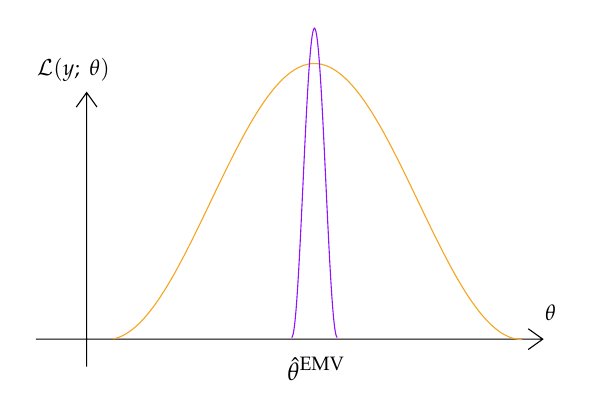
\begin{tikzpicture}[x=0.75pt,y=0.75pt,yscale=-1,xscale=1]
%uncomment if require: \path (0,300); %set diagram left start at 0, and has height of 300

%Shape: Axis 2D [id:dp33309643030277414] 
\draw  (48,169.8) -- (292.17,169.8)(72.42,51) -- (72.42,183) (285.17,164.8) -- (292.17,169.8) -- (285.17,174.8) (67.42,58) -- (72.42,51) -- (77.42,58)  ;
%Shape: Wave [id:dp761793702798415] 
\draw  [color={rgb, 255:red, 245; green, 166; blue, 35 }  ,draw opacity=1 ] (282.17,170) .. controls (264.07,170) and (248.47,137.57) .. (232.17,103.5) .. controls (215.86,69.43) and (200.26,37) .. (182.17,37) .. controls (164.07,37) and (148.47,69.43) .. (132.17,103.5) .. controls (116.77,135.67) and (102,166.38) .. (85.17,169.7) ;
%Shape: Wave [id:dp8411747217824341] 
\draw  [color={rgb, 255:red, 144; green, 19; blue, 254 }  ,draw opacity=1 ] (193.17,169) .. controls (191.18,169) and (189.46,132.67) .. (187.67,94.5) .. controls (185.87,56.33) and (184.16,20) .. (182.17,20) .. controls (180.18,20) and (178.46,56.33) .. (176.67,94.5) .. controls (174.87,132.67) and (173.16,169) .. (171.17,169) ;

% Text Node
\draw (183,184) node  [font=\small] [align=left] {$\displaystyle \hat{\theta}^{\text{EMV}}$};
% Text Node
\draw (296,157) node  [font=\footnotesize] [align=left] {$\displaystyle \theta $};
% Text Node
\draw (66,40) node  [font=\footnotesize] [align=left] {$\displaystyle \mathcal{L}( y;\ \theta )$};


\end{tikzpicture}

On peut donc voir que la forme de la fonction de vraisemblance est plus comprimée, alias que la concavité est plus forte, que l'autre fonction qui se maximise au même point. C'est-à-dire. la fonction de vraisemblance correspond à la fonction avec \textit{la plus forte concavité} dont le maximum est à $\hat{\theta}^{\text{EMV}}_{n}$.	\\

On peut observer que plus la concavité augmente, plus la variabilité de la fonction de vraisemblance se rapetisse. En effet, une faible concavité implique que la fonction de vraisemblance a un grand étendue de valeurs possibles et moins de points près de $\hat\theta^{\text{EMV}}$. En bref, \lfbox[imphl]{la deuxième dérivée assure que}, parmi les fonctions se maximisant à $\hat{\theta}^{\text{EMV}}_{n}$, \lfbox[imphl]{la fonction de vraisemblance est celle dont la variabilité des prévisions est minimisée}.	\\

L'information de Fisher permet de quantifier cette fonction de la deuxième dérivée. Puis, la borne de Cramér-Rao se défini comme son réciproque $1 / \bm{I}(\theta)$. L'intuition est que plus la concavité est faible, plus l'étendue est grand. Prendre le réciproque de l'information de Fisher permet donc de quantifier l'agrandissement de l'étendu.\\

Lorsque l'information de Fisher tend vers l'infini (alias la force de la concavité croît infiniment), on dit que la distribution de l'estimateur est "asymptotiquement normale" tel que $\hat\theta^{\text{EMV}} \overset{a.s.}{\rightarrow} \mathcal{N}\Big(\mu = \theta, \sigma^{2} = \frac{1}{\bm{I}(\theta)}\Big)$ où a.s. veut dire \hyperlink{asympto}{asymptotiquement}.

\columnbreak
\subsubsection{Efficacité}
\begin{distributions}[Notation]
\begin{description}[font = \normalfont]
	\item[$\text{eff}(\hat{\theta}_{n})$]	Efficacité d'un estimateur $\hat{\theta}_{n}$;
	\item[$\text{eff}(\hat\theta_{n}, \tilde\theta_{n})$]	Efficacité de l'estimateur $\hat{\theta}_{n}$ relatif à l'estimateur $\tilde{\theta}_{n}$.
\end{description}
\end{distributions}

Avec le concept de l'information de Fisher, on défini \textbf{l'efficacité d'un estimateur} comme le ratio de la borne Cramér-Rao sur la variance de l'estimateur:
\begin{algo}{Efficacité d'un estimateur}
\begin{align*}
	\text{eff}(\hat{\theta}_{n})
	&=	\frac{\text{Var}(\hat{\theta}_{n})^{\text{Rao}}}{\text{Var}(\hat{\theta})} 
	=	\frac{1}{\bm{I}(\theta)\text{Var}(\hat{\theta})}
\end{align*}
\tcbline
\begin{description}
	\item[Estimateur \og \textit{efficient} \fg{}]	Lorsque la variance de l'estimateur $\text{Var}(\hat{\theta}_{n})$ est égale à la borne de Cramér-Rao.
		\begin{align*}
		\text{eff}(\hat{\theta}_{n}) = 1
		\end{align*}
	\begin{itemize}[leftmargin = *]
	\item	Étant égale à la borne, il \textit{doit} être l'estimateur avec la plus petite de tous les estimateurs sans biais.\\
	 		On dit qu'il est le \og \textbf{\textit{Minimum Variance Unbiased Estimator (MVUE)}} \fg{}. 
	\end{itemize}
\end{description}
\end{algo}

De plus, on peut généraliser cette formulation pour obtenir l'efficacité relative d'un estimateur à un autre:
\begin{algo}{Efficacité relative}
\begin{align*}
	\text{eff}(\hat\theta_{n}, \tilde\theta_{n})
	&=	\frac{\text{Var}(\hat\theta_{n})}{\text{Var}(\tilde\theta_{n})}		\\
\end{align*}
où les estimateurs $\hat\theta_{n}$ et $\tilde\theta_{n}$ sont sans biais.
\tcbline
Lorsque:
\begin{description}[font = \normalfont]
	\item[$\text{eff}(\hat\theta_{n}, \tilde\theta_{n}) < 1$:]	L'estimateur $\hat{\theta}_{n}$ est plus efficace que l'estimateur $\tilde{\theta}_{n}$, \\
	et vice-versa si $\text{eff}(\hat\theta_{n}, \tilde\theta_{n}) > 1$.
\end{description}
\end{algo}

\columnbreak
\subsubsection{Convergence}
Nous pouvons également évaluer si un estimateur converge avec des très grands échantillons; ceci évalue si un estimateur est cohérent. Un estimateur $\hat{\theta}_{n}$ est dit d'être \og \textit{\textbf{consistent}} \fg{} si la probabilité que sa prévision $\hat{\theta}$ du paramètre $\theta$ diffère de la vraie valeur par une erreur, près de 0, $\epsilon$ tend vers 0 alors que la taille de l'échantillon $n$ tend vers l'infini:
\begin{algo}{Convergence (\textbf{consistency}) d'un estimateur}
\begin{align*}
	\underset{n \rightarrow \infty}{\lim} \Pr(\big| \hat{\theta}_{n} - \theta \big| > \epsilon) = 0, \quad \epsilon > 0
\end{align*}
\end{algo}

Ce critère pour qu'un estimateur $\hat{\theta}_{n}$ soit \og \textit{consistent} \fg{} peut être satisfait lorsque: 
\begin{enumerate}
	\item	l'estimateur est \hypertarget{asympto}{\textbf{asymptotiquement sans biais}};
		\begin{align*}
		\limz{n}{\infty} \text{B}(\hat{\theta}_{n}) = 0
		\end{align*}
	\item	la \textbf{variance de l'estimateur tend vers 0}.
		\begin{align*}
		\limz{n}{\infty} \text{Var}(\hat{\theta}_{n}) = 0
		\end{align*}
\end{enumerate}

D'ailleurs, nous avons déjà raisonné ceci avec \hyperlink{cramer-rao}{la borne inférieure Cramér-Rao}.

Cependant, l'inverse n'est pas vrai---qu'un estimateur soit \og \textit{consistent} \fg{} n'implique pas que sa variance ni que son biais tendent vers 0.\\

Malgré la nature plaisante de la convergence d'un estimateur, beaucoup d'estimateurs ont cette propriété. 
Nous voulons alors une mesure qui n'indique pas seulement qu'un estimateur arrive près de la bonne valeur souvent \textit{(alias, une très petite variance)}, mais qu'il est mieux que d'autres estimateurs.
De plus, dût à la sélection arbitraire de l'erreur $\epsilon$ pour la \textit{consistency} d'un estimateur, il est possible de la choisir malicieusement afin de faire parler les données comme on le souhaite. 

\subsubsection*{Détails sur la convergence}
On reprend les résultats de la section précédente en expliquant plus en détails la mathématique sous-jacente.\\

\begin{definitionNOHFILLsub}[Convergence en probabilité]
\begin{distributions}[Notation]
\begin{description}
	\item[$\{Y_{n}\}$]	Séquence de variables aléatoires;
	\item[$Y$]	Variable aléatoire comprise dans $\{Y_{n}\}$.
\end{description}
\end{distributions}

On dit que $Y_{n}$ converge en probabilité à $Y$ si \lfbox[conditions]{$\forall \varepsilon > 0$}, 
\begin{align*}
	\limz{n}{\infty} \Pr\left[|Y_{n}	-	Y|	\geq	\varepsilon\right]	
	&=	0
\end{align*}
%%%	--------------------
%%%	NOTES:
%%%	+	\geq ou > ???
%%%	--------------------
ou de façon équivalente,
\begin{align*}
	\limz{n}{\infty} \Pr\left[|Y_{n}	-	Y|<	\varepsilon\right]	
	&=	1
\end{align*}

On dénote la convergence en probabilité par: \lfbox[formula]{$Y_{n}	\overset{P}{\rightarrow}	Y$.}
\end{definitionNOHFILLsub}

\paragraph{Note:}	La convergence en probabilité est d'ailleurs le théorème sous-jacent à la loi faible des grands nombres vue en prob.

\begin{rappel}{Loi faible des grands nombres}
\begin{distributions}[Notation]
\begin{description}
	\item[$\{Y_{n}\}$]	Séquence de variables aléatoires iid avec moyenne $\mu$ et variance $\sigma^{2}$ où \lfbox[conditions]{$\sigma^{2}	<	\infty$};
	\item[$\overline{X}_{n}$]	Moyenne empirique.
\end{description}
\end{distributions}

On pose que \lfbox[formula]{$\overline{X}_{n}	\overset{P}{\rightarrow}	\mu$.}
\end{rappel}

\begin{definitionNOHFILLsub}[Théorèmes résultant de la convergence en probabilité]
Soit \lfbox[conditions]{$X_{n}	\overset{P}{\rightarrow}	X$} et \lfbox[conditions]{$Y_{n}	\overset{P}{\rightarrow}	Y$}. Alors \lfbox[formula]{$X_{n} + Y_{n}	\overset{P}{\rightarrow}	X + Y$}.\\
Soit \lfbox[conditions]{$X_{n}	\overset{P}{\rightarrow}	X$} et une \lfbox[conditions]{constante $a$}. Alors \lfbox[formula]{$aX_{n}	\overset{P}{\rightarrow}	aX$}.\\
Soit \lfbox[conditions]{$X_{n}	\overset{P}{\rightarrow}	a$} et la \lfbox[conditions]{fonction $g(\cdot)$ continue à $a$}. Alors \lfbox[formula]{$g(X_{n})	\overset{P}{\rightarrow}	g(a)$}.\\
Soit \lfbox[conditions]{$X_{n}	\overset{P}{\rightarrow}	X$} et la \lfbox[conditions]{fonction continue $g(\cdot)$}. Alors \lfbox[formula]{$g(X_{n})	\overset{P}{\rightarrow}	g(X)$}.\\
Soit \lfbox[conditions]{$X_{n}	\overset{P}{\rightarrow}	X$} et \lfbox[conditions]{$Y_{n}	\overset{P}{\rightarrow}	Y$}. Alors \lfbox[formula]{$X_{n}Y_{n}	\overset{P}{\rightarrow}	XY$}.
\end{definitionNOHFILLsub}

\begin{definitionNOHFILL}[\og \textit{Consistency} \fg{}]
\begin{distributions}[Notation]
\begin{description}
	\item[$Y$]	Variable aléatoire avec une distribution paramétrique de paramètre $\theta$;
	\item[$\{Y_{1}, Y_{2}, \dots, Y_{n}\}$]	Échantillon de la distribution de $Y$;
	\item[$\hat{\theta}_{n}$]	Estimateur de $\theta$.
\end{description}
\end{distributions}

On dit que $\hat{\theta}_{n}$ est un estimateur \og \textit{consistent} \fg{} si \lfbox[formula]{$\hat{\theta}_{n}	\overset{P}{\rightarrow}	\theta$}.
\end{definitionNOHFILL}


\subsubsection{Erreur quadratique moyenne}
\begin{distributions}[Notation]
\begin{description}
	\item[$\text{MSE}_{\hat{\theta}_{n}}(\theta)$]	Erreur quadratique moyenne d'un estimateur $\hat{\theta}_{n}$
\end{description}
\end{distributions}

On défini alors l'\textbf{Erreur Quadratique Moyenne} (EQM), ou \textbf{Mean Squared Error (MSE)}, permettant de comparer les différents estimateurs ayant tous une bonne \textit{consistency} en assurant une cohérence d'interprétation. Cette mesure permet de quantifier l'écart entre un estimateur $\hat{\theta}_{n}$ et le vrai paramètre $\theta$.

\begin{algo}{Erreur Quadratique Moyenne (Mean Squared Error)}
\begin{align*}
	\text{MSE}_{\hat\theta}(\theta)
	&=	\text{E}[(\hat{\theta}_{n} - \theta)^{2}]
	\Leftrightarrow	\text{Var}(\hat{\theta}_{n}) + \left[\text{B}(\hat{\theta}_{n})\right]^{2}
\end{align*}
\end{algo}

En combinant tous ces critères, le meilleur estimateur est alors l'estimateur \textbf{sans biais} ayant la \textbf{plus petite variance} possible parmi tous les estimateurs \textit{sans biais}. C'est-à-dire, le \textbf{Uniformly Minimum Variance Unbiased Estimator \textit{(UMVUE)}}.

\columnbreak

\subsection{Estimation par intervalles}
\label{sec:int-estimation}
\begin{distributions}[Notation]
\begin{description}
	\item[$\hat{\theta}_{L}$ et $\hat{\theta}_{U}$]	Fonctions de l'échantillon aléatoire $\{X_{1}, \dots, X_{n}\}$ où \icbox[red][palechestnut]{$\hat{\theta}_{L} < \hat{\theta}_{U}$};
	\item[$(\hat{\theta}_{L}, \hat{\theta}_{U})$]	Intervalle de confiance de $100(1 - \alpha)\%$ de $\theta$ si \icbox[red][palechestnut]{$\Pr(\hat{\theta}_{L} \leq \theta \leq \hat{\theta}_{U}) = 1 - \alpha$};
		\begin{itemize}
		\item	Avec les réalisations, on a un intervalle de nombres réels $(\hat{\theta}_{l}, \hat{\theta}_{u})$.
		\end{itemize}
	\item[$(1 - \alpha)$]	Niveau de confiance de l'intervalle où \lfbox[conditions]{$\alpha \in (0, 1)$}.
\end{description}
\end{distributions}

Le type principal d'estimateur par intervalle est l'\textbf{intervalle de confiance}:
\begin{algo}{Intervalle de confiance}
Nous sommes confiants à un niveau de 100$(1 - \alpha)$\% que le paramètre inconnu $\theta$ est entre $(\hat{\theta}_{L}, \hat{\theta}_{U})$. 

De façon équivalente, nous sommes confiant à un seuil de $\alpha$\% que $\theta$ est entre $(\hat{\theta}_{L}, \hat{\theta}_{U})$.\\

Donc, \icbox{$\theta \in (\hat{\theta}_{L}, \hat{\theta}_{U})$} et nous pouvons dire que \icbox{$\Pr( \hat{\theta}_{L} \le \theta \le  \hat{\theta}_{U}) \ge (1 - \alpha)$} \icbox[red][palechestnut]{pour tout $\theta$}.
\end{algo}

Ce qu'il faut bien saisir avec les intervalles de confiance, c'est que \lfbox[imphl]{soit $\theta$ est contenu dans l'intervalle $(\hat{\theta}_{l}, \hat{\theta}_{u})$ ou il ne l'est pas}.

On peut conceptualiser les intervalles comme une distribution binomiale avec probabilité de succès de $(1 - \alpha)$. Si l'on effectue $M$ essais indépendants, on s'attend à ce que $(1 - \alpha)M$ intervalles de confiance contiennent $\theta$. Donc on se sent confiant à $(1 - \alpha)\%$ que la vraie valeur de $\theta$ est contenue dans l'intervalle observé $(\hat{\theta}_{l}, \hat{\theta}_{u})$.

\paragraph{Efficacité des intervalles de confiance}
Typiquement, la largeur de l'intervalle $(\hat{\theta}_{L}, \hat{\theta}_{U})$ augmente si on augmente le niveau de confiance $(1 - \alpha)$. Par exemple, pour être certain à 100\% que l'intervalle va contenir la valeur, on a qu'à faire un intervalle $(-\infty, \infty)$.\\

Donc, un intervalle plus petit nous donne plus d'information si le niveau est adéquat. On dit que pour un même niveau $(1 - \alpha)$, l'intervalle avec la plus petite largeur est \textit{plus efficace} que l'autre.

\subsubsection{Statistiques}
\begin{rappel_enhanced}[Rappel : Loi du khi-carré]
Soit un échantillon aléatoire $(X_{1}, X_{2}, \dots, X_{n})$ de variables aléatoires normales de moyenne $\mu$ et variance $\sigma^{2}$.\\
Soit \lfbox[formula]{$Q	=	\sumz{n}{i	=	1}\left(X_{i}	-	\mu\right)^{2}$}.\\

Alors, \lfbox[formula]{$Q/\sigma^{2} \sim \chi^{2}_{(n)}$}.
\end{rappel_enhanced}

\begin{rappel_enhanced}[Rappel : Loi de Student]
Soit les variables aléatoires indépendantes :
\begin{itemize}
	\item	$Z \sim \mathcal{N}(0, 1)$.
	\item	$W \sim \chi^{2}_{(n)}$.
\end{itemize}

Alors, \lfbox[formula]{$T	=	\frac{Z}{\sqrt{W/n}}	\sim	t_{(n)}$}.\\

\tcbline

La loi de Student tend vers la normale lorsque $n$ est très grand.
\end{rappel_enhanced}

\begin{rappel_enhanced}[Rappel : Loi de Fisher-Snedecor ($F$)]
Soit les variables aléatoires indépendantes :
\begin{itemize}
	\item	$W_{1} \sim \chi^{2}_{(\nu_{1})}$.
	\item	$W_{2} \sim \chi^{2}_{(\nu_{2})}$.
\end{itemize}

Alors, \lfbox[formula]{$F	=	\frac{W_{1}/\nu_{1}}{W_{2}/\nu_{2}}	\sim	\mathcal{F}_{(\nu_{1}, \nu_{2})}$}.\\

\tcbline

On peut relier la loi de Student et la loi F : \lfbox[formula]{$T^{2}	=	\frac{Z^{2}}{W/n}	\sim	\mathcal{F}_{(1, n)}$} puisque \lfbox[formula]{$Z^{2} \sim \chi^{2}_{(1)}$} où \lfbox[conditions]{$Z \sim \mathcal{N}(0, 1)$}.
\end{rappel_enhanced}

\begin{definitionNOHFILL}[Statistique de test $T_{n}$]
$T_{n}$ est une statistique de test basée sur un échantillon aléatoire de $n$ observations.

\begin{itemize}
\item	C'est donc une \textbf{fonction} d'un échantillon aléatoire ;
\item	Sa distribution est la \textbf{distribution d'échantillonnage} qui dépend de :
	\begin{enumerate}
	\item	La statistique.
	\item	La taille de l'échantillon.
	\item	La distribution sous-jacente des données.
	\end{enumerate}
\end{itemize}
\end{definitionNOHFILL}

\begin{definitionNOHFILLprop}[Moyenne échantillonale $\bar{X}$]
\lfbox[formula]{$\bar{X}	=	\frac{\sum^{n}_{i = 1} X_{i}}{n}$}.

\begin{itemize}
	\item	Estime sans biais la moyenne $\mu$ ;
	\item	Si on pose que l'échantillon aléatoire est normalement distribué, $\bar{X}	\sim \mathcal{N}(\mu, \frac{\sigma}{\sqrt{n}})$ ;
	\item	On centre et réduit pour trouver que \lfbox[formula]{$T_{n}	=	\frac{\bar{X} - \mu}{\sigma/\sqrt{n}} \sim \mathcal{N}(0, 1)$} ;
	\item	Si $\sigma^{2}$ est inconnue, on l'estime avec $s^{2}_{n}$ pour obtenir une distribution student---\lfbox[formula]{$T_{n}	=	\frac{\bar{X} - \mu}{S_{n}/\sqrt{n}}	=	\frac{Z}{\sqrt{W/(n - 1)}} \sim t_{(n - 1)}$} où $W \sim \chi^{2}_{(n - 1)}$.
\end{itemize}
\end{definitionNOHFILLprop}

\begin{definitionNOHFILLprop}[Variance échantillonale $S^{2}_{n}$]
\lfbox[formula]{$S^{2}_{n}	=	\frac{\sum (X_{i} - \bar{X})^{2}}{n - 1}$}.

\begin{itemize}
	\item	Estime \underline{sans biais} la vraie variance $\sigma^{2}$ ;
	\item	$S^{2}_{n}$ n'est pas normalement distribuée, cependant la statistique \lfbox[formula]{$T_{n}	=	\frac{(n - 1)S^{2}_{n}}{\sigma^{2}} \sim \chi^{2}_{(n - 1)}$}.
\end{itemize}
\end{definitionNOHFILLprop}

\begin{definitionNOHFILLprop}[Variance empirique $\hat{\sigma}^{2}$]
\lfbox[formula]{$\hat{\sigma}^{2}	=	\frac{\sum (X_{i} - \bar{X})^{2}}{n}$}.

\begin{itemize}
	\item	Estime \underline{avec biais} la vraie variance $\sigma^{2}$.
\end{itemize}
\end{definitionNOHFILLprop}

\begin{definitionNOHFILLprop}[Statistique $F$]
\lfbox[formula]{$F	=	\frac{S^{2}_{n}/\sigma^{2}_{1}}{S^{2}_{m}/\sigma^{2}_{2}}$}.

\begin{itemize}
	\item	Si on pose que les deux échantillons aléatoires indépendants $(X_{1}, \dots, X_{n})$ et $(Y_{1}, \dots, Y_{m})$ sont normalement distribués, \lfbox[formula]{$F \sim \mathcal{F}_{(n - 1, m - 1)}$}.
\end{itemize}
\end{definitionNOHFILLprop}

\paragraph{Note sur majuscule vs minuscule}	On écrit les statistiques avec des majuscule lorsqu'elle sont aléatoires et avec des minuscules lorsque ce sont des réalisations. Par exemple, dans une probabilité on utilise une majuscule puisque la statistique est aléatoire. 
Pour un seuil $\alpha$ \textbf{\underline{fixé}} d'un intervalle de confiance, le quantile n'est pas aléatoire et jusqu'à ce que l'on calcule l'intervalle avec l'échantillon observé, les statistiques sont également aléatoires. 

\columnbreak
\subsubsection{Intervalles de confiance}
%
%De façon générale, les intervalles de confiance ont une estimation ponctuelle à laquelle on ajoute une marge d'erreur.

\begin{definitionNOHFILLsub}[Intervalle de confiance sur la variance]
%%%	https://www.youtube.com/watch?v=qwqB5a7_W44
Pour l'échantillon aléatoire $\{X_{1}, X_{2}, \dots, X_{n}\}$ issu d'une distribution normale avec $\sigma^{2}$ inconnue, \lfbox[formula]{$\Pr\left(\chi^{2}_{1 - \alpha/2} \leq \frac{(n - 1)S^{2}_{n}}{\sigma^{2}} \leq \chi^{2}_{\alpha/2}\right) =	(1 - \alpha)$}. \\

Graphiquement: 
\begin{center}
\tikzset{every picture/.style={line width=0.75pt}} %set default line width to 0.75pt        

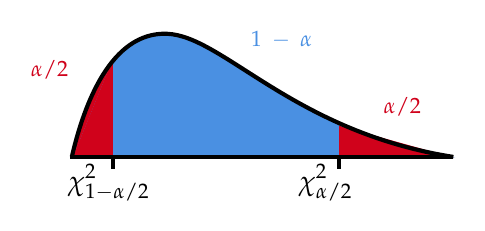
\begin{tikzpicture}[x=0.75pt,y=0.75pt,yscale=-1,xscale=1]
%uncomment if require: \path (0,300); %set diagram left start at 0, and has height of 300

%Curve Lines [id:da6253759692396421] 
\draw [draw opacity=0][fill={rgb, 255:red, 74; green, 144; blue, 226 }  ,fill opacity=1 ][line width=1.5]    (100.83,100.33) .. controls (106.67,75) and (119.67,40) .. (146.67,41) .. controls (173.67,42) and (207.67,88.33) .. (284.67,100.33) ;
%Straight Lines [id:da9705044831224325] 
\draw [draw opacity=0][fill={rgb, 255:red, 208; green, 2; blue, 27 }  ,fill opacity=1 ]   (119.83,52.67) -- (119.83,99.33) -- (100.83,99.33) ;
%Curve Lines [id:da9090824147972125] 
\draw [draw opacity=0][fill={rgb, 255:red, 208; green, 2; blue, 27 }  ,fill opacity=1 ][line width=2.25]    (100.83,99.33) .. controls (106.67,72) and (114.83,58.67) .. (119.83,52.67) ;

%Straight Lines [id:da8243679921312423] 
\draw [draw opacity=0][fill={rgb, 255:red, 208; green, 2; blue, 27 }  ,fill opacity=1 ]   (228.83,85) -- (228.83,100.33) -- (283.83,100.33) ;
%Curve Lines [id:da07655100443368612] 
\draw [line width=1.5]    (100,100) .. controls (105.83,74.67) and (118.83,39.67) .. (145.83,40.67) .. controls (172.83,41.67) and (206.83,88) .. (283.83,100) ;
%Straight Lines [id:da5824849118650262] 
\draw [line width=1.5]    (119.83,100.33) -- (119.83,105.67) ;
%Straight Lines [id:da7912407501617629] 
\draw [line width=1.5]    (228.83,100.33) -- (228.83,105.67) ;
%Straight Lines [id:da26335370673771696] 
\draw [line width=1.5]    (99,100) -- (283.83,100) ;

% Text Node
\draw (79,52) node [anchor=north west][inner sep=0.75pt]  [font=\footnotesize,color={rgb, 255:red, 208; green, 2; blue, 27 }  ,opacity=1 ] [align=left] {$\displaystyle \alpha /2$};
% Text Node
\draw (249,70) node [anchor=north west][inner sep=0.75pt]  [font=\footnotesize,color={rgb, 255:red, 208; green, 2; blue, 27 }  ,opacity=1 ] [align=left] {$\displaystyle \alpha /2$};
% Text Node
\draw (185,38) node [anchor=north west][inner sep=0.75pt]  [font=\footnotesize,color={rgb, 255:red, 74; green, 144; blue, 226 }  ,opacity=1 ] [align=left] {$\displaystyle 1\ -\ \alpha $};
% Text Node
\draw (96.83,102.33) node [anchor=north west][inner sep=0.75pt]   [align=left] {$\displaystyle \chi ^{2}_{1-\alpha /2}$};
% Text Node
\draw (208,102.33) node [anchor=north west][inner sep=0.75pt]   [align=left] {$\displaystyle \chi ^{2}_{\alpha /2}$};


\end{tikzpicture}
\end{center}

Nous sommes donc confiants à un niveau de 100$(1 - \alpha)$\% que :
\begin{align*}
	\sigma^{2} \in \left[
		\frac{(n - 1)S^{2}_{n}}{\chi^{2}_{\alpha / 2}}, 
		\frac{(n - 1)S^{2}_{n}}{\chi^{2}_{1 - \alpha / 2}}
	\right]
\end{align*}
\end{definitionNOHFILLsub}

\begin{definitionNOHFILLsub}[Intervalle de confiance sur la moyenne ($\sigma^{2}$ connue)]
%%%	https://www.youtube.com/watch?v=KG921rfbTDw&list=PLvxOuBpazmsMdPBRxBTvwLv5Lhuk0tuXh&index=4&t=0s
%%%	https://www.youtube.com/watch?v=-iYDu8flFXQ&list=PLvxOuBpazmsMdPBRxBTvwLv5Lhuk0tuXh&index=3&t=268s
Pour l'échantillon aléatoire $\{X_{1}, X_{2}, \dots, X_{n}\}$ issu d'une distribution normale avec $\mu$ inconnu et $\sigma^{2}$ connue, \lfbox[formula]{$\Pr\left(-z_{\alpha/2} \leq \frac{\bar{X} - \mu}{\sigma/\sqrt{n}} \leq z_{\alpha/2}\right) =	(1 - \alpha)$}.\\

Graphiquement:
\begin{center}


\tikzset{every picture/.style={line width=0.75pt}} %set default line width to 0.75pt        

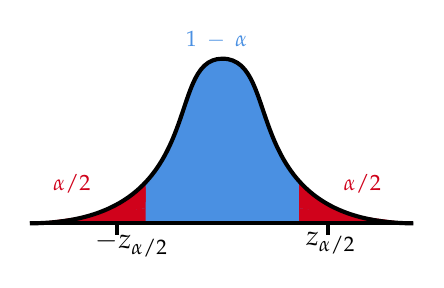
\begin{tikzpicture}[x=0.75pt,y=0.75pt,yscale=-1,xscale=1]
%uncomment if require: \path (0,176); %set diagram left start at 0, and has height of 176

%Curve Lines [id:da8947130044196236] 
\draw [draw opacity=0][fill={rgb, 255:red, 74; green, 144; blue, 226 }  ,fill opacity=1 ][line width=1.5]    (387,99) .. controls (474.83,98.67) and (450.83,19.67) .. (479.83,19.67) .. controls (509.83,19.67) and (485.83,98.67) .. (571.83,99) ;
%Straight Lines [id:da8407133508917781] 
\draw [line width=1.5]    (428.83,99.33) -- (428.83,104.67) ;
%Straight Lines [id:da7153733396293662] 
\draw [line width=1.5]    (530.83,99.33) -- (530.83,104.67) ;
%Straight Lines [id:da1468161753341053] 
\draw [draw opacity=0][fill={rgb, 255:red, 208; green, 2; blue, 27 }  ,fill opacity=1 ]   (516.83,91.67) -- (516.83,99) -- (571.83,99) ;
%Straight Lines [id:da44372694181119354] 
\draw [draw opacity=0][fill={rgb, 255:red, 208; green, 2; blue, 27 }  ,fill opacity=1 ]   (516.83,81.67) -- (516.83,91.67) -- (540.5,95.67) ;
%Straight Lines [id:da871067588661014] 
\draw [draw opacity=0][fill={rgb, 255:red, 208; green, 2; blue, 27 }  ,fill opacity=1 ]   (516.83,78.67) -- (516.83,88.67) -- (528.67,93.67) ;

%Straight Lines [id:da7000317622260974] 
\draw [draw opacity=0][fill={rgb, 255:red, 208; green, 2; blue, 27 }  ,fill opacity=1 ]   (442.83,91.67) -- (442.83,99) -- (387.83,99) ;
%Straight Lines [id:da8176903889743383] 
\draw [draw opacity=0][fill={rgb, 255:red, 208; green, 2; blue, 27 }  ,fill opacity=1 ]   (442.83,81.67) -- (442.83,91.67) -- (419.17,95.67) ;
%Straight Lines [id:da7955659226488763] 
\draw [draw opacity=0][fill={rgb, 255:red, 208; green, 2; blue, 27 }  ,fill opacity=1 ]   (442.83,78.67) -- (442.83,88.67) -- (431,93.67) ;

%Curve Lines [id:da21189166086741196] 
\draw [line width=1.5]    (387,99) .. controls (474.83,98.67) and (450.83,19.67) .. (479.83,19.67) .. controls (509.83,19.67) and (485.83,98.67) .. (571.83,99) ;
%Straight Lines [id:da9615401029487891] 
\draw [line width=1.5]    (387,99) -- (571.83,99) ;


% Text Node
\draw (397,74) node [anchor=north west][inner sep=0.75pt]  [font=\footnotesize,color={rgb, 255:red, 208; green, 2; blue, 27 }  ,opacity=1 ] [align=left] {$\displaystyle \alpha /2$};
% Text Node
\draw (537,74) node [anchor=north west][inner sep=0.75pt]  [font=\footnotesize,color={rgb, 255:red, 208; green, 2; blue, 27 }  ,opacity=1 ] [align=left] {$\displaystyle \alpha /2$};
% Text Node
\draw (461,5) node [anchor=north west][inner sep=0.75pt]  [font=\footnotesize,color={rgb, 255:red, 74; green, 144; blue, 226 }  ,opacity=1 ] [align=left] {$\displaystyle 1\ -\ \alpha $};
% Text Node
\draw (518.83,102) node [anchor=north west][inner sep=0.75pt]   [align=left] {$\displaystyle z_{\alpha /2}$};
% Text Node
\draw (417.33,102) node [anchor=north west][inner sep=0.75pt]   [align=left] {$\displaystyle -z_{\alpha /2}$};


\end{tikzpicture}
\end{center}


Nous sommes donc confiants à un niveau de 100$(1 - \alpha)$\% que :
\begin{equation*}
	\mu \in \left[ \bar{X} - z_{\alpha/2} \frac{\sigma}{\sqrt{n}}, \bar{X} + z_{\alpha/2} \frac{\sigma}{\sqrt{n}}\right].
\end{equation*}
\end{definitionNOHFILLsub}

\begin{definitionNOHFILLsub}[Intervalle de confiance sur la moyenne ($\sigma^{2}$ inconnue)]
Pour l'échantillon aléatoire $\{X_{1}, X_{2}, \dots, X_{n}\}$ issu d'une distribution normale avec $\sigma^{2}$ inconnue, \lfbox[formula]{$\Pr\left(-t_{\alpha/2, n - 1} \leq \frac{\bar{X} - \mu}{S_{n}/\sqrt{n}} \leq t_{\alpha/2, n - 1}\right) =	(1 - \alpha)$}.\\

Graphiquement:
\begin{center}
\tikzset{every picture/.style={line width=0.75pt}} %set default line width to 0.75pt        

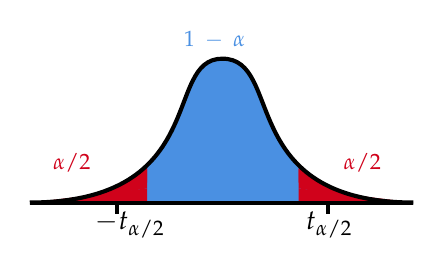
\begin{tikzpicture}[x=0.75pt,y=0.75pt,yscale=-1,xscale=1]
%uncomment if require: \path (0,176); %set diagram left start at 0, and has height of 176

%Curve Lines [id:da982458578172261] 
\draw [draw opacity=0][fill={rgb, 255:red, 74; green, 144; blue, 226 }  ,fill opacity=1 ][line width=1.5]    (386,98) .. controls (473.83,97.67) and (449.83,28.67) .. (478.83,28.67) .. controls (508.83,28.67) and (484.83,97.67) .. (570.83,98) ;
%Straight Lines [id:da3849016484089105] 
\draw [line width=1.5]    (427.83,98.33) -- (427.83,103.67) ;
%Straight Lines [id:da40648686188300065] 
\draw [line width=1.5]    (529.83,98.33) -- (529.83,103.67) ;
%Straight Lines [id:da0901743854683843] 
\draw [draw opacity=0][fill={rgb, 255:red, 208; green, 2; blue, 27 }  ,fill opacity=1 ]   (515.5,91.15) -- (515.5,98) -- (570.83,98) ;
%Straight Lines [id:da7611083055876529] 
\draw [draw opacity=0][fill={rgb, 255:red, 208; green, 2; blue, 27 }  ,fill opacity=1 ]   (515.5,81.8) -- (515.5,91.15) -- (539.31,94.89) ;
%Straight Lines [id:da39003595249115297] 
\draw [draw opacity=0][fill={rgb, 255:red, 208; green, 2; blue, 27 }  ,fill opacity=1 ]   (515.5,79) -- (515.5,88.34) -- (527.41,93.02) ;

%Straight Lines [id:da438403114586448] 
\draw [draw opacity=0][fill={rgb, 255:red, 208; green, 2; blue, 27 }  ,fill opacity=1 ]   (442.5,91.15) -- (442.5,98) -- (386.83,98) ;
%Straight Lines [id:da963730012359405] 
\draw [draw opacity=0][fill={rgb, 255:red, 208; green, 2; blue, 27 }  ,fill opacity=1 ]   (442.5,81.8) -- (442.5,91.15) -- (418.55,94.89) ;
%Straight Lines [id:da7346871172050706] 
\draw [draw opacity=0][fill={rgb, 255:red, 208; green, 2; blue, 27 }  ,fill opacity=1 ]   (442.5,79) -- (442.5,88.34) -- (430.52,93.02) ;

%Curve Lines [id:da971478425929696] 
\draw [line width=1.5]    (386,98) .. controls (473.83,97.67) and (449.83,28.67) .. (478.83,28.67) .. controls (508.83,28.67) and (484.83,97.67) .. (570.83,98) ;
%Straight Lines [id:da9295821978585093] 
\draw [line width=1.5]    (386,98) -- (570.83,98) ;

% Text Node
\draw (396,73) node [anchor=north west][inner sep=0.75pt]  [font=\footnotesize,color={rgb, 255:red, 208; green, 2; blue, 27 }  ,opacity=1 ] [align=left] {$\displaystyle \alpha /2$};
% Text Node
\draw (536,73) node [anchor=north west][inner sep=0.75pt]  [font=\footnotesize,color={rgb, 255:red, 208; green, 2; blue, 27 }  ,opacity=1 ] [align=left] {$\displaystyle \alpha /2$};
% Text Node
\draw (459,14) node [anchor=north west][inner sep=0.75pt]  [font=\footnotesize,color={rgb, 255:red, 74; green, 144; blue, 226 }  ,opacity=1 ] [align=left] {$\displaystyle 1\ -\ \alpha $};
% Text Node
\draw (517.83,101) node [anchor=north west][inner sep=0.75pt]   [align=left] {$\displaystyle t_{\alpha /2}$};
% Text Node
\draw (416.33,101) node [anchor=north west][inner sep=0.75pt]   [align=left] {$\displaystyle -t_{\alpha /2}$};


\end{tikzpicture}
\end{center}

Nous sommes donc confiants à un niveau de 100$(1 - \alpha)$\% que :
\begin{equation*}
	\mu \in \left[ \bar{X} - t_{\alpha/2, n - 1} \frac{S_{n}}{\sqrt{n}}, \bar{X} + t_{\alpha/2, n - 1} \frac{S_{n}}{\sqrt{n}}\right].
\end{equation*}
\end{definitionNOHFILLsub}


%%%	-------------------------
%%%	NOTES:
%%%	+	À retravailler cette section pour ajouter un peu plus de contexte sur les grands échantillons
%%%	-------------------------


\begin{definitionNOHFILLsub}[Intervalle de confiance \textit{approximatif} sur la moyenne]
%%%	https://www.youtube.com/watch?v=bFefxSE5bmo&list=PLvxOuBpazmsMdPBRxBTvwLv5Lhuk0tuXh&index=8&t=0s
Pour l'échantillon aléatoire $\{X_{1}, X_{2}, \dots, X_{n}\}$ issu d'une distribution avec moyenne $\mu$ et une variance inconnue.\\

Pour $n$ très grand, nous sommes \textit{approximativement} confiants à un niveau de 100$(1 - \alpha)$\% que :
\begin{equation*}
	\mu \in \left[ \bar{X} - z_{\alpha/2} \frac{s}{\sqrt{n}}, \bar{X} + z_{\alpha/2} \frac{s}{\sqrt{n}}\right].
\end{equation*}
\end{definitionNOHFILLsub}

\begin{definitionNOHFILLsub}[Intervalle de confiance \textit{approximatif} sur la proportion]
Pour l'échantillon aléatoire $\{X_{1}, X_{2}, \dots, X_{n}\}$ issu d'une distribution Bernoulli de paramètre $p$.\\

Pour $n$ très grand, nous sommes \textit{approximativement} confiants à un niveau de 100$(1 - \alpha)$\% que :
\begin{equation*}
	p \in \left[ \hat{p} - z_{\alpha/2} \sqrt{\frac{\hat{p}(1 - \hat{p})}{n}}, \hat{p} + z_{\alpha/2} \sqrt{\frac{\hat{p}(1 - \hat{p})}{n}}\right].
\end{equation*}
\end{definitionNOHFILLsub}

On défini le \og \textit{pooled estimator} \fg{} comme la moyenne pondérée des deux variances échantillonnales \lfbox[formula]{$S_{p}^{2}	=	\frac{(n - 1)S_{n}^{2} + (m - 1)S_{m}^{2}}{n + m - 2}$}.\\


\begin{definitionNOHFILLsub}[Intervalle de confiance pour une différence de moyennes]
Pour les échantillons aléatoires $\{X_{1}, X_{2}, \dots, X_{n}\}$ et $\{Y_{1}, Y_{2}, \dots, Y_{m}\}$ issus de distributions normales de moyennes $\mu_{1}$ et $\mu_{2}$ et variance $\sigma^{2}_{1} = \sigma^{2}_{2} = \sigma^{2}$ inconnues.

Nous sommes confiants à un niveau de 100$(1 - \alpha)$\% que :
\begin{equation*}
	(\mu_{1}	-	\mu_{2}) \in \left[ 
	\bar{x}_{n}	-	\bar{y}_{m}
	\pm	t_{\alpha/2, n + m - 2} S_{p}\sqrt{\frac{1}{n} + \frac{1}{m}} \right].
\end{equation*}
\begin{align*}
\end{align*}
\end{definitionNOHFILLsub}

\begin{definitionNOHFILLsub}[Intervalle de confiance \textit{approximatif} pour une différence de moyennes]
Pour les échantillons aléatoires $\{X_{1}, X_{2}, \dots, X_{n}\}$ et $\{Y_{1}, Y_{2}, \dots, Y_{m}\}$ issus de distributions normales de moyennes $\mu_{1}$ et $\mu_{2}$ et variances $\sigma^{2}_{1}$ et $\sigma^{2}_{2}$ inconnues.\\

Pour $n$ très grand, nous sommes \textit{approximativement} confiants à un niveau de 100$(1 - \alpha)$\% que :
\begin{equation*}
	(\mu_{1}	-	\mu_{2}) \in \left[ 
	\bar{X}_{n}	-	\bar{Y}_{m}
	\pm	z_{\alpha/2} \sqrt{\frac{S_{n}^{2}}{n} + \frac{S_{m}^{2}}{m}} \right].
\end{equation*}
\begin{align*}
\end{align*}
\end{definitionNOHFILLsub}

\begin{definitionNOHFILLsub}[Intervalle de confiance \textit{approximatif} pour une différence de proportions]
Pour les échantillons aléatoires $\{X_{1}, X_{2}, \dots, X_{n}\}$ et $\{Y_{1}, Y_{2}, \dots, Y_{m}\}$ issus de distributions Bernoulli de paramètres $p_{1}$ et $p_{2}$.\\

Pour $n$ très grand, nous sommes \textit{approximativement} confiants à un niveau de 100$(1 - \alpha)$\% que :
\begin{equation*}
	(p_{1}	-	p_{2}) \in \left[ 
	\hat{p}_{1}	-	\hat{p}_{2}
	\pm	z_{\alpha/2} \sqrt{\frac{\hat{p}_{1}(1 - \hat{p}_{1})}{n} + \frac{\hat{p}_{2}(1 - \hat{p}_{2})}{m}} \right].
\end{equation*}
\begin{align*}
\end{align*}
\end{definitionNOHFILLsub}


%%%
%%%	Méthode du pivot
%%%

\columnbreak
\section{Tests d'hypothèses}
\label{sec:hyp-test}
\subsection{Introduction}
\begin{rappel_enhanced}[Contexte]
Les statistiques classiques posent que tout phénomène observable est régi par un \textit{"\textbf{processus}" sous-jacent}.\\
On ne peut jamais savoir exactement ce qu'est ce "processus"; le mieux que l'on peut faire est d'émettre des \textit{\textbf{hypothèses}} vraisemblables sur ce qu'il pourrait être. \\
Par la suite, on analyse les observations en présumant qu'elles sont régies par le processus hypothétique et détermine la \textit{\textbf{vraisemblance des observations}}. On accepte le processus hypothétique si la vraisemblance est suffisamment élevée.
\end{rappel_enhanced}

\begin{distributions}[Notation]
\begin{description}
	\item[$\Theta_{0}$ et $\Theta_{1}$]	Sous-ensembles disjoints de $\Theta$ tel que \lfbox[formula]{$\Theta_{0} \cup \Theta_{1}	=	\Theta$;}
	\item[$\textrm{H}_{0}$]	Hypothèse nulle ;
		\begin{itemize}
		\item	Représente généralement le statu quo jusqu'à preuve contraire.
		\end{itemize}
	\item[$\textrm{H}_{1}$]	Hypothèse alternative.
		\begin{itemize}
		\item	Représente généralement un changement du statu quo.
		\end{itemize}
\end{description}
\end{distributions}

\begin{definitionNOHFILL}[Test d'hypothèse]
On spécifie une \textcolor{burntorange}{hypothèse} nulle et par conséquent une hypothèse alternative :
\begin{align*}
	\textrm{H}_{0}
	&:	\theta \in \Theta_{0}	&
	&\text{vs}	&
	\textrm{H}_{1}
	&:	\theta \in \Theta_{1}	\\
\end{align*}

Puis, on spécifie une \textcolor{orange-red}{expérience} et un \textcolor{orange}{test} pour décider si l'on accepte ou rejette l'hypothèse nulle.
\end{definitionNOHFILL}

\begin{distributions}[Terminologie]
\begin{description}
\item[\hypertarget{hyp-simple}{Hypothèse simple}]	Spécifie \textbf{entièrement} une distribution de probabilité.
	\begin{itemize}
	\item	Par exemple, $\mathcal{H}_{0}	:	q = 0.50$---on connaît la valeur exacte du paramètre $q$ pour une distribution Bernoulli.
	\end{itemize}
\item[Hypothèse composite]	Spécifie \textbf{partiellement} une distribution de probabilité.
	\begin{itemize}
	\item	Par exemple, $\mathcal{H}_{1}	:	q \neq 0.50$.---on ne connaît pas la valeur exacte du paramètre $q$, il pourrait être n'importe quel chiffre sauf $0.50$.
	\end{itemize}
\end{description}
\end{distributions}

\begin{formula}{Exemple du laissez-passer universitaire (LPU)}
\textcolor{orange-red}{Par exemple}, on veut savoir si le monde utilisent l'autobus (oui ou non) avant et après l'implantation du LPU.\\ 
On \textcolor{burntorange}{pose} que la proportion des gens qui utilisent l'autobus est $q	=	0.44$.\\
Il y a deux types de \textcolor{orange}{tests} qu'on peut faire,
\begin{itemize}
	\item	Tester si l'utilisation est différente est un test "\textbf{bilatéral}", car on test si elle a augmentée \textit{ou} diminuée;
		\begin{align*}
		\textrm{H}_{0}
		&:	q	=	0.44	&
		\textrm{H}_{1}
		&:	q	\neq	0.44
		\end{align*}
	\item	Tester si l'utilisation a augmentée est un test "\textbf{unilatéral}", car on test uniquement si elle a augmentée.
		\begin{align*}
		\textrm{H}_{0}
		&:	q	=	0.44	&
		\textrm{H}_{1}
		&:	q	>	0.44
		\end{align*}
\end{itemize}

Un test unilatéral requiert que l'on sache déjà que la proportion de gens "\textit{doit}" être supérieure. Un test bilatéral est plus conservatif et test les deux possibilités, il devrait donc être celui qu'on applique par défaut. \\

L'hypothèse :
\begin{description}
	\item[nulle]		dans les deux cas est que, en moyenne, l'utilisation de l'autobus n'a pas \textit{changée}. 
	\item[alternative]	dans le cas d'un test :
		\begin{description}
		\item[unilatéral]	est que, en moyenne, l'utilisation a \textit{augmentée}.
		\item[bilatéral]	est que, en moyenne, l'utilisation a \textit{changée}.
		\end{description}
\end{description}
\end{formula}

\begin{definitionNOHFILLsub}[Région critique]
\begin{distributions}[Notation]
\begin{description}
	\item[$\mathcal{S}$]	"Ensemble" de tous les résultats possible pour l'échantillon aléatoire;
	\item[$\mathcal{C}$]	\textbf{Région critique} du test qui est un sous-ensemble de $\mathcal{S}$.
\end{description}
\end{distributions}

On rejette $\textrm{H}_{0}$ si $\{X_{1}, \dots, X_{n}\} \in \mathcal{C}$.\\
On conserve $\textrm{H}_{0}$ si $\{X_{1}, \dots, X_{n}\} \in \mathcal{C}^{c}$.

\begin{itemize}
	\item	On peut aussi dire \og \textbf{région de rejet} \fg{}.
\end{itemize}
\end{definitionNOHFILLsub}

\begin{formula}{Exemple du laissez-passer universitaire (LPU)}
On reprend l'exemple du LPU.\\
L'ensemble des résultats possibles est $\mathcal{S} = [0, 1]$.
\begin{itemize}
	\item	Un test "\textbf{bilatéral}" a comme région critique $\mathcal{C} = [0, 0.44) \cup (0.44, 1]$;
	\item	Un test "\textbf{unilatéral}" testant l'augmentation a comme région critique $\mathcal{C} = (0.44, 1]$.
\end{itemize}
\end{formula}

On peut donc faire 2 types d'erreurs:
%%	voir les images que j'ai gardé pour quand je retouche à la matrice de confusion dans les GLMs pour développer et parler des métriques ! 
\begin{center}
\tikzset{every picture/.style={line width=0.75pt}} %set default line width to 0.75pt        

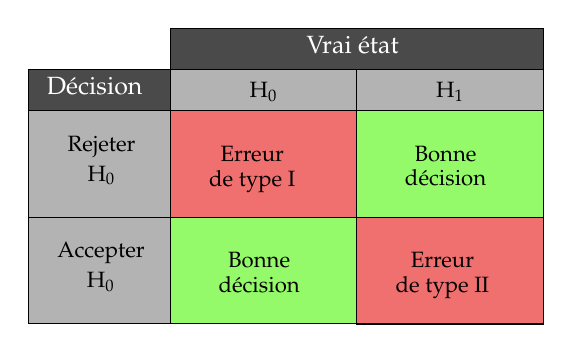
\begin{tikzpicture}[x=0.75pt,y=0.75pt,yscale=-1,xscale=1]
%uncomment if require: \path (0,165); %set diagram left start at 0, and has height of 165

%Shape: Rectangle [id:dp5658804967739193] 
\draw  [fill={rgb, 255:red, 240; green, 111; blue, 111 }  ,fill opacity=1 ] (74,50.17) -- (163.83,50.17) -- (163.83,101.5) -- (74,101.5) -- cycle ;
%Shape: Rectangle [id:dp933461228347003] 
\draw  [fill={rgb, 255:red, 240; green, 111; blue, 111 }  ,fill opacity=1 ] (163.83,101.5) -- (253.67,101.5) -- (253.67,152.83) -- (163.83,152.83) -- cycle ;
%Shape: Rectangle [id:dp24194313951746427] 
\draw  [fill={rgb, 255:red, 148; green, 250; blue, 106 }  ,fill opacity=1 ] (163.83,50) -- (253.67,50) -- (253.67,101.33) -- (163.83,101.33) -- cycle ;
%Shape: Rectangle [id:dp27324261874552724] 
\draw  [fill={rgb, 255:red, 148; green, 250; blue, 106 }  ,fill opacity=1 ] (74,101.33) -- (163.83,101.33) -- (163.83,152.67) -- (74,152.67) -- cycle ;
%Shape: Rectangle [id:dp9425087952138109] 
\draw  [fill={rgb, 255:red, 179; green, 179; blue, 179 }  ,fill opacity=1 ] (74,30.17) -- (163.83,30.17) -- (163.83,50) -- (74,50) -- cycle ;
%Shape: Rectangle [id:dp40513736937576916] 
\draw  [fill={rgb, 255:red, 74; green, 74; blue, 74 }  ,fill opacity=1 ] (74,10.33) -- (253.67,10.33) -- (253.67,30.17) -- (74,30.17) -- cycle ;
%Shape: Rectangle [id:dp4099498200973881] 
\draw  [fill={rgb, 255:red, 179; green, 179; blue, 179 }  ,fill opacity=1 ] (163.83,30.17) -- (253.67,30.17) -- (253.67,50) -- (163.83,50) -- cycle ;
%Shape: Rectangle [id:dp35293578825776084] 
\draw  [fill={rgb, 255:red, 179; green, 179; blue, 179 }  ,fill opacity=1 ] (5.5,101.33) -- (74,101.33) -- (74,152.67) -- (5.5,152.67) -- cycle ;
%Shape: Rectangle [id:dp2841127241620307] 
\draw  [fill={rgb, 255:red, 179; green, 179; blue, 179 }  ,fill opacity=1 ] (5.5,50.17) -- (74,50.17) -- (74,101.5) -- (5.5,101.5) -- cycle ;
%Shape: Rectangle [id:dp5918283025493905] 
\draw  [fill={rgb, 255:red, 74; green, 74; blue, 74 }  ,fill opacity=1 ] (5.5,30.33) -- (74,30.33) -- (74,50.17) -- (5.5,50.17) -- cycle ;

% Text Node
\draw (138.33,13) node [anchor=north west][inner sep=0.75pt]  [font=\small,color={rgb, 255:red, 255; green, 255; blue, 255 }  ,opacity=1 ] [align=left] {Vrai état};
% Text Node
\draw (110.92,35) node [anchor=north west][inner sep=0.75pt]  [font=\footnotesize,color={rgb, 255:red, 0; green, 0; blue, 0 }  ,opacity=1 ] [align=left] {$ \text{H}_{0}$};
% Text Node
\draw (200.75,35) node [anchor=north west][inner sep=0.75pt]  [font=\footnotesize,color={rgb, 255:red, 0; green, 0; blue, 0 }  ,opacity=1 ] [align=left] {$ \text{H}_{1}$};
% Text Node
\draw (18.25,112) node [anchor=north west][inner sep=0.75pt]  [font=\footnotesize,color={rgb, 255:red, 0; green, 0; blue, 0 }  ,opacity=1 ] [align=left] {\shortstack{Accepter\\ $\text{H}_{0}$}};
% Text Node
\draw (23.25,60.83) node [anchor=north west][inner sep=0.75pt]  [font=\footnotesize,color={rgb, 255:red, 0; green, 0; blue, 0 }  ,opacity=1 ] [align=left] {\shortstack{Rejeter\\ $\text{H}_{0}$}};
% Text Node
\draw (13.25,32.75) node [anchor=north west][inner sep=0.75pt]  [font=\small,color={rgb, 255:red, 255; green, 255; blue, 255 }  ,opacity=1 ] [align=left] {Décision};
% Text Node
\draw (91.42,65.83) node [anchor=north west][inner sep=0.75pt]  [font=\footnotesize,color={rgb, 255:red, 0; green, 0; blue, 0 }  ,opacity=1 ] [align=left] 
{\shortstack{Erreur\\ de type I}};
% Text Node
\draw (181.25,117) node [anchor=north west][inner sep=0.75pt]  [font=\footnotesize,color={rgb, 255:red, 0; green, 0; blue, 0 }  ,opacity=1 ] [align=left] {\shortstack{Erreur\\ de type II}};
% Text Node
\draw (95.92,117) node [anchor=north west][inner sep=0.75pt]  [font=\footnotesize,color={rgb, 255:red, 0; green, 0; blue, 0 }  ,opacity=1 ] [align=left] {\shortstack{Bonne\\ décision}};
% Text Node
\draw (185.75,65.67) node [anchor=north west][inner sep=0.75pt]  [font=\footnotesize,color={rgb, 255:red, 0; green, 0; blue, 0 }  ,opacity=1 ] [align=left] {\shortstack{Bonne\\ décision}};



\end{tikzpicture}
\end{center}

\columnbreak
\subsection{Certitude du test}
Lorsque nous voulons quantifier le degré auquel nous sommes confiants du test, nous utilisons la valeur $p$. \\
La valeur $p$ a trois composantes:
\begin{enumerate}
	\item	La probabilité que l'événement se produise aléatoirement.
	\item	La probabilité qu'un événement tout aussi rare se produise.
	\item	La probabilité qu'un événement encore plus rare se produise.
\end{enumerate}

\begin{formula}{Exemple de pile ou face}
On souhaite tester si, en obtenant deux piles sur deux lancers, nous avons une pièce de monnaie truquée :
\begin{description}
	\item[Hypothèse nulle]	Ma pièce de monnaie n'est pas truquée même si j'ai obtenu deux piles.
\end{description}
\

Étapes du calcul de la valeur $p$:
\begin{enumerate}
	\item	On calcule la probabilité d'obtenir 2 piles: $0.5 \times 0.5 = 0.25$.
	\item	Puis, on calcule la probabilité d'obtenir 2 faces (un événement autant rare): $0.5 \times 0.5 = 0.25$.
	\item	Finalement, il n'y a pas d'autres séquences plus rares.
\end{enumerate}
Donc, la valeur $p$ du test est de $0.50$.

\begin{itemize}
	\item	Ceci est plutôt élevé;
	\item	Souvent, on pose que la valeur $p$ du test doit être d'au plus $0.05$;
	\item	Ce qui veut dire que des événements tout aussi (ou plus) rares doivent arriver moins que 5\% du temps pour que l'on considère la pièce de monnaie comme étant truquée;
	\item	Donc, dans notre cas, on ne peut pas rejeter l'hypothèse nulle que notre pièce de monnaie n'est pas spéciale.
\end{itemize}
\end{formula}

Dans le cas continu, on somme les probabilités d'être plus rare ou d'être moins rare. C'est la même idée que les intervalles de confiance avec la valeur $p$, ou \textit{seuil de signifiance $\alpha$}, représenté en rouge. 
\begin{itemize}
	\item	Si la valeur $p$ est petite, ceci indique que d'autres distributions pourraient potentiellement mieux s'ajuster aux données puisque l'événement est très rare;
	\item	Si la valeur $p$ est grande, ceci indique que l'événement est très courant et que la distribution semble être bien ajustée.
\end{itemize}

\

Il y a plusieurs termes semblables qui peuvent devenir mélangeants.
\begin{distributions}[Terminologie]
\begin{description}
	\item[$p$]	La \textbf{valeur $p$} du test.
		\begin{itemize}
		\item	On peut la définir comme la probabilité d'un événement autant (ou plus) rare sous l'hypothèse nulle ;
		\item	On peut la définir comme la \textbf{taille} de la région critique $\mathcal{C}$ ; c'est-à-dire, l'\textit{aire} de la région de rejet de l'hypothèse nulle $\text{H}_{0}$ alors qu'elle est vraie ;
		\item	On peut la définir comme le \textbf{seuil de signifiance} ; c'est-à-dire, la probabilité de rejeter $\text{H}_{0}$ alors qu'elle est vraie ;
		\item	Elle correspond donc également à la \textbf{probabilité d'une erreur de type I}.
		\end{itemize}
	\item[$\alpha$]	Dénote habituellement le \textbf{seuil de signifiance} ou la \textbf{taille} du test.
		\begin{itemize}
		\item	Même idée qu'avec les intervalles de confiance;
		\item	On peut parfois aussi utiliser $\alpha$ pour dénoter la valeur de $p$ qui détermine si on rejette ou pas un test ;
		\item	En anglais, \og \textit{threshold for significance} \fg{}.
		\end{itemize}
\end{description}
\end{distributions}

Formellement, on défini \lfbox[formula]{$\alpha	=	{\color{indigo(web)}\max}_{{\color{amethyst}\theta} \in {\color{pastelred}\Theta_{0}}} \Pr\left\{{\color{bondiblue!80!black}(X_{1}, \dots, X_{n})} {\color{armygreen}\in} {\color{bulgarianrose}\mathcal{C}} ; {\color{amethyst}\theta} \right\}$}. \\
C'est-à-dire :
\begin{itemize}
	\item	on \textcolor{indigo(web)}{maximise} la probabilité que \textcolor{bondiblue!80!black}{l'échantillon aléatoire} soit \textcolor{armygreen}{contenu} dans \textcolor{bulgarianrose!90!black}{la région critique} (alias rejeter $\textrm{H}_{0}$), 
	\item	où la distribution est tracée \textcolor{amethyst}{en fonction du paramètre $\theta$} de \textcolor{pastelred}{l'hypothèse nulle}.
\end{itemize}


\columnbreak
\subsection{Puissance d'un test}
\begin{definitionNOHFILL}[La puissance d'un test]
La probabilité de \textit{correctement} rejeter l'hypothèse nulle.
%%	https://www.youtube.com/watch?v=Rsc5znwR5FA&feature=youtu.be

\tcbline

Une analyse de la puissance détermine le nombre d'observations qu'il faut afin d'avoir une probabilité élevée de correctement rejeter l'hypothèse nulle.
\end{definitionNOHFILL}


Plusieurs facteurs influencent la puissance d'un test. Lorsqu'on teste si deux échantillons d'observations proviennent de la même distribution,
\begin{definitionNOHFILLsub}[La forme de la distribution]
Si les deux distributions sont:
\begin{itemize}
	\item	Très \textbf{distinctes}, la puissance sera très \textbf{élevée}:
		\begin{center}
		\tikzset{every picture/.style={line width=0.75pt}} %set default line width to 0.75pt        

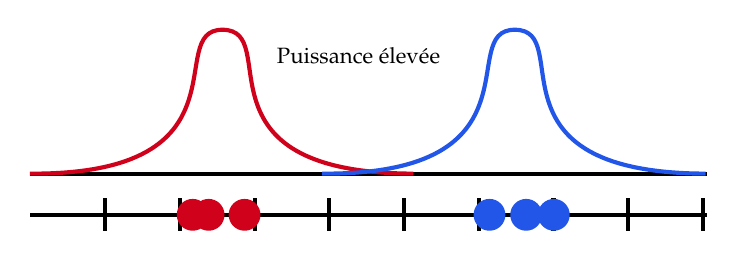
\begin{tikzpicture}[x=0.75pt,y=0.75pt,yscale=-1,xscale=1]
%uncomment if require: \path (0,176); %set diagram left start at 0, and has height of 176

%Straight Lines [id:da864976542619565] 
\draw [line width=1.5]    (245.5,117.83) -- (571.5,117.83) (281.5,109.83) -- (281.5,125.83)(317.5,109.83) -- (317.5,125.83)(353.5,109.83) -- (353.5,125.83)(389.5,109.83) -- (389.5,125.83)(425.5,109.83) -- (425.5,125.83)(461.5,109.83) -- (461.5,125.83)(497.5,109.83) -- (497.5,125.83)(533.5,109.83) -- (533.5,125.83)(569.5,109.83) -- (569.5,125.83) ;
%Straight Lines [id:da9295821978585093] 
\draw [line width=1.5]    (245.17,98) -- (571.5,98) ;
%Curve Lines [id:da28384300225010417] 
\draw [color={rgb, 255:red, 208; green, 2; blue, 27 }  ,draw opacity=1 ][line width=1.5]    (245.17,98) .. controls (353.67,98.67) and (309,28.67) .. (338,28.67) .. controls (368,28.67) and (320.67,97.67) .. (430,98) ;
%Curve Lines [id:da19190888762749303] 
\draw [color={rgb, 255:red, 33; green, 86; blue, 233 }  ,draw opacity=1 ][line width=1.5]    (386,98) .. controls (494.5,98.67) and (449.83,28.67) .. (478.83,28.67) .. controls (508.83,28.67) and (461.5,97.67) .. (570.83,98) ;
%Shape: Circle [id:dp23295532013997544] 
\draw  [draw opacity=0][fill={rgb, 255:red, 208; green, 2; blue, 27 }  ,fill opacity=1 ] (316,117.83) .. controls (316,113.6) and (319.43,110.17) .. (323.67,110.17) .. controls (327.9,110.17) and (331.33,113.6) .. (331.33,117.83) .. controls (331.33,122.07) and (327.9,125.5) .. (323.67,125.5) .. controls (319.43,125.5) and (316,122.07) .. (316,117.83) -- cycle ;
%Shape: Circle [id:dp6583442494748755] 
\draw  [draw opacity=0][fill={rgb, 255:red, 208; green, 2; blue, 27 }  ,fill opacity=1 ] (323.67,117.83) .. controls (323.67,113.6) and (327.1,110.17) .. (331.33,110.17) .. controls (335.57,110.17) and (339,113.6) .. (339,117.83) .. controls (339,122.07) and (335.57,125.5) .. (331.33,125.5) .. controls (327.1,125.5) and (323.67,122.07) .. (323.67,117.83) -- cycle ;
%Shape: Circle [id:dp7278683126625956] 
\draw  [draw opacity=0][fill={rgb, 255:red, 208; green, 2; blue, 27 }  ,fill opacity=1 ] (341,117.83) .. controls (341,113.6) and (344.43,110.17) .. (348.67,110.17) .. controls (352.9,110.17) and (356.33,113.6) .. (356.33,117.83) .. controls (356.33,122.07) and (352.9,125.5) .. (348.67,125.5) .. controls (344.43,125.5) and (341,122.07) .. (341,117.83) -- cycle ;
%Shape: Circle [id:dp6846096733160589] 
\draw  [draw opacity=0][fill={rgb, 255:red, 33; green, 86; blue, 233 }  ,fill opacity=1 ] (459,117.83) .. controls (459,113.6) and (462.43,110.17) .. (466.67,110.17) .. controls (470.9,110.17) and (474.33,113.6) .. (474.33,117.83) .. controls (474.33,122.07) and (470.9,125.5) .. (466.67,125.5) .. controls (462.43,125.5) and (459,122.07) .. (459,117.83) -- cycle ;
%Shape: Circle [id:dp05843938160550621] 
\draw  [draw opacity=0][fill={rgb, 255:red, 33; green, 86; blue, 233 }  ,fill opacity=1 ] (476.67,117.83) .. controls (476.67,113.6) and (480.1,110.17) .. (484.33,110.17) .. controls (488.57,110.17) and (492,113.6) .. (492,117.83) .. controls (492,122.07) and (488.57,125.5) .. (484.33,125.5) .. controls (480.1,125.5) and (476.67,122.07) .. (476.67,117.83) -- cycle ;
%Shape: Circle [id:dp2540684792866683] 
\draw  [draw opacity=0][fill={rgb, 255:red, 33; green, 86; blue, 233 }  ,fill opacity=1 ] (490,117.83) .. controls (490,113.6) and (493.43,110.17) .. (497.67,110.17) .. controls (501.9,110.17) and (505.33,113.6) .. (505.33,117.83) .. controls (505.33,122.07) and (501.9,125.5) .. (497.67,125.5) .. controls (493.43,125.5) and (490,122.07) .. (490,117.83) -- cycle ;

% Text Node
\draw (363,36) node [anchor=north west][inner sep=0.75pt]  [font=\footnotesize,color={rgb, 255:red, 255; green, 255; blue, 255 }  ,opacity=1 ] [align=left] {\textcolor{black}{Puissance élevée}};


\end{tikzpicture}
		\end{center}
		\begin{itemize}
		\item	 La probabilité de \textbf{correctement} rejeter l'hypothèse nulle (que les deux échantillons proviennent d'une même distribution) est élevée;
		\item	On peut aussi dire qu'il y a une forte probabilité de \textbf{correctement} obtenir une faible valeur $p$.
		\end{itemize}
	\item	Se \textbf{chevauchent}, la puissance sera \textbf{faible}:
		\begin{center}
		\tikzset{every picture/.style={line width=0.75pt}} %set default line width to 0.75pt        

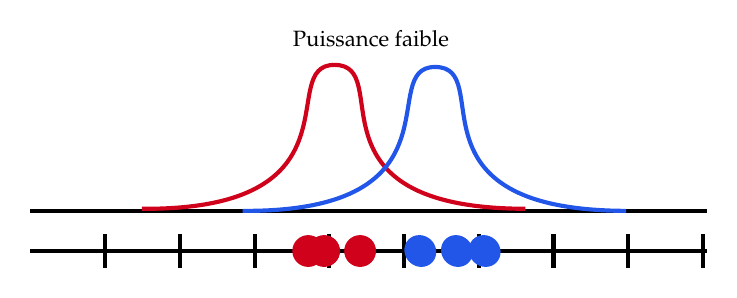
\begin{tikzpicture}[x=0.75pt,y=0.75pt,yscale=-1,xscale=1]
%uncomment if require: \path (0,176); %set diagram left start at 0, and has height of 176

%Straight Lines [id:da674545395459474] 
\draw [line width=1.5]    (244.83,117.33) -- (570.83,117.33) (280.83,109.33) -- (280.83,125.33)(316.83,109.33) -- (316.83,125.33)(352.83,109.33) -- (352.83,125.33)(388.83,109.33) -- (388.83,125.33)(424.83,109.33) -- (424.83,125.33)(460.83,109.33) -- (460.83,125.33)(496.83,109.33) -- (496.83,125.33)(532.83,109.33) -- (532.83,125.33)(568.83,109.33) -- (568.83,125.33) ;
%Shape: Circle [id:dp5899062048279418] 
\draw  [draw opacity=0][fill={rgb, 255:red, 208; green, 2; blue, 27 }  ,fill opacity=1 ] (371,117.33) .. controls (371,113.1) and (374.43,109.67) .. (378.67,109.67) .. controls (382.9,109.67) and (386.33,113.1) .. (386.33,117.33) .. controls (386.33,121.57) and (382.9,125) .. (378.67,125) .. controls (374.43,125) and (371,121.57) .. (371,117.33) -- cycle ;
%Shape: Circle [id:dp033764139219446765] 
\draw  [draw opacity=0][fill={rgb, 255:red, 208; green, 2; blue, 27 }  ,fill opacity=1 ] (378.67,117.33) .. controls (378.67,113.1) and (382.1,109.67) .. (386.33,109.67) .. controls (390.57,109.67) and (394,113.1) .. (394,117.33) .. controls (394,121.57) and (390.57,125) .. (386.33,125) .. controls (382.1,125) and (378.67,121.57) .. (378.67,117.33) -- cycle ;
%Shape: Circle [id:dp9956436610120569] 
\draw  [draw opacity=0][fill={rgb, 255:red, 208; green, 2; blue, 27 }  ,fill opacity=1 ] (396,117.33) .. controls (396,113.1) and (399.43,109.67) .. (403.67,109.67) .. controls (407.9,109.67) and (411.33,113.1) .. (411.33,117.33) .. controls (411.33,121.57) and (407.9,125) .. (403.67,125) .. controls (399.43,125) and (396,121.57) .. (396,117.33) -- cycle ;
%Straight Lines [id:da9463171904376761] 
\draw [line width=1.5]    (244.5,98) -- (570.83,98) ;
%Curve Lines [id:da7529446506143549] 
\draw [color={rgb, 255:red, 208; green, 2; blue, 27 }  ,draw opacity=1 ][line width=1.5]    (298.5,97) .. controls (407,97.67) and (362.33,27.67) .. (391.33,27.67) .. controls (421.33,27.67) and (374,96.67) .. (483.33,97) ;
%Curve Lines [id:da7479872172646262] 
\draw [color={rgb, 255:red, 33; green, 86; blue, 233 }  ,draw opacity=1 ][line width=1.5]    (347,98) .. controls (455.5,98.67) and (410.83,28.67) .. (439.83,28.67) .. controls (469.83,28.67) and (422.5,97.67) .. (531.83,98) ;
%Shape: Circle [id:dp8825558203269679] 
\draw  [draw opacity=0][fill={rgb, 255:red, 33; green, 86; blue, 233 }  ,fill opacity=1 ] (425,117.33) .. controls (424.72,113.1) and (427.93,109.67) .. (432.17,109.67) .. controls (436.4,109.67) and (440.06,113.1) .. (440.33,117.33) .. controls (440.61,121.57) and (437.4,125) .. (433.17,125) .. controls (428.93,125) and (425.28,121.57) .. (425,117.33) -- cycle ;
%Shape: Circle [id:dp2808249488586654] 
\draw  [draw opacity=0][fill={rgb, 255:red, 33; green, 86; blue, 233 }  ,fill opacity=1 ] (442.67,117.33) .. controls (442.39,113.1) and (445.6,109.67) .. (449.83,109.67) .. controls (454.07,109.67) and (457.72,113.1) .. (458,117.33) .. controls (458.28,121.57) and (455.07,125) .. (450.83,125) .. controls (446.6,125) and (442.94,121.57) .. (442.67,117.33) -- cycle ;
%Shape: Circle [id:dp8643138982751464] 
\draw  [draw opacity=0][fill={rgb, 255:red, 33; green, 86; blue, 233 }  ,fill opacity=1 ] (456,117.33) .. controls (455.72,113.1) and (458.93,109.67) .. (463.17,109.67) .. controls (467.4,109.67) and (471.06,113.1) .. (471.33,117.33) .. controls (471.61,121.57) and (468.4,125) .. (464.17,125) .. controls (459.93,125) and (456.28,121.57) .. (456,117.33) -- cycle ;

% Text Node
\draw (370,10) node [anchor=north west][inner sep=0.75pt]  [font=\footnotesize,color={rgb, 255:red, 255; green, 255; blue, 255 }  ,opacity=1 ] [align=left] {\textcolor{black}{Puissance faible}};


\end{tikzpicture}
		\end{center}
		\begin{itemize}
		\item	 La probabilité de \textbf{incorrectement} rejeter l'hypothèse nulle (que les deux échantillons proviennent d'une même distribution) est élevée;
		\item	On peut aussi dire qu'il y a une forte probabilité de \textbf{incorrectement} obtenir une faible valeur $p$;
		\item	Cependant, la puissance peut être augmentée avec plus d'observations.
		\end{itemize}
\end{itemize}
\end{definitionNOHFILLsub}

\begin{definitionNOHFILLsub}[La variabilité des données]
Si la variabilité de la distribution est
\begin{itemize}
	\item	\textbf{Faible}, alors la variabilité de l'échantillon sera probablement faible aussi menant à une puissance très \textbf{élevée}:
		\begin{center}
		\tikzset{every picture/.style={line width=0.75pt}} %set default line width to 0.75pt        

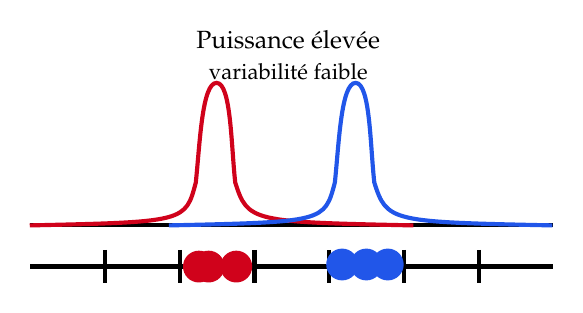
\begin{tikzpicture}[x=0.75pt,y=0.75pt,yscale=-1,xscale=1]
%uncomment if require: \path (0,176); %set diagram left start at 0, and has height of 176

%Straight Lines [id:da864976542619565] 
\draw [line width=1.5]    (245.42,117.83) -- (497.17,117.83) (281.42,109.83) -- (281.42,125.83)(317.42,109.83) -- (317.42,125.83)(353.42,109.83) -- (353.42,125.83)(389.42,109.83) -- (389.42,125.83)(425.42,109.83) -- (425.42,125.83)(461.42,109.83) -- (461.42,125.83) ;
%Straight Lines [id:da9295821978585093] 
\draw [line width=1.5]    (245.17,98) -- (497.17,98) ;
%Shape: Circle [id:dp23295532013997544] 
\draw  [draw opacity=0][fill={rgb, 255:red, 208; green, 2; blue, 27 }  ,fill opacity=1 ] (319,117.83) .. controls (319,113.6) and (322.43,110.17) .. (326.67,110.17) .. controls (330.9,110.17) and (334.33,113.6) .. (334.33,117.83) .. controls (334.33,122.07) and (330.9,125.5) .. (326.67,125.5) .. controls (322.43,125.5) and (319,122.07) .. (319,117.83) -- cycle ;
%Shape: Circle [id:dp6583442494748755] 
\draw  [draw opacity=0][fill={rgb, 255:red, 208; green, 2; blue, 27 }  ,fill opacity=1 ] (323.67,117.83) .. controls (323.67,113.6) and (327.1,110.17) .. (331.33,110.17) .. controls (335.57,110.17) and (339,113.6) .. (339,117.83) .. controls (339,122.07) and (335.57,125.5) .. (331.33,125.5) .. controls (327.1,125.5) and (323.67,122.07) .. (323.67,117.83) -- cycle ;
%Shape: Circle [id:dp7278683126625956] 
\draw  [draw opacity=0][fill={rgb, 255:red, 208; green, 2; blue, 27 }  ,fill opacity=1 ] (337,117.83) .. controls (337,113.6) and (340.43,110.17) .. (344.67,110.17) .. controls (348.9,110.17) and (352.33,113.6) .. (352.33,117.83) .. controls (352.33,122.07) and (348.9,125.5) .. (344.67,125.5) .. controls (340.43,125.5) and (337,122.07) .. (337,117.83) -- cycle ;
%Shape: Circle [id:dp6846096733160589] 
\draw  [draw opacity=0][fill={rgb, 255:red, 33; green, 86; blue, 233 }  ,fill opacity=1 ] (388,116.83) .. controls (388,112.6) and (391.43,109.17) .. (395.67,109.17) .. controls (399.9,109.17) and (403.33,112.6) .. (403.33,116.83) .. controls (403.33,121.07) and (399.9,124.5) .. (395.67,124.5) .. controls (391.43,124.5) and (388,121.07) .. (388,116.83) -- cycle ;
%Shape: Circle [id:dp05843938160550621] 
\draw  [draw opacity=0][fill={rgb, 255:red, 33; green, 86; blue, 233 }  ,fill opacity=1 ] (399.67,116.83) .. controls (399.67,112.6) and (403.1,109.17) .. (407.33,109.17) .. controls (411.57,109.17) and (415,112.6) .. (415,116.83) .. controls (415,121.07) and (411.57,124.5) .. (407.33,124.5) .. controls (403.1,124.5) and (399.67,121.07) .. (399.67,116.83) -- cycle ;
%Shape: Circle [id:dp2540684792866683] 
\draw  [draw opacity=0][fill={rgb, 255:red, 33; green, 86; blue, 233 }  ,fill opacity=1 ] (410,116.83) .. controls (410,112.6) and (413.43,109.17) .. (417.67,109.17) .. controls (421.9,109.17) and (425.33,112.6) .. (425.33,116.83) .. controls (425.33,121.07) and (421.9,124.5) .. (417.67,124.5) .. controls (413.43,124.5) and (410,121.07) .. (410,116.83) -- cycle ;
%Curve Lines [id:da9834393207352259] 
\draw [color={rgb, 255:red, 208; green, 2; blue, 27 }  ,draw opacity=1 ][line width=1.5]    (245.17,98) .. controls (320.17,96.33) and (320.17,96.33) .. (325.17,77.33) .. controls (327.17,58.33) and (328.17,29.33) .. (335.17,29.33) .. controls (342.17,29.33) and (342.17,59.33) .. (344.17,77.33) .. controls (350.17,96.33) and (352.17,96.33) .. (430,98) ;
%Curve Lines [id:da5775597107131041] 
\draw [color={rgb, 255:red, 33; green, 86; blue, 233 }  ,draw opacity=1 ][line width=1.5]    (312.17,98) .. controls (387.17,96.33) and (387.17,96.33) .. (392.17,77.33) .. controls (394.17,58.33) and (395.17,29.33) .. (402.17,29.33) .. controls (409.17,29.33) and (409.17,59.33) .. (411.17,77.33) .. controls (417.17,96.33) and (419.17,96.33) .. (497,98) ;

% Text Node
\draw (324,3) node [anchor=north west][inner sep=0.75pt]  [font=\small,color={rgb, 255:red, 0; green, 0; blue, 0 }  ,opacity=1 ] [align=left] {\begin{minipage}[lt]{66.6825pt}\setlength\topsep{0pt}
\begin{center}
Puissance élevée\\{\footnotesize variabilité faible}
\end{center}

\end{minipage}};


\end{tikzpicture}
		\end{center}
	\item	\textbf{Élevée}, alors la variabilité de l'échantillon sera probablement élevée aussi menant à une puissance \textbf{faible}: 
		\begin{center}
		\tikzset{every picture/.style={line width=0.75pt}} %set default line width to 0.75pt        

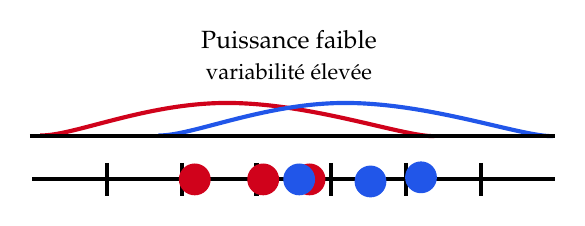
\begin{tikzpicture}[x=0.75pt,y=0.75pt,yscale=-1,xscale=1]
%uncomment if require: \path (0,176); %set diagram left start at 0, and has height of 176

%Straight Lines [id:da224342647816256] 
\draw [line width=1.5]    (291.42,122.83) -- (543.17,122.83) (327.42,114.83) -- (327.42,130.83)(363.42,114.83) -- (363.42,130.83)(399.42,114.83) -- (399.42,130.83)(435.42,114.83) -- (435.42,130.83)(471.42,114.83) -- (471.42,130.83)(507.42,114.83) -- (507.42,130.83) ;
%Shape: Circle [id:dp7289237376471596] 
\draw  [draw opacity=0][fill={rgb, 255:red, 208; green, 2; blue, 27 }  ,fill opacity=1 ] (362,122.83) .. controls (362,118.6) and (365.43,115.17) .. (369.67,115.17) .. controls (373.9,115.17) and (377.33,118.6) .. (377.33,122.83) .. controls (377.33,127.07) and (373.9,130.5) .. (369.67,130.5) .. controls (365.43,130.5) and (362,127.07) .. (362,122.83) -- cycle ;
%Shape: Circle [id:dp6581028616853248] 
\draw  [draw opacity=0][fill={rgb, 255:red, 208; green, 2; blue, 27 }  ,fill opacity=1 ] (417.3,122.83) .. controls (417.3,118.6) and (420.73,115.17) .. (424.96,115.17) .. controls (429.2,115.17) and (432.63,118.6) .. (432.63,122.83) .. controls (432.63,127.07) and (429.2,130.5) .. (424.96,130.5) .. controls (420.73,130.5) and (417.3,127.07) .. (417.3,122.83) -- cycle ;
%Shape: Circle [id:dp32832339728857773] 
\draw  [draw opacity=0][fill={rgb, 255:red, 208; green, 2; blue, 27 }  ,fill opacity=1 ] (394.96,122.83) .. controls (394.96,118.6) and (398.39,115.17) .. (402.63,115.17) .. controls (406.86,115.17) and (410.3,118.6) .. (410.3,122.83) .. controls (410.3,127.07) and (406.86,130.5) .. (402.63,130.5) .. controls (398.39,130.5) and (394.96,127.07) .. (394.96,122.83) -- cycle ;
%Shape: Circle [id:dp8463878803176157] 
\draw  [draw opacity=0][fill={rgb, 255:red, 33; green, 86; blue, 233 }  ,fill opacity=1 ] (412.3,122.83) .. controls (412.3,118.6) and (415.73,115.17) .. (419.96,115.17) .. controls (424.2,115.17) and (427.63,118.6) .. (427.63,122.83) .. controls (427.63,127.07) and (424.2,130.5) .. (419.96,130.5) .. controls (415.73,130.5) and (412.3,127.07) .. (412.3,122.83) -- cycle ;
%Shape: Circle [id:dp41576741952688256] 
\draw  [draw opacity=0][fill={rgb, 255:red, 33; green, 86; blue, 233 }  ,fill opacity=1 ] (446.67,123.83) .. controls (446.67,119.6) and (450.1,116.17) .. (454.33,116.17) .. controls (458.57,116.17) and (462,119.6) .. (462,123.83) .. controls (462,128.07) and (458.57,131.5) .. (454.33,131.5) .. controls (450.1,131.5) and (446.67,128.07) .. (446.67,123.83) -- cycle ;
%Shape: Circle [id:dp7322447345202854] 
\draw  [draw opacity=0][fill={rgb, 255:red, 33; green, 86; blue, 233 }  ,fill opacity=1 ] (471,121.83) .. controls (471,117.6) and (474.43,114.17) .. (478.67,114.17) .. controls (482.9,114.17) and (486.33,117.6) .. (486.33,121.83) .. controls (486.33,126.07) and (482.9,129.5) .. (478.67,129.5) .. controls (474.43,129.5) and (471,126.07) .. (471,121.83) -- cycle ;
%Curve Lines [id:da3201541308920388] 
\draw [color={rgb, 255:red, 208; green, 2; blue, 27 }  ,draw opacity=1 ][line width=1.5]    (295.17,101.67) .. controls (311.17,102) and (346.17,86) .. (385.17,86) .. controls (426.17,86) and (470.33,102.33) .. (485.17,102) ;
%Curve Lines [id:da0520324915772159] 
\draw [color={rgb, 255:red, 33; green, 86; blue, 233 }  ,draw opacity=1 ][line width=1.5]    (352.17,101.67) .. controls (368.17,102) and (403.17,86) .. (442.17,86) .. controls (483.17,86) and (527.33,102.33) .. (542.17,102) ;
%Straight Lines [id:da9874290431386423] 
\draw [line width=1.5]    (290.17,102) -- (543.17,102) ;

% Text Node
\draw (371,50) node [anchor=north west][inner sep=0.75pt]  [font=\small,color={rgb, 255:red, 0; green, 0; blue, 0 }  ,opacity=1 ] [align=left] {\begin{minipage}[lt]{64.149144pt}\setlength\topsep{0pt}
\begin{center}
Puissance faible\\{\footnotesize variabilité élevée}
\end{center}

\end{minipage}};
\end{tikzpicture}
		\end{center}
\end{itemize}
\end{definitionNOHFILLsub}

Il existe plusieurs mesures qui permettent de considérer la variabilité des données ainsi que la forme de la distribution. Entres autre, il y a le \og \textit{\textbf{effect size ($d$)}} \fg{} où \lfbox[formula]{$d	=	\frac{\bar{x} - \bar{y}}{s^{2}_{p}}$}.

\begin{definitionNOHFILLsub}[Le taille de l'échantillon de données]
Un grand échantillon de données peut compenser pour des distributions qui se chevauchent ou une variabilité élevée. Ça permet d'augmenter notre \textit{confiance} qu'il y a bel et bien une différence entre les échantillons. \\

En contraste, nous n'avons pas besoin d'un grand échantillon de données pour des distributions très distinctes ou avec une faible variabilité; nous sommes déjà confiants que les distributions sont différentes.
\end{definitionNOHFILLsub}

\begin{definitionNOHFILLsub}[Le test statistique]
Certains tests ont une puissance plus élevée que les autres. \\
Cela dit, le test $t$ habituel est très puissant.
\end{definitionNOHFILLsub}

\subsubsection{La fonction de puissance}

La fonction de puissance est \lfbox[formula]{$\gamma(\theta)	=	\Pr\left\{(X_{1}, \dots, X_{n}) \in \mathcal{C} ; \theta \right\}$} ; c'est-à-dire, la probabilité de rejeter l'hypothèse nulle $\mathrm{H}_{0}$ si la \textbf{vraie} valeur du paramètre est $\theta \in \Theta$. 
\begin{itemize}
	\item	C'est une fonction de $\theta$ ;
	\item	Idéalement, si l'hypothèse nulle est :
		\begin{description}
		\item[acceptée]	on souhaite que $\gamma(\theta)	=	0$ puisque $\theta \in \Theta_{0}$.
			\begin{itemize}
			\item	On dénote $\gamma(\theta_{0})	=	\Pr\left\{(X_{1}, \dots, X_{n}) \in \mathcal{C} ;  \theta \in \Theta_{0}\right\}	=	0$.
			\end{itemize}
		\item[rejetée]	on souhaite que $\gamma(\theta)	=	1$ puisque $\theta \in \Theta_{1}$.
			\begin{itemize}
			\item	On dénote $\gamma(\theta_{1})	=	\Pr\left\{(X_{1}, \dots, X_{n}) \in \mathcal{C} ; \theta \in \Theta_{1}\right\}	=	1$.
			\end{itemize}
		\end{description}
\end{itemize}

Si, par exemple, on rejette l'hypothèse nulle on pourrait tracer la fonction de puissance pour toutes les valeurs possibles de l'ensemble $\Theta_{1}$.


%%	
%	\lfbox[formula]{$n \geq \left(\frac{z}{k - \mu_{1}}\right)^{2}\sigma^{2}$}.


\columnbreak

\subsection{Tests optimaux}
\begin{distributions}[Notation]
\begin{description}
	\item[$\delta$]	(Procédure de) test ;
	\item[$\alpha(\delta)$]	Probabilité d'une erreur de type I pour un test $\delta$ ;
		\begin{itemize}
		\item	$\alpha(\delta)	=	\Pr\left\{(X_{1}, \dots, X_{n}) \in \mathcal{C} ;  \theta \in \Theta_{0}\right\}	=	\gamma(\theta_{0})$.
		\end{itemize}
	\item[$\beta(\delta)$]	Probabilité d'une erreur de type II pour un test $\delta$ ;
		\begin{itemize}
		\item	$\beta(\delta)	=	\Pr\left\{(X_{1}, \dots, X_{n}) \in \mathcal{C}^{\complement} ;  \theta \in \Theta_{1}\right\}	=	1 - \gamma(\theta_{1})$.
		\end{itemize}
\end{description}

\end{distributions}
Pour mettre en contexte cette notation, revoici le tableau des types d'erreur pour un test $\delta$ :
\begin{center}
\tikzset{every picture/.style={line width=0.75pt}} %set default line width to 0.75pt        

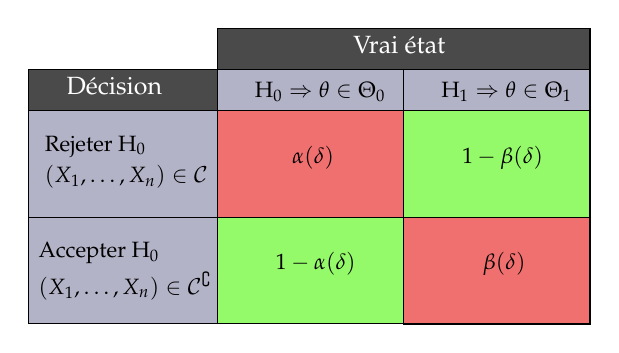
\begin{tikzpicture}[x=0.75pt,y=0.75pt,yscale=-1,xscale=1]
%uncomment if require: \path (0,165); %set diagram left start at 0, and has height of 165

%Shape: Rectangle [id:dp5658804967739193] 
\draw  [fill={rgb, 255:red, 240; green, 111; blue, 111 }  ,fill opacity=1 ] (74,50.17) -- (163.83,50.17) -- (163.83,101.5) -- (74,101.5) -- cycle ;
%Shape: Rectangle [id:dp933461228347003] 
\draw  [fill={rgb, 255:red, 240; green, 111; blue, 111 }  ,fill opacity=1 ] (163.83,101.5) -- (253.67,101.5) -- (253.67,152.83) -- (163.83,152.83) -- cycle ;
%Shape: Rectangle [id:dp24194313951746427] 
\draw  [fill={rgb, 255:red, 148; green, 250; blue, 106 }  ,fill opacity=1 ] (163.83,50) -- (253.67,50) -- (253.67,101.33) -- (163.83,101.33) -- cycle ;
%Shape: Rectangle [id:dp27324261874552724] 
\draw  [fill={rgb, 255:red, 148; green, 250; blue, 106 }  ,fill opacity=1 ] (74,101.33) -- (163.83,101.33) -- (163.83,152.67) -- (74,152.67) -- cycle ;

%Shape: Rectangle [id:dp9425087952138109] 
\draw  [fill={rgb, 255:red, 179; green, 179; blue, 200 }  ,fill opacity=1 ] (74,30.17) -- (163.83,30.17) -- (163.83,50) -- (74,50) -- cycle ;
%Shape: Rectangle [id:dp4099498200973881] 
\draw  [fill={rgb, 255:red, 179; green, 179; blue, 200 }  ,fill opacity=1 ] (163.83,30.17) -- (253.67,30.17) -- (253.67,50) -- (163.83,50) -- cycle ;
%Shape: Rectangle [id:dp35293578825776084] 
\draw  [fill={rgb, 255:red, 179; green, 179; blue, 200 }  ,fill opacity=1 ] (-17,101.33) -- (74,101.33) -- (74,152.67) -- (-17,152.67) -- cycle ;
%Shape: Rectangle [id:dp2841127241620307] 
\draw  [fill={rgb, 255:red, 179; green, 179; blue, 200 }  ,fill opacity=1 ] (-17,50.17) -- (74,50.17) -- (74,101.5) -- (-17,101.5) -- cycle ;

%Shape: Rectangle [id:dp40513736937576916] 
\draw  [fill={rgb, 255:red, 74; green, 74; blue, 74 }  ,fill opacity=1 ] (74,10.33) -- (253.67,10.33) -- (253.67,30.17) -- (74,30.17) -- cycle ;
%Shape: Rectangle [id:dp5918283025493905] 
\draw  [fill={rgb, 255:red, 74; green, 74; blue, 74 }  ,fill opacity=1 ] (-17,30.33) -- (74,30.33) -- (74,50.17) -- (-17,50.17) -- cycle ;

% Text Node
\draw (138.33,13) node [anchor=north west][inner sep=0.75pt]  [font=\small,color={rgb, 255:red, 255; green, 255; blue, 255 }  ,opacity=1 ] [align=left] {Vrai état};
% Text Node
\draw (90.92,35) node [anchor=north west][inner sep=0.75pt]  [font=\footnotesize,color={rgb, 255:red, 0; green, 0; blue, 0 }  ,opacity=1 ] [align=left] {$ \text{H}_{0} \Rightarrow \theta \in \Theta_{0}$};
% Text Node
\draw (180.75,35) node [anchor=north west][inner sep=0.75pt]  [font=\footnotesize,color={rgb, 255:red, 0; green, 0; blue, 0 }  ,opacity=1 ] [align=left] {$ \text{H}_{1} \Rightarrow \theta \in \Theta_{1}$};

% Text Node
\draw (-13.25,112) node [anchor=north west][inner sep=0.75pt]  [font=\footnotesize,color={rgb, 255:red, 0; green, 0; blue, 0 }  ,opacity=1 ] [align=left] {\shortstack[l]{Accepter $\text{H}_{0}$\\ $(X_{1}, \dots, X_{n}) \in \mathcal{C}^{\complement}$ }};
% Text Node
\draw (-10.25,60.83) node [anchor=north west][inner sep=0.75pt]  [font=\footnotesize,color={rgb, 255:red, 0; green, 0; blue, 0 }  ,opacity=1] [align=left] {\shortstack[l]{Rejeter $\text{H}_{0}$\\ $(X_{1}, \dots, X_{n}) \in \mathcal{C}$}};

% Text Node
\draw (0.25,32.75) node [anchor=north west][inner sep=0.75pt]  [font=\small,color={rgb, 255:red, 255; green, 255; blue, 255 }  ,opacity=1 ] [align=left] {Décision};
% Text Node
\draw (108.92,65.83) node [anchor=north west][inner sep=0.75pt]  [font=\footnotesize,color={rgb, 255:red, 0; green, 0; blue, 0 }  ,opacity=1 ] [align=left] 
{$\alpha(\delta)$};
% Text Node
\draw (200.75,117) node [anchor=north west][inner sep=0.75pt]  [font=\footnotesize,color={rgb, 255:red, 0; green, 0; blue, 0 }  ,opacity=1 ] [align=left] {$\beta(\delta)$};
% Text Node
\draw (100.92,117) node [anchor=north west][inner sep=0.75pt]  [font=\footnotesize,color={rgb, 255:red, 0; green, 0; blue, 0 }  ,opacity=1 ] [align=left] {$1 - \alpha(\delta)$};
% Text Node
\draw (190.75,65.67) node [anchor=north west][inner sep=0.75pt]  [font=\footnotesize,color={rgb, 255:red, 0; green, 0; blue, 0 }  ,opacity=1 ] [align=left] {$1 - \beta(\delta)$};
\end{tikzpicture}
\end{center}

\begin{itemize}
	\item	\textit{En théorie}, on minimise la probabilité d'une erreur de type I \textbf{et} de II ; 
	\item	\textit{En réalité}, il y a un compromis et on ne pourra pas avoir des très petites probabilités pour les deux ;
	\item	Le contexte va déterminer ce qu'on souhaite minimiser le plus ;
		\begin{itemize}
		\item	Par exemple, soit l'hypothèse nulle que quelqu'un n'a pas le cancer ;
		\item	Il est plus grave de dire à quelqu'un qu'il n'a pas le cancer alors qu'il l'a (erreur de type II) que de dire qu'il a le cancer alors qu'il ne l'a pas (erreur de type I) ;
		\item	Dans ce contexte, on souhaiterait minimiser l'erreur de type II $\beta(\delta)$ plus que celle de type I $\alpha(\delta)$.
		\end{itemize}
%	\item	Cela dit, on peut tenter de minimiser une \textit{fonction} des deux erreurs.
\end{itemize}

Puisqu'il est impossible de trouver un test $\delta$ pour lequel les probabilités d'erreurs de type I et II sont très petites, on :
\begin{enumerate}
	\item	Fixe l'erreur de type I à un seuil, alias une taille de région critique, $k$.
	\item	Trouve parmi tout les sous-ensembles de taille $k$ celui qui minimise l'erreur de type II.
\end{enumerate}

\begin{definitionNOHFILLprop}[Tests optimaux]
%Puisqu'il est impossible de trouver un test $\delta$ pour lequel les probabilités d'erreurs de type I et II sont très petites, on peut minimiser la fonction \lfbox[formula]{$a\alpha(\delta) + b\beta(\delta)$} des \lfbox[conditions]{constantes $a, b > 0$}.\\

%\tcbline

Soit un test $\delta^{*}$ avec les hypothèses \hyperlink{hyp-simple}{\color{blue!80!white}\underline{simples}} :
\begin{align*}
	\mathrm{H}_{0}	&:	\theta	=	\theta_{0}	\\
	\mathrm{H}_{1}	&:	\theta	=	\theta_{1}
\end{align*}
\begin{itemize}
	\item	Par exemple, on pourrait avoir une distribution Bernoulli et poser $\mathrm{H}_{0}	:	p	=	0.4$ v.s. $\mathrm{H}_{1}	:	p	=	0.6$.
\end{itemize}
\

La procédure pour trouver la région critique $\mathcal{C}$ optimale de taille $\alpha$ du test $\delta^{\ast}$ est la suivante :
\begin{enumerate}
	\item	On trouve une région critique (alias, un sous-ensemble de $\mathcal{S}$) $\mathcal{C}$ tel que la probabilité $\alpha(\delta^{\ast})$ d'une erreur de type I est de $\alpha$.
		\begin{itemize}
		\item	C'est-à-dire, \lfbox[conditions]{$\alpha(\delta^{\ast})	=	Pr\left\{(X_{1}, \dots, X_{n}) \in \mathcal{C} ;  \theta	=	\theta_{0}\right\}	=	\alpha$}.
		\item	Cependant, ce critère n'identifie par un sous-ensemble unique ;
		\item	Il y a une multitude de sous-ensemble $\mathcal{A}$ de $\mathcal{S}$ dont la probabilité que l'échantillon aléatoire y soit contenu (sous l'hypothèse nulle) est aussi $\alpha$ ;
		\item	C'est-à-dire, $Pr\left\{(X_{1}, \dots, X_{n}) \in \mathcal{A}; \theta	=	\theta_{0}	\right\}	=	\alpha$.
		\end{itemize}
	\item	On pose que la probabilité que l'échantillon aléatoire soit dans la région critique $\mathcal{C}$ (sous l'hypothèse alternative) est supérieure à la probabilité que l'échantillon aléatoire soit contenu dans tout autre sous-ensemble $\mathcal{A}$.
		\begin{itemize}
		\item	C'est-à-dire, \lfbox[formula]{$Pr\left\{(X_{1}, \dots, X_{n}) \in \mathcal{C}; \theta	=	\theta_{1}	\right\}	\geq Pr\big\{(X_{1}, \dots, X_{n}) \in \mathcal{A};$} \lfbox[formula]{$\theta	=	\theta_{1}	\big\}$}.
		\end{itemize}
\end{enumerate}

Avec ces deux critères, on trouve \textit{\textbf{la}} région critique $\mathcal{C}$ de taille $\alpha$ \textbf{optimale} pour tester les hypothèses simples.

%%%%	%%%%	%%%%	%%%%	%%%%	%%%%	%%%%	%%%%	%%%%	%%%%	%%%%	
%%%	Test optimal selon les NDC de M.-P.	%%%%	
%\begin{itemize}
%	\item	 $\mathrm{H}_{0}$ est acceptée si \lfbox[conditions]{$af(\bm{x} ; \theta_{0})	>	bf(\bm{x} ; \theta_{1})$} ;
%	\item	 $\mathrm{H}_{0}$ est rejetée si \lfbox[conditions]{$af(\bm{x} ; \theta_{0})	<	bf(\bm{x} ; \theta_{1})$} ;
%	\item	Si \lfbox[conditions]{$af(\bm{x} ; \theta_{0})	=	bf(\bm{x} ; \theta_{1})$} soit $\mathrm{H}_{0}$ ou $\mathrm{H}_{1}$ peut être acceptée.
%\end{itemize}
%
%Pour tout autre test $\delta$, \lfbox[formula]{$a\alpha(\delta^{*}) + b\beta(\delta^{*})	\leq	a\alpha(\delta) + b\beta(\delta)$}.
%%%%	%%%%	%%%%	%%%%	%%%%	%%%%	%%%%	%%%%	%%%%	%%%%	%%%%	
\end{definitionNOHFILLprop}

En bref, on pose fixe à un seuil $\alpha$ la fonction de puissance posant que le vrai paramètre $\theta	=	\theta_{0}$ puis on trouve la région critique qui maximise la puissance posant que le vrai paramètre $\theta	=	\theta_{1}$.

\begin{formula}{Exemple avec une distribution Binomiale}
Soit :
\begin{itemize}
	\item	La variable aléatoire $X \sim Binom(n = 3, p = \theta)$.
		\begin{itemize}
		\item	Alors, $\mathcal{S}	=	\{x : x	=	0, 1, 2, 3\}$.
		\end{itemize}
	\item	Les hypothèses : \\
		\begin{align*}
		\mathrm{H}_{0}	&:	\theta	=	0.50	\\
		\mathrm{H}_{1}	&:	\theta	=	0.75
		\end{align*}
	\item	Le seuil de signifiance $\alpha	=	0.125$.
	\item	Les sous-ensembles $\mathcal{A}_{1}	=	\{x : x = 0\}$ et $\mathcal{A}_{2}	=	\{x : x = 3\}$ de $\mathcal{S}$.
\end{itemize}
Alors, $\Pr( X \in \mathcal{A}_{1}; \theta	=	0.50)	=	\Pr( X \in \mathcal{A}_{2}; \theta	=	0.50)	=	0.125$ et il n'y a pas d'autres sous-ensembles de $\mathcal{S}$ avec la même taille de $0.125$.\\
Il s'ensuit que soit $\mathcal{A}_{1}$ ou $\mathcal{A}_{2}$ est la région critique $\mathcal{C}$ optimale de taille $\alpha$ pour tester $\mathrm{H}_{0}$ contre $\mathrm{H}_{1}$.\\

On trouve que $\Pr( X \in \mathcal{A}_{1}; \theta	=	0.75)	=	0.015625$ alors que $\Pr( X \in \mathcal{A}_{2}; \theta	=	0.75)	=	0.421875$. 
\begin{itemize}
	\item	Dans le premier cas :\\
		\setlength{\mathindent}{-1cm}
		\begin{align*}
		\Pr( \underbrace{X \in \mathcal{A}_{1}; \theta	=	0.75}_{\mathclap{\shortstack{rejeter $\mathrm{H}_{0}$ alors que $\mathrm{H}_{0}$\\ est faux ($\theta = 0.75$)}}})	
		&=	0.015625		&
		&<	&
		\Pr( \underbrace{X \in \mathcal{A}_{1}; \theta	=	0.50}_{\mathclap{\shortstack{rejeter $\mathrm{H}_{0}$ alors que $\mathrm{H}_{0}$\\ est vraie ($\theta = 0.50$)}}})	
		&=	0.125	
		\end{align*}
		\setlength{\mathindent}{1cm}
	\item	Dans le deuxième cas :\\
		\setlength{\mathindent}{-1cm}
		\begin{align*}
		\Pr( \underbrace{X \in \mathcal{A}_{2}; \theta	=	0.75}_{\mathclap{\shortstack{rejeter $\mathrm{H}_{0}$ alors que $\mathrm{H}_{0}$\\ est faux ($\theta = 0.75$)}}})	
		&=	0.421875		&
		&>	&
		\Pr( \underbrace{X \in \mathcal{A}_{2}; \theta	=	0.50}_{\mathclap{\shortstack{rejeter $\mathrm{H}_{0}$ alors que $\mathrm{H}_{0}$\\ est vraie ($\theta = 0.50$)}}})	
		&=	0.125	
		\end{align*}
		\setlength{\mathindent}{1cm}
	\item	Le premier sous-ensemble $\mathcal{A}_{1}$ n'est pas désirable car on serait plus probable de incorrectement rejeter $\mathrm{H}_{0}$ lorsqu'elle est vraie (erreur de type I) que de correctement la rejeter lorsqu'elle est fausse ! 
	\item	Alors, on choisit $\mathcal{C}	=	\mathcal{A}_{2}	=	\{x: x = 3\}$.
\end{itemize}

D'ailleurs, la région est choisie en incluant dans $\mathcal{C}$ les points $x$ pour lesquels $f(x; \theta	=	0.50)$ est petite par rapport à $f(x; \theta	=	0.75)$.
\begin{itemize}
	\item	On peut d'ailleurs observer que le ratio $\frac{f(x; \theta	=	0.50)}{f(x; \theta	=	0.75)}$ évalué à $x	=	5$ est un minimum.
\end{itemize}
\end{formula}

On peut utiliser ce ratio comme outil pour identifier la région critique $\mathcal{C}$ optimale pour un seuil fixe de $\alpha$.


\columnbreak
\subsubsection{Cas d'hypothèses simples}

\begin{definitionNOHFILL}[Théorème de Neymann-Pearson]
%Le lemme de Neyman-Pearson trouve le test $\delta$ qui minimise la probabilité d'une erreur de type II $\beta(\delta)$ parmi tous les test dont la probabilité d'une erreur de type I $\alpha(\delta)$ est inférieure ou égale à 
%$\alpha	=	\alpha(\delta^{*})	=	\Pr\left\{ f(\bm{X} ; \theta_{0}) < k f(\bm{X} ; \theta_{1}) ; \theta \in \Theta_{0} \right\}$.

Soit un test $\delta^{*}$ avec les hypothèses \hyperlink{hyp-simple}{\color{blue!80!white}\underline{simple}} :
\begin{align*}
	\mathrm{H}_{0}	&:	\theta	=	\theta_{0}	\\
	\mathrm{H}_{1}	&:	\theta	=	\theta_{1}
\end{align*}
\

Soit une constante $k > 0$ et le sous-ensemble $\mathcal{C} \in \mathcal{S}$ tel que :
\begin{enumerate}
	\item	\lfbox[formula]{$\frac{\mathcal{L}(\theta_{0} ; \bm{x})}{\mathcal{L}(\theta_{1} ; \bm{x})}	\leq	k$} pour tout \lfbox[conditions]{$x \in \mathcal{C}$}.
	\item	\lfbox[formula]{$\frac{\mathcal{L}(\theta_{0} ; \bm{x})}{\mathcal{L}(\theta_{1} ; \bm{x})}	\geq	k$} pour tout \lfbox[conditions]{$x \in \mathcal{C}^{\complement}$}.
		\begin{itemize}
		\item	En réécrivant les équations comme $\mathcal{L}(\theta_{1} ; \bm{x})	\leq\textcolor{teal}{(\geq)}\	k\mathcal{L}(\theta_{0} ; \bm{x})$ on peut l'interpréter comme qu'il doit être plus vraisemblable que $\theta	=	\theta_{0}\textcolor{teal}{(\theta_{1})}$ que $\theta_{1}\textcolor{teal}{(\theta_{0})}$ lorsque $x \in \mathcal{C}^{\textcolor{teal}{\complement}}$ et que l'on rejette \textcolor{teal}{(accepte)} $\mathrm{H}_{0}$.
		\end{itemize}
	\item	\lfbox[formula]{$\alpha	=	\Pr\left\{ (X_{1}, \dots, X_{n}) \in \mathcal{C}; \theta_{1} \right\}	=	\alpha(\delta^{\ast})$}.
\end{enumerate}

Alors $\mathcal{C}$ est \textbf{\textit{la}} région critique \textbf{optimale} de taille $\alpha$.

%%%%	%%%%	%%%%	%%%%	%%%%	%%%%	%%%%	%%%%	%%%%	%%%%	%%%%	%%%%	
%%%	Neymann-Pearsoon selon les NDC de M.-P.	%%%%	
%\begin{itemize}
%	\item	 $\mathrm{H}_{0}$ est acceptée si \lfbox[conditions]{$f(\bm{x} ; \theta_{0})	>	kf(\bm{x} ; \theta_{1})$} ;
%	\item	 $\mathrm{H}_{0}$ est rejetée si \lfbox[conditions]{$f(\bm{x} ; \theta_{0})	<	kf(\bm{x} ; \theta_{1})$} ;
%	\item	Si \lfbox[conditions]{$f(\bm{x} ; \theta_{0})	=	kf(\bm{x} ; \theta_{1})$} une ou l'autre sera acceptée.
%\end{itemize}
%Si $\delta$ est n'importe quel autre test que $\delta^{*}$ tel que \lfbox[conditions]{$\alpha(\delta) \leq \alpha(\delta^{*})$} alors \lfbox[formula]{$\beta(\delta)	\geq	\beta(\delta^{*})$}.
%\begin{itemize}
%	\item	De façon semblable, si \lfbox[conditions]{$\alpha(\delta) < \alpha(\delta^{*})$} alors \lfbox[formula]{$\beta(\delta)	>	\beta(\delta^{*})$} ;
%\end{itemize}
%%%%	%%%%	%%%%	%%%%	%%%%	%%%%	%%%%	%%%%	%%%%	%%%%	%%%%	%%%%	
\end{definitionNOHFILL}

\begin{definitionNOHFILLsub}[Test non biaisé]
Soit les mêmes hypothèses que dans la définition du théorème de Neymann-Pearson.\\

Un test $\delta$ est non biaisé si sa puissance est toujours d'au moins $\alpha$ ; c'est-à-dire, \lfbox[formula]{$\Pr\left\{(X_{1}, \dots, X_{n}) \in \mathcal{C}; \theta \right\} \geq \alpha$}.\\

Le meilleur test obtenue par le théorème de Neymann-Pearson est non biaisé.
\end{definitionNOHFILLsub}

\begin{formula}{Exemple avec une distribution Normale}
Soit :
\begin{itemize}
	\item	L'échantillon aléatoire $\bm{X}	=	(X_{1}, \dots, X_{n})$ d'une distribution normale $\mathcal{N}(\mu = \theta, \sigma^{2} = 0)$.
		\begin{itemize}
		\item	Alors, $\mathcal{S}	=	\{x : x	\in \mathbb{R}\}$.
		\end{itemize}
	\item	Les hypothèses : 
		\begin{align*}
		\mathrm{H}_{0}	&:	\theta	=	0	\\
		\mathrm{H}_{1}	&:	\theta	=	1
		\end{align*}
\end{itemize}

On a : 
\begin{align*}
	\frac{\mathcal{L}(\theta_{0} ; \bm{x})}{\mathcal{L}(\theta_{1} ; \bm{x})}
	&=	\frac{\textrm{exp}\left\{-\sum_{i = 1}^{n}x^{2}_{i}/2\right\}\frac{1}{(\sqrt{2\pi})^{n}}}{\textrm{exp}\left\{-\sum_{i = 1}^{n}(x_{i} - 1)^{2}/2\right\}\frac{1}{(\sqrt{2\pi})^{n}}}	
	=	\textrm{exp}\left\{-\sum_{i = 1}^{n}x_{i} + \frac{n}{2}\right\}	\\
\end{align*}

Alors, la région critique $\mathcal{C}$ optimale est composée des points $(x_{1}, x_{2}, \dots, x_{n})$ tel que :
\begin{align*}
	\textrm{e}^{-\sum_{i = 1}^{n}x_{i} + \frac{n}{2}}	
	&\leq	k	&
	&\Rightarrow	&
	-\sum_{i = 1}^{n}x_{i} + \frac{n}{2}
	&\leq	\ln(k)	&
	&\Rightarrow	&
	\sum_{i = 1}^{n}x_{i}
	&\geq	\frac{n}{2}	-	\ln(k)	
\end{align*}
\begin{align*}
	\therefore
	\frac{\sum_{i = 1}^{n}x_{i}}{\color{teal}n}
	&\geq	\underbrace{\frac{1}{2}	-	\frac{\ln(k)}{\color{teal}n}}_{\color{amethyst}c}	
\end{align*}

Alors, la région critique optimale $\mathcal{C}	=	\left\{(x_{1}, x_{2}, \dots, x_{n})	:	\frac{1}{n}\sum_{i	=	1}^{n} x_{i}	\geq	 {\color{amethyst}c}  \right\}$ où $\color{amethyst}c$ est une constante choisie tel que la taille de $\mathcal{C}$ est $\alpha$.\\

Par exemple, puisque $\bar{X} \overset{\mathrm{H}_{0}}{\sim} \mathcal{N}(0, 1 / n)$ on peut trouver $c$ avec $\Pr\left\{\bar{X}	\geq	c ; \theta	=	\theta_{0} \right\}	=	\alpha$.	\\
Puis, on peut trouver la puissance du test quand $\mathrm{H}_{1}$ est vraie avec $\Pr\left\{\bar{X}	\geq	c ; \theta	=	\theta_{1} \right\}$.
\end{formula}

\paragraph{Note sur les hypothèses}
Les hypothèses doivent entièrement spécifier la distribution. Si les hypothèses sont sur les paramètres, elles doivent être des hypothèses simples, mais elles peuvent être sur autre chose.\\
Par exemple, si on teste $\mathrm{H}_{0}: f_{X}(x)	=	g(x)$ v.s. $\mathrm{H}_{1}: f_{X}(x)	=	h(x)$ alors la vraisemblance sera un ratio de deux distributions différentes.


\columnbreak
\subsubsection{Cas d'hypothèses composées}
\hl{Cette section n'est pas suffisamment bien expliquée pour que je la considère complète.}\\

%On applique la même procédure en posant un $\theta$ fixe pour l'hypothèse alternative dans le ratio.
%Ensuite, la procédure dépend de la situation.

\begin{formula}{Exemple avec une distribution normale}
Soit :
\begin{itemize}
	\item	Un échantillon aléatoire $\bm{X}	=	(X_{1}, X_{2}, \dots, X_{n})$ tiré d'une distribution normale $\mathcal{N}(0, \theta)$ ;
	\item	Les hypothèses : 
		\begin{align*}
		\mathrm{H}_{0}	&:	\theta	=	1	\\
		\mathrm{H}_{1}	&:	\theta	>	1
		\end{align*}
\end{itemize}

Alors, on trouve le ratio : 
\begin{align*}
	\frac{\mathcal{L}(\theta_{0} = 1; \bm{x})}{\mathcal{L}(\theta_{1}; \bm{x})}
	&=	\frac{\frac{1}{(1)^{n}(\sqrt{2\pi})^{n}}\textrm{e}^{-\frac{\sum_{i = 1}^{n}x^{2}_{i}}{2(1)^{2}}}}{\frac{1}{\theta_{1}^{n}(\sqrt{2\pi})^{n}}\textrm{e}^{-\frac{\sum_{i = 1}^{n}(x_{i})^{2}}{2\theta_{1}^{2}}}}	
	=	\theta_{1}^{n} \textrm{e}^{-\frac{\sum_{i = 1}^{n}x^{2}_{i}}{2}\left(1 - \frac{1}{\theta_{1}^{2}}\right)}	\\
\end{align*}

On voit que le ratio décroît alors que $\sum x^{2}_{i}$ augmente. Par conséquent, un test uniformément le plus puissance aura une région critique définie par $\sum x^{2}_{i} > k$ avec un $k$ choisi selon le seuil de signifiance.
\end{formula}

L'idée est donc de poser un $\theta_{1}$ fixe pour évaluer la forme du ratio de la vraisemblance. Selon la croissance ou décroissance de la fonction, ainsi que l'hypothèse, on peut établir une région pour laquelle une augmentation du $\theta_{1}$ maintient la relation. \\

La région uniformément la plus puissante n'existe pas toujours, mais dans le cas qu'elle existe le théorème de Neymann-Pearson permet de la trouver.

%%%%	%%%%	%%%%	%%%%	%%%%	%%%%	%%%%	%%%%	%%%%	%%%%	
%%%	Test UMP selon les NDC de M.-P.	%%%%	
%\begin{definitionNOHFILL}[Test uniformément le plus puissant]
%Un test $\delta^{*}$ est le test \lfbox[imphl]{uniformément le plus puissant} au seuil $\alpha$ du test d'une hypothèse simple $\mathrm{H}_{0}$ contre l'hypothèse composée $\mathrm{H}_{1}$ si :
%
%\begin{enumerate}
%	\item	\lfbox[conditions]{$\sup_{\theta \in \Theta_{0}} \gamma(\theta | \delta^{*}) \leq \alpha$}, et si
%	\item	pour tout autre test $\delta$ tel que \lfbox[conditions]{$\sup_{\theta \in \Theta_{0}} \gamma(\theta | \delta) \leq \alpha$}.
%\end{enumerate}
%Alors, \lfbox[formula]{$\gamma(\theta \in \Theta_{1} | \delta) \leq \gamma(\theta \in \Theta_{1} | \delta^{*})$}.
%
%\begin{itemize}
%	\item	En anglais, c'est le test \og \textit{uniformly most powerful (UMP)} \fg{}.
%\end{itemize}
%\end{definitionNOHFILL}
%%%%	%%%%	%%%%	%%%%	%%%%	%%%%	%%%%	%%%%	%%%%	%%%%	

%%%%%%%%	%%%%	%%%%	%%%%	%%%%	%%%%	%%%%	%%%%	%%%%	
%%%%		À rajouter éventuellement	%%%%	
%%%%%%%%	%%%%	%%%%	%%%%	%%%%	%%%%	%%%%	%%%%	%%%%	

%\subsection{Tests d'hypothèses}
%	Contenu à y inclure
%%%	Hypothèse nulle et alternative
%%%	Statistique de test
%%%	Région de réjection
%%%	Erreurs de type I et II
%%%		Tests optimaux
%%%		Lemme de Neymann-Pearson
%		Ratio de vraisemblance
%%%	Valeurs critique et seuil observé
%%%	Test unilatéral et bilatéral
%		mentionner que unilat peut être "dangereux"
%%%	La valeur p
%	
%%	Test uniformément le plus puissant, alias Uniformely Most Powerful (UMP)
%	Tests échantillons normaux
%		Test T
%			Unilatéral (test, taille, puissance, seuil observé, IC)
%			Bilatéral (test, taille, puissance, seuil observé, IC)\\
%		Test sur la variance
%			3 différents problèmes (<=U<, >=U>, =U=/=)
%	Tests grands échantillons
%		Test Z (normal)
%			3 différents problèmes (<=U<, >=U>, =U=/=)
%			(tests, tailles, puissances, seuils observé, IC)
%	Test du Rapport de Vraisemblance
%		Statistique, test
%	Test d'adéquation
%		Fonction de répartition empirique
%		Test de Kolmogorov-Smirnov
%%%		Test du khi-carré de Pearson
%%%			design multinomial
%%%		Tableau de contingence
%		Test d'indépendance du khi-carré

%\subsection{Exhaustivité}
%	Contenu à y inclure
%%%	Définition de l'exhaustivité
%%%	Théorème de factorisation de Fisher-Neymann
%%%	Critère de Lehmann-Scheffé (Exhaustivité minimale)
%%%	Théorème de factorisation de Fisher-Neymann (cas de plus d'un paramètre)
%	Théorème de Rao-Blackwell (statistique exhaustive sans biais)
%	MVUE
%		Élaboration sur le MVUE
%		Comment le construire

%%	Tableau des intervalles de confiance, tests d'hypothèses, etc. pour des cas spécifiques
%		Variance inconnue, moyenne inconnue pour une normale, proportion, petit échantillon, ...

\columnbreak
\subsection{Test du khi carré}
\subsubsection{Test d'adéquation (\og \textit{goodness-of-fit test} \fg{})}
Soit $n$ répétitions (indépendantes) d'une expérience aléatoire.\\
On pose :
\begin{itemize}
	\item	L'espace d'échantillon des expériences $\mathcal{A}$ qui représente l'union de $k$ différents ensembles (disjoints) $\mathcal{A}	=	\left\{A_{1} \cup A_{2} \cup \dots \cup A_{k} \right\}$ ;
	\item	On pose que pour $i	=	1, 2, \dots, k$, $\Pr(A_{i})	=	p_{i}$ où $p_{k}	=	1	-	p_{1}	-	\hdots	-	p_{k - 1}$ et $O_{k}	=	n	-	O_{1}	-	\hdots	-	O_{k - 1}$ ;
		\begin{itemize}
		\item	$p_{i}$ représente donc la \textit{probabilité} que le résultat de l'expérience aléatoire fait partie de l'ensemble $A_{i}$ ;
		\item	$O_{i}$	représente le \textit{nombre d'observations} (la \textit{fréquence}) pour lesquelles le résultat de l'expérience aléatoire fait partie de l'ensemble $A_{i}$.
		\end{itemize}
	\item	On pose que la distribution conjointe de $O_{1}, O_{2}, \dots, O_{k - 1} \sim MultiNom(n, p_{1}, \dots, p_{k - 1})$.
\end{itemize}

Soit le test d'hypothèse avec les nombres spécifiés $p_{1,0}, p_{2,0}, p_{k - 1,0}$ :
\begin{align*}
	\mathrm{H}_{0}	&:	
	p_{1}	=	p_{1,0}, p_{2}	=	p_{2,0},	 \dots, p_{k - 1}	=	p_{k - 1,0}
\end{align*}
où $p_{k}	=	p_{k,0}	=	1	-	p_{1,0}	-	\hdots	-	p_{k - 1,0}$.

Alors, sous l'hypothèse nulle : \lfbox[formula]{$Q	=	\sumz{k}{i = 1} \frac{(O_{i}	-	np_{i,0})^{2}}{np_{i,0}}	\approx	\chi_{(k - 1)}^{2}$}.
\begin{itemize}
%	\item	Si $O_{i} \sim \mathcal{N}$ alors le distribution du khi carrée n'est pas une approximation ;
	\item	Il y a seulement $k - 1$ degrés de liberté car on estime seulement $k - 1$ paramètres.
		\begin{itemize}
		\item	Le nombre $n$ total d'observations est fixe et on déduit $n_{k}$ par la somme ;
		\item	Si on avait à 
		\end{itemize}
\end{itemize}


\subsubsection{Tableau de contingence}
Dans le cas de données à deux dimensions, alias un tableau de contingence, on défini :
\begin{description}
	\item[$E_{ij}$]	L'espérance du nombre d'observations dans la cellule $i, j$ ;
	\item[$O_{ij}$]	Le nombre observé d'observations dans la cellule $i, j$.
\end{description}

\begin{itemize}
	\item	On pose qu'il y a $c$ colonnes au tableau pour $r$ rangées (les rangées sont les différents ensembles) ;
	\item	On peut donc tester si la distribution de la fréquence est identique pour les $c$ colonnes avec \lfbox[formula]{$Q	=	\sumz{r}{i	=	1}\sumz{c}{j	=	1}\frac{(O_{ij} - E_{ij})^{2}}{E_{ij}} \approx	\chi^{2}_{(r - 1) \cdot (c - 1)}$} ;
	\item	Cette formule est beaucoup plus intuitive visuellement que par formule; pour la comprendre, faites un exemple.
\end{itemize}

\columnbreak
\subsection{Test du rapport de vraisemblance}
\hl{Cette section n'est pas suffisamment bien expliquée pour que je la considère complète.}\\

En fonction des observations, calculer :
\begin{enumerate}
	\item	Le maximum de vraisemblance sous l'hypothèse nulle ;
	\item	Le maximum de vraisemblance sous l'hypothèse alternative
\end{enumerate}
La région critique correspond à la région pour laquelle le ratio des vraisemblances est en dessous d'une constante $k$.
\begin{itemize}
	\item	Si les deux hypothèses sont simple, ceci équivaut à utiliser le théorème de Neymann-Pearson.
\end{itemize}
\

Cependant, il peut s'avérer difficile d'isoler une distribution dans le ratio. Pour des grands échantillons, on peut plutôt utiliser la distribution asymptotique.\\
Soit une hypothèse nulle qui spécifie $k$ paramètre et une hypothèse alternative qui en spécifie seulement $l$ ($l < k$). Alors, la statistique du rapport de vraisemblance \lfbox[formula]{$Q	=	-2\left(\ln(\theta_{0})	-	\ln(\theta_{1})\right)	\sim	\chi^{2}_{k - l}$}.

\

Cette statistique est vue dans les modèles linéaires généralisés aussi.

\columnbreak
\section{Statistiques exhaustives}
\hl{Cette section n'est pas suffisamment bien expliquée pour que je la considère complète.}\\

\begin{definitionNOHFILL}[Statistique exhaustive]
Soit l'échantillon aléatoire $(X_{1}, \dots, X_{n})$ d'une distribution avec paramètre $\theta$ inconnu.\\
Alors, la statistique $T_{n}$ est "\textbf{exhaustive pour $\theta$}" si la distribution conditionnelle $(X_{1}, \dots, X_{n} | T_{n})$ ne \textbf{dépend pas} de $\theta$.

\begin{formula}{Exemple Bernoulli}
Soit l'échantillon aléatoire d'une distribution Bernouilli de paramètre $p$.\\
Alors $T_{n}	=	\sum_{i = 1}^{n}X_{i}$ est exhaustive pour $p$ car : 

\setlength{\mathindent}{-1cm}
\begin{align*}
	\Pr(X_{1}	=	x_{1}, \dots, X_{n}	=	x_{n} &| T_{n}	=	x_{1} + \dots + x_{n})	\\
	&=	p^{{\color{teal}x_{1} + \dots + x_{n}}}(1 - p)^{n - {\color{teal}(x_{1} + \dots + x_{n})}}	\\
	&=	p^{\color{teal}t} (1 - p)^{n  -{\color{teal}t}}
\end{align*}
Dépend seulement de l'échantillon par la valeur ${\color{teal}t}$ de la statistique $T_{n}$.
\end{formula}
\setlength{\mathindent}{1cm}
\end{definitionNOHFILL}

\begin{definitionNOHFILLprop}[\textbf{Théorème de factorisation} de Fisher-Neymann]
Soit l'échantillon aléatoire $(X_{1}, \dots, X_{n})$ d'une distribution avec paramètre $\theta$ inconnu.\\
Alors, la statistique $T_{n}$ est "\textbf{exhaustive pour $\theta$}" si pour tout $x_{i}	\in \mathbb{R}, i = 1, 2, \dots, n$,
\begin{align*}
	{\color{burntorange}f(x_{1}; \theta) \times \hdots \times f(x_{n}; \theta)}
	&=	g({\color{teal}t}; {\color{amethyst}\theta}) \times h(x_{1}, \dots, x_{n})
\end{align*}
où :
\begin{itemize}
	\item	$g({\color{teal}t}; {\color{amethyst}\theta})$ dépend de $(x_{1}, \dots, x_{n})$ seulement par $T_{n}$ ;
	\item	$h(x_{1}, \dots, x_{n})$ ne \textbf{dépend pas} de ${\color{amethyst}\theta}$.
\end{itemize}	

\tcbline

Pour \textbf{plusieurs paramètres}, on généralise avec le vecteur de paramètres inconnus $\bm{\theta}	=	(\theta_{1}, \dots, \theta_{k})$.\\
Alors, les statistiques $T^{1}_{n}, \dots, T^{k}_{n}$ sont \textbf{conjointement exhaustives pour $\bm{\theta}$} si pour tout $x_{i}	\in \mathbb{R}, i = 1, 2, \dots, n$, 
\begin{align*}
	{\color{burntorange}f(x_{1}; \theta) \times \hdots \times f(x_{n}; \theta)}
	&=	g({\color{teal}t_{1}, \dots, t_{k}}; {\color{amethyst}\theta}) \times h(x_{1}, \dots, x_{n})
\end{align*}
où :
\begin{itemize}
	\item	$g({\color{teal}t^{1}, \dots, t^{k}}; {\color{amethyst}\bm{\theta}})$ dépend de $(x_{1}, \dots, x_{n})$ seulement par $T^{1}_{n}, \dots, T^{k}_{n}$ ;
	\item	$h(x_{1}, \dots, x_{n})$ ne \textbf{dépend pas} de ${\color{amethyst}\bm{\theta}}$.
\end{itemize}	
\end{definitionNOHFILLprop}

Le théorème de factorisation permet d'identifier des statistiques exhaustives. Cependant, il peut y avoir plusieurs statistiques exhaustives ! Certaines offrent une plus grand réduction des données ; par exemple, $\bar{X}_{n}$ réduit les données plus que $(X_{(1)}, \dots, X_{(n)})$. 

On cherche donc la statistique exhaustive qui offre la \textbf{réduction maximale} tout en retenant toute l'information sur le paramètre visé.

\begin{definitionNOHFILL}[Statistique exhaustive minimale]
Une statistique exhaustive $T_{n}	=	T(X_{1}, \dots, X_{n})$ est "\textbf{minimale}" si pour tout autre statistique exhaustive $U_{n}	=	U(X_{1}, \dots, X_{n})$, il existe une fonction $g$ tel que $T	=	g\{U(X_{1}, \dots, X_{n})\}$.

\begin{definitionNOHFILLprop}[Critère de Lehmann-Scheffé]
Soit l'échantillon aléatoire $(X_{1}, \dots, X_{n})$ d'une distribution avec paramètre $\theta$ inconnu.\\
Alors, la statistique $T_{n}$ est "\textbf{exhaustive \textit{minimale} pour $\theta$}" si pour tout $x_{i}, y_{i}	\in \mathbb{R}, i = 1, 2, \dots, n$,
\begin{align*}
	\frac{f(x_{1}; \theta) \times \hdots \times f(x_{n}; \theta)}{f(y_{1}; \theta) \times \hdots \times f(y_{n}; \theta)}
\end{align*}
ne \textbf{dépend pas} de $\theta$ ssi $T(x_{1}, \dots, x_{n})	=	T(y_{1}, \dots, y_{n})$
\end{definitionNOHFILLprop}

\begin{formula}{Exemple Bernoulli}
Soit l'échantillon aléatoire d'une distribution Bernouilli de paramètre $p$.

\setlength{\mathindent}{-1cm}
\begin{align*}
	\frac{f(x_{1}; \theta) \times \hdots \times f(x_{n}; \theta)}{f(y_{1}; \theta) \times \hdots \times f(y_{n}; \theta)}	
	&=	\left(\frac{p}{1 - p}\right)^{(x_{1} + \dots + x_{n}) - (y_{1} + \dots + y_{n})}
\end{align*}

Le ratio est seulement indépendant de $p$ si $\sum_{i = 1}^{n} x_{i} = \sum_{i = 1}^{n} y_{i}$ et donc $T_{n}	=	\sum_{i = 1}^{n}X_{i}$ est \textbf{exhaustive minimale} pour $p$.
\end{formula}
\setlength{\mathindent}{1cm}
\end{definitionNOHFILL}


\begin{definitionNOHFILLprop}[Théorème de Rao-Blackwell]
Soit l'estimateur $\hat{\theta}_{n}$ sans biais pour $\theta$ avec $\text{Var}(\hat{\theta}_{n}) < \infty$.	\\
Si la statistique $T_{n}$ est exhaustive pour $\theta$, la statistique \lfbox[formula]{$\theta_{n}^{\ast}	=	\text{E}[\hat{\theta}_{n} | T_{n}]$} est un \textbf{estimateur sans biais} de $\theta$ avec \lfbox[conditions]{$\text{Var}(\theta^{\ast}_{n}) \leq \text{Var}(\hat{\theta}_{n})$}.
\end{definitionNOHFILLprop}


\subsubsection*{Famille exponentielle}

Une loi de probabilité fait partie de la famille exponentielle linéaire si:
\begin{enumerate}
	\item	Sa fonction de densité \textit{(ou de masse)} de probabilité peut être exprimée comme:
\begin{formula}{Densité de la famille exponentielle}
	\begin{align*}
		f(y ; \theta, \phi) 
			= 	\exp \left( \frac{y \theta - b(\theta)}{a(\phi)} + c(y ; \phi) \right)  
	\end{align*}
\end{formula}
	où
	\begin{description}
		\item[$\theta$] paramètre canonique
		\item[$\phi$] paramètre de dispersion
	\end{description}
	\item	La fonction $c$ ne dépend pas du paramètre $\theta$.
	
	\item 	Le support de $Y$ ne dépend pas de $\theta$ puisqu'il ne peut pas varier.
\end{enumerate}

\columnbreak
\section{Statistiques d'ordre}
%%%	NOTES :
%%%	+	Ajouter des détails sur l arelation avec la loi Béta

Soit un échantillon aléatoire de taille $n$.
Nous définissons la \textbf{$k^{\text{e}}$ statistique d'ordre} $X_{(k)}$ comme étant la $k^{\text{e}}$ plus petite valeur d'un échantillon.
\begin{itemize}
	\item	Les crochets sont utilisés pour différencier la $k^{\text{e}}$ statistique d'ordre $X_{(k)}$ de la $k^{\text{e}}$ observation $X_{k}$.
	\item	La $k^{\text{e}}$ statistique d'ordre correspond au $\frac{k}{(n + 1)}^{\text{e}}$ quantile.
\end{itemize}

\

Nous sommes habituellement intéressés au minimum $X_{(1)}$ et le maximum $X_{(n)}$ :

\setlength{\mathindent}{-0.75cm}
\begin{minipage}{0.5\columnwidth}
\begin{algo}{Minimum}
\begin{align*}
	X_{(1)}
	&=	\min(X_{1}, \dots, X_{n})	\\
	f_{X_{(1)}}(x)
	&=	n f_{X}(x) \big( S_{X}(x) \big)^{n - 1}	\\
	S_{X_{(1)}}(x)
	&=	\prod_{i = 1}^{n} \Pr(X_{i} > x)
\end{align*}
\end{algo}
\end{minipage}
\begin{minipage}{0.5\columnwidth}
\begin{algo}{Maximum}
\begin{align*}
	X_{(n)}
	&=	\max(X_{1}, \dots, X_{n})	\\
	f_{X_{(n)}}(x)
	&=	n f_{X}(x) \big( F_{X}(x) \big)^{n - 1}	\\
	F_{X_{(n)}}(x)
	&=	\prod_{i = 1}^{n} \Pr(X_{i} \le x)
\end{align*}
\end{algo}
\end{minipage}
\setlength{\mathindent}{1cm}

De façon plus générale, on défini:
\begin{algo}{$k^{\text{e}}$ statistique d'ordre}
\begin{align*}
%	X_{(k)}
	f_{X_{(k)}}(x)
	&=	\frac{n!}{\textcolor{teal}{(k - 1)!} \textcolor{cobalt}{1!} \textcolor{cyan}{(n - k)!}} \textcolor{teal}{\underset{\text{observations } < \ k}{\underbrace{\big[ F_{X}(x) \big]^{k - 1}}}} \textcolor{cobalt}{\overset{\text{observation } = \ k}{\overbrace{f_{X}(x)}}} \textcolor{cyan}{\underset{\text{observations } > \ k}{\underbrace{\big[ S_{X}(x) \big]^{n - k}}}} \\
	F_{X_{(k)}}(x)
	&=	\underset{\text{Probabilité qu'au moins } k \text{ des } n \text{ observations } X_{k} \text{ sont } \le \ x}{\underbrace{\sum_{i = r}^{n} \binom{n}{i} [F_{X}(x)]^{j} [1 - F_{X}(x)]^{n - j}}}
\end{align*}

\begin{itemize}
	\item	On peut observer que $X_{(k)}	\sim	Beta(\alpha	=	k, \beta	=	n - k + 1)$
\end{itemize}
\end{algo}

\

Nous pouvons également définir quelques autres statistiques d'intérêt :
\begin{definitionNOHFILLsub}[L'étendue (\og \textit{rangee} \fg{})]
\textbf{L'étendue} (range) est la différence entre le minimum et le maximum d'un échantillon : \lfbox[formula]{$R = X_{(n)} - X_{(1)}$}.\\

\begin{itemize}
	\item	L'utilité de l'étendue est limitée puisqu'elle est très sensible aux données extrêmes.
	\item	Par exemple, supposons que l’on a des données historiques sur la température pour le 1er septembre. 
		\begin{itemize}
		\item	En moyenne, la température est de $16\degree C$.
		\item	Il y a un cas extrême de $-60\degree C$ en 1745.
		\item	L'étendue sera de $86\degree C$ ce qui n'est très représentatif des données.
		\item	Donc, dans ce contexte, l'étendue n'est pas une mesure très utile.
		\end{itemize}
\end{itemize}
\end{definitionNOHFILLsub}


\begin{definitionNOHFILLsub}[La mi-étendue (\og \textit{midrange} \fg{)}]
La moyenne entre du minimum et du maximum d'un échantillon : \lfbox[formula]{$M = \frac{X_{(n)} + X_{(1)}}{2}$}.\\

Pour comprendre ce que représente la mi-étendue, on la compare à la moyenne arithmétique.
\begin{itemize}
	\item	La moyenne arithmétique considère les données observées et calcule leur moyenne.
		\begin{itemize}
		\item	Il s'ensuit qu'elle ne considère pas les chiffres qui ne sont pas observés.
		\end{itemize}				
	\item	La mi-étendue considère \textbf{tous} les chiffres---observés ou non---entre la plus grande et la plus petite valeur d'un échantillon, puis en prend la moyenne.		
		\end{itemize}
\end{definitionNOHFILLsub}


\begin{definitionNOHFILLsub}[L'écart interquartile (\og \textit{interquartile range (IQR)} \fg{)}]
Écart entre le troisième quartile et le premier quartile : \lfbox[formula]{$IQR = Q_{3} - Q_{1}$}.\\

\begin{itemize}
	\item	L'IQR mesure la distribution du 50\% des données qui sont situées au milieu de l'ensemble de données.
	\item	L'IQR est connu comme le \og \textit{midspread} \fg{}.
\end{itemize}
\end{definitionNOHFILLsub}

\begin{formula}{Exemple sur les statistiques d'ordre}
Soit un échantillon de données météorologiques $\{-30\degree, -24\degree, -7\degree, -23\degree, +5\degree\}$ (celsius).

Je suppose que ce sont des températures du 4 février observées lors des dernières années.
\begin{itemize}
	\item	La moyenne arithmétique ($-22.25\degree C$) m'intéresse, car je peux savoir, en moyenne, ce qu'est la température le 4 février.
	\item	La mi-étendue ($-12.5\degree C$), tout comme l'étendue ($-35\degree C$), ne m'intéresse pas puisqu'elle ne prend pas en considération la vraisemblance des différentes températures.
\end{itemize}

Maintenant, je suppose que ces données sont des températures observées tout au long de l'hiver passé.
\begin{itemize}
	\item	La moyenne arithmétique ne m'intéresse pas puisqu'elle est beaucoup trop biaisée par les températures de cette même journée. 
	\item	Cependant, la mi-étendue et l'étendue me donnent maintenant une meilleure idée de la température de l'hiver.
\end{itemize}

L'important à retenir est que l'utilité des mesures dépend de la situation. Également, ceci est un exemple \textbf{très} simpliste et dans tous les cas on ne peut pas tirer de conclusions sur les températures de l'hiver à partir d'une seule journée.
\end{formula}

Nous pouvons définir la \textbf{médiane} en termes de statistiques d'ordre :

\begin{definitionNOHFILLsub}[Médiane]
\begin{align*}
	\text{Med}
	&=	\left\{
		\begin{matrix}
			X_{((n + 1)/2)},		&	\text{si n est impair}	\\
			\frac{X_{(n/2)} + X_{(n/2 + 1)}}{2},	&	\text{si n est pair}	\\
		\end{matrix}
	\right.
\end{align*}

\begin{itemize}
	\item	La moitié des données sont supérieures et inférieures à la médiane.
	\item	L'utilité de la médiane est qu'elle n'est pas aussi sensible aux données aberrantes que la moyenne.
\end{itemize}
\end{definitionNOHFILLsub}

Finalement, on définit la distribution conjointe du minimum et du maximum $\forall x < y$ :
\begin{algo}{Distribution conjointe du maximum et du minimum}
\begin{align*}
	f_{X_{(1)}, X_{(n)}}(x, y)
	&=	n (n - 1) [F_{X}(y) - F_{X}(x)]^{n - 2} f_{X}(x) f_{X}(y)
\end{align*}
\end{algo}


\columnbreak
\subsection{Graphiques}
\subsubsection{Le diagramme en boîte (\og \textit{boxplot} \fg{})}
Le diagramme du « \textit{sommaire à cinq chiffres} ».\\

\begin{conceptgen}{Sommaire à cinq chiffres}
Les cinq statistiques suivantes : 
\begin{enumerate}
	\item	Le minimum.
	\item	Le premier quartile $Q_{1}$.
	\item	La médiane (deuxième quartile) $Q_{2}$.
	\item	Le troisième quartile $Q_{3}$.
	\item	Le maximum.
\end{enumerate}
\end{conceptgen}

Visuellement : 

\begin{center}
\tikzset{every picture/.style={line width=0.75pt}} %set default line width to 0.75pt        
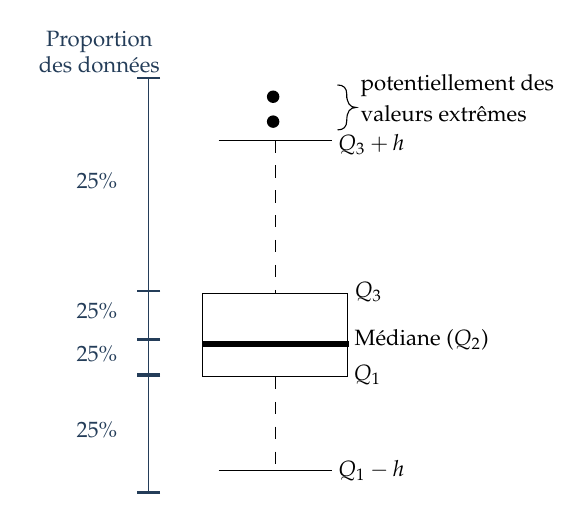
\begin{tikzpicture}[x=0.75pt,y=0.75pt,yscale=-1,xscale=1]
%uncomment if require: \path (0,300); %set diagram left start at 0, and has height of 300

%Straight Lines [id:da129737114081373] 
\draw  [dash pattern={on 4.5pt off 4.5pt}]  (181,70) -- (181,144) ;
%Straight Lines [id:da6241443915481115] 
\draw  [dash pattern={on 4.5pt off 4.5pt}]  (181,184) -- (181,229) ;
%Shape: Rectangle [id:dp9646011782302748] 
\draw   (146,144) -- (216,144) -- (216,184) -- (146,184) -- cycle ;
%Straight Lines [id:da9057676058861892] 
\draw    (153.75,229) -- (208.25,229) ;
%Straight Lines [id:da28703820276341374] 
\draw    (153.75,70) -- (208.25,70) ;
%Straight Lines [id:da23169419071689368] 
\draw [line width=2.25]    (145.75,168) -- (216.5,168) ;
%Shape: Circle [id:dp21208293035447068] 
\draw  [draw opacity=0][fill={rgb, 255:red, 0; green, 0; blue, 0 }  ,fill opacity=1 ] (177,61) .. controls (177,59.34) and (178.34,58) .. (180,58) .. controls (181.66,58) and (183,59.34) .. (183,61) .. controls (183,62.66) and (181.66,64) .. (180,64) .. controls (178.34,64) and (177,62.66) .. (177,61) -- cycle ;
%Shape: Circle [id:dp06804994911291695] 
\draw  [draw opacity=0][fill={rgb, 255:red, 0; green, 0; blue, 0 }  ,fill opacity=1 ] (177,49) .. controls (177,47.34) and (178.34,46) .. (180,46) .. controls (181.66,46) and (183,47.34) .. (183,49) .. controls (183,50.66) and (181.66,52) .. (180,52) .. controls (178.34,52) and (177,50.66) .. (177,49) -- cycle ;
%Shape: Brace [id:dp16337358256224843] 
\draw   (211,65) .. controls (213.97,65) and (215.46,63.51) .. (215.46,60.54) -- (215.46,60.54) .. controls (215.46,56.29) and (216.95,54.17) .. (219.92,54.17) .. controls (216.95,54.17) and (215.46,52.04) .. (215.46,47.79)(215.46,49.71) -- (215.46,47.79) .. controls (215.46,44.82) and (213.97,43.33) .. (211,43.33) ;
%Straight Lines [id:da0690372797278489] 
\draw [color={rgb, 255:red, 36; green, 61; blue, 89 }  ,draw opacity=1 ]   (120,40) -- (120,142.67) ;
\draw [shift={(120,142.67)}, rotate = 270] [color={rgb, 255:red, 36; green, 61; blue, 89 }  ,draw opacity=1 ][line width=0.75]    (0,5.59) -- (0,-5.59)   ;
\draw [shift={(120,40)}, rotate = 270] [color={rgb, 255:red, 36; green, 61; blue, 89 }  ,draw opacity=1 ][line width=0.75]    (0,5.59) -- (0,-5.59)   ;
%Straight Lines [id:da0032989468420259183] 
\draw [color={rgb, 255:red, 36; green, 61; blue, 89 }  ,draw opacity=1 ]   (120,142.67) -- (120,165.67) ;
\draw [shift={(120,165.67)}, rotate = 270] [color={rgb, 255:red, 36; green, 61; blue, 89 }  ,draw opacity=1 ][line width=0.75]    (0,5.59) -- (0,-5.59)   ;
\draw [shift={(120,142.67)}, rotate = 270] [color={rgb, 255:red, 36; green, 61; blue, 89 }  ,draw opacity=1 ][line width=0.75]    (0,5.59) -- (0,-5.59)   ;
%Straight Lines [id:da7171607128941915] 
\draw [color={rgb, 255:red, 36; green, 61; blue, 89 }  ,draw opacity=1 ]   (120,166.33) -- (120,183.33) ;
\draw [shift={(120,183.33)}, rotate = 270] [color={rgb, 255:red, 36; green, 61; blue, 89 }  ,draw opacity=1 ][line width=0.75]    (0,5.59) -- (0,-5.59)   ;
\draw [shift={(120,166.33)}, rotate = 270] [color={rgb, 255:red, 36; green, 61; blue, 89 }  ,draw opacity=1 ][line width=0.75]    (0,5.59) -- (0,-5.59)   ;
%Straight Lines [id:da8789207501910292] 
\draw [color={rgb, 255:red, 36; green, 61; blue, 89 }  ,draw opacity=1 ]   (120,182.67) -- (120,239.67) ;
\draw [shift={(120,239.67)}, rotate = 270] [color={rgb, 255:red, 36; green, 61; blue, 89 }  ,draw opacity=1 ][line width=0.75]    (0,5.59) -- (0,-5.59)   ;
\draw [shift={(120,182.67)}, rotate = 270] [color={rgb, 255:red, 36; green, 61; blue, 89 }  ,draw opacity=1 ][line width=0.75]    (0,5.59) -- (0,-5.59)   ;

% Text Node
\draw (221,37) node [anchor=north west][inner sep=0.75pt] [font=\footnotesize]  [align=left] {
\shortstack[l]{potentiellement des\\ valeurs extrêmes}};
% Text Node
\draw (218,137) node [anchor=north west][inner sep=0.75pt]  [font=\footnotesize] [align=left] {$\displaystyle Q_{3}$};
% Text Node
\draw (217.5,177) node [anchor=north west][inner sep=0.75pt]  [font=\footnotesize] [align=left] {$\displaystyle Q_{1}$};
% Text Node
\draw (218,160) node [anchor=north west][inner sep=0.75pt]  [font=\footnotesize] [align=left] {Médiane ($\displaystyle Q_{2}$)};
% Text Node
\draw (62,16) node [anchor=north west][inner sep=0.75pt]  [font=\footnotesize,color={rgb, 255:red, 36; green, 61; blue, 89 }  ,opacity=1 ] [align=left] {\begin{minipage}[lt]{49.455856000000004pt}\setlength\topsep{0pt}
\begin{center}
Proportion \\des données
\end{center}
\end{minipage}};
% Text Node
\draw (84,84.33) node [anchor=north west][inner sep=0.75pt]  [font=\footnotesize,color={rgb, 255:red, 36; green, 61; blue, 89 }  ,opacity=1 ] [align=left] {$\displaystyle 25\%$};
% Text Node
\draw (84,147.17) node [anchor=north west][inner sep=0.75pt]  [font=\footnotesize,color={rgb, 255:red, 36; green, 61; blue, 89 }  ,opacity=1 ] [align=left] {$\displaystyle 25\%$};
% Text Node
\draw (84,167.83) node [anchor=north west][inner sep=0.75pt]  [font=\footnotesize,color={rgb, 255:red, 36; green, 61; blue, 89 }  ,opacity=1 ] [align=left] {$\displaystyle 25\%$};
% Text Node
\draw (84,204.17) node [anchor=north west][inner sep=0.75pt]  [font=\footnotesize,color={rgb, 255:red, 36; green, 61; blue, 89 }  ,opacity=1 ] [align=left] {$\displaystyle 25\%$};
% Text Node
\draw (210,66) node [anchor=north west][inner sep=0.75pt]  [font=\footnotesize] [align=left] {$\displaystyle Q_{3} +h$};
% Text Node
\draw (210,223) node [anchor=north west][inner sep=0.75pt]  [font=\footnotesize] [align=left] {$\displaystyle Q_{1} -h$};
\end{tikzpicture}
\end{center}

\begin{itemize}
	\item	La médiane est la ligne contenu dans la boîte.
		\begin{itemize}
		\item	La moitié des données sont au-dessus, et l'autre moitié en-dessous, de la ligne.
		\end{itemize}
	\item	La boîte est délimitée par le premier et le troisième quartile.
		\begin{itemize}
		\item	Il s'ensuit que la boîte contient la moitié des données.
		\item	De plus, 25\% des données sont contenues entre la borne \textit{supérieure} de la boîte et la médiane avec l'autre 25\% qui est contenu entre la borne \textit{inférieure} et la médiane.
		\end{itemize}
	\item	Les « moustaches » de la boîte sont tracées à un pas $h$ des quartiles où \lfbox[conditions]{$h = 1.5 \cdot (Q_{3} - Q_{1})$}.
		\begin{itemize}
		\item	Les points qui sont à l'extérieur de ces bornes sont les données potentiellement aberrantes.
		\item	$Q_{3}	-	Q_{1}$ correspond à l'écart interquartile.
		\item	Plus l'écart est élevé, plus la boîte sera large et, par conséquent, plus les moustaches seront situées loin de la médiane.
		\item	Le 1.5 est basé sur la règle du 68-95-99.7 avec moins de 1\% des données à l'extérieur de la borne supérieure.
		\end{itemize}
\end{itemize}

\begin{definitionNOHFILLprop}[Règle du 68-95-99.7]
Pour une distribution normale, environ 68\% des données sont en dedans d'un écart-type de la moyenne, 95\% en dedans de 2 et 99.7\% en dedans de 3.

\begin{center}
		
\tikzset{every picture/.style={line width=0.75pt}} %set default line width to 0.75pt        

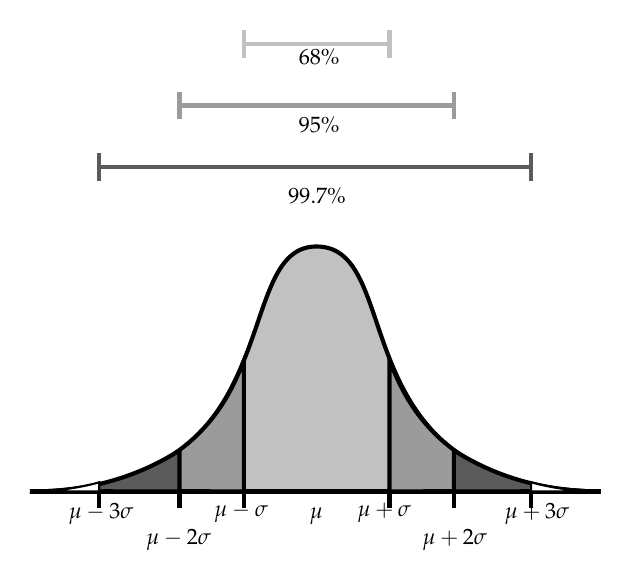
\begin{tikzpicture}[x=0.75pt,y=0.75pt,yscale=-1,xscale=1]
%uncomment if require: \path (0,278); %set diagram left start at 0, and has height of 278

%Curve Lines [id:da8749420139531441] 
\draw [draw opacity=0][fill={rgb, 255:red, 193; green, 193; blue, 193 }  ,fill opacity=1 ][line width=1.5]    (389,225.7) .. controls (520.68,226.75) and (483.98,107.66) .. (527.13,107.66) .. controls (571.77,107.66) and (537.05,225.26) .. (664.02,225.7) ;
%Straight Lines [id:da8888686520092737] 
\draw [line width=1.5]    (422.48,225.7) -- (422.48,233.64) ;
%Straight Lines [id:da1699364296805208] 
\draw [line width=1.5]    (593.34,225.7) -- (593.34,233.64) ;
%Curve Lines [id:da41861109546010566] 
\draw [line width=1.5]    (389,225.7) .. controls (517.71,227.49) and (483.98,107.66) .. (527.13,107.66) .. controls (571.77,107.66) and (536.06,225.21) .. (664.02,225.7) ;
%Straight Lines [id:da8400965165974321] 
\draw [line width=1.5]    (389,225.7) -- (664.02,225.7) ;
%Shape: Regular Polygon [id:dp11998667280876218] 
\draw  [fill={rgb, 255:red, 155; green, 155; blue, 155 }  ,fill opacity=1 ][line width=1.5]  (664.02,225.7) .. controls (584.29,225.26) and (568.2,176.16) .. (562.34,162.77) .. controls (562.34,225.26) and (562.34,162.77) .. (562.34,225.7) .. controls (663.29,225.26) and (562.34,225.26) .. (664.02,225.7) -- cycle ;
%Shape: Regular Polygon [id:dp898895201503896] 
\draw  [fill={rgb, 255:red, 155; green, 155; blue, 155 }  ,fill opacity=1 ][line width=1.5]  (390.49,225.7) .. controls (470.22,225.26) and (486.31,176.16) .. (492.16,162.77) .. controls (492.16,225.26) and (492.16,162.77) .. (492.16,225.7) .. controls (391.22,225.26) and (492.16,225.26) .. (390.49,225.7) -- cycle ;
%Shape: Regular Polygon [id:dp6032696284614307] 
\draw  [fill={rgb, 255:red, 91; green, 91; blue, 91 }  ,fill opacity=1 ][line width=1.5]  (391.98,225.7) .. controls (426.94,225.26) and (449.26,213.36) .. (461.16,205.92) .. controls (461.16,225.26) and (461.16,205.92) .. (461.16,225.7) .. controls (392.47,225.58) and (461.16,225.58) .. (391.98,225.7) -- cycle ;
%Shape: Regular Polygon [id:dp8816872519073748] 
\draw  [fill={rgb, 255:red, 91; green, 91; blue, 91 }  ,fill opacity=1 ][line width=1.5]  (662.53,225.7) .. controls (627.57,225.26) and (605.25,213.36) .. (593.34,205.92) .. controls (593.34,225.26) and (593.34,205.92) .. (593.34,225.7) .. controls (662.03,225.58) and (593.34,225.58) .. (662.53,225.7) -- cycle ;
%Shape: Polygon Curved [id:ds6677084709851981] 
\draw  [fill={rgb, 255:red, 255; green, 255; blue, 255 }  ,fill opacity=1 ][line width=0.75]  (391.98,225.7) .. controls (403.14,225.7) and (417.23,222.92) .. (422.48,221.24) .. controls (422.48,225.6) and (422.48,221.24) .. (422.48,225.7) .. controls (392.2,225.67) and (422.48,225.7) .. (391.98,225.7) -- cycle ;
%Shape: Regular Polygon [id:dp8410749943461926] 
\draw  [fill={rgb, 255:red, 255; green, 255; blue, 255 }  ,fill opacity=1 ][line width=0.75]  (661.04,225.7) .. controls (649.88,225.7) and (635.79,222.92) .. (630.54,221.24) .. controls (630.54,225.6) and (630.54,221.24) .. (630.54,225.7) .. controls (660.82,225.67) and (630.54,225.7) .. (661.04,225.7) -- cycle ;
%Straight Lines [id:da38668537998939256] 
\draw [line width=1.5]    (461.16,225.7) -- (461.16,233.64) ;
%Straight Lines [id:da1998162556500347] 
\draw [line width=1.5]    (492.16,225.7) -- (492.16,233.64) ;
%Straight Lines [id:da12951125252628293] 
\draw [line width=1.5]    (562.34,225.7) -- (562.34,233.64) ;
%Straight Lines [id:da4432220170088057] 
\draw [line width=1.5]    (630.54,225.7) -- (630.54,233.64) ;
%Straight Lines [id:da9928263828524586] 
\draw [color={rgb, 255:red, 193; green, 193; blue, 193 }  ,draw opacity=1 ][line width=1.5]    (562.34,9.95) -- (492.16,9.95) ;
\draw [shift={(492.16,9.95)}, rotate = 360] [color={rgb, 255:red, 193; green, 193; blue, 193 }  ,draw opacity=1 ][line width=1.5]    (0,6.71) -- (0,-6.71)   ;
\draw [shift={(562.34,9.95)}, rotate = 360] [color={rgb, 255:red, 193; green, 193; blue, 193 }  ,draw opacity=1 ][line width=1.5]    (0,6.71) -- (0,-6.71)   ;
%Straight Lines [id:da37156360440094294] 
\draw [color={rgb, 255:red, 155; green, 155; blue, 155 }  ,draw opacity=1 ][line width=1.5]    (593.34,39.71) -- (461.16,39.71) ;
\draw [shift={(461.16,39.71)}, rotate = 360] [color={rgb, 255:red, 155; green, 155; blue, 155 }  ,draw opacity=1 ][line width=1.5]    (0,6.71) -- (0,-6.71)   ;
\draw [shift={(593.34,39.71)}, rotate = 360] [color={rgb, 255:red, 155; green, 155; blue, 155 }  ,draw opacity=1 ][line width=1.5]    (0,6.71) -- (0,-6.71)   ;
%Straight Lines [id:da8337470834507461] 
\draw [color={rgb, 255:red, 91; green, 91; blue, 91 }  ,draw opacity=1 ][line width=1.5]    (630.54,69.47) -- (422.48,69.47) ;
\draw [shift={(422.48,69.47)}, rotate = 360] [color={rgb, 255:red, 91; green, 91; blue, 91 }  ,draw opacity=1 ][line width=1.5]    (0,6.71) -- (0,-6.71)   ;
\draw [shift={(630.54,69.47)}, rotate = 360] [color={rgb, 255:red, 91; green, 91; blue, 91 }  ,draw opacity=1 ][line width=1.5]    (0,6.71) -- (0,-6.71)   ;

% Text Node
\draw (522.62,232.23) node [anchor=north west][inner sep=0.75pt]   [align=left] {{\footnotesize $\displaystyle \mu $}};
% Text Node
\draw (545.6,230.23) node [anchor=north west][inner sep=0.75pt]   [align=left] {{\footnotesize $\displaystyle \mu +\sigma $}};
% Text Node
\draw (576.84,242.62) node [anchor=north west][inner sep=0.75pt]  [font=\normalsize] [align=left] {{\footnotesize $\displaystyle \mu +2\sigma $}};
% Text Node
\draw (616.5,230.23) node [anchor=north west][inner sep=0.75pt]   [align=left] {{\footnotesize $\displaystyle \mu +3\sigma $}};
% Text Node
\draw (517.35,11.12) node [anchor=north west][inner sep=0.75pt]   [align=left] {{\footnotesize 68\%}};
% Text Node
\draw (517.35,43.86) node [anchor=north west][inner sep=0.75pt]   [align=left] {{\footnotesize 95\%}};
% Text Node
\draw (512.35,78.08) node [anchor=north west][inner sep=0.75pt]   [align=left] {{\footnotesize 99.7\%}};
% Text Node
\draw (476.6,230.23) node [anchor=north west][inner sep=0.75pt]   [align=left] {{\footnotesize $\displaystyle \mu -\sigma $}};
% Text Node
\draw (443.84,242.62) node [anchor=north west][inner sep=0.75pt]  [font=\normalsize] [align=left] {{\footnotesize $\displaystyle \mu -2\sigma $}};
% Text Node
\draw (406.5,230.23) node [anchor=north west][inner sep=0.75pt]   [align=left] {{\footnotesize $\displaystyle \mu -3\sigma $}};
\end{tikzpicture}

\end{center}
\end{definitionNOHFILLprop}

\columnbreak
En bref, le diagramme en boîte permet d'évaluer comment les données sont distribuées. Cette image de \href{https://en.wikipedia.org/wiki/Interquartile_range}{wikipedia} résume bien : 
\begin{center}
	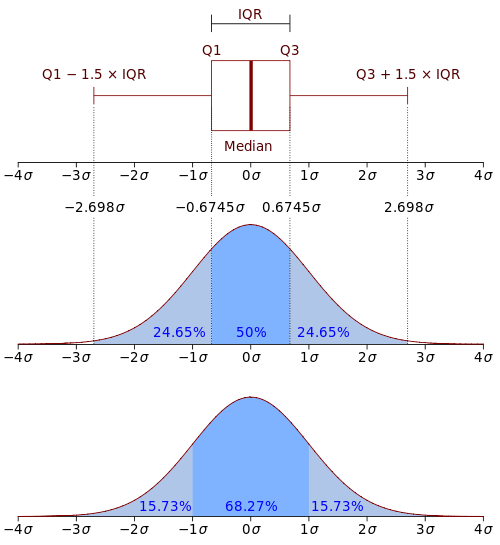
\includegraphics[scale=0.4]{../../src/ACT-2000/boxplot-normrule.png}
\end{center}


\columnbreak
\subsubsection{Diagramme quantile-quantile (\og \textit{Q-Q plot} \fg{})}
En pratique, on pose souvent que les données suivent une distribution. Un diagramme quantile-quantile permet de comparer les quantiles théoriques de la distribution aux quantiles empiriques des données. \\

Dans un tel cas, on connait la distribution, mais pas les paramètres.
\begin{itemize}
	\item	Si les données sont normalement distribuées, on peut centrer et réduire pour obtenir la loi normale standard $Z$ ; 
		\begin{itemize}
		\item	Ceci correspond à un diagramme quantile-quantile \textbf{normale} ;
		\end{itemize}
	\item	Autrement, le diagramme quantile-quantile est tracé en estimant les paramètres de la distribution avec l'échantillon de données.
\end{itemize}

\

Par exemple :
\begin{center}
\tikzset{every picture/.style={line width=0.75pt}} %set default line width to 0.75pt        

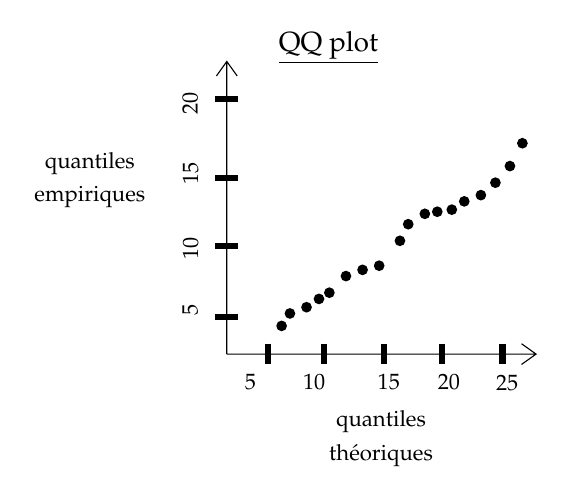
\begin{tikzpicture}[x=0.75pt,y=0.75pt,yscale=-1,xscale=1]
%uncomment if require: \path (0,300); %set diagram left start at 0, and has height of 300

%Shape: Axis 2D [id:dp6907328462183413] 
\draw  (159.17,162) -- (308.17,162)(159.17,21) -- (159.17,162) -- cycle (301.17,157) -- (308.17,162) -- (301.17,167) (154.17,28) -- (159.17,21) -- (164.17,28)  ;
%Straight Lines [id:da2684391209424455] 
\draw [line width=2.25]    (179,157) -- (179,167) ;
%Straight Lines [id:da26665731526815106] 
\draw [line width=2.25]    (206,157) -- (206,167) ;
%Straight Lines [id:da5458795480754546] 
\draw [line width=2.25]    (235,157) -- (235,167) ;
%Straight Lines [id:da7749608799910399] 
\draw [line width=2.25]    (263,157) -- (263,167) ;
%Straight Lines [id:da781366529806411] 
\draw [line width=2.25]    (292,157) -- (292,167) ;
%Straight Lines [id:da5656665110363344] 
\draw [line width=2.25]    (153.67,39) -- (164.5,39) ;
%Straight Lines [id:da06457141428798874] 
\draw [line width=2.25]    (153.67,77) -- (164.5,77) ;
%Straight Lines [id:da07440013590512717] 
\draw [line width=2.25]    (153.67,110) -- (164.5,110) ;
%Straight Lines [id:da7046117446976516] 
\draw [line width=2.25]    (153.67,144) -- (164.5,144) ;
%Flowchart: Connector [id:dp26709638677620307] 
\draw  [draw opacity=0][fill={rgb, 255:red, 0; green, 0; blue, 0 }  ,fill opacity=1 ] (187,142.42) .. controls (187,140.99) and (188.16,139.83) .. (189.58,139.83) .. controls (191.01,139.83) and (192.17,140.99) .. (192.17,142.42) .. controls (192.17,143.84) and (191.01,145) .. (189.58,145) .. controls (188.16,145) and (187,143.84) .. (187,142.42) -- cycle ;
%Flowchart: Connector [id:dp9807914547061263] 
\draw  [draw opacity=0][fill={rgb, 255:red, 0; green, 0; blue, 0 }  ,fill opacity=1 ] (183,148.42) .. controls (183,146.99) and (184.16,145.83) .. (185.58,145.83) .. controls (187.01,145.83) and (188.17,146.99) .. (188.17,148.42) .. controls (188.17,149.84) and (187.01,151) .. (185.58,151) .. controls (184.16,151) and (183,149.84) .. (183,148.42) -- cycle ;
%Flowchart: Connector [id:dp15148611073322638] 
\draw  [draw opacity=0][fill={rgb, 255:red, 0; green, 0; blue, 0 }  ,fill opacity=1 ] (195,139.42) .. controls (195,137.99) and (196.16,136.83) .. (197.58,136.83) .. controls (199.01,136.83) and (200.17,137.99) .. (200.17,139.42) .. controls (200.17,140.84) and (199.01,142) .. (197.58,142) .. controls (196.16,142) and (195,140.84) .. (195,139.42) -- cycle ;
%Flowchart: Connector [id:dp8718571676300524] 
\draw  [draw opacity=0][fill={rgb, 255:red, 0; green, 0; blue, 0 }  ,fill opacity=1 ] (201,135.42) .. controls (201,133.99) and (202.16,132.83) .. (203.58,132.83) .. controls (205.01,132.83) and (206.17,133.99) .. (206.17,135.42) .. controls (206.17,136.84) and (205.01,138) .. (203.58,138) .. controls (202.16,138) and (201,136.84) .. (201,135.42) -- cycle ;
%Flowchart: Connector [id:dp6298382695689162] 
\draw  [draw opacity=0][fill={rgb, 255:red, 0; green, 0; blue, 0 }  ,fill opacity=1 ] (206,132.42) .. controls (206,130.99) and (207.16,129.83) .. (208.58,129.83) .. controls (210.01,129.83) and (211.17,130.99) .. (211.17,132.42) .. controls (211.17,133.84) and (210.01,135) .. (208.58,135) .. controls (207.16,135) and (206,133.84) .. (206,132.42) -- cycle ;
%Flowchart: Connector [id:dp7974400157875505] 
\draw  [draw opacity=0][fill={rgb, 255:red, 0; green, 0; blue, 0 }  ,fill opacity=1 ] (214,124.42) .. controls (214,122.99) and (215.16,121.83) .. (216.58,121.83) .. controls (218.01,121.83) and (219.17,122.99) .. (219.17,124.42) .. controls (219.17,125.84) and (218.01,127) .. (216.58,127) .. controls (215.16,127) and (214,125.84) .. (214,124.42) -- cycle ;
%Flowchart: Connector [id:dp18385794853649817] 
\draw  [draw opacity=0][fill={rgb, 255:red, 0; green, 0; blue, 0 }  ,fill opacity=1 ] (222,121.42) .. controls (222,119.99) and (223.16,118.83) .. (224.58,118.83) .. controls (226.01,118.83) and (227.17,119.99) .. (227.17,121.42) .. controls (227.17,122.84) and (226.01,124) .. (224.58,124) .. controls (223.16,124) and (222,122.84) .. (222,121.42) -- cycle ;
%Flowchart: Connector [id:dp41038901090251567] 
\draw  [draw opacity=0][fill={rgb, 255:red, 0; green, 0; blue, 0 }  ,fill opacity=1 ] (230,119.42) .. controls (230,117.99) and (231.16,116.83) .. (232.58,116.83) .. controls (234.01,116.83) and (235.17,117.99) .. (235.17,119.42) .. controls (235.17,120.84) and (234.01,122) .. (232.58,122) .. controls (231.16,122) and (230,120.84) .. (230,119.42) -- cycle ;
%Flowchart: Connector [id:dp9668794505330132] 
\draw  [draw opacity=0][fill={rgb, 255:red, 0; green, 0; blue, 0 }  ,fill opacity=1 ] (240,107.42) .. controls (240,105.99) and (241.16,104.83) .. (242.58,104.83) .. controls (244.01,104.83) and (245.17,105.99) .. (245.17,107.42) .. controls (245.17,108.84) and (244.01,110) .. (242.58,110) .. controls (241.16,110) and (240,108.84) .. (240,107.42) -- cycle ;
%Flowchart: Connector [id:dp23760159423012994] 
\draw  [draw opacity=0][fill={rgb, 255:red, 0; green, 0; blue, 0 }  ,fill opacity=1 ] (244,99.42) .. controls (244,97.99) and (245.16,96.83) .. (246.58,96.83) .. controls (248.01,96.83) and (249.17,97.99) .. (249.17,99.42) .. controls (249.17,100.84) and (248.01,102) .. (246.58,102) .. controls (245.16,102) and (244,100.84) .. (244,99.42) -- cycle ;
%Flowchart: Connector [id:dp9760550495862494] 
\draw  [draw opacity=0][fill={rgb, 255:red, 0; green, 0; blue, 0 }  ,fill opacity=1 ] (252,94.42) .. controls (252,92.99) and (253.16,91.83) .. (254.58,91.83) .. controls (256.01,91.83) and (257.17,92.99) .. (257.17,94.42) .. controls (257.17,95.84) and (256.01,97) .. (254.58,97) .. controls (253.16,97) and (252,95.84) .. (252,94.42) -- cycle ;
%Flowchart: Connector [id:dp09806905504709196] 
\draw  [draw opacity=0][fill={rgb, 255:red, 0; green, 0; blue, 0 }  ,fill opacity=1 ] (258,93.42) .. controls (258,91.99) and (259.16,90.83) .. (260.58,90.83) .. controls (262.01,90.83) and (263.17,91.99) .. (263.17,93.42) .. controls (263.17,94.84) and (262.01,96) .. (260.58,96) .. controls (259.16,96) and (258,94.84) .. (258,93.42) -- cycle ;
%Flowchart: Connector [id:dp21547983210697952] 
\draw  [draw opacity=0][fill={rgb, 255:red, 0; green, 0; blue, 0 }  ,fill opacity=1 ] (265,92.42) .. controls (265,90.99) and (266.16,89.83) .. (267.58,89.83) .. controls (269.01,89.83) and (270.17,90.99) .. (270.17,92.42) .. controls (270.17,93.84) and (269.01,95) .. (267.58,95) .. controls (266.16,95) and (265,93.84) .. (265,92.42) -- cycle ;
%Flowchart: Connector [id:dp13436174967362358] 
\draw  [draw opacity=0][fill={rgb, 255:red, 0; green, 0; blue, 0 }  ,fill opacity=1 ] (271,88.42) .. controls (271,86.99) and (272.16,85.83) .. (273.58,85.83) .. controls (275.01,85.83) and (276.17,86.99) .. (276.17,88.42) .. controls (276.17,89.84) and (275.01,91) .. (273.58,91) .. controls (272.16,91) and (271,89.84) .. (271,88.42) -- cycle ;
%Flowchart: Connector [id:dp6321990138892946] 
\draw  [draw opacity=0][fill={rgb, 255:red, 0; green, 0; blue, 0 }  ,fill opacity=1 ] (279,85.42) .. controls (279,83.99) and (280.16,82.83) .. (281.58,82.83) .. controls (283.01,82.83) and (284.17,83.99) .. (284.17,85.42) .. controls (284.17,86.84) and (283.01,88) .. (281.58,88) .. controls (280.16,88) and (279,86.84) .. (279,85.42) -- cycle ;
%Flowchart: Connector [id:dp8650742018499089] 
\draw  [draw opacity=0][fill={rgb, 255:red, 0; green, 0; blue, 0 }  ,fill opacity=1 ] (286,79.42) .. controls (286,77.99) and (287.16,76.83) .. (288.58,76.83) .. controls (290.01,76.83) and (291.17,77.99) .. (291.17,79.42) .. controls (291.17,80.84) and (290.01,82) .. (288.58,82) .. controls (287.16,82) and (286,80.84) .. (286,79.42) -- cycle ;
%Flowchart: Connector [id:dp8249100072120605] 
\draw  [draw opacity=0][fill={rgb, 255:red, 0; green, 0; blue, 0 }  ,fill opacity=1 ] (293,71.42) .. controls (293,69.99) and (294.16,68.83) .. (295.58,68.83) .. controls (297.01,68.83) and (298.17,69.99) .. (298.17,71.42) .. controls (298.17,72.84) and (297.01,74) .. (295.58,74) .. controls (294.16,74) and (293,72.84) .. (293,71.42) -- cycle ;
%Flowchart: Connector [id:dp5353454981608219] 
\draw  [draw opacity=0][fill={rgb, 255:red, 0; green, 0; blue, 0 }  ,fill opacity=1 ] (299,60.42) .. controls (299,58.99) and (300.16,57.83) .. (301.58,57.83) .. controls (303.01,57.83) and (304.17,58.99) .. (304.17,60.42) .. controls (304.17,61.84) and (303.01,63) .. (301.58,63) .. controls (300.16,63) and (299,61.84) .. (299,60.42) -- cycle ;


% Text Node
\draw (183,5) node [anchor=north west][inner sep=0.75pt]   [align=left] {\underline{QQ plot}};
% Text Node
\draw (205,188) node [anchor=north west][inner sep=0.75pt]   [align=left] {\begin{minipage}[lt]{40.828356pt}\setlength\topsep{0pt}
\begin{center}
{\footnotesize quantiles }\\{\footnotesize théoriques}
\end{center}

\end{minipage}};
% Text Node
\draw (63.5,63.5) node [anchor=north west][inner sep=0.75pt]   [align=left] {\begin{minipage}[lt]{42.634572pt}\setlength\topsep{0pt}
\begin{center}
{\footnotesize quantiles }\\{\footnotesize empiriques}
\end{center}

\end{minipage}};
% Text Node
\draw (166.62,170.3) node [anchor=north west][inner sep=0.75pt]  [font=\footnotesize] [align=left] {$\displaystyle 5$};
% Text Node
\draw (194.62,170.3) node [anchor=north west][inner sep=0.75pt]  [font=\footnotesize] [align=left] {$\displaystyle 10$};
% Text Node
\draw (230.62,170.3) node [anchor=north west][inner sep=0.75pt]  [font=\footnotesize] [align=left] {$\displaystyle 15$};
% Text Node
\draw (259.62,170.3) node [anchor=north west][inner sep=0.75pt]  [font=\footnotesize] [align=left] {$\displaystyle 20$};
% Text Node
\draw (287.62,170.8) node [anchor=north west][inner sep=0.75pt]  [font=\footnotesize] [align=left] {$\displaystyle 25$};
% Text Node
\draw (136.62,144.8) node [anchor=north west][inner sep=0.75pt]  [font=\footnotesize,rotate=-270] [align=left] {$\displaystyle 5$};
% Text Node
\draw (136.62,117.8) node [anchor=north west][inner sep=0.75pt]  [font=\footnotesize,rotate=-270] [align=left] {$\displaystyle 10$};
% Text Node
\draw (136.62,81.8) node [anchor=north west][inner sep=0.75pt]  [font=\footnotesize,rotate=-270] [align=left] {$\displaystyle 15$};
% Text Node
\draw (136.62,47.8) node [anchor=north west][inner sep=0.75pt]  [font=\footnotesize,rotate=-270] [align=left] {$\displaystyle 20$};
\end{tikzpicture}

\end{center}

Le diagramme quantile-quantile évalue si la distribution empirique est semblable à la distribution théorique. On peut, entre autre, évaluer la queue de la distribution. Selon la distribution, les quantiles « normaux » varient. Ci-dessous est une image de \href{https://mgimond.github.io/ES218/Week06a.html}{ce site} qui montre quantiles selon la distribution avec une droite pour la normale :
\begin{center}
	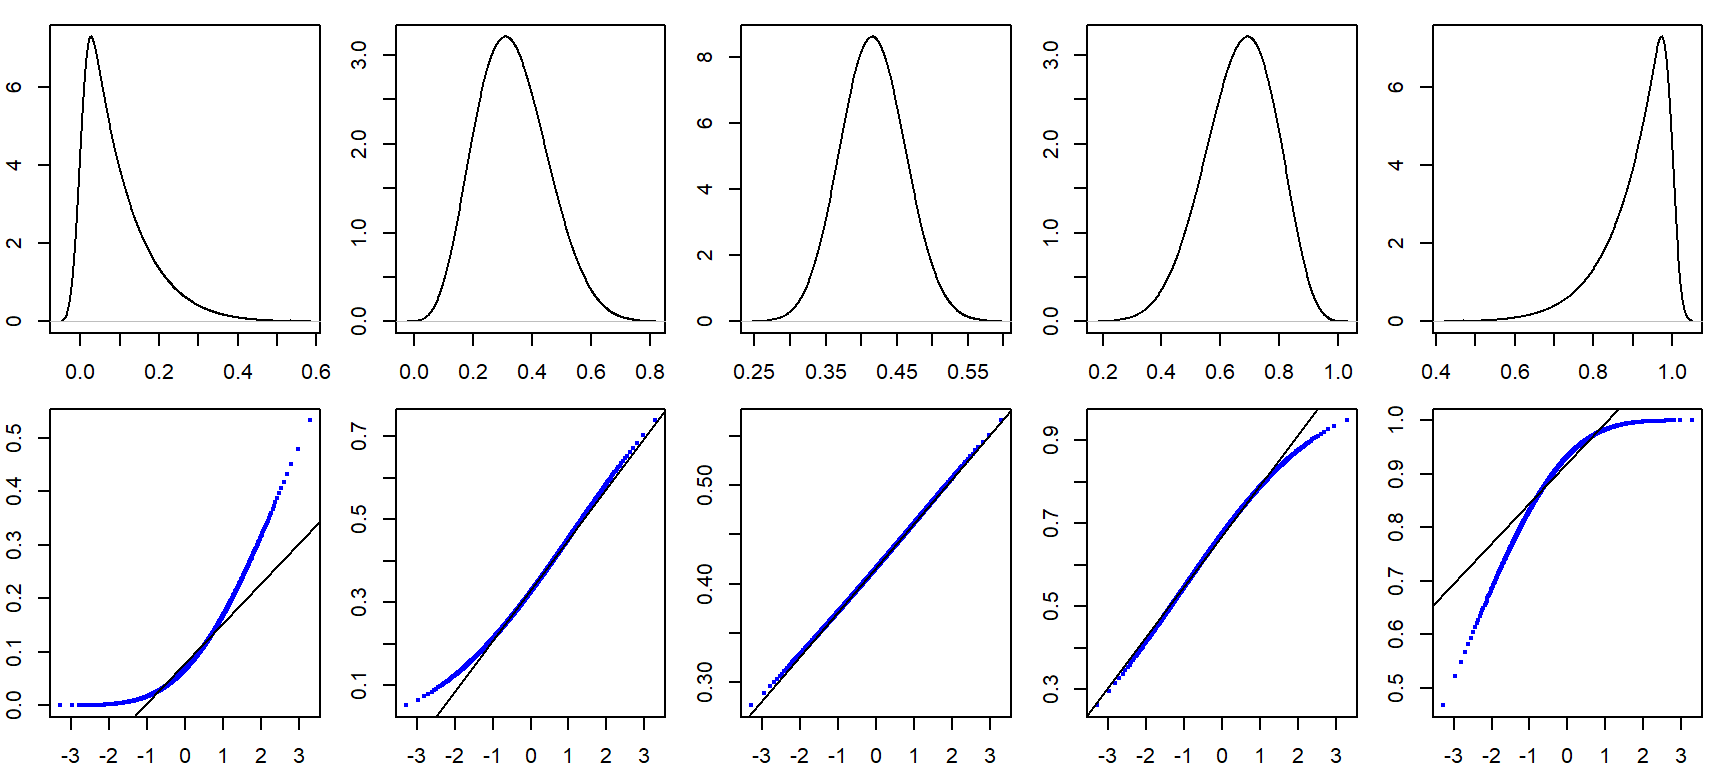
\includegraphics[scale=0.5]{../../src/ACT-2000/qqplot-skeweing.png}
\end{center}


\columnbreak
\section{Construction d'estimateurs}

Précédemment, nous avons décrit les méthodes utilisées pour évaluer la \textbf{qualité} de l'estimateur. 
Cependant, comment obtenons-nous des estimateurs à évaluer?

Plusieurs méthodes existent pour établir des estimateurs, de plus plusieurs méthodes existent pour estimer des paramètres.
La méthode vu dans le cadre du cours de statistique est la \textbf{méthode fréquentiste}, le cours de mathématiques IARD 1 (ACT-2005) présente \textbf{l'estimation bayésienne}.

Avant de le faire, nous présentons quelques concepts:
\begin{distributions}[Terminologie]
\begin{description}
	\item[$\mu_{k}'(\hat{\theta})$]	$k^{\text{e}}$ moment centré à 0, \icbox{$\mu_{k}' = \text{E}[X^{k}]$};
	\item[$\pi_{g}(\theta)$]	$100g^{\text{e}}$ pourcentile, \icbox{$\pi_{g}(\theta) = F^{-1}_{\theta}(g)$}, \icbox[red][palechestnut]{$g \in [0, 1]$};
	\item[$F_{e}(x)$]	Fonction de répartition \textbf{e}mpirique;
	\item[]	$\equalhat$	Notation pour poser une égalité.
\end{description}
\end{distributions}

Les deux premiers estimateurs ci-dessous sont les plus faciles à obtenir, mais sont aussi les moins performants puisqu'ils n'utilisent que quelques traits des données au lieu de l'entièreté des données comme la troisième méthode.

Cette distinction devient particulièrement importante dans le cas d'une distribution avec une queue lourde à la droite (Pareto, Weibull, etc.) où il devient plus essentiel de connaître les valeurs extrêmes pour bien estimer le paramètre de forme ($\alpha$ pour une Pareto).

Un autre désavantage est que les deux premières méthodes nécessitent que les données proviennent toutes de la même distribution. Sinon, les moments et quantiles ne seraient pas clairs.

Finalement, sous les deux premières méthodes la décision de quels moments et percentiles à utiliser est arbitraire.

\subsection{Méthode des moments (MoM)}

\begin{algo}{Estimation de $\theta$ par la méthode des moments}
Pour ajuster une distribution de $p$ paramètres, on pose égale les $p$ premiers moments empiriques $\hat\mu_{k}'$ au $p$ premiers moments de la distribution $\mu_{k}'$.\\
L'estimation de $\theta$ est alors toute solution des $p$ équations:
\begin{equation*}
	\hat{\mu}_{k}' 
	=	\frac{1}{n}\sum_{i = 1}^{n} x_{i}^{k}
	\equalhat	\esp{X^{k}}
	=	\mu_{k}'(\theta), \quad	k = 1, 2, \dots, p
\end{equation*}
\end{algo}

La raison pour cet estimateur est que la distribution empirique aura les mêmes $p$ premiers moments centrés à 0 que la distribution paramétrique.

\subsection{Méthode du \guillemotleft Percentile Matching \guillemotright}

\begin{algo}{Estimation de $\theta$ par la méthode du \og \textit{Percentile Matching} \fg{}}
Pour ajuster une distribution de $p$ paramètres, on pose égale $p$ pourcentiles $\hat{\pi}_{g}(\hat{\theta})$ de l'échantillon à ceux de la distribution $\pi_{g}(\theta)$.\\
L'estimation de $\theta$ est alors toute solution des $p$ équations:
\begin{equation*}
	F_{e}(\hat\pi_{g_{k}} | \theta)	=	g_{k}, \quad	k = 1, 2, \dots, p
\end{equation*}
\end{algo}

La raison pour cet estimateur est que le modèle produit aura $p$ percentiles qui vont \og \textit{matcher} \fg{} les données.

Il peut arriver que les percentiles de distributions ne soient pas uniques, par exemple dans le cas de données discrètes lorsque le quantile recherché peut tomber entre 2 \emph{marches} de la fonction empirique, ou mal-définis.
Il est alors utile de définir une méthode d'interpolation des quantiles (bien qu'il n'en existe pas une d'officielle).

Soit le \og \textit{smoothed empirical estimate} \fg{} d'un pourcentile:

\begin{algo}{Smoothed empirical estimate}
On utilise les statistiques d'ordre de l'échantillon $x_{(1)} \le x_{(2)} \le \dots \le x_{(n)}$ pour l'\textbf{interpolation} suivant:
\begin{align*}
	\hat\pi_{g}
	&=	(1 - h)x_{(j)} + h x_{(j + 1)}, \quad \text{ où }	\\
	j
	&=	\lfloor (n + 1) g \rfloor	\quad
	\text{ et }	\quad
	h
	=	(n + 1) g - j
\end{align*}
\end{algo}


\columnbreak
\subsection{Méthode du maximum de vraisemblance}

Nous cherchons à maximiser la probabilité d'observer les données.
Ceci est fait par la vraisemblance $\mathcal{L}(\theta; \bm{x})$ ou, puisque le logarithme ne change pas le maximum, la log-vraisemblance $\ell(\theta; x)$ où:

\begin{algo}{Maximum de vraisemblance}
\begin{align*}
	\mathcal{L}(\theta; \bm{x})
	&=	\prod_{i = 1}^{n}	f(x_{i}; \theta)	&
	&\text{et}	&
	\ell(\theta; \bm{x})
	&=	\sum_{i = 1}^{n} \ln	f(x_{i}; \theta)	&
\end{align*}
et l'\textbf{estimateur du maximum de vraisemblance} de $\bm\theta$ est celui qui maximise la fonction de vraisemblance.
\end{algo}

De façon formelle, on dit que \lfbox[formula]{$\hat{\theta}^{\text{EMV}}	=	\underset{\theta}{\max}\{\mathcal{L}(\theta; \bm{x})\}	=	\underset{\theta}{\max}\{\ln\mathcal{L}(\theta; \bm{x})\}$.}

\subsubsection{Raccourcis}

Si la fonction de vraisemblance est de la forme :
\begin{itemize}
	\item	\lfbox[formula]{$\mathcal{L}(\gamma)	=	\gamma^{-a}\textrm{e}^{-b/\gamma}$} alors \lfbox[formula]{$\hat{\gamma}^{\text{MLE}}	=	\frac{b}{a}$}.
	\item	\lfbox[formula]{$\mathcal{L}(\lambda)	=	\lambda^{a}\textrm{e}^{-\lambda b}$} alors \lfbox[formula]{$\hat{\lambda}^{\text{MLE}}	=	\frac{a}{b}$}.
	\item	\lfbox[formula]{$\mathcal{L}(\theta)	=	\theta^{a}(1	-	\theta)^{b}$} then \lfbox[formula]{$\hat{\theta}^{\text{MLE}}	=	\frac{a}{a + b}$}.
\end{itemize}


\subsubsection{Propriétés}
\begin{definitionNOHFILL}[Propriété d'invariance]
Soit une fonction bijective $g(\cdot)$ et l'estimateur du maximum de vraisemblance (EMV) $\hat{\theta}^{\text{EMV}}$ de $\theta$.\\
Alors, selon la propriété d'invariance \lfbox[formula]{$g(\hat{\theta}^{\text{EMV}})$ est l'EMV de $g(\theta)$.}\\

L'EMV satisfait cette propriété.
\end{definitionNOHFILL}

\begin{definitionNOHFILL}[Convergence en distribution de l'EMV]
\textbf{Théorème}:	\lfbox[formula]{$\hat{\theta}^{\text{EMV}}	\approx	\mathcal{N}\left(0, \frac{1}{\bm{I}_{n}(\theta)}\right)$.}

\tcbline

Sous \hyperlink{reg_cond}{\color{blue!40!green!80!black}certaines conditions de régularité}, la distribution de $\sqrt{n}\left( \hat{\theta}	-	\theta \right)$ converge en distribution vers une distribution normale avec une moyenne nulle et une variance égale à la \hyperref[sec:cramer_rao]{\color{azure(colorwheel)}borne de Cramér-Rao}.
\begin{align*}
	\sqrt{n}\left( \hat{\theta}	-	\theta \right)
	&\overset{D}{\rightarrow}
	\mathcal{N}\left( 0, \frac{1}{\bm{I}_{n}(\theta)} \right)
\end{align*}

Ce qui implique:
\begin{enumerate}
	\item	$\hat{\theta}$ est \lfbox[imphl]{asymptotiquement sans biais.}
	\item	$\hat{\theta}$ est \lfbox[imphl]{\og \textit{consistent} \fg{}.}
	\item	$\hat{\theta}$ est \lfbox[imphl]{approximativement normalement distribué avec moyenne $\theta$ et} \lfbox[imphl]{variance $1/\bm{I}_{n}(\theta)$ pour des grands échantillons.}
	\item	$\hat{\theta}$ est \lfbox[imphl]{asymptotiquement efficace} puisque sa variance tend vers la borne Cramér-Rao.
\end{enumerate}
\end{definitionNOHFILL}
	
Souvent les professeurs ne montrent pas ces conditions puisqu'elles sont compliquées. Alors, ne vous en faites pas si vous ne les comprenez pas complètement.

\begin{definitionNOHFILLsub}[\hypertarget{reg_cond}{Conditions de régularité}]
\begin{description}
	\item[R0]	Les variables $X_{i}$ sont iid avec densité $f(x_{i}; \theta)$ pour $i	=	1, 2, \dots$.
	\item[R1]	Les fonctions de densité ont tous le même support pour tout $\theta$.
		\begin{itemize}
		\item	C'est-à-dire que le support de $X_{i}$ ne dépend pas de $\theta$;
		\item	C'est une condition restrictive que certains modèles ne respectent pas.
		\end{itemize}
	\item[R2]	La "vraie valeur" de $\theta$ est contenue dans l'ensemble des valeurs possibles $\Theta$.
\tcbline
\begin{description}
	\item[R3]	La fonction de densité $f(x; \theta)$ est différentiable deux fois comme fonction de $\theta$.
		\begin{itemize}
		\item	Cette condition additionnelle assure que les deux premières dérivées existent pour \hyperref[sec:cramer_rao]{\color{azure(colorwheel)}la borne de Cramér-Rao}.
		\end{itemize}
	\item[R4]	L'intégrale $\int f(x; \theta) dx$ est différentiable deux fois sous l'intégrale comme fonction de $\theta$.
		\begin{itemize}
		\item	Cette condition additionnelle assure que l'on peut utiliser la deuxième dérivée pour \hyperref[sec:cramer_rao]{\color{azure(colorwheel)}la borne de Cramér-Rao}.
		\end{itemize}
\end{description}
\end{description}
%%%	--------------------------------
%%%	NOTES:
%%%	+	FAUT AJOUTER DES DÉTAILS SUR LES CONDITIONS AVEC LES DÉRIVÉES D'INTÉGRALES ÉGAUX À ZÉRO!!!!!
%%%	+	Ajouter des détails sur l'efficacité asymptotique;
%%%	+	Intervalles de confiance
%%%	--------------------------------
%\begin{description}
%	\item[R5]	La fonction de densité $f(x; \theta)$ est différentiable trois fois comme fonction de $\theta$. De plus, $\forall \theta \in \Theta$ il existe une constante $c$ and une fonction $g(x)$ tel que $\big| \deriv[3]{\theta}{} \ln f(x; \theta) \big| \leq g(x)$.
%\end{description}
%%%	Impliquent que l'on peut interchanger l'intégration et la différention wrt/ \theta
\end{definitionNOHFILLsub}
	

\subsubsection{Cas multivarié}
On généralise du cas où $\theta$ est un scalaire (un seul paramètre) au cas multivarié avec $k$ paramètres et le vecteur $\bm{\theta}	=	(\theta_{1}, \cdots, \theta_{k})^{\top}$.\\


\begin{distributions}[Notation]
En notation matricielle, on multiple le vecteur $\bm{\theta}$ par la transposée $\bm{\theta}^{\top}$ au lieu de mettre $\theta$ au carré. 
\begin{itemize}
	\item	La matrice d'information Fisher \underline{d'\textit{une} observation} est donc une matrice $k \times k$:
\begin{align*}
	\bm{I}(\bm{\theta})
	&=	\text{E}\left[	
			\frac{\partial \ln f(X; \bm{\theta})}{\partial \bm{\theta}}
			\frac{\partial \ln f(X; \bm{\theta})}{\partial \bm{\theta}^{\top}}
		\right]
	\overset{iid}{=}	\text{E}\left[	
			\frac{\partial^{2} \ln f(X; \bm{\theta})}{\partial \bm{\theta}\bm{\theta}^{\top}}
		\right]
\end{align*}
%%%	------------------------
%%%	NOTES
%%%	+	Vérifier les X pour voir où les majuscules vont avec matrice d'information Fisher!!! vs f(x; \theta), f(X; \theta) ,,......\bm{X}?
%%%	------------------------
	\item	Pour la matrice d'information Fisher d'un échantillon aléatoire de $n$ observation, on utilise la relation $\bm{I}_{n}(\bm{\theta})	=	n\bm{I}(\bm{\theta})$.
\end{itemize}
\begin{description}
	\item[$\bm{I}^{-1}_{n}(\bm{\theta})$]	Inverse de la matrice d'information Fisher $\bm{I}_{n}(\bm{\theta})$.
\end{description}
\end{distributions}

Soit $\tilde{\bm{\theta}}$ un estimateur sans bais de $\bm{\theta}$. 

\begin{distributions}[Notation]
\begin{description}
	\item[$\text{Var}(\tilde{\bm{\theta}})$]	Matrice de variance de $\tilde{\bm{\theta}}$.
		\begin{itemize}
		\item	Le $(i, j)^{\text{e}}$ élément est donc $\text{Cov}(\tilde{\bm{\theta}}_{i}, \tilde{\bm{\theta}}_{j})$.
		\end{itemize}
\end{description}
\end{distributions}

La version multivariée de l'inégalité Cramér-Rao stipule que \lfbox[formula]{$\text{Var}(\tilde{\bm{\theta}})	-	\bm{I}^{-1}_{n}(\bm{\theta})$} est une \lfbox[conditions]{matrice \og \textit{nonnegative definite} \fg{}.}
\begin{itemize}
	\item	Puisque les éléments de la diagonale doivent être positifs, la borne inférieure de $\text{Var}(\tilde{\bm{\theta}}_{i})$ est le $i^{\text{e}}$ élément de la diagonale de $\bm{I}^{-1}_{n}(\bm{\theta})$.
\end{itemize}
	
En bref, on trouve que sous \hyperlink{reg_cond}{\color{blue!40!green!80!black}certaines conditions de régularité}, la distribution de $\sqrt{n}\left( \hat{\bm{\theta}}	-	\bm{\theta} \right)$ converge en distribution vers une distribution normale multivariée (de $k$ dimensions) avec une moyenne nulle et une variance égale à la borne de Cramér-Rao.
\begin{align*}
	\sqrt{n}\left( \hat{\bm{\theta}}	-	\bm{\theta} \right)
	&\overset{D}{\rightarrow}
	\mathcal{N}_{k}\left( 0, \bm{I}^{-1}_{n}(\bm{\theta}) \right)
\end{align*}


%\subsection{Autres critères}
%	Quantile-Quantile
%	AIC
%	BIC

\pagebreak

\part{Modèles linéaires en actuariat}

\section{Apprentissage statistique}
\begin{definitionNOHFILL}[Apprentissage statistique]
L'apprentissage statistique est l'utilisation de statistiques pour estimer les relations entre des variables « \textit{\textbf{explicatives}} » et un résultat (une variable « \textbf{\textit{réponse}} »). 
\end{definitionNOHFILL}

\begin{definitionNOHFILLsub}[Variable réponse]
Variable pour laquelle nous voulons effectuer des prévisions.
\end{definitionNOHFILLsub}

\begin{definitionNOHFILLsub}[Variables explicatives]
Variables utilisées pour les prévisions de la variable réponse.
\end{definitionNOHFILLsub}

Les modèles d'apprentissage statistique ont deux utilités principales : 
\begin{enumerate}[label	=	\circled{\arabic*}{lightgray}]
	\item	Faire des \textbf{prévisions} de la valeur de la variable réponse pour des valeurs spécifiques des variables réponse.
	\item	Faire de l'\textbf{inférence} afin de comprendre quelles variables explicatives sont liées à la variable réponse, et à quel degré.
\end{enumerate}

Il y a une multitude de modèles d'apprentissage statistique différents. Entre autres, ces modèles varient en \textbf{flexibilité}; c'est-à-dire, certains modèles s'\textit{ajustent} mieux aux données.\\

Par exemple, une régression linéaire correspond à une ligne droite (peu flexible). En réalité, il est peu probable que les données soient situées sur une droite. En contraste, une \og \textit{spline} \fg{} va passer à travers tous les points (très flexible).


\begin{definitionNOHFILLprop}[Flexibilité du modèle]
Il y a un compromis à faire entre la flexibilité d'un modèle et sa facilité d'interprétation :
\begin{itemize}
	\item	Les modèles \textit{moins flexibles} sont plus facilement interprétables au coût de moins bonnes prévisions. 
		\begin{itemize}
		\item	Ils sont généralement mieux pour l'inférence. 
		\end{itemize}
	\item	Les modèles \textit{plus flexibles} sont plus difficilement interprétables, mais ont l'avantage d'offrir de meilleures prévisions. 
		\begin{itemize}
		\item	Ils sont généralement mieux pour faire des prévisions.
		\end{itemize}
\end{itemize}

En revanche, si un modèle est \textit{\textbf{sur ajusté}} aux données alors il pourrait être biaisé envers les données avec lesquelles il est entraîné et offrir des mauvaises prévisions pour des \textbf{nouvelles} données.
\end{definitionNOHFILLprop}

De façon générale, on sépare l'apprentissage statistique en deux types :
\begin{description}
	\item[apprentissage supervisé]	comporte une variable réponse.
	\item[apprentissage non supervisé]	ne comporte pas de variable réponse.
\end{description}


\columnbreak
\subsection{Types de variables explicatives}
Les variables explicatives prennent plusieurs formes :

\begin{definitionNOHFILLpropos}[Variable continue]
Définie sur les nombres réels.	\\

Par exemple :
\begin{itemize}
	\item	Les montants de perte d'accidents d'automobile.
	\item	Le temps avant qu'une réclamation d'assurance soit réglé.
\end{itemize}
\end{definitionNOHFILLpropos}

\begin{definitionNOHFILLpropos}[Variable catégorielle]
Définie sur un petit nombre de valeurs catégorielles. On dit aussi \textit{variable qualitative}.	\\

Par exemple : 
\begin{itemize}
	\item	Une \textbf{variable binaire} (seulement deux niveaux). 
		\begin{itemize}
		\item	P. ex., une variable \textit{"Maison a un système d'alarme"} prenant comme valeur \textit{"oui"} ou \textit{"non"}.
		\item	P. ex., le \textit{sexe} d'un individu prenant comme valeur \textit{"homme"} ou \textit{"femme"}.
		\end{itemize}
	\item	Une variable avec plusieurs niveaux.
		\begin{itemize}
		\item	P. ex., la \textit{marque d'une voiture} assuré prenant comme valeurs \textit{"Toyota"}, \textit{"Honda"}, etc.
		\end{itemize}
\end{itemize}

\

Une variable catégorielle peut être :
\begin{definitionGENERAL}{Nominale}[\circled{1}{trueblue}]
Il n'y a pas d'ordre aux catégories.\\

Par exemple :
\begin{itemize}
	\item	Le \textit{programme d'étude} d'un étudiant prenant comme valeur \textit{"actuariat"}, \textit{"comptabilité"}, etc.
\end{itemize}
\end{definitionGENERAL}
\begin{definitionGENERAL}{Ordinale}[\circled{2}{trueblue}]
Il y a une d'ordre aux catégories.\\

Par exemple :
\begin{itemize}                                           
	\item	La \textit{sévérité d'un incendie} allant de \textit{1} à \textit{5}.
\end{itemize}    
\end{definitionGENERAL}
\end{definitionNOHFILLpropos}

\begin{definitionNOHFILLpropos}[Variable de comptage]
Définie sur les entiers positifs.	\\

Par exemple :
\begin{itemize}
	\item	Le nombre de réclamations.
\end{itemize}
\end{definitionNOHFILLpropos}


%%%	----------------------------------------	%%%
%%%		Serait à ajouter pour compléter		%%%
%Variable vs prédicteur vs ...
%Explication des composantes de la régression linéaire
%	terme d'erreur / erreur irréductible / systémique
%	supposer une relation linéaire
%	réponse quantitative 
%
%Pourquoi estimer la fonction
%	prévision
%	inférence
%		relation entre les prédicteurs
%		relation entre la variable réponse et chacun des prédicteurs
%		relation plus compliquée qu'une relation linéaire?
%
%Comment estimer la fonction
%	Méthodes paramétriques
%	Méthodes non-paramétriques
%	
%Compromis interprétation et précision
%Apprentissage supervisé vs non supervisé
%Régression vs catégorique
%
%Évaluer la précision d'un modèle
%	Qualité de l'ajustement
%	Compromis biais-variance
%%%	----------------------------------------	%%%

%%%	----------------------------------------	%%%
%%%	NOTE: 
%%%	+	Je ne trouvais pas que ça fit assez pour 
%%%		l'inclure mais j'aime quand même la section
%%%		:/ (AJvR).	
%\columnbreak
%\section{Régression linéaire simple}
%
%\begin{definitionNOHFILL}[Modèle de régression linéaire simple]
%\begin{align*}
%	Y_{i} 
%	&=	\beta_{0} + \beta_{1} x_{i} + \varepsilon_{i}	\\
%	\hat{Y}_{i} 
%	&=	\hat{\beta}_{0} + \hat{\beta}_{1} x_{i} 
%\end{align*}
%\end{definitionNOHFILL}
%
%\subsection{Exemple de compréhension}
%
%On illustre le concept et la signification des paramètres de régression avec cet exemple illustratif
%
%\paragraph{Objectif}	On veut deviner le coût d'une télévision (télé) selon la taille de son écran.
%
%\
%
%L'idée de la "régression" est de deviner, ou "prédire" du mieux qu'on peut le coût d'une télé en fonction de la taille de son écran.
%
%Deviner le coût \textit{exact} d'une télé \textit{seulement} en fonction de la taille de son écran est impossible. Il y a de nombreuses raisons qui déterminent le prix d'une télé et un bon exercice est de réfléchir à ce qu'elles pourraient être. 
%J'inclus ci-dessous une liste de quelques raisons, ou "facteurs", qui me sont survenus:
%\begin{itemize}[leftmargin = *]
%	\item	La compagnie qui la produit (Sony vs LG, etc.).
%	\item	La résolution (4K vs 360p).
%	\item	L'année de fabrication (1990 vs 2020).
%	\item	L'endroit de l'achat (Amazon vs BestBuy, Mexique vs Canada, etc.).
%	\item	Le temps de l'année (été vs hiver, Boxing Day, etc.).
%\end{itemize}
%
%Maintenant supposons que tu joues à un jeu avec tes amis où qu'ils doivent deviner le coût d'une télé en fonction de sa taille. Ils vont probablement tous te donner des différentes réponses.
%
%Si tu crées un modèle de prévision, il doit être systématique et toujours deviner le même prix pour la même taille d'écran---même si la prévision est erronée. 
%
%Alors, supposons que tu changes le jeu un peu et stipules que la personne qui devine le prix le plus éloigné doit prendre une gorgée de sa bière. Les réponses de tes amis vont probablement se ressembler un peu plus, mais il y a un problème qui demeure---tu veux que les prévisions soient proportionnelles à la taille de l'écran. C'est-à-dire, si ton ami devine qu'une télé de 25" coûte 100\$, tu t'attends à ce qu'il devine qu'une télé de 50" coûte 200\$.
%
%La raison est qu'une régression \textbf{linéaire} \textit{simple} est simplement une ligne droite:
%\begin{center}
%
%\tikzset{every picture/.style={line width=0.75pt}} %set default line width to 0.75pt        
%
%\begin{tikzpicture}[x=0.75pt,y=0.75pt,yscale=-1,xscale=1]
%%uncomment if require: \path (0,300); %set diagram left start at 0, and has height of 300
%
%%Shape: Axis 2D [id:dp3720388407437436] 
%\draw  (50,144.67) -- (219.83,144.67)(75.83,33) -- (75.83,165) (212.83,139.67) -- (219.83,144.67) -- (212.83,149.67) (70.83,40) -- (75.83,33) -- (80.83,40)  ;
%%Straight Lines [id:da45260329028360524] 
%\draw [color={rgb, 255:red, 65; green, 117; blue, 5 }  ,draw opacity=1 ][line width=0.75]    (76.05,116.98) -- (219.41,76.48) ;
%
%% Text Node
%\draw (246,142.67) node   [align=left] {\shortstack{taille de\\ l'écran $x$}};
%% Text Node
%\draw (48,34.67) node   [align=left] {\shortstack{coût de la \\ télé $Y$}};
%
%
%\end{tikzpicture}
%
%\end{center}
%
%L'intuition est que ton ami se base uniquement sur la taille de l'écran comme information pour deviner le coût. Une régression \textbf{linéaire} simple applique un facteur \textbf{multiplicatif}. Il ne peut pas se dire que plus grand l'écran est grand, plus le prix va augmenter---ceci serait plutôt une régression avec un paramètre \textbf{exponentiel}. 
%
%On crée donc un facteur surnommé "paramètre". Dans le cas d'une régression linéaire simple, on a deux paramètres d'intérêts: un "niveau de base" pour le coût $\beta_{0}$ et un "multiplicateur" de la taille d'écran $\beta_{1}$:
%\begin{center}
%\tikzset{every picture/.style={line width=0.75pt}} %set default line width to 0.75pt        
%
%\begin{tikzpicture}[x=0.75pt,y=0.75pt,yscale=-1,xscale=1]
%%uncomment if require: \path (0,300); %set diagram left start at 0, and has height of 300
%
%%Shape: Axis 2D [id:dp3720388407437436] 
%\draw  (50,144.67) -- (219.83,144.67)(75.83,33) -- (75.83,165) (212.83,139.67) -- (219.83,144.67) -- (212.83,149.67) (70.83,40) -- (75.83,33) -- (80.83,40)  ;
%%Straight Lines [id:da45260329028360524] 
%\draw [color={rgb, 255:red, 65; green, 117; blue, 5 }  ,draw opacity=1 ][line width=0.75]    (76.05,116.98) -- (219.41,76.48) ;
%
%% Text Node
%\draw (246,142.67) node   [align=left] {taille de\\ l'écran $x$};
%% Text Node
%\draw (54,34.67) node   [align=left] {\shortstack{coût de la \\ télé $Y$}};
%
%% Text Node
%\draw (64,115) node  [font=\footnotesize] [align=left] {$\beta _{0}$};
%% Text Node
%\draw (161,72) node  [font=\small,color={rgb, 255:red, 65; green, 117; blue, 5 }  ,opacity=1 ] [align=left] {$\hat{Y} =\ \beta _{0} \ +\ \beta _{1} x$};
%
%
%\end{tikzpicture}
%
%\end{center}
%
%On suppose qu'une télé doit coûter au moins un certain prix. Ce "niveau de base" est l'intercepte sur le graphique ci-dessus surnommé l'ordonnée $\beta_{0}$. De ton gré, tu supposes au moins $\beta_{0} = 200\$$ pour cet exemple. 
%
%Ensuite, le multiplicateur va multiplier la taille de l'écran pour obtenir un prix. Ce paramètre représente donc la pente $\beta_{1}$. De ton gré, tu suppose une pente de $\beta_{1} = 2\$$ pour cet exemple. 
%
%Le coût (l'axe des $Y$) est la variable qui dépend de la taille---c'est la variable "dépendante" $Y$. La taille (l'axe des $x$) est la variable que l'on connaît indépendamment du coût---c'est la variable "indépendante" $x$. 
%
%Finalement la droite elle-même est le coût que le modèle devine $\hat{Y}$. Le chapeau signifie que c'est une estimation, ou "prévision".
%
%Par exemple, le modèle devine que le prix d'une télé de 50" est de 300\$; soit, $\hat{Y} = \beta_{0} + \beta_{1} x = 200 + (2) \cdot (50) = 300$. Selon le modèle, on estime que le coût de la télé est de 300\$.
%
%Supposons que tu connais le \textit{vrai} coût $Y$, alors tu peux mesurer à quel point tu est dans le champ. Supposons que le vrai coût est de $Y = 400\$$. Alors, l'erreur dans ta prédiction est de $\varepsilon = 400 - 300 = 100\$$. 
%
%Graphiquement:
%
%
%\tikzset{every picture/.style={line width=0.75pt}} %set default line width to 0.75pt        
%
%\begin{tikzpicture}[x=0.75pt,y=0.75pt,yscale=-1,xscale=1]
%%uncomment if require: \path (0,300); %set diagram left start at 0, and has height of 300
%
%%Shape: Axis 2D [id:dp0590336014536994] 
%\draw  (50,141.82) -- (234.5,141.82)(77.7,28.33) -- (77.7,169.33) (227.5,136.82) -- (234.5,141.82) -- (227.5,146.82) (72.7,35.33) -- (77.7,28.33) -- (82.7,35.33) (102.7,136.82) -- (102.7,146.82)(127.7,136.82) -- (127.7,146.82)(152.7,136.82) -- (152.7,146.82)(177.7,136.82) -- (177.7,146.82)(202.7,136.82) -- (202.7,146.82)(72.7,116.82) -- (82.7,116.82)(72.7,91.82) -- (82.7,91.82)(72.7,66.82) -- (82.7,66.82) ;
%\draw   ;
%%Straight Lines [id:da6064475343931128] 
%\draw [color={rgb, 255:red, 65; green, 117; blue, 5 }  ,draw opacity=1 ][line width=0.75]    (76.05,116.98) -- (219.41,76.48) ;
%%Flowchart: Connector [id:dp8477117117153217] 
%\draw  [draw opacity=0][fill={rgb, 255:red, 189; green, 16; blue, 224 }  ,fill opacity=1 ][line width=3]  (173.73,93.81) .. controls (171.68,92.14) and (171.38,89.12) .. (173.05,87.07) .. controls (174.72,85.02) and (177.74,84.71) .. (179.79,86.39) .. controls (181.84,88.06) and (182.15,91.08) .. (180.48,93.13) .. controls (178.8,95.18) and (175.79,95.49) .. (173.73,93.81) -- cycle ;
%%Flowchart: Connector [id:dp4707804099581703] 
%\draw  [draw opacity=0][fill={rgb, 255:red, 74; green, 144; blue, 226 }  ,fill opacity=1 ][line width=3]  (173.73,66.81) .. controls (171.68,65.14) and (171.38,62.12) .. (173.05,60.07) .. controls (174.72,58.02) and (177.74,57.71) .. (179.79,59.39) .. controls (181.84,61.06) and (182.15,64.08) .. (180.48,66.13) .. controls (178.8,68.18) and (175.79,68.49) .. (173.73,66.81) -- cycle ;
%%Shape: Brace [id:dp37242003440355953] 
%\draw  [color={rgb, 255:red, 208; green, 2; blue, 27 }  ,draw opacity=1 ] (171.5,63.33) .. controls (167.93,63.4) and (166.18,65.22) .. (166.25,68.79) -- (166.25,68.79) .. controls (166.35,73.89) and (164.61,76.47) .. (161.04,76.54) .. controls (164.61,76.47) and (166.45,78.99) .. (166.54,84.08)(166.5,81.79) -- (166.54,84.08) .. controls (166.61,87.65) and (168.43,89.4) .. (172,89.33) ;
%
%% Text Node
%\draw (275,142.67) node   [align=center] {taille de\\ l'écran $x$};
%% Text Node
%\draw (45,34.67) node   [align=center] {coût de la \\ télé $Y$};
%
%% Text Node
%\draw (262,99) node  [font=\footnotesize,color={rgb, 255:red, 189; green, 16; blue, 224 }  ,opacity=1 ] [align=left] {$\displaystyle \hat{Y} \ =\ 200\ +\ 2\cdot 50=300\$$};
%% Text Node
%\draw (55,117.33) node   [align=left] {$\displaystyle 200$};
%% Text Node
%\draw (56,92.33) node   [align=left] {$\displaystyle 300$};
%% Text Node
%\draw (55,66.33) node   [align=left] {$\displaystyle 400$};
%% Text Node
%\draw (211,50) node  [font=\footnotesize,color={rgb, 255:red, 74; green, 144; blue, 226 }  ,opacity=1 ] [align=left] {$\displaystyle Y\ =400\$$};
%% Text Node
%\draw (129,72.33) node  [font=\scriptsize,color={rgb, 255:red, 208; green, 2; blue, 27 }  ,opacity=1 ] [align=left] {$\displaystyle  \begin{array}{{>{\displaystyle}l}}
%\varepsilon =400-300\\
%\ \ =100
%\end{array}$};
%% Text Node
%\draw (178,159.33) node   [align=left] {$\displaystyle 50$};
%
%
%\end{tikzpicture}
%
%On voit donc que $Y = \beta_{0} + \beta_{1} x + \varepsilon$ est un "modèle" théorique pour obtenir une variable dépendante $Y$ en fonction de: 
%\begin{itemize}
%	\item	Une variable indépendante $x$ multipliée par un facteur $\beta_{1}$.
%	\item	Un niveau de base l'intercepte $\beta_{0}$.
%	\item	Une erreur aléatoire $\varepsilon$ inconnue.
%\end{itemize}
%%%	----------------------------------------	%%%

\columnbreak
\section{Régression}
\subsection{Famille exponentielle}
La famille exponentielle est de la forme : \lfbox[formula]{$f(y; \theta)	=	\textrm{e}^{a(y)b(\theta) + c(\theta) + d(y)}$}.
\begin{itemize}
	\item	Le GLM requiert que \lfbox[conditions]{$a(y)	=	y$} que l'on nomme la \textbf{forme canonique}.
	\item	Sous cette paramétrisation, $b(\theta)$ est le paramètre canonique (\og \textit{natural parameter} \fg{}).
\end{itemize}

Sous cette forme, on déduit que \lfbox[formula]{$\text{E}[a(Y)]	=	-\frac{c'(\theta)}{b'(\theta)}$} et \lfbox[formula]{$\text{Var}(a(Y))	=	\frac{b''(\theta)c'(\theta)	-	c''(\theta)b'(\theta)}{\left(b'(\theta)\right)^{3}}$}.

%\begin{formula}{Résidus de Pearson}
%\begin{align*}
%	r_{P_i} 
%		&=	\frac{y_i - \hat{\mu}_i}{\sqrt{V(\hat{\mu}_i)}} 
%\end{align*}
%\end{formula}
%\begin{formula}{Résidus de déviance}
%\begin{equation*}
%	r_{D_i} =	\text{signe}(y_{i} - \hat{\mu}_{i}) \sqrt{d_{i}}
%\end{equation*}
%\end{formula}
%\begin{formula}{Résidus d'Anscombe}
%\begin{align*}
%	r_{A_i} 
%		&=	\frac{A(y_{i}) - A(\hat{\mu}_{i})}{\dot{A}(\hat{\mu}_{i}) \sqrt{\text{V}(\hat{\mu}_{i})}}
%\end{align*}
%\end{formula}
%
%
%Transformations si :
%\begin{description}
%	\item[$\text{Var}(\varepsilon_{i}) \propto \text{E}\lbrack Y_{i} \rbrack$]	Et que les données sont de type Poisson alors \lfbox[formula]{$g(y)	=	\sqrt{Y}$}.
%	\item[$\text{Var}(\varepsilon_{i}) \propto \left(\text{E}\lbrack Y_{i} \rbrack\right)^{2}$]		alors \lfbox[formula]{$g(y)	=	\ln Y$}.
%	\item[$\text{Var}(\varepsilon_{i}) \propto \left(\text{E}\lbrack Y_{i} \rbrack\right)^{4}$]		alors \lfbox[formula]{$g(y)	=	1 / Y$}.
%	\item[$\text{Var}(\varepsilon_{i}) \propto \text{E}\lbrack Y_{i} \rbrack(1 - \text{E}\lbrack Y_{i} \rbrack)$]	, que $Y	\in [0, 1]$ et que $Y	\sim	 \text{Bern}$ alors \lfbox[formula]{$g(y)	=	\arcsin \sqrt{Y}$}.
%\end{description}


\columnbreak
\section{Classification}
On fait de la \textbf{classification} lorsque nous voulons prédire une variable \textit{catégorielle}. Il y a 3 trois types de variables : nominal, ordinal et binomial. Les deux premières ont été définies plus haut, une variable réponse binomiale est simplement une variable ayant 2 catégories.

\subsection{Binomial}
Soit $\eta	=	\beta_{0} + \sum_{j = 1}^{p} \beta_{j}x_{j}$.
Soit la probabilité $\pi$ que $Y	=	1$.
\begin{itemize}
	\item	Alors, on veut une fonction de lien $g(\pi)	=	\eta$ tel que $g(\pi): [0, 1] \mapsto (-\infty, \infty)$.
	\item	Par exemple, la fonction quantile d'une distribution $X$.
		\begin{itemize}
		\item	On appelle cette distribution la \og \textit{tolerance distribution} \fg{}.
		\item	Ce nom provient de l'utilité du modèle pour évaluer si un médicament a un effet ou pas.
		\item	Une valeur élevée de $\eta$ est plus probable de mener à une probabilité $\pi$ élevée de oui ($Y	=	1$).
		\end{itemize}
\end{itemize}

Les 3 fonctions de lien les plus utilisées pour $\pi \in [0, 1]$ sont les suivantes :
\begin{center}
\begin{tabular}{| >{\columncolor{beaublue}}c | >{\columncolor{beaublue}}c  | >{\columncolor{beaublue}}c  |}
\hline\rowcolor{airforceblue} 
\textcolor{white}{\textbf{Nom}}	&	\textcolor{white}{$\mu	=	\pi$}		&	\textcolor{white}{$\eta$}		\\\hline
Logit	&	$\frac{\textrm{e}^{\eta}}{1 + \textrm{e}^{\eta}}$	&	$\ln\left(\frac{\pi}{1	-	\pi}\right)$	\\\hline
Probit	&	$\Phi(\eta)$	&	$\Phi^{-1}(\mu)$	\\\hline
Log-log complémentaire	&	$1	-	\textrm{e}^{-\textrm{e}^{\eta}}$	&	$\ln\left(-\ln(1	-	\pi)\right)$	\\\hline
\end{tabular}
\end{center}

Comme on peut observer ci-dessous, les fonctions de lien logit et probit sont \textbf{symétriques} à 0 mais pas la fonction de lien log-log complémentaire.
\begin{center}

\tikzset{every picture/.style={line width=0.75pt}} %set default line width to 0.75pt        

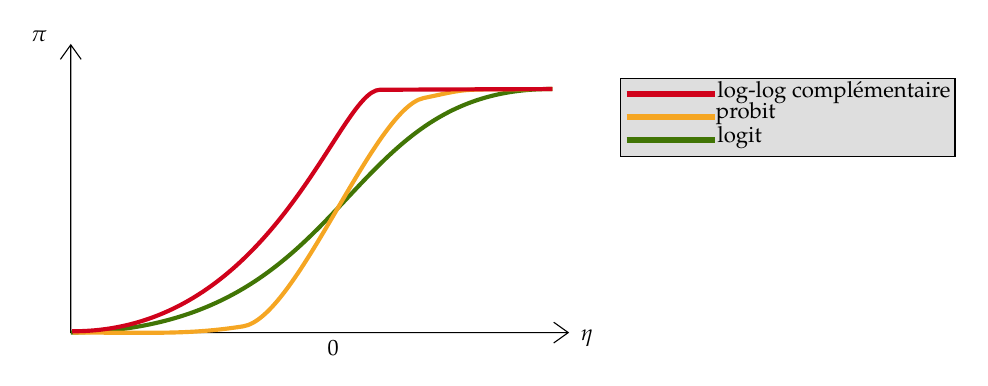
\begin{tikzpicture}[x=0.75pt,y=0.75pt,yscale=-1,xscale=1]
%uncomment if require: \path (0,300); %set diagram left start at 0, and has height of 300

%Shape: Axis 2D [id:dp48000806956401476] 
\draw  (98.17,148.64) -- (338.17,148.64)(98.5,10) -- (98.5,148.64) (331.17,143.64) -- (338.17,148.64) -- (331.17,153.64) (93.5,17) -- (98.5,10) -- (103.5,17)  ;
%Curve Lines [id:da6911332547105664] 
\draw [color={rgb, 255:red, 65; green, 117; blue, 5 }  ,draw opacity=1 ][line width=1.5]    (98.5,148.64) .. controls (236.5,146.64) and (225.5,30.64) .. (330.5,31.3) ;
%Curve Lines [id:da5236167901193742] 
\draw [color={rgb, 255:red, 245; green, 166; blue, 35 }  ,draw opacity=1 ][line width=1.5]    (99.5,148.64) .. controls (139.5,148.64) and (155.5,149.64) .. (181.5,145.64) .. controls (207.5,141.64) and (244.5,40.64) .. (268.5,35.64) .. controls (292.5,30.64) and (282.5,31.64) .. (330.5,31.3) ;
%Curve Lines [id:da7105130930164139] 
\draw [color={rgb, 255:red, 208; green, 2; blue, 27 }  ,draw opacity=1 ][line width=1.5]    (99.17,148) .. controls (196.5,148.3) and (227.5,31.64) .. (247.5,31.64) .. controls (267.5,31.64) and (231.5,31.64) .. (330.5,31.3) ;
%Shape: Rectangle [id:dp3994976422081038] 
\draw  [fill={rgb, 255:red, 222; green, 222; blue, 222 }  ,fill opacity=1 ] (363.54,26.08) -- (524.5,26.08) -- (524.5,63.64) -- (363.54,63.64) -- cycle ;
%Straight Lines [id:da8147114892565948] 
\draw [color={rgb, 255:red, 208; green, 2; blue, 27 }  ,draw opacity=1 ][line width=2.25]    (366.27,33.85) -- (408.99,33.85) ;
%Straight Lines [id:da8363691109245619] 
\draw [color={rgb, 255:red, 245; green, 166; blue, 35 }  ,draw opacity=1 ][line width=2.25]    (366.27,44.85) -- (408.99,44.85) ;
%Straight Lines [id:da07649571164976332] 
\draw [color={rgb, 255:red, 65; green, 117; blue, 5 }  ,draw opacity=1 ][line width=2.25]    (366.27,55.86) -- (408.99,55.86) ;

% Text Node
\draw (466.22,32.77) node  [font=\small] [align=left] {{\footnotesize log-log complémentaire}};
% Text Node
\draw (423.72,43.27) node  [font=\small] [align=left] {{\footnotesize probit}};
% Text Node
\draw (420.72,54.77) node  [font=\small] [align=left] {{\footnotesize logit}};
% Text Node
\draw (343,146) node [anchor=north west][inner sep=0.75pt]   [align=left] {{\footnotesize $\displaystyle \eta $}};
% Text Node
\draw (78,2) node [anchor=north west][inner sep=0.75pt]   [align=left] {{\footnotesize $\displaystyle \pi $}};
% Text Node
\draw (221,151) node [anchor=north west][inner sep=0.75pt]   [align=left] {{\footnotesize $\displaystyle 0$}};


\end{tikzpicture}

\end{center}

\paragraph{Note}	La cote, alias le \og \textit{odds ratio} \fg{}, est \lfbox[formula]{$\frac{\pi}{1	-	\pi}$}.


\subsection{Nominal}
On suppose qu'il y a $J$ catégories possibles pour la variable réponse. 
Pour modéliser avec la régression logistique, on :
\begin{enumerate}[label	=	\circled{\arabic*}{lightgray}]
	\item	Choisit une catégorie comme catégorie de base $1$.
	\item	Pour chacune des autres catégories, on trouve les cotes relatives (\og \textit{relative odds} \fg{}).
\end{enumerate}

Le logarithme de la cote de la catégorie $j$ relatif à la catégorie de base $1$ est :
\begin{align*}
	\ln \frac{\pi_{j}}{\pi_{1}}
	&=	\sum_{i	=	1}^{p} \beta_{ij} X_{i}
	=	\eta_{j}, \quad j	=	2, 3, \dots, J
\end{align*}

Alors, $\pi_{j}	=	\pi_{1}\textrm{e}^{\eta_{j}}$ et puisque les probabilités doivent sommer jusqu'à 1 :
\begin{align*}
	\pi_{1}
	&=	\frac{1}{1 + \sum_{k	=	2}^{J} \textrm{e}^{\eta_{k}}}	\\
	\pi_{j}
	&=	\frac{\textrm{e}^{\eta_{j}}}{1 + \sum_{k	=	2}^{J} \textrm{e}^{\eta_{k}}}, \quad j	=	2, 3, \dots, J
\end{align*}


\subsection{Ordinal}
\textbf{Modèle logit cumulatif}

\begin{align*}
	\frac{\Pr(Y \leq j)}{1	-	\Pr(Y \leq j)}
	&=	\frac{\sum_{k	=	1}^{j} \pi_{k}}{1	-	\sum_{k	=	1}^{j} \pi_{k}}	
	=	\frac{\pi_{1} + \hdots + \pi_{j}}{\pi_{j + 1} + \hdots + \pi_{J}}	\\
\end{align*}

Alors, avec les paramètres $\beta$ qui varient par catégorie $j$, :
\begin{align*}
	\ln\left(\frac{\pi_{1} + \hdots + \pi_{j}}{\pi_{j + 1} + \hdots + \pi_{J}}\right)
	&=	\sum_{i	=	1}^{p}\beta_{ij}X_{i}	\\
\end{align*}

\textbf{Modèle de cotes proportionnelles}	\\
Excepté l'intercepte, les paramètres $\beta$ ne varient pas par catégorie $j$ :
\begin{align*}
	\ln\left(\frac{\pi_{1} + \hdots + \pi_{j}}{\pi_{j + 1} + \hdots + \pi_{J}}\right)
	&=	\beta_{1j} + \sum_{i	=	2}^{p}\beta_{i}X_{i}	\\
\end{align*}

\textbf{Modèle logit de catégories adjacentes}
\begin{align*}
	\ln\left(\frac{\pi_{j}}{\pi_{j + 1}}\right)
	&=	\sum_{i	=	1}^{p}\beta_{ij}X_{i}	\\
\end{align*}

\textbf{Modèle logit de ratio continu}
\begin{align*}
	\frac{\Pr(Y	=	j)}{\Pr(Y	>	j)}
	&=	\frac{\pi_{j}}{\pi_{j + 1} + \hdots + \pi_{J}}
\end{align*}


\pagebreak
\section{Autres}
%	https://www.youtube.com/watch?v=0XfXHYDYoBA
\begin{tabular}{|	c	|	c	|}
Régression	&	Type de variable réponse	\\\hline
Linéaire		&	Continue	\\
Logistique	&	Binaire	\\
Poisson		&	Données de comptage	\\
Analyse de survie	&	Temps jusqu'à un événement	\\
\end{tabular}
\begin{itemize}
	\item	Logistique prédit la probabilité qu'un événement ait lieu.
	\item	Poisson prédit le \og \textit{rate} \fg{} auquel des événements aient lieu.
		\begin{itemize}
		\item	C'est-à-dire, le nombre de fois, ou la fréquence, d'un événement sur une période de temps.
		\item	Donc, le temps est fixé et on observe le nombre d'événements.
		\item	On ne peut pas simplement appliquer un modèle linéaire car les données suivent une distribution de Poisson, pas une distribution normale! 
		\item	Également, nous pouvons modéliser un \og \textit{offset} \fg{} pour considérer le temps d'exposition.
		\end{itemize}
	\item	Avec l'analyse de survie, on prédit le temps avant qu'un événement ait lieu.
		\begin{itemize}
		\item	Donc, le nombre d'événements est fixé à un et on veut savoir le temps avant qu'il ait lieu.
		\end{itemize}
\end{itemize}

\subsubsection{Poisson}
Il y a plusieurs façons de modéliser un même modèle de Poisson : 
\begin{enumerate}
	\item	Modéliser le taux comme une fonction log-linéaire des $x$ : $\lambda	=	\textrm{e}^{\beta_{0} + \beta_{1}x_{1} + \dots + \beta_{p}x_{p}}$.
		\begin{itemize}
		\item	Ceci puisque le taux $\lambda$ a une forme exponentielle.
		\end{itemize}
	\item	Modéliser le log du taux comme une fonction linéaire des $x$ : $\ln(\lambda)	=	\beta_{0} + \beta_{1}x_{1} + \dots + \beta_{p}x_{p}$.
		\begin{itemize}
		\item	Ceci permet de traiter le taux $\lambda$ avec un modèle linéaire.
		\item	L'avantage est la simplicité d'une ligne pour résumer le modèle.
		\item	Mathématiquement, les deux première équations sont équivalentes.
		\end{itemize}
	\item	Modéliser le log de la fréquence espérée avec un \og \textit{offset} \fg{} : $\ln(\text{E}[Y])	=	\ln(\text{E}[\lambda t])	=	\beta_{0} + \beta_{1}x_{1} + \dots + \beta_{p}x_{p}	+	\ln(t)$.
		\begin{itemize}
		\item	La deuxième équation représente ce que l'on fait en théorie alors que la troisième représente ce que l'on fait en pratique.
		\end{itemize}
\end{enumerate}

Hypothèses du modèle :
\begin{enumerate}
	\item	Les observations sont indépendantes.
		\begin{itemize}
		\item	Si, par exemple, avoir un récidive augmente la probabilité d'une deuxième récidive, alors le modèle n'est pas adéquat.
		\end{itemize}
	\item	Le taux auquel les événements se produisent est une fonction log-linéaire de $x$.
		\begin{itemize}
		\item	C'est-à-dire, le log du taux est une fonction linéaire des $x$.
		\end{itemize}
	\item	Les variations dans les $x$'s ont des effets multiplicatifs sur le nombre d'événements.
		\begin{itemize}
		\item	Par exemple, si on modélise la fréquence d'accidents auto alors on s'attend à ce que le nombre d'accidents sur deux ans soit le double du nombre d'accidents sur un an.
		\end{itemize}
	\item	La moyenne = variance = $\lambda$.
	\item	La taux est constant.
		\begin{itemize}
		\item	Donc, on pose que le taux est fixe.
		\item	Par exemple, la probabilité d'une récidive pourrait diminuer dans le temps.
		\end{itemize}
\end{enumerate}

Le modèle à deux gros problèmes, \underline{premièrement} la \textbf{sur-dispersion} où la variance est supérieure à la moyenne.
\begin{itemize}
		\item	C'est-à-dire que les données sont plus variables que ce qui est attendu.
		\item	Contrairement à la régression linéaire où l'estimation de la moyenne et du SSE sont séparées, l'estimation est la même pour le modèle de Poisson.
		\item	Il y a des multiples raisons pour lesquelles ceci peut arriver : 
			\begin{enumerate}
			\item	Nous n'avons pas inclus toutes les variables explicatives significatives dans le modèle.
			\item	La forme fonctionnelle du modèle est inadéquate (p. ex., les données ne sont pas log-linéaires).
			\item	Une variable est supposée d'être homogène alors qu'elle ne l'est pas.
				\begin{itemize}
				\item	P. ex., modéliser un groupe de fumeurs alors qu'il y a des sous-groupes (ceux qui font de l'exercice vs ceux qui n'en font pas, etc.)
				\end{itemize}
			\item	etc.
			\end{enumerate}
\end{itemize}

On peut calculer la \textbf{dispersion} et on désire qu'elle soit environ de 1.\\
Pour résoudre la sur-dispersion, on peut : 
\begin{enumerate}
	\item	On peut pondérer l'erreur type de tous les coefficients par la racine du paramètre de dispersion.
		\begin{itemize}
		\item	Ceci ne change pas les prévisions, plutôt ça augmente l'erreur type pour tenir compte du fait que la variabilité des données observées est plus élevée que ce à quoi on s'attendait.
		\end{itemize}
	\item	On peut ajuster un modèle avec une distribution binomiale négative.
		\begin{itemize}
		\item	Ceci permet d'estimer la fréquence et la variance séparément.
		\item	La variance sera plus grande, mais proportionnelle à la moyenne.
		\end{itemize}
\end{enumerate}


\underline{Deuxièmement}, \textbf{Données gonflées à zéro}. 
\begin{itemize}
	\item	L'idée est de modéliser la probabilité que l'événement ait lieu ou pas séparément de la fréquence.
	\item	On peut modéliser la probabilité avec un modèle logistique est la fréquence avec un modèle de Poisson.
\end{itemize}




\textbf{Matrice de confusion : }
\begin{center}


\tikzset{every picture/.style={line width=0.75pt}} %set default line width to 0.75pt        

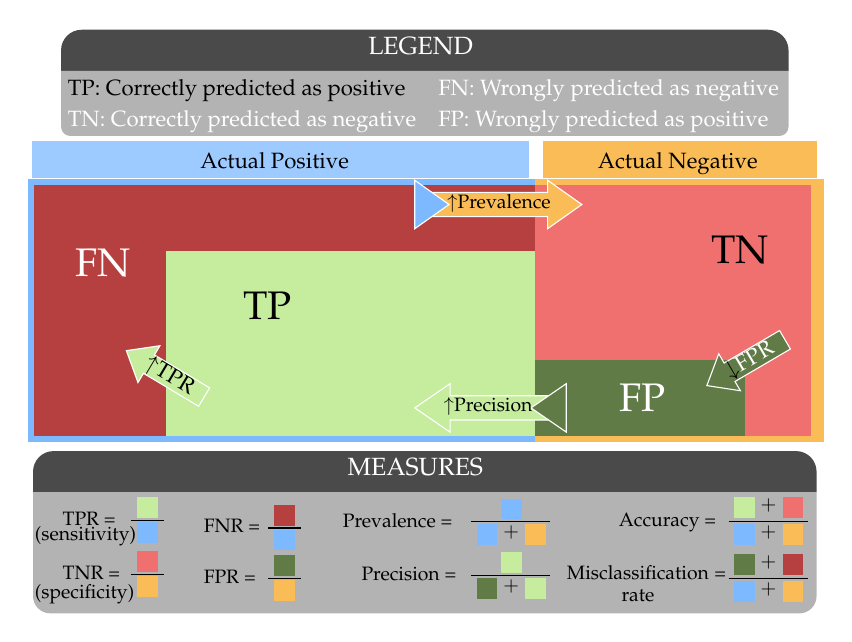
\begin{tikzpicture}[x=0.75pt,y=0.75pt,yscale=-1,xscale=1]
%uncomment if require: \path (0,366); %set diagram left start at 0, and has height of 366

%Rounded Same Side Corner Rect [id:dp5863189014777732] 
\draw  [draw opacity=0][fill={rgb, 255:red, 74; green, 74; blue, 74 }  ,fill opacity=1 ][line width=1.5]  (186.37,215.03) .. controls (186.37,209.57) and (190.8,205.14) .. (196.27,205.14) -- (553.98,205.14) .. controls (559.45,205.14) and (563.87,209.57) .. (563.87,215.03) -- (563.87,224.92) .. controls (563.87,224.92) and (563.87,224.92) .. (563.87,224.92) -- (186.37,224.92) .. controls (186.37,224.92) and (186.37,224.92) .. (186.37,224.92) -- cycle ;
%Rounded Same Side Corner Rect [id:dp10542736831068278] 
\draw  [draw opacity=0][fill={rgb, 255:red, 179; green, 179; blue, 179 }  ,fill opacity=1 ] (563.87,275.01) .. controls (563.87,279.61) and (560.15,283.33) .. (555.56,283.33) -- (194.69,283.33) .. controls (190.1,283.33) and (186.37,279.61) .. (186.37,275.01) -- (186.37,224.92) .. controls (186.37,224.92) and (186.37,224.92) .. (186.37,224.92) -- (563.87,224.92) .. controls (563.87,224.92) and (563.87,224.92) .. (563.87,224.92) -- cycle ;
%Flowchart: Process [id:dp2781782458228159] 
\draw  [draw opacity=0][fill={rgb, 255:red, 198; green, 237; blue, 158 }  ,fill opacity=1 ] (236.54,237.33) -- (246.54,237.33) -- (246.54,227.33) -- (236.54,227.33) -- cycle ;
%Flowchart: Process [id:dp6595006333689621] 
\draw  [draw opacity=0][fill={rgb, 255:red, 125; green, 185; blue, 255 }  ,fill opacity=1 ] (236.54,249.33) -- (246.54,249.33) -- (246.54,239.33) -- (236.54,239.33) -- cycle ;
%Straight Lines [id:da005645386209309766] 
\draw    (233.54,238.5) -- (249.54,238.5) ;

%Flowchart: Process [id:dp7524991543129134] 
\draw  [draw opacity=0][fill={rgb, 255:red, 125; green, 185; blue, 255 }  ,fill opacity=1 ] (302.54,253) -- (312.54,253) -- (312.54,243) -- (302.54,243) -- cycle ;
%Straight Lines [id:da5176971400521515] 
\draw    (299.54,242.17) -- (315.54,242.17) ;
%Flowchart: Process [id:dp9574550023533219] 
\draw  [draw opacity=0][fill={rgb, 255:red, 182; green, 64; blue, 64 }  ,fill opacity=1 ] (302.54,241) -- (312.54,241) -- (312.54,231) -- (302.54,231) -- cycle ;

%Flowchart: Process [id:dp6446573608226225] 
\draw  [draw opacity=0][fill={rgb, 255:red, 240; green, 111; blue, 111 }  ,fill opacity=1 ] (236.54,263.5) -- (246.54,263.5) -- (246.54,253.5) -- (236.54,253.5) -- cycle ;
%Flowchart: Process [id:dp6670926329350344] 
\draw  [draw opacity=0][fill={rgb, 255:red, 249; green, 188; blue, 87 }  ,fill opacity=1 ] (236.54,275.5) -- (246.54,275.5) -- (246.54,265.5) -- (236.54,265.5) -- cycle ;
%Straight Lines [id:da5832941059999399] 
\draw    (233.54,264.67) -- (249.54,264.67) ;

%Flowchart: Process [id:dp3885928458657999] 
\draw  [draw opacity=0][fill={rgb, 255:red, 249; green, 188; blue, 87 }  ,fill opacity=1 ] (302.54,277.33) -- (312.54,277.33) -- (312.54,267.33) -- (302.54,267.33) -- cycle ;
%Straight Lines [id:da3401710446338324] 
\draw    (299.54,266.5) -- (315.54,266.5) ;
%Flowchart: Process [id:dp6813365938208455] 
\draw  [draw opacity=0][fill={rgb, 255:red, 97; green, 123; blue, 71 }  ,fill opacity=1 ] (302.54,265.33) -- (312.54,265.33) -- (312.54,255.33) -- (302.54,255.33) -- cycle ;

%Flowchart: Process [id:dp26333217881412674] 
\draw  [draw opacity=0][fill={rgb, 255:red, 198; green, 237; blue, 158 }  ,fill opacity=1 ] (412.04,263.83) -- (422.04,263.83) -- (422.04,253.83) -- (412.04,253.83) -- cycle ;
%Flowchart: Process [id:dp33935301348671065] 
\draw  [draw opacity=0][fill={rgb, 255:red, 97; green, 123; blue, 71 }  ,fill opacity=1 ] (400.04,276.33) -- (410.04,276.33) -- (410.04,266.33) -- (400.04,266.33) -- cycle ;
%Straight Lines [id:da4578404875999813] 
\draw    (397.54,265) -- (435.54,265) ;
%Flowchart: Process [id:dp07704188689930547] 
\draw  [draw opacity=0][fill={rgb, 255:red, 198; green, 237; blue, 158 }  ,fill opacity=1 ] (423.54,276.33) -- (433.54,276.33) -- (433.54,266.33) -- (423.54,266.33) -- cycle ;

%Flowchart: Process [id:dp511192763925254] 
\draw  [draw opacity=0][fill={rgb, 255:red, 125; green, 185; blue, 255 }  ,fill opacity=1 ] (412.04,238) -- (422.04,238) -- (422.04,228) -- (412.04,228) -- cycle ;
%Flowchart: Process [id:dp8487027222224734] 
\draw  [draw opacity=0][fill={rgb, 255:red, 125; green, 185; blue, 255 }  ,fill opacity=1 ] (400.04,250.5) -- (410.04,250.5) -- (410.04,240.5) -- (400.04,240.5) -- cycle ;
%Straight Lines [id:da11748805900160852] 
\draw    (397.54,239.17) -- (435.54,239.17) ;
%Flowchart: Process [id:dp6757535243694623] 
\draw  [draw opacity=0][fill={rgb, 255:red, 249; green, 188; blue, 87 }  ,fill opacity=1 ] (423.54,250.5) -- (433.54,250.5) -- (433.54,240.5) -- (423.54,240.5) -- cycle ;

%Flowchart: Process [id:dp23257062904433523] 
\draw  [draw opacity=0][fill={rgb, 255:red, 125; green, 185; blue, 255 }  ,fill opacity=1 ] (524.04,250.5) -- (534.04,250.5) -- (534.04,240.5) -- (524.04,240.5) -- cycle ;
%Straight Lines [id:da16879793480007654] 
\draw    (521.54,239.17) -- (559.54,239.17) ;
%Flowchart: Process [id:dp629293047660624] 
\draw  [draw opacity=0][fill={rgb, 255:red, 249; green, 188; blue, 87 }  ,fill opacity=1 ] (547.54,250.5) -- (557.54,250.5) -- (557.54,240.5) -- (547.54,240.5) -- cycle ;
%Flowchart: Process [id:dp25903639593069716] 
\draw  [draw opacity=0][fill={rgb, 255:red, 198; green, 237; blue, 158 }  ,fill opacity=1 ] (524.04,237.5) -- (534.04,237.5) -- (534.04,227.5) -- (524.04,227.5) -- cycle ;
%Flowchart: Process [id:dp2784202862814029] 
\draw  [draw opacity=0][fill={rgb, 255:red, 240; green, 111; blue, 111 }  ,fill opacity=1 ] (547.54,237.5) -- (557.54,237.5) -- (557.54,227.5) -- (547.54,227.5) -- cycle ;

%Flowchart: Process [id:dp5706215732887201] 
\draw  [draw opacity=0][fill={rgb, 255:red, 125; green, 185; blue, 255 }  ,fill opacity=1 ] (524.04,277.83) -- (534.04,277.83) -- (534.04,267.83) -- (524.04,267.83) -- cycle ;
%Straight Lines [id:da24052635124853383] 
\draw    (521.54,266.5) -- (559.54,266.5) ;
%Flowchart: Process [id:dp8806206355646873] 
\draw  [draw opacity=0][fill={rgb, 255:red, 249; green, 188; blue, 87 }  ,fill opacity=1 ] (547.54,277.83) -- (557.54,277.83) -- (557.54,267.83) -- (547.54,267.83) -- cycle ;
%Flowchart: Process [id:dp025661689438194246] 
\draw  [draw opacity=0][fill={rgb, 255:red, 97; green, 123; blue, 71 }  ,fill opacity=1 ] (524.04,264.83) -- (534.04,264.83) -- (534.04,254.83) -- (524.04,254.83) -- cycle ;
%Flowchart: Process [id:dp07416724651822326] 
\draw  [draw opacity=0][fill={rgb, 255:red, 182; green, 64; blue, 64 }  ,fill opacity=1 ] (547.54,264.83) -- (557.54,264.83) -- (557.54,254.83) -- (547.54,254.83) -- cycle ;


%Shape: Rectangle [id:dp9078887636984747] 
\draw  [color={rgb, 255:red, 125; green, 185; blue, 255 }  ,draw opacity=1 ][fill={rgb, 255:red, 125; green, 185; blue, 255 }  ,fill opacity=1 ][line width=4.5]  (186.79,76.98) -- (428.29,76.98) -- (428.29,198) -- (186.79,198) -- cycle ;
%Shape: Rectangle [id:dp6719473196737591] 
\draw  [color={rgb, 255:red, 249; green, 188; blue, 87 }  ,draw opacity=1 ][fill={rgb, 255:red, 249; green, 188; blue, 87 }  ,fill opacity=1 ][line width=4.5]  (431.29,76.98) -- (564.29,76.98) -- (564.29,198) -- (431.29,198) -- cycle ;
%Shape: Rectangle [id:dp8554811027992568] 
\draw  [draw opacity=0][fill={rgb, 255:red, 240; green, 111; blue, 111 }  ,fill opacity=1 ][line width=0.75]  (427.96,76.98) -- (560.96,76.98) -- (560.96,198) -- (427.96,198) -- cycle ;
%Shape: Rectangle [id:dp4666790964474916] 
\draw  [draw opacity=0][fill={rgb, 255:red, 182; green, 64; blue, 64 }  ,fill opacity=1 ] (186.79,76.98) -- (428.29,76.98) -- (428.29,198) -- (186.79,198) -- cycle ;
%Shape: Rectangle [id:dp4684932062372884] 
\draw  [draw opacity=0][fill={rgb, 255:red, 125; green, 185; blue, 255 }  ,fill opacity=0.75 ] (185.96,55.67) -- (425.29,55.67) -- (425.29,73.33) -- (185.96,73.33) -- cycle ;
%Shape: Rectangle [id:dp7538608016518991] 
\draw  [draw opacity=0][fill={rgb, 255:red, 249; green, 188; blue, 87 }  ,fill opacity=1 ] (432.29,55.67) -- (563.96,55.67) -- (563.96,73.33) -- (432.29,73.33) -- cycle ;
%Shape: Rectangle [id:dp575388567694743] 
\draw  [draw opacity=0][fill={rgb, 255:red, 198; green, 237; blue, 158 }  ,fill opacity=1 ] (250.29,108.8) -- (428.29,108.8) -- (428.29,198) -- (250.29,198) -- cycle ;
%Shape: Rectangle [id:dp694025502587706] 
\draw  [draw opacity=0][fill={rgb, 255:red, 97; green, 123; blue, 71 }  ,fill opacity=1 ] (428.29,161.33) -- (529.29,161.33) -- (529.29,198) -- (428.29,198) -- cycle ;
%Left Arrow [id:dp159442790435544] 
\draw  [color={rgb, 255:red, 255; green, 255; blue, 255 }  ,draw opacity=1 ][fill={rgb, 255:red, 97; green, 123; blue, 71 }  ,fill opacity=1 ] (511.02,173.58) -- (516.74,158.26) -- (519.35,162.71) -- (546.06,147.06) -- (551.28,155.96) -- (524.57,171.61) -- (527.18,176.07) -- cycle ;

%Left Arrow [id:dp2567253964557259] 
\draw  [color={rgb, 255:red, 255; green, 255; blue, 255 }  ,draw opacity=1 ][fill={rgb, 255:red, 198; green, 237; blue, 158 }  ,fill opacity=1 ] (231.33,156.74) -- (247.51,154.38) -- (244.87,158.81) -- (271.45,174.68) -- (266.16,183.54) -- (239.58,167.67) -- (236.93,172.1) -- cycle ;

%Left Arrow [id:dp4712888920317464] 
\draw  [color={rgb, 255:red, 255; green, 255; blue, 255 }  ,draw opacity=1 ][fill={rgb, 255:red, 198; green, 237; blue, 158 }  ,fill opacity=1 ] (370.29,184.33) -- (387.29,172.66) -- (387.29,178.5) -- (440.29,178.5) -- (440.29,190.17) -- (387.29,190.17) -- (387.29,196) -- cycle ;
%Left Arrow [id:dp3521145387427629] 
\draw  [color={rgb, 255:red, 255; green, 255; blue, 255 }  ,draw opacity=1 ][fill={rgb, 255:red, 97; green, 123; blue, 71 }  ,fill opacity=1 ] (426.29,184.33) -- (443.29,172.66) -- (443.29,178.5) -- (443.29,178.5) -- (443.29,190.17) -- (443.29,190.17) -- (443.29,196) -- cycle ;

%Left Arrow [id:dp8166384807624658] 
\draw  [color={rgb, 255:red, 255; green, 255; blue, 255 }  ,draw opacity=1 ][fill={rgb, 255:red, 249; green, 188; blue, 87 }  ,fill opacity=1 ] (450.8,86.33) -- (434.29,74.66) -- (434.29,80.5) -- (370.29,80.5) -- (370.29,92.17) -- (434.29,92.17) -- (434.29,98) -- cycle ;
%Left Arrow [id:dp8194414952038565] 
\draw  [color={rgb, 255:red, 255; green, 255; blue, 255 }  ,draw opacity=1 ][fill={rgb, 255:red, 125; green, 185; blue, 255 }  ,fill opacity=1 ] (386.8,86.33) -- (370.29,74.66) -- (370.29,80.5) -- (370.29,80.5) -- (370.29,92.17) -- (370.29,92.17) -- (370.29,98) -- cycle ;


%Rounded Same Side Corner Rect [id:dp01839882980964913] 
\draw  [draw opacity=0][fill={rgb, 255:red, 74; green, 74; blue, 74 }  ,fill opacity=1 ][line width=1.5]  (199.87,12.03) .. controls (199.87,6.57) and (204.3,2.14) .. (209.77,2.14) -- (540.48,2.14) .. controls (545.95,2.14) and (550.37,6.57) .. (550.37,12.03) -- (550.37,21.92) .. controls (550.37,21.92) and (550.37,21.92) .. (550.37,21.92) -- (199.87,21.92) .. controls (199.87,21.92) and (199.87,21.92) .. (199.87,21.92) -- cycle ;
%Rounded Same Side Corner Rect [id:dp42232070994654003] 
\draw  [draw opacity=0][fill={rgb, 255:red, 179; green, 179; blue, 179 }  ,fill opacity=1 ] (550.37,48.86) .. controls (550.37,51.33) and (548.37,53.33) .. (545.9,53.33) -- (204.35,53.33) .. controls (201.88,53.33) and (199.87,51.33) .. (199.87,48.86) -- (199.87,21.92) .. controls (199.87,21.92) and (199.87,21.92) .. (199.87,21.92) -- (550.37,21.92) .. controls (550.37,21.92) and (550.37,21.92) .. (550.37,21.92) -- cycle ;


% Text Node
\draw (267.37,236.67) node [anchor=north west][inner sep=0.75pt]  [font=\scriptsize] [align=left] {FNR = };
% Text Node
\draw (267.37,261) node [anchor=north west][inner sep=0.75pt]  [font=\scriptsize] [align=left] {FPR = };
% Text Node
\draw (343.37,259.5) node [anchor=north west][inner sep=0.75pt]  [font=\scriptsize] [align=left] {Precision = };
% Text Node
\draw (411.54,265.83) node [anchor=north west][inner sep=0.75pt]  [font=\scriptsize] [align=left] {$\displaystyle +$};
% Text Node
\draw (535.54,267.33) node [anchor=north west][inner sep=0.75pt]  [font=\scriptsize] [align=left] {$\displaystyle +$};
% Text Node
\draw (440.37,259) node [anchor=north west][inner sep=0.75pt]  [font=\scriptsize] [align=left] {\begin{minipage}[lt]{54.30085600000001pt}\setlength\topsep{0pt}
\begin{center}
Misclassification\\rate 
\end{center}

\end{minipage}};
% Text Node
\draw (535.54,254.33) node [anchor=north west][inner sep=0.75pt]  [font=\scriptsize] [align=left] {$\displaystyle +$};
% Text Node
\draw (513.37,262) node [anchor=north west][inner sep=0.75pt]  [font=\scriptsize] [align=left] {= };
% Text Node
\draw (535.54,240) node [anchor=north west][inner sep=0.75pt]  [font=\scriptsize] [align=left] {$\displaystyle +$};
% Text Node
\draw (467.37,233.67) node [anchor=north west][inner sep=0.75pt]  [font=\scriptsize] [align=left] {Accuracy = };
% Text Node
\draw (535.54,227) node [anchor=north west][inner sep=0.75pt]  [font=\scriptsize] [align=left] {$\displaystyle +$};
% Text Node
\draw (334.37,233.67) node [anchor=north west][inner sep=0.75pt]  [font=\scriptsize] [align=left] {Prevalence = };
% Text Node
\draw (411.54,240) node [anchor=north west][inner sep=0.75pt]  [font=\scriptsize] [align=left] {$\displaystyle +$};
% Text Node
\draw (243.09,156.56) node [anchor=north west][inner sep=0.75pt]  [font=\scriptsize,rotate=-30.84] [align=left] {{\footnotesize $\displaystyle \uparrow $TPR}};
% Text Node
\draw (516.52,163.19) node [anchor=north west][inner sep=0.75pt]  [font=\scriptsize,rotate=-329.62] [align=left] {{\footnotesize $\displaystyle \downarrow $\textcolor[rgb]{1,1,1}{FPR}}};
% Text Node
\draw (382.95,178.25) node [anchor=north west][inner sep=0.75pt]  [font=\scriptsize] [align=left] {{\scriptsize $\displaystyle \uparrow $Precision}};
% Text Node
\draw (384.63,80.25) node [anchor=north west][inner sep=0.75pt]  [font=\scriptsize] [align=left] {{\scriptsize $\displaystyle \uparrow $Prevalence}};
% Text Node
\draw (199.37,233) node [anchor=north west][inner sep=0.75pt]  [font=\scriptsize] [align=left] {TPR = };
% Text Node
\draw (186,240) node [anchor=north west][inner sep=0.75pt]  [font=\scriptsize] [align=left] {{\scriptsize (sensitivity)}};
% Text Node
\draw (199.37,259.17) node [anchor=north west][inner sep=0.75pt]  [font=\scriptsize] [align=left] {TNR = };
% Text Node
\draw (186,268.17) node [anchor=north west][inner sep=0.75pt]  [font=\scriptsize] [align=left] {{\scriptsize (specificity)}};
% Text Node
\draw (264.04,60.17) node [anchor=north west][inner sep=0.75pt]  [font=\footnotesize,color={rgb, 255:red, 0; green, 0; blue, 0 }  ,opacity=1 ] [align=left] {\begin{minipage}[lt]{56.241644pt}\setlength\topsep{0pt}
\begin{center}
Actual Positive
\end{center}

\end{minipage}};
% Text Node
\draw (455.79,60.17) node [anchor=north west][inner sep=0.75pt]  [font=\footnotesize,color={rgb, 255:red, 0; green, 0; blue, 0 }  ,opacity=1 ] [align=left] {\begin{minipage}[lt]{59.875428pt}\setlength\topsep{0pt}
\begin{center}
Actual Negative
\end{center}

\end{minipage}};
% Text Node
\draw (464.29,171.17) node [anchor=north west][inner sep=0.75pt]  [font=\Large,color={rgb, 255:red, 255; green, 255; blue, 255 }  ,opacity=1 ] [align=left] {\begin{minipage}[lt]{21.490856pt}\setlength\topsep{0pt}
\begin{center}\textcolor{white}{
FP}
\end{center}

\end{minipage}};
% Text Node
\draw (204.04,106.17) node [anchor=north west][inner sep=0.75pt]  [font=\Large,color={rgb, 255:red, 255; green, 255; blue, 255 }  ,opacity=1 ] [align=left] {\begin{minipage}[lt]{22.305428000000003pt}\setlength\topsep{0pt}
\begin{center}\textcolor{white}{
FN}
\end{center}

\end{minipage}};
% Text Node
\draw (510.96,99.99) node [anchor=north west][inner sep=0.75pt]  [font=\Large,color={rgb, 255:red, 0; green, 0; blue, 0 }  ,opacity=1 ] [align=left] {\begin{minipage}[lt]{22.305428000000003pt}\setlength\topsep{0pt}
\begin{center}
TN
\end{center}

\end{minipage}};
% Text Node
\draw (283.79,126.9) node [anchor=north west][inner sep=0.75pt]  [font=\Large,color={rgb, 255:red, 0; green, 0; blue, 0 }  ,opacity=1 ] [align=left] {\begin{minipage}[lt]{21.490856pt}\setlength\topsep{0pt}
\begin{center}
TP
\end{center}

\end{minipage}};
% Text Node
\draw (336.62,207.19) node [anchor=north west][inner sep=0.75pt]  [font=\small,color={rgb, 255:red, 255; green, 255; blue, 255 }  ,opacity=1 ] [align=left] {MEASURES};
% Text Node
\draw (346.62,4.53) node [anchor=north west][inner sep=0.75pt]  [font=\small,color={rgb, 255:red, 255; green, 255; blue, 255 }  ,opacity=1 ] [align=left] {LEGEND};
% Text Node
\draw (201.87,24.92) node [anchor=north west][inner sep=0.75pt]  [font=\small,color={rgb, 255:red, 255; green, 255; blue, 255 }  ,opacity=1 ] [align=left] {{\footnotesize \textcolor[rgb]{0,0,0}{TP: Correctly predicted as positive}}\\{\footnotesize TN: Correctly predicted as negative}};
% Text Node
\draw (380.37,24.92) node [anchor=north west][inner sep=0.75pt]  [font=\small,color={rgb, 255:red, 255; green, 255; blue, 255 }  ,opacity=1 ] [align=left] {{\footnotesize FN: Wrongly predicted as negative}\\{\footnotesize FP: Wrongly predicted as positive}};


\end{tikzpicture}
\end{center}


\section{Erreur}

\begin{description}
	\item[Écart-type]	Mesure la variation \underline{entre les observations} d'\textbf{un} ensemble de données.
		\begin{itemize}[leftmargin = *]
		\item	\og \textit{standard deviation} \fg{}.
		\end{itemize}
		\begin{center}

\tikzset{every picture/.style={line width=0.75pt}} %set default line width to 0.75pt        

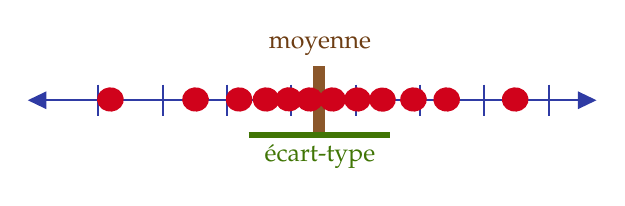
\begin{tikzpicture}[x=0.75pt,y=0.75pt,yscale=-1,xscale=1]
%uncomment if require: \path (0,174); %set diagram left start at 0, and has height of 174

%Straight Lines [id:da5554502737558269] 
\draw [color={rgb, 255:red, 47; green, 59; blue, 164 }  ,draw opacity=1 ][line width=0.75]    (279.83,38) -- (547.83,38) (310.83,30.5) -- (310.83,45.5)(341.83,30.5) -- (341.83,45.5)(372.83,30.5) -- (372.83,45.5)(403.83,30.5) -- (403.83,45.5)(434.83,30.5) -- (434.83,45.5)(465.83,30.5) -- (465.83,45.5)(496.83,30.5) -- (496.83,45.5)(527.83,30.5) -- (527.83,45.5) ;
\draw [shift={(550.83,38)}, rotate = 180] [fill={rgb, 255:red, 47; green, 59; blue, 164 }  ,fill opacity=1 ][line width=0.08]  [draw opacity=0] (8.93,-4.29) -- (0,0) -- (8.93,4.29) -- cycle    ;
\draw [shift={(276.83,38)}, rotate = 0] [fill={rgb, 255:red, 47; green, 59; blue, 164 }  ,fill opacity=1 ][line width=0.08]  [draw opacity=0] (8.93,-4.29) -- (0,0) -- (8.93,4.29) -- cycle    ;
%Straight Lines [id:da6666232383065853] 
\draw [color={rgb, 255:red, 139; green, 87; blue, 42 }  ,draw opacity=1 ][line width=2.25]    (415.67,54.92) -- (415.67,21.42)(418.67,54.92) -- (418.67,21.42) ;
%Flowchart: Connector [id:dp30389051575543746] 
\draw  [draw opacity=0][fill={rgb, 255:red, 208; green, 2; blue, 27 }  ,fill opacity=1 ] (320.71,33.09) .. controls (317.96,31.04) and (313.9,31.42) .. (311.65,33.93) .. controls (309.4,36.44) and (309.81,40.13) .. (312.57,42.17) .. controls (315.33,44.21) and (319.39,43.84) .. (321.63,41.33) .. controls (323.88,38.82) and (323.47,35.13) .. (320.71,33.09) -- cycle ;
%Flowchart: Connector [id:dp8054636909486927] 
\draw  [draw opacity=0][fill={rgb, 255:red, 208; green, 2; blue, 27 }  ,fill opacity=1 ] (382.71,33.09) .. controls (379.96,31.04) and (375.9,31.42) .. (373.65,33.93) .. controls (371.4,36.44) and (371.81,40.13) .. (374.57,42.17) .. controls (377.33,44.21) and (381.39,43.84) .. (383.63,41.33) .. controls (385.88,38.82) and (385.47,35.13) .. (382.71,33.09) -- cycle ;
%Flowchart: Connector [id:dp4481822183684774] 
\draw  [draw opacity=0][fill={rgb, 255:red, 208; green, 2; blue, 27 }  ,fill opacity=1 ] (361.71,33.09) .. controls (358.96,31.04) and (354.9,31.42) .. (352.65,33.93) .. controls (350.4,36.44) and (350.81,40.13) .. (353.57,42.17) .. controls (356.33,44.21) and (360.39,43.84) .. (362.63,41.33) .. controls (364.88,38.82) and (364.47,35.13) .. (361.71,33.09) -- cycle ;
%Flowchart: Connector [id:dp9320426369464008] 
\draw  [draw opacity=0][fill={rgb, 255:red, 208; green, 2; blue, 27 }  ,fill opacity=1 ] (416.71,33.09) .. controls (413.96,31.04) and (409.9,31.42) .. (407.65,33.93) .. controls (405.4,36.44) and (405.81,40.13) .. (408.57,42.17) .. controls (411.33,44.21) and (415.39,43.84) .. (417.63,41.33) .. controls (419.88,38.82) and (419.47,35.13) .. (416.71,33.09) -- cycle ;
%Flowchart: Connector [id:dp5645916521008547] 
\draw  [draw opacity=0][fill={rgb, 255:red, 208; green, 2; blue, 27 }  ,fill opacity=1 ] (395.71,33.09) .. controls (392.96,31.04) and (388.9,31.42) .. (386.65,33.93) .. controls (384.4,36.44) and (384.81,40.13) .. (387.57,42.17) .. controls (390.33,44.21) and (394.39,43.84) .. (396.63,41.33) .. controls (398.88,38.82) and (398.47,35.13) .. (395.71,33.09) -- cycle ;
%Flowchart: Connector [id:dp9615392127090878] 
\draw  [draw opacity=0][fill={rgb, 255:red, 208; green, 2; blue, 27 }  ,fill opacity=1 ] (439.71,33.09) .. controls (436.96,31.04) and (432.9,31.42) .. (430.65,33.93) .. controls (428.4,36.44) and (428.81,40.13) .. (431.57,42.17) .. controls (434.33,44.21) and (438.39,43.84) .. (440.63,41.33) .. controls (442.88,38.82) and (442.47,35.13) .. (439.71,33.09) -- cycle ;
%Flowchart: Connector [id:dp18343654664200626] 
\draw  [draw opacity=0][fill={rgb, 255:red, 208; green, 2; blue, 27 }  ,fill opacity=1 ] (427.71,33.09) .. controls (424.96,31.04) and (420.9,31.42) .. (418.65,33.93) .. controls (416.4,36.44) and (416.81,40.13) .. (419.57,42.17) .. controls (422.33,44.21) and (426.39,43.84) .. (428.63,41.33) .. controls (430.88,38.82) and (430.47,35.13) .. (427.71,33.09) -- cycle ;
%Flowchart: Connector [id:dp49357374316679636] 
\draw  [draw opacity=0][fill={rgb, 255:red, 208; green, 2; blue, 27 }  ,fill opacity=1 ] (466.71,33.09) .. controls (463.96,31.04) and (459.9,31.42) .. (457.65,33.93) .. controls (455.4,36.44) and (455.81,40.13) .. (458.57,42.17) .. controls (461.33,44.21) and (465.39,43.84) .. (467.63,41.33) .. controls (469.88,38.82) and (469.47,35.13) .. (466.71,33.09) -- cycle ;
%Flowchart: Connector [id:dp5732145021055151] 
\draw  [draw opacity=0][fill={rgb, 255:red, 208; green, 2; blue, 27 }  ,fill opacity=1 ] (451.78,33.16) .. controls (449.02,31.12) and (444.96,31.49) .. (442.71,34) .. controls (440.46,36.51) and (440.88,40.2) .. (443.63,42.24) .. controls (446.39,44.28) and (450.45,43.91) .. (452.7,41.4) .. controls (454.94,38.89) and (454.53,35.2) .. (451.78,33.16) -- cycle ;
%Flowchart: Connector [id:dp9989913792112952] 
\draw  [draw opacity=0][fill={rgb, 255:red, 208; green, 2; blue, 27 }  ,fill opacity=1 ] (515.71,33.09) .. controls (512.96,31.04) and (508.9,31.42) .. (506.65,33.93) .. controls (504.4,36.44) and (504.81,40.13) .. (507.57,42.17) .. controls (510.33,44.21) and (514.39,43.84) .. (516.63,41.33) .. controls (518.88,38.82) and (518.47,35.13) .. (515.71,33.09) -- cycle ;
%Flowchart: Connector [id:dp2709053942707078] 
\draw  [draw opacity=0][fill={rgb, 255:red, 208; green, 2; blue, 27 }  ,fill opacity=1 ] (482.71,33.09) .. controls (479.96,31.04) and (475.9,31.42) .. (473.65,33.93) .. controls (471.4,36.44) and (471.81,40.13) .. (474.57,42.17) .. controls (477.33,44.21) and (481.39,43.84) .. (483.63,41.33) .. controls (485.88,38.82) and (485.47,35.13) .. (482.71,33.09) -- cycle ;
%Flowchart: Connector [id:dp7446426173106822] 
\draw  [draw opacity=0][fill={rgb, 255:red, 208; green, 2; blue, 27 }  ,fill opacity=1 ] (406.65,33.02) .. controls (403.89,30.97) and (399.84,31.35) .. (397.59,33.86) .. controls (395.34,36.36) and (395.75,40.05) .. (398.51,42.1) .. controls (401.27,44.14) and (405.32,43.77) .. (407.57,41.26) .. controls (409.82,38.75) and (409.41,35.06) .. (406.65,33.02) -- cycle ;
%Straight Lines [id:da9789557877821047] 
\draw [color={rgb, 255:red, 65; green, 117; blue, 5 }  ,draw opacity=1 ][line width=2.25]    (383.17,54.92) -- (451.17,54.92) ;

% Text Node
\draw (417.58,12) node  [color={rgb, 255:red, 109; green, 61; blue, 19 }  ,opacity=1 ] [align=left] {{\small moyenne}};
% Text Node
\draw (417.58,65) node  [font=\small,color={rgb, 255:red, 109; green, 61; blue, 19 }  ,opacity=1 ] [align=left] {{\small \textcolor[rgb]{0.25,0.46,0.02}{écart-type}}};


\end{tikzpicture}
		\end{center}
	\item[Erreur type]	Mesure la variation \underline{entre les moyennes} de \textbf{plusieurs} ensembles de données.
		\begin{itemize}[leftmargin = *]
		\item	\og \textit{standard error} \fg{}.
		\end{itemize}
		\begin{center}
		

\tikzset{every picture/.style={line width=0.75pt}} %set default line width to 0.75pt        

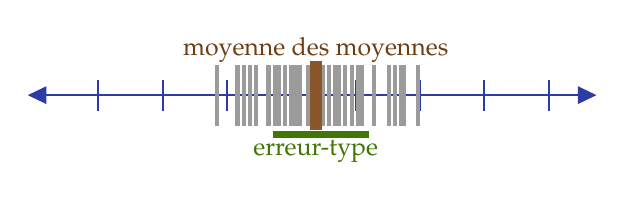
\begin{tikzpicture}[x=0.75pt,y=0.75pt,yscale=-1,xscale=1]
%uncomment if require: \path (0,174); %set diagram left start at 0, and has height of 174

%Straight Lines [id:da8220125436751056] 
\draw [color={rgb, 255:red, 47; green, 59; blue, 164 }  ,draw opacity=1 ][line width=0.75]    (281.83,118) -- (549.83,118) (312.83,110.5) -- (312.83,125.5)(343.83,110.5) -- (343.83,125.5)(374.83,110.5) -- (374.83,125.5)(405.83,110.5) -- (405.83,125.5)(436.83,110.5) -- (436.83,125.5)(467.83,110.5) -- (467.83,125.5)(498.83,110.5) -- (498.83,125.5)(529.83,110.5) -- (529.83,125.5) ;
\draw [shift={(552.83,118)}, rotate = 180] [fill={rgb, 255:red, 47; green, 59; blue, 164 }  ,fill opacity=1 ][line width=0.08]  [draw opacity=0] (8.93,-4.29) -- (0,0) -- (8.93,4.29) -- cycle    ;
\draw [shift={(278.83,118)}, rotate = 0] [fill={rgb, 255:red, 47; green, 59; blue, 164 }  ,fill opacity=1 ][line width=0.08]  [draw opacity=0] (8.93,-4.29) -- (0,0) -- (8.93,4.29) -- cycle    ;
%Straight Lines [id:da052261111869088106] 
\draw [color={rgb, 255:red, 155; green, 155; blue, 155 }  ,draw opacity=1 ][line width=1.5]    (415.83,132.67) -- (415.83,103.33) ;
%Straight Lines [id:da25533101510311673] 
\draw [color={rgb, 255:red, 155; green, 155; blue, 155 }  ,draw opacity=1 ][line width=1.5]    (420.83,132.67) -- (420.83,103.33) ;
%Straight Lines [id:da6426635244738363] 
\draw [color={rgb, 255:red, 155; green, 155; blue, 155 }  ,draw opacity=1 ][line width=1.5]    (426.83,132.67) -- (426.83,103.33) ;
%Straight Lines [id:da6924171841728055] 
\draw [color={rgb, 255:red, 155; green, 155; blue, 155 }  ,draw opacity=1 ][line width=1.5]    (423.83,132.67) -- (423.83,103.33) ;
%Straight Lines [id:da19673873838231448] 
\draw [color={rgb, 255:red, 155; green, 155; blue, 155 }  ,draw opacity=1 ][line width=1.5]    (428.83,132.67) -- (428.83,103.33) ;
%Straight Lines [id:da9733057591182157] 
\draw [color={rgb, 255:red, 155; green, 155; blue, 155 }  ,draw opacity=1 ][line width=1.5]    (434.83,132.67) -- (434.83,103.33) ;
%Straight Lines [id:da23648190125390167] 
\draw [color={rgb, 255:red, 155; green, 155; blue, 155 }  ,draw opacity=1 ][line width=1.5]    (394.83,132.67) -- (394.83,103.33) ;
%Straight Lines [id:da1303046815942539] 
\draw [color={rgb, 255:red, 155; green, 155; blue, 155 }  ,draw opacity=1 ][line width=1.5]    (399.83,132.67) -- (399.83,103.33) ;
%Straight Lines [id:da6128601437483194] 
\draw [color={rgb, 255:red, 155; green, 155; blue, 155 }  ,draw opacity=1 ][line width=1.5]    (405.83,132.67) -- (405.83,103.33) ;
%Straight Lines [id:da36533401916878416] 
\draw [color={rgb, 255:red, 155; green, 155; blue, 155 }  ,draw opacity=1 ][line width=1.5]    (402.83,132.67) -- (402.83,103.33) ;
%Straight Lines [id:da0761803178503282] 
\draw [color={rgb, 255:red, 155; green, 155; blue, 155 }  ,draw opacity=1 ][line width=1.5]    (407.83,132.67) -- (407.83,103.33) ;
%Straight Lines [id:da4536124738403875] 
\draw [color={rgb, 255:red, 155; green, 155; blue, 155 }  ,draw opacity=1 ][line width=1.5]    (413.83,132.67) -- (413.83,103.33) ;
%Straight Lines [id:da2518902010718611] 
\draw [color={rgb, 255:red, 155; green, 155; blue, 155 }  ,draw opacity=1 ][line width=1.5]    (459.83,132.67) -- (459.83,103.33) ;
%Straight Lines [id:da6762200116514319] 
\draw [color={rgb, 255:red, 155; green, 155; blue, 155 }  ,draw opacity=1 ][line width=1.5]    (452.83,132.67) -- (452.83,103.33) ;
%Straight Lines [id:da023011435062046726] 
\draw [color={rgb, 255:red, 155; green, 155; blue, 155 }  ,draw opacity=1 ][line width=1.5]    (452.83,132.67) -- (452.83,103.33) ;
%Straight Lines [id:da5498951842262785] 
\draw [color={rgb, 255:red, 155; green, 155; blue, 155 }  ,draw opacity=1 ][line width=1.5]    (458.83,132.67) -- (458.83,103.33) ;
%Straight Lines [id:da8590490011467546] 
\draw [color={rgb, 255:red, 155; green, 155; blue, 155 }  ,draw opacity=1 ][line width=1.5]    (455.83,132.67) -- (455.83,103.33) ;
%Straight Lines [id:da8877231722848657] 
\draw [color={rgb, 255:red, 155; green, 155; blue, 155 }  ,draw opacity=1 ][line width=1.5]    (466.83,132.67) -- (466.83,103.33) ;
%Straight Lines [id:da05542853037330375] 
\draw [color={rgb, 255:red, 155; green, 155; blue, 155 }  ,draw opacity=1 ][line width=1.5]    (426.83,132.67) -- (426.83,103.33) ;
%Straight Lines [id:da12451183170415692] 
\draw [color={rgb, 255:red, 155; green, 155; blue, 155 }  ,draw opacity=1 ][line width=1.5]    (431.83,132.67) -- (431.83,103.33) ;
%Straight Lines [id:da512024470962503] 
\draw [color={rgb, 255:red, 155; green, 155; blue, 155 }  ,draw opacity=1 ][line width=1.5]    (437.83,132.67) -- (437.83,103.33) ;
%Straight Lines [id:da026634526507703926] 
\draw [color={rgb, 255:red, 155; green, 155; blue, 155 }  ,draw opacity=1 ][line width=1.5]    (434.83,132.67) -- (434.83,103.33) ;
%Straight Lines [id:da04652506773140819] 
\draw [color={rgb, 255:red, 155; green, 155; blue, 155 }  ,draw opacity=1 ][line width=1.5]    (439.83,132.67) -- (439.83,103.33) ;
%Straight Lines [id:da7028504306628334] 
\draw [color={rgb, 255:red, 155; green, 155; blue, 155 }  ,draw opacity=1 ][line width=1.5]    (445.83,132.67) -- (445.83,103.33) ;
%Straight Lines [id:da3097660501000492] 
\draw [color={rgb, 255:red, 155; green, 155; blue, 155 }  ,draw opacity=1 ][line width=1.5]    (410.17,132.67) -- (410.17,103.33) ;
%Straight Lines [id:da6597565804975323] 
\draw [color={rgb, 255:red, 155; green, 155; blue, 155 }  ,draw opacity=1 ][line width=1.5]    (416.83,132.67) -- (416.83,103.33) ;
%Straight Lines [id:da9737145894752222] 
\draw [color={rgb, 255:red, 155; green, 155; blue, 155 }  ,draw opacity=1 ][line width=1.5]    (416.83,132.67) -- (416.83,103.33) ;
%Straight Lines [id:da6435581383162627] 
\draw [color={rgb, 255:red, 155; green, 155; blue, 155 }  ,draw opacity=1 ][line width=1.5]    (369.83,132.67) -- (369.83,103.33) ;
%Straight Lines [id:da02223066622835468] 
\draw [color={rgb, 255:red, 155; green, 155; blue, 155 }  ,draw opacity=1 ][line width=1.5]    (379.83,132.67) -- (379.83,103.33) ;
%Straight Lines [id:da7453774361084684] 
\draw [color={rgb, 255:red, 155; green, 155; blue, 155 }  ,draw opacity=1 ][line width=1.5]    (388.83,132.67) -- (388.83,103.33) ;
%Straight Lines [id:da06563886053491963] 
\draw [color={rgb, 255:red, 155; green, 155; blue, 155 }  ,draw opacity=1 ][line width=1.5]    (382.83,132.67) -- (382.83,103.33) ;
%Straight Lines [id:da2951853152147781] 
\draw [color={rgb, 255:red, 155; green, 155; blue, 155 }  ,draw opacity=1 ][line width=1.5]    (385.83,132.67) -- (385.83,103.33) ;
%Straight Lines [id:da10141149287438811] 
\draw [color={rgb, 255:red, 155; green, 155; blue, 155 }  ,draw opacity=1 ][line width=1.5]    (397.83,132.67) -- (397.83,103.33) ;
%Straight Lines [id:da02602036790028661] 
\draw [color={rgb, 255:red, 65; green, 117; blue, 5 }  ,draw opacity=1 ][line width=2.25]    (397.17,136.92) -- (443.17,136.92) ;
%Straight Lines [id:da5033909194183044] 
\draw [color={rgb, 255:red, 139; green, 87; blue, 42 }  ,draw opacity=1 ][line width=2.25]    (416.08,134.92) -- (416.08,101.42)(419.08,134.92) -- (419.08,101.42) ;

% Text Node
\draw (417.58,145) node  [font=\small,color={rgb, 255:red, 109; green, 61; blue, 19 }  ,opacity=1 ] [align=left] {{\small \textcolor[rgb]{0.25,0.46,0.02}{erreur-type}}};
% Text Node
\draw (417.58,96) node  [color={rgb, 255:red, 109; green, 61; blue, 19 }  ,opacity=1 ] [align=left] {{\small moyenne des moyennes}};


\end{tikzpicture}
		\end{center}
\end{description}

%\subsection{Valeurs p}
%%	https://www.youtube.com/watch?v=JQc3yx0-Q9E
%Les valeurs p ont 3 composantes:
%\begin{itemize}
%	\item	Le probabilité que la chance résulte en l'observation.
%	\item[]	e.g., probabilité d'observer 3 faces et 1 pile.
%	\item	Le probabilité d'observer quelque-chose d'autre autant rare.
%	\item[]	e.g., probabilité d'observer 3 piles et 1 face.
%	\item	Le probabilité d'observer quelque-chose d'autre encore plus rare ou plus extrême.
%	\item[]	e.g., probabilité d'observer 4 faces.
%\end{itemize}

%\section{Intervalles de confiance}

\pagebreak

\part{Mathématiques IARD I}
\section{Probabilité}
\subsection{Fonctions de variables aléatoires}
\begin{definitionNOHFILL}[Fonction de masse de probabilité (PMF)]
Pour une variable aléatoire discrète $X$, on dénote sa fonction de masse de probabilité \lfbox[formula]{$p_{X}(x)	=	\Pr(X	=	x)$} tel que \lfbox[conditions]{$0	\leq	p(x)	\leq	1$} et \lfbox[conditions]{$\sum_{x} p(x)	=	1$}.
\end{definitionNOHFILL}

\begin{definitionNOHFILL}[Fonction de densité (PDF)]
Pour une variable aléatoire continue $X$, on dénote sa fonction de densité par $f_{X}(x)$ où \lfbox[conditions]{$f_{X}(x)	\neq	\Pr(X	=	x)$}. 
\begin{itemize}
	\item	La fonction de densité est évaluée sur des \textbf{intervalles de valeurs} pour obtenir la probabilité d'y être contenu, mais ne \textbf{représente pas une probabilité explicitement}.
\end{itemize}

De façon semblable à la PMF, \lfbox[conditions]{$f(x)	\geq	0$} et \lfbox[conditions]{$\int_{-\infty}^{\infty} f(x)dx	=	1$}.
\begin{itemize}
	\item	La différence entre les conditions pour la PMF et la PDF est que la fonction de densité peut être supérieure à $1$.
	\item	Puisqu'elle ne représente pas une probabilité, elle ne doit pas être inférieure (ou égale) à 1.
\end{itemize}
\end{definitionNOHFILL}


\begin{definitionNOHFILL}[Fonction de répartition (CDF)]
La fonction de répartition \lfbox[formula]{$F_{X}(x)	=	\Pr(X	\leq	x)$} tel que \lfbox[conditions]{$F(-\infty)	=	0$} et \lfbox[conditions]{$F(\infty)	=	1$}.

\begin{itemize}
	\item	En anglais, \og \textit{cumulative distribution function} \fg{}.
\end{itemize}
\end{definitionNOHFILL}

\begin{definitionNOHFILL}[Fonction de survie]
La fonction de survie \lfbox[formula]{$S_{X}(x)	=	\Pr(X	>	x)$} tel que \lfbox[conditions]{$S(-\infty)	=	1$} et \lfbox[conditions]{$S(\infty)	=	0$}.
\end{definitionNOHFILL}

\begin{definitionNOHFILL}[Fonction de hasard]
La fonction de hasard \lfbox[formula]{$h_{X}(x)	=	\frac{f(x)}{S(x)}$} tel que \lfbox[conditions]{$h(x)	\geq	0$}.

\begin{itemize}
	\item	Par la définition, on déduit qu'elle est \textbf{seulement applicable pour les v.a. continues}.
	\item	La fonction de hasard mesure la \textbf{vraisemblance} que la v.a. soit égale à $x$ en gonflant la PDF moins il devient vraisemblable qu'elle soit supérieure à $x$.
\end{itemize}

\begin{itemize}
	\item	En anglais, \og \textit{hazard function} \fg{}, \og \textit{hazard rate} \fg{}, \og \textit{failure rate function} \fg{} ou même \og \textit{force of mortality} \fg{}.
\end{itemize}
\end{definitionNOHFILL}

\begin{definitionNOHFILL}[Fonction de hasard cumulative]
La fonction de hasard \lfbox[formula]{$H_{X}(x)	=	\int_{-\infty}^{x}h(t)dt$}.
\begin{itemize}
	\item	Également, \lfbox[formula]{$H(x)	=	-\ln S(x)$} ou \lfbox[formula]{$S(x)	=	\textrm{e}^{-H(x)}$}.
\end{itemize}
\end{definitionNOHFILL}


\columnbreak
\subsection{Moments}
Pour une v.a. $X$  \lfbox[conditions]{non-négative} et une fonction $g(x)$ tel que  \lfbox[conditions]{$g(0)	=	0$}, \lfbox[formula]{$\text{E}[g(X)]	=	\int_{0}^{\infty}g'(x) S(x)dx$}.

\begin{definitionNOHFILL}[Fonction génératrice des moments (MGF)]
La fonction génératrice des moments (MGF) d'une v.a. $X$ est dénoté comme \lfbox[formula]{$M_{X}(t)	=	\text{E}[\textrm{e}^{tX}]$}.\\

Entre autres, la MGF sert à générer les moments d'une distribution avec \lfbox[formula]{$\text{E}[X^{n}]	=	\deriv[n]{t}{M_{X}(t)}\big|_{t	=	0}$}.
\end{definitionNOHFILL}

\begin{definitionNOHFILL}[Fonction génératrice des probabilités (PGF)]
La fonction génératrice des moments (PGF) d'une v.a. $X$ est dénoté comme \lfbox[formula]{$P_{X}(t)	=	\text{E}[t^{X}]$}.\\

Entre autres, la PGF sert à :  
\begin{enumerate}
	\item	Générer les masses de probabilité d'une distribution discrète avec \lfbox[formula]{$p(n)	=	\frac{1}{n!}\deriv[n]{t}{P_{X}(t)}\big|_{t	=	0}$}.
	\item	Générer des espérances avec \lfbox[formula]{$\deriv[n]{t}{P_{X}(t)}\big|_{t	=	1}	=	\text{E}\left[X (X - 1) \hdots (X - (n - 1))\right]$}.
\end{enumerate}
\end{definitionNOHFILL}


\columnbreak
\subsection{Percentiles, mode et statistiques}
\begin{definitionNOHFILL}[Percentile]
\begin{rappel_enhanced}[Contexte]
Les percentiles aident à quantifier la \textit{vraisemblance} de pertes extrêmes. Bien que les actuaires se servent des percentiles pour évaluer la \textit{\textbf{fréquence}} des pertes extrêmes, ils ne sont \textbf{pas} utiles pour évaluer la \textit{sévérité} de ces pertes.
\end{rappel_enhanced}

Le $100q^{\text{e}}$ \textbf{\textit{percentile}} d'une v.a. $X$ est la valeur $\pi_{q}$ tel que \lfbox[conditions]{$\Pr(X	<	\pi_{q})	 \leq	q$} \textbf{et} \lfbox[conditions]{$\Pr(X	\leq	\pi_{q})	 \geq	q$}.\\

\begin{itemize}
	\item	Dans le cas continu, $F_{X}(\pi_{\textcolor{teal}{q}})	=	\textcolor{teal}{q}$ et $\pi_{\textcolor{teal}{q}}	=	F^{-1}_{X}(\textcolor{teal}{q})$.
\end{itemize}
\end{definitionNOHFILL}

\begin{definitionNOHFILL}[\og \textit{Conditionnal Tail Expectation (\textbf{CTE})} \fg{}]
\begin{rappel_enhanced}[Contexte]
La CTE sert à évaluer la \textit{\textbf{sévérité}} des pertes extrêmes. \\

Par exemple, si la $CTE_{0.95}(X)	=	5000$ cela veut dire que la moyenne des pertes dans le top 5\% est de 5 000\$.
\end{rappel_enhanced}

\begin{align*}
	CTE_{q}(X)
	&=	\text{E}[X | X > \pi_{q}]	\\
	&=	\pi_{q} + \text{E}[X - \pi_{q} | X > \pi_{q}]		\\
	&=	\pi_{q} + \frac{\text{E}[X]	- \text{E}[X \wedge \pi_{q}]	}{1 - q}	\\
\end{align*}

\begin{itemize}
	\item	On surnomme $1	-	q$ la \og \textit{tolerance probability} \fg{}.
	\item	La CTE est le cas continu de la \og \textit{Tail-Value-at-Risk (TVaR)} \fg{}.
\end{itemize}
\end{definitionNOHFILL}


\begin{definitionNOHFILL}[Mode]
Le mode est la réalisation qui a lieu le plus souvent. Par exemple, en anglais la lettre E est la lettre la plus utilisée dans le dictionnaire et représente donc le mode de la langue anglaise.\\

En termes mathématiques, le mode est le point qui maximise la PMF/PDF.\\

Dans le cas continu, si la distribution : 
on peut simplement dériver la PDF et trouver le point qui la rend égale à zéro.
\begin{itemize}
	\item	est unimodal, c'est-à-dire qu'elle a une « bosse », alors \lfbox[formula]{$\text{mode}	=	x \text{ tel que } f'(x)	=	0$}.
	\item	est strictement croissante ou décroissante, le mode sera une des deux extrémités.
		\begin{itemize}
		\item	Par exemple, la loi exponentielle est strictement décroissante et a toujours un mode à $0$ peu importe les paramètres.
		\end{itemize}
\end{itemize}
\end{definitionNOHFILL}

\begin{definitionNOHFILLsub}[Skewness]
\lfbox[formula]{$\text{Skewness}	=	\frac{\mu_{3}}{\sigma^{3}}		=	\frac{\mu'_{3} - 3\mu'_{2}\mu + 2\mu^{3}}{\sigma^{3}}$}.

\begin{center}
\tikzset{every picture/.style={line width=0.75pt}} %set default line width to 0.75pt        
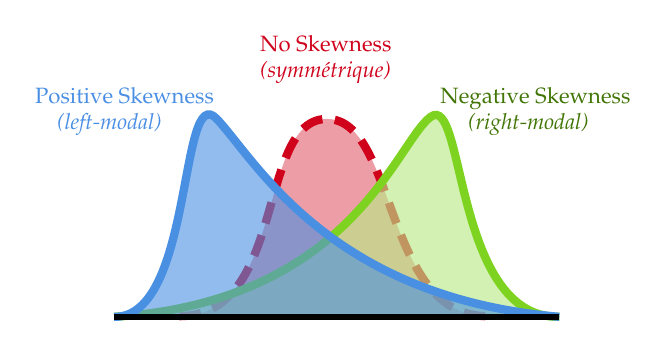
\begin{tikzpicture}[x=0.75pt,y=0.75pt,yscale=-1,xscale=1]
%uncomment if require: \path (0,300); %set diagram left start at 0, and has height of 300

%Curve Lines [id:da2688874623271533] 
\draw [color={rgb, 255:red, 208; green, 2; blue, 27 }  ,draw opacity=1 ][fill={rgb, 255:red, 208; green, 2; blue, 27 }  ,fill opacity=0.39 ][line width=3]  [dash pattern={on 7.88pt off 4.5pt}]  (80.5,138.67) .. controls (132.5,138.67) and (117.5,43.67) .. (151.5,43.67) .. controls (185.5,43.67) and (178.5,139.67) .. (229.5,138.67) ;


%Curve Lines [id:da9147539678395264] 
\draw [color={rgb, 255:red, 126; green, 211; blue, 33 }  ,draw opacity=1 ][fill={rgb, 255:red, 184; green, 233; blue, 134 }  ,fill opacity=0.64 ][line width=3]    (49,139) .. controls (163.5,131.67) and (184.83,55) .. (201.5,42.67) .. controls (218.17,30.33) and (212.5,140) .. (263.5,139) ;


%Curve Lines [id:da8124483083453555] 
\draw [color={rgb, 255:red, 74; green, 144; blue, 226 }  ,draw opacity=1 ][fill={rgb, 255:red, 74; green, 144; blue, 226 }  ,fill opacity=0.6 ][line width=3]    (49,139) .. controls (87.5,139.67) and (80.17,24.33) .. (98.5,43.67) .. controls (116.83,63) and (152.5,129.67) .. (263.5,139) ;

%Straight Lines [id:da7586443312018019] 
\draw [line width=2.25]    (49,139) -- (263.5,139) ;


% Text Node
\draw (151,15) node [scale=0.8,color={rgb, 255:red, 208; green, 2; blue, 27 }  ,opacity=1 ] [align=left] {No Skewness\\\textit{(symmétrique)}};
% Text Node
\draw (252,40) node [scale=0.8,color={rgb, 255:red, 65; green, 117; blue, 5 }  ,opacity=1 ] [align=left] {Negative Skewness\\\textit{ \ \ \ \ (right-modal)}};
% Text Node
\draw (54,40) node [scale=0.8,color={rgb, 255:red, 65; green, 117; blue, 5 }  ,opacity=1 ] [align=left] {\textcolor[rgb]{0.29,0.56,0.89}{Positive Skewness}\\\textit{\textcolor[rgb]{0.29,0.56,0.89}{ \ \ \ \ (left-modal)}}};
\end{tikzpicture}
\end{center}
\end{definitionNOHFILLsub}

\begin{definitionNOHFILLsub}[Kurtosis]
\lfbox[formula]{$\text{Kurtosis}	=	\frac{\mu_{4}}{\sigma^{4}}		=	\frac{\mu'_{4} - 4\mu'_{3}\mu + 6\mu'_{2}\mu^{2} - 3\mu^{4}}{\sigma^{3}}$}.\\

Le kurtosis mesure l'aplatissement d'une distribution et peut aider à juger la vraisemblance qu'une distribution produise des valeurs extrêmes (ou \og \textit{outliers} \fg{}).\\

Le kurtosis de la distribution normale est de 3. On pose qu'il est plus vraisemblable pour une distribution dont le kurtosis supérieur à 3 de produire des valeurs extrêmes.


\begin{center}
\tikzset{every picture/.style={line width=0.75pt}} %set default line width to 0.75pt        
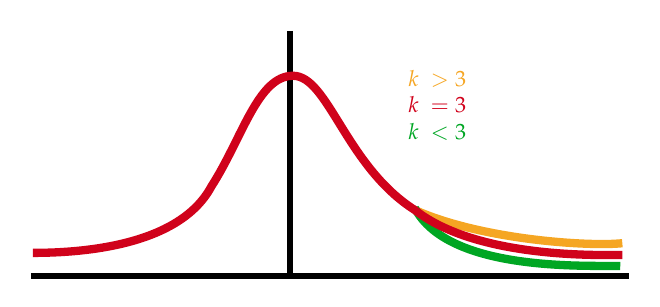
\begin{tikzpicture}[x=0.75pt,y=0.75pt,yscale=-1,xscale=1]
%Curve Lines [id:da18622021578279613] 
\draw [color={rgb, 255:red, 245; green, 166; blue, 35 }  ,draw opacity=1 ][line width=3]    (219.17,255.33) .. controls (252.17,270) and (304.17,273) .. (319.17,271.33) ;
%Curve Lines [id:da37988280307937217] 
\draw [color={rgb, 255:red, 0; green, 166; blue, 35 }  ,draw opacity=1 ][line width=3]    (219.17,254.33) .. controls (235.17,285) and (300.17,282) .. (318.17,282.33) ;
%Straight Lines [id:da5412137305076621] 
\draw [line width=2.25]    (159.17,169) -- (159.17,286) ;
%Curve Lines [id:da11948970250620294] 
\draw [color={rgb, 255:red, 208; green, 2; blue, 27 }  ,draw opacity=1 ][line width=3]    (35.17,276) .. controls (61.17,276) and (106.17,272) .. (121.17,244) .. controls (136.04,220.92) and (143.5,190.67) .. (160.5,190.67) .. controls (177.5,190.67) and (185.87,234.17) .. (219.17,255.33) .. controls (249.17,279) and (309.17,277) .. (319.17,277) ;
%Straight Lines [id:da09355877210927566] 
\draw [line width=2.25]    (34.17,287) -- (322.17,287) ;


% Text Node
\draw (230,206) node [scale=0.8,color={rgb, 255:red, 65; green, 117; blue, 5 }  ,opacity=1 ] [align=left] {$\displaystyle  \begin{array}{{>{\displaystyle}l}}
\textcolor[rgb]{0.96,0.65,0.14}{k\  >3}\\
\textcolor[rgb]{0.82,0.01,0.11}{k\ =3}\\
\textcolor[rgb]{0.0,0.65,0.14}{k\ < 3}
\end{array}$};
\end{tikzpicture}
\end{center}
\end{definitionNOHFILLsub}



\columnbreak
\subsection{Distributions}
\begin{definitionNOHFILLprop}[Loi Pareto]
\begin{rappel_enhanced}[Contexte]
La distribution Pareto est un mélange de deux distributions exponentielles originalement conçue pour étudier des distributions de revenus. 
\end{rappel_enhanced}

\begin{center}
\begin{tabular}{| >{\columncolor{beaublue}}c | >{\columncolor{beaublue}}c  | >{\columncolor{beaublue}}c  |}
\hline\rowcolor{airforceblue} 
\textcolor{white}{\textbf{Notation}}	&	\textcolor{white}{\textbf{Paramètres}}		&	\textcolor{white}{\textbf{Domaine}}	\\\specialrule{0.1em}{0em}{0em} 
$X \sim \text{Pareto}(\alpha, \theta)$	&	$\alpha, \theta	>	0$	&	$x \geq 0$	\\\hline
\end{tabular}
\end{center}

\begin{center}
\begin{tabular}{| >{\columncolor{airforceblue}}m{1cm} | >{\columncolor{beaublue}}m{4cm}  |}
\specialrule{0.1em}{0em}{0em}
\textcolor{white}{$f(x)$}	&	 \[=	\frac{\alpha\theta^{\alpha}}{(x + \theta)^{\alpha + 1}}\]		\\\specialrule{0.1em}{0em}{0em}
\textcolor{white}{$F(x)$}	&	 \[=1 -	\left(\frac{\theta}{x + \theta}\right)^{\alpha}\]		\\\specialrule{0.1em}{0em}{0em}
\end{tabular}
\end{center}

\begin{itemize}
	\item	Si $X \sim \text{Pareto}(\alpha, \theta)$ alors \lfbox[formula]{$Y	=	(X	-	d	|	X	>	d)	\sim \text{Pareto}(\alpha, \theta + d)$}.
\end{itemize}
\end{definitionNOHFILLprop}

\begin{definitionNOHFILLprop}[Loi Beta]
\begin{center}
\begin{tabular}{| >{\columncolor{beaublue}}c | >{\columncolor{beaublue}}c  | >{\columncolor{beaublue}}c  |}
\hline\rowcolor{airforceblue} 
\textcolor{white}{\textbf{Notation}}	&	\textcolor{white}{\textbf{Paramètres}}		&	\textcolor{white}{\textbf{Domaine}}	\\\specialrule{0.1em}{0em}{0em} 
$X \sim \text{Beta}(a, b, \theta)$	&	$a, b	>	0 \text{ et } \theta \geq 0$	&	$x \in [0, \theta]$	\\\hline
\end{tabular}
\end{center}

\begin{center}
\begin{tabular}{| >{\columncolor{airforceblue}}m{1cm} | >{\columncolor{beaublue}}m{4cm}  |}
\specialrule{0.1em}{0em}{0em}
\textcolor{white}{$f(x)$}	&	 \[= \frac{\theta}{\text{B}(a, b)}	\bigg(\frac{x}{\theta}\bigg)^{a - 1} \bigg(1 - \frac{x}{\theta}\bigg)^{b - 1}\]		\\\specialrule{0.1em}{0em}{0em}
\end{tabular}
\end{center}

\begin{itemize}
	\item	$X	\sim \text{Beta}(a = 1, b = 1, \theta) \sim \text{Unif}(0, \theta)$.
	\item	Si $X \sim \text{Unif}(a, b)$ alors  \lfbox[formula]{$(X	|	X	>	d)	\sim \text{Unif}(d, b)$} et \lfbox[formula]{$(X	-	d	|	X	>	d)	\sim \text{Unif}(0, b - d)$}.
\end{itemize}
\end{definitionNOHFILLprop}

\begin{definitionNOHFILLprop}[Loi Gamma]
\begin{center}
\begin{tabular}{| >{\columncolor{beaublue}}c | >{\columncolor{beaublue}}c  | >{\columncolor{beaublue}}c  |}
\hline\rowcolor{airforceblue} 
\textcolor{white}{\textbf{Notation}}	&	\textcolor{white}{\textbf{Paramètres}}		&	\textcolor{white}{\textbf{Domaine}}	\\\specialrule{0.1em}{0em}{0em} 
$X \sim \text{Gamma}(\alpha, \theta)$	&	$\alpha, \theta > 0$	&	$x \geq	0$	\\\hline
\end{tabular}
\end{center}

\begin{center}
\begin{tabular}{| >{\columncolor{airforceblue}}m{1cm} | >{\columncolor{beaublue}}m{4cm}  |}
\specialrule{0.1em}{0em}{0em}
\textcolor{white}{$f(x)$}	&	 \[= \frac{x^{\alpha - 1} \textrm{e}^{-x/\theta}}{\Gamma(\alpha)\theta^{\alpha}}\]		\\\specialrule{0.1em}{0em}{0em}
\end{tabular}
\end{center}

\begin{itemize}
	\item	On appelle $\theta$ la moyenne et $\lambda	=	\frac{1}{\theta}$ le paramètre de fréquence (\og \textit{rate} \fg{}).
	\item	Soit n v.a. indépendantes \lfbox[conditions]{$X_{i}	\sim \text{Gamma}(\alpha_{i}, \theta)$} alors \lfbox[formula]{$\sum_{i = 1}^{n} X_{i} \sim \text{Gamma}(\sum_{i = 1}^{n} \alpha_{i}, \theta)$}.
	\item	Soit n v.a. indépendantes \lfbox[conditions]{$X_{i}	\sim \text{Exp}(\lambda_{i})$} alors \lfbox[formula]{$Y	=	\min(X_{1}, \dots, X_{n})	\sim	\text{Exp}(\frac{1}{\sum_{i = 1}^{n} \lambda_{i})}$}.
	\item	Si $X \sim \text{Exp}(\theta)$ alors \lfbox[formula]{$(X	-	d	|	X	>	d)	\sim \text{Exp}(\theta)$}.
\end{itemize}
\end{definitionNOHFILLprop}


\columnbreak
\subsection{Transformation}
\begin{definitionNOHFILLsub}[Changement d'échelle pour des v.a. continues]
Toutes les distributions continues (sauf pour la lognormale, l'inverse gaussienne et la log-t) ont $\theta$ comme paramètre d'échelle. Alors, multiplier la v.a. par une constante $c$ change uniquement le paramètre $\theta^{\ast}	=	c\theta$.
\end{definitionNOHFILLsub}

\begin{algo2}[Trouver la PDF d'une v.a. transformée]
Soit $n$ v.a. $X_{1}, \dots, X_{n}$ que l'on veut transformer en $n$ autres variables aléatoires $W_{1}	=	g_{1}(X_{1}, \dots, X_{n}), \dots, W_{n}	=	g_{n}(X_{1}, \dots, X_{n})$.
\begin{enumerate}[label	=	\circled{\arabic*}{trueblue}]
	\item	Trouver les inverses des équations de la transformation : 
		\begin{align*}
		x_{1}	
		&=	g^{-1}_{1}(w_{1}, \dots, w_{n})	\\
		\vdots	\\
		x_{n}	
		&=	g^{-1}_{n}(w_{1}, \dots, w_{n})	
		\end{align*}
	\item	Calculer le déterminant de la matrice Jacobienne $J$ : 
		\begin{align*}
		J
		&=	\det \begin{bmatrix}
		\deriv{w_{1}}{x_{1}}	&	\hdots	&	\deriv{w_{n}}{x_{1}}	\\
		\vdots	&	\ddots	&	\vdots	\\
		\deriv{w_{1}}{x_{n}}		&	\hdots	&	\deriv{w_{n}}{x_{n}}
		\end{bmatrix}
		\end{align*}
	\item	Trouver la fonction de densité conjointe avec 
\end{enumerate}
\lfbox[formula]{$f_{W_{1}, \dots, W_{n}}(w_{1}, \dots, w_{n})	=	f_{X_{1}, \dots, X_{n}}\left(g^{-1}_{1}(w_{1}, \dots, w_{n}), \dots, g^{-1}_{n}(w_{1}, \dots, w_{n})\right) |J|$}.

\paragraph{Note}	Dans le cas univarié, \lfbox[formula]{$f_{W}(w)	=	f_{X}\left(g^{-1}(w)\right) \left|\deriv{w}{g^{-1}(w)}\right|$}.
\end{algo2}


\columnbreak
\subsection{Queues de distributions}
\begin{rappel_enhanced}[Contexte]
Si une distribution a une queue de droite qui est lourde, \og \textit{thick} \fg{} ou \og \textit{fat} \fg{}, alors elle a des probabilités élevées de pertes extrêmes.
\end{rappel_enhanced}

En situation d'examen nous ne pouvons pas visuellement évaluer la queue et donc nous utilisons un des 4 tests suivants :
\begin{definitionGENERAL}{Nombre de moments (positifs) qui existent}[\circled{1}{trueblue}]
\textit{Plus} la queue est \textbf{\textbf{\textcolor{teal}{lourde}}}, \textit{\textcolor{teal}{moins}} il y a de moments qui existent.\\

\begin{itemize}
	\item	Il devient de moins en moins probable que l'intégrale de $x^{k}f(x)$ va converger.
\end{itemize}
\end{definitionGENERAL}

\begin{definitionGENERAL}{Ratio des fonctions de survie (ou PDF)}[\circled{2}{trueblue}]
\textit{Plus} la queue est \textbf{\textbf{\textcolor{teal}{lourde}}}, \textit{\textcolor{teal}{plus}} la fonction de \textcolor{teal}{survie va tendre vers 0 \textit{\textbf{lentement}}}.\\

\begin{itemize}
	\item	Si $\limz{x}{\infty} \frac{S_{1}(x)}{S_{2}(x)}	=	0$ alors $X_{1}$ a une queue plus légère que $X_{2}$, et vice-versa si la limite tend vers $\infty$.
	\item	Par la règle de l'hôpital, ceci est équivalent pour le ratio des PDF.
\end{itemize}
\end{definitionGENERAL}

\begin{definitionGENERAL}{Fonctions de hasard}[\circled{3}{trueblue}]
Si la \textcolor{teal}{fonction de hasard} est \textit{\textcolor{teal}{décroissante}}, il y a une probabilité plus élevée de pertes extrêmes et donc une queue \textit{\textbf{\textcolor{teal}{lourde}}}.
\end{definitionGENERAL}

\begin{definitionGENERAL}{CTEs (ou quantiles)}[\circled{4}{trueblue}]
\textbf{\textit{\textcolor{teal}{Plus}}} le \textcolor{teal}{CTE (ou les quantiles) est large}, plus les montants de pertes extrêmes sont larges et donc \textit{plus} la queue est \textit{\textbf{\textcolor{teal}{lourde}}}.
\end{definitionGENERAL}



\pagebreak
\section{Estimations et types de données}
\subsection{Distributions empiriques}
\begin{distributions}[Notation]
\begin{description}
	\item[$X$]	Variable aléatoire de perte;
	\item[$\theta$]	Paramètre de la distribution de $X$;
		\begin{itemize}[leftmargin = *]
		\item	Le paramètre peut être un scalaire $\theta$ ou un vecteur $\bm{\theta}$;
		\item	Par exemple, pour une loi Gamma $\bm{\theta} = \{\alpha,	\beta\}$;
		\item	Pour simplifier la notation, on le traite comme un scalaire $\theta$.
		\end{itemize}
	\item[$F_{X}(x; \theta)$]	Fonction de répartition de $X$ avec paramètre $\theta$;
		\begin{itemize}[leftmargin = *]
		\item	Pour simplifier la notation, on écrit $F(x; \theta)$ sauf s'il faut être plus spécifique.
		\end{itemize}
	\item[$f_{X}(x; \theta)$]	Fonction de densité de $X$ avec paramètre $\theta$;
		\begin{itemize}[leftmargin = *]
		\item	Pour simplifier la notation, on écrit $f(x; \theta)$ sauf s'il faut être plus spécifique.
		\end{itemize}
	\item[$\{X_{1}, \dots, X_{n}\}$]	Échantillon aléatoire de $n$ observations de $X$;
	\item[$\hat{\theta}$]	Estimateur de $\theta$ établit avec l'échantillon aléatoire $\{X_{1}, \dots, X_{n}\}$;
	\item[$F(x; \hat{\theta})$]	Estimation \textit{paramétrique} de la fonction de répartition de $X$;
	\item[$f(x; \hat{\theta})$]	Estimation \textit{paramétrique} de la fonction de densité de $X$;
\end{description}
\end{distributions}
\begin{itemize}[leftmargin = *]
	\item	Si $\theta$ est connu, la distribution de $X$ est complètement spécifiée;\\
			En pratique, $\theta$ est inconnu et doit être estimé avec les données observées.
	\item	On peut estimer $F_{X}(x)$ et $f_{X}(x)$ directement pour toute valeur $x$ sans présumer une forme paramétrique;\\
			Par exemple, un histogramme est une estimation \textit{non-paramétrique}.
\end{itemize}


\columnbreak
\subsection{Données complètes}
\begin{distributions}[Notation]
\begin{description}
	\item[$X$]	Variable d'intérêt (e.g., la durée de vie ou la perte);
	\item[$\{X_{1}, \dots, X_{n}\}$]	Valeurs de $X$ pour n individus;
	\item[$\{x_{1}, \dots, x_{n}\}$]	$n$ valeurs observées de l'échantillon;
		\begin{itemize}[leftmargin = *]
		\item	Il peut y avoir des valeurs dupliquées dans les valeurs observées.
		\end{itemize}
	\item[$0	<	y_{1}	<	\hdots	<	y_{m}$]	$m$ valeurs distincts où \icbox[red][palechestnut]{$m \leq n$};
	\item[$w_{j}$]	Nombre de fois que la valeur $y_{j}$ apparaît dans l'échantillon pour \icbox[red][palechestnut]{$j = 1, \dots, m$};
		\begin{itemize}[leftmargin = *]
		\item	Il s'ensuit que \icbox[red][palechestnut]{$\sumz{m}{j = 1}w_{j}	=	n$};
		\item	Pour des données de mortalité, $w_{j}$ individus décèdent à l'âge $y_{j}$;
		\item	Si tous les individus sont observés de la naissance jusqu'à la mort c'est un \og \textit{complete individual data set} \fg{}.
		\end{itemize}
	\item[$r_{j}$]	\og \textit{risk set} \fg{} au \textit{temps} $y_{j}$;
		\begin{itemize}[leftmargin = *]
		\item	Le nombre d'individus exposés à la possibilité de mourir au temps $y_{j}$;
		\item	Par exemple, $r_{1}	=	n$ car tous les individus sont exposés à la risque de décéder juste avant le temps $y_{1}$;
		\item	On déduit que \icbox[red][palechestnut]{$r_{j}	=	\sumz{m}{i = j}w_{i}$}, alias le nombre d'individus qui survivent juste avant le temps $y_{j}$.
		\end{itemize}
\end{description}
\end{distributions}

\columnbreak
\subsection{Données incomplètes}

\begin{rappel_enhanced}[Exemple]
Soit une étude sur le nombre d'années nécessaire pour obtenir un diplôme universitaire. L'étude commence cette année et tient compte de tous les étudiants présentement inscrits, ainsi que ceux qui vont s'inscrire au courant de l'étude. Tous les étudiants sont observés jusqu'à la fin de l'étude et on note le nombre d'années nécessaire pour ceux qui complètent leurs diplômes. \\

Si un étudiant a commencé son cursus scolaire avant l'étude et suit présentement des cours, le chercheur a de l'information sur le nombre d'années qu'il a déjà investi. Cependant, d'autres étudiants qui se sont inscrits en même temps, mais ont cessé leurs études ne seront pas observés dans cet échantillon. Alors, l'individu est observé d'une population \lfbox[imphl]{\textbf{tronquée à la gauche}} puisque l'information sur les étudiants qui ont quitté l'université avant le début de l'étude n'est \textit{pas disponible}.\\

Si un étudiant n'est pas encore diplômé lorsque l'étude prend fin, le chercheur ne peut pas savoir combien d'années supplémentaire seront nécessaires. Cet individu fait donc partie d'une population \lfbox[imphl]{\textbf{censurée à la droite}} puisque le chercheur a de l'information \textit{partielle} (le nombre d'années minimale) sans savoir le nombre exact.
\end{rappel_enhanced}

\begin{distributions}[Notation]
\begin{description}
	\item[$d_{i}$]	État de troncature de l'individu $i$ de l'échantillon;
		\begin{itemize}[leftmargin = *]
		\item	$d_{i}	=	0$ s'il n'y a pas de troncature;
		\item	Par exemple, un étudiant à commencé son programme universitaire $d_{i}$ années avant le début de l'étude.
		\end{itemize}
	\item[$x_{i}$]	Temps de "survie" de l'individu $i$;
		\begin{itemize}[leftmargin = *]
		\item	Par exemple, le nombre d'années avant d'obtenir son diplôme;
		\item	Si l'étude prend fin avant que $x_{i}$ soit observé, on dénote le temps de survie jusqu'à ce moment \icbox{$u_{i}$};
		\item	Donc chaque individu a \textit{soit} une valeur $x_{i}$ \underline{ou} $u_{i}$ mais \textit{pas les deux}.
		\end{itemize}
\end{description}
\end{distributions}

\columnbreak
\subsection{Données groupées}
\begin{distributions}[Notation]
\begin{description}
	\item[]	$(c_{0}, c_{1}], (c_{1}, c_{2}], \dots, (c_{k - 1}, c_{k}]$	$k$ intervalles regroupant les observations;
	\item[$0	\leq	c_{0}	<	c_{1}	<	\hdots	<	c_{k}$]	Extrémités des $k$ intervalles;
	\item[$n$]	Nombre d'observations de $x_{i}$ dans l'échantillon;
	\item[$n_{j}$]	Nombre d'observations de $x_{i}$ dans l'intervalle $(c_{j - 1}, c_{j}]$;
		\begin{itemize}[leftmargin = *]
		\item	Il s'ensuit que \icbox[red][palechestnut]{$\sumz{k}{j = 1}n_{j}	=	n$}.
		\end{itemize}
	\item[$r_{j}$]	\og \textit{risk set} \fg{} de l'intervalle $(c_{j - 1}, c_{j}]$ lorsque les données sont complètes;
		\begin{itemize}[leftmargin = *]
		\item	Il s'ensuit que \icbox[red][palechestnut]{$r_{j}	=	\sumz{k}{i = j}n_{i}$}.
		\end{itemize}
\end{description}
\end{distributions}


\columnbreak
\section{Applications en assurance}
\begin{distributions}[Notation]
\begin{description}
	\item[$X$]	Variable aléatoire du montant de perte.
\end{description}
\end{distributions}


\subsection{Limite de police}
\begin{definitionNOHFILL}[Limite de police]
Une \textbf{limite de police} \lfbox[formula]{$u$} est le montant maximal qu'un assureur va payer pour une perte.\\


Visuellement : 
\begin{center}


\tikzset{every picture/.style={line width=0.75pt}} %set default line width to 0.75pt        

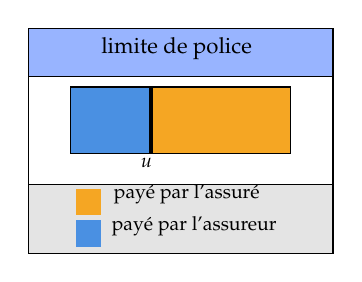
\begin{tikzpicture}[x=0.75pt,y=0.75pt,yscale=-1,xscale=1]
%uncomment if require: \path (0,154); %set diagram left start at 0, and has height of 154

%Shape: Rectangle [id:dp02803686274972339] 
\draw  [fill={rgb, 255:red, 255; green, 255; blue, 255 }  ,fill opacity=1 ] (311,17.67) -- (457.83,17.67) -- (457.83,126) -- (311,126) -- cycle ;
%Shape: Rectangle [id:dp6650428705496374] 
\draw  [fill={rgb, 255:red, 228; green, 228; blue, 228 }  ,fill opacity=1 ] (311,93) -- (457.83,93) -- (457.83,126) -- (311,126) -- cycle ;
%Shape: Rectangle [id:dp011257611005494716] 
\draw  [fill={rgb, 255:red, 152; green, 180; blue, 255 }  ,fill opacity=1 ] (311,17.67) -- (457.83,17.67) -- (457.83,41) -- (311,41) -- cycle ;
%Shape: Rectangle [id:dp9403819194026608] 
\draw  [draw opacity=0][fill={rgb, 255:red, 245; green, 166; blue, 35 }  ,fill opacity=1 ] (370,46) -- (437.5,46) -- (437.5,78) -- (370,78) -- cycle ;
%Shape: Rectangle [id:dp48392000225673093] 
\draw  [draw opacity=0][fill={rgb, 255:red, 74; green, 144; blue, 226 }  ,fill opacity=1 ] (331.33,46) -- (370,46) -- (370,78) -- (331.33,78) -- cycle ;
%Shape: Rectangle [id:dp7277326812364118] 
\draw   (331.33,46) -- (437.5,46) -- (437.5,78) -- (331.33,78) -- cycle ;
%Straight Lines [id:da8740810297553647] 
\draw [line width=1.5]    (370,46) -- (370,78) ;
%Shape: Rectangle [id:dp4533678374731276] 
\draw  [draw opacity=0][fill={rgb, 255:red, 245; green, 166; blue, 35 }  ,fill opacity=1 ] (333.83,94.97) -- (346.17,94.97) -- (346.17,107.7) -- (333.83,107.7) -- cycle ;
%Shape: Rectangle [id:dp2562930482964858] 
\draw  [draw opacity=0][fill={rgb, 255:red, 74; green, 144; blue, 226 }  ,fill opacity=1 ] (333.83,110.13) -- (346.17,110.13) -- (346.17,122.87) -- (333.83,122.87) -- cycle ;

% Text Node
\draw (344.92,20.67) node [anchor=north west][inner sep=0.75pt]   [align=left] {{\footnotesize limite de police}};
% Text Node
\draw (351,91.83) node [anchor=north west][inner sep=0.75pt]   [align=left] {{\scriptsize payé par l'assuré}};
% Text Node
\draw (350,107) node [anchor=north west][inner sep=0.75pt]   [align=left] {{\scriptsize payé par l'assureur}};
% Text Node
\draw (364,79) node [anchor=north west][inner sep=0.75pt]  [font=\scriptsize] [align=left] {$\displaystyle u$};


\end{tikzpicture}
\end{center}
\end{definitionNOHFILL}

\begin{definitionNOHFILLsub}[Montant de perte limité]
La variable aléatoire du \textbf{montant de perte limité} \lfbox[formula]{$X \wedge u$} correspond au montant du paiement de l'assureur pour une police d'assurance ayant une limite de $u$ :

\begin{align*}
	X \wedge u
	&=	\begin{cases}
		X,	&	X < u	\\
		u,	&	X \geq u	\\
		\end{cases}
\end{align*}
\begin{itemize}
	\item	Il s'ensuit que \lfbox[formula]{$X \wedge d	=	\min(X; d)$}.
\end{itemize}

Visuellement : 

\begin{center}
\tikzset{every picture/.style={line width=0.75pt}} %set default line width to 0.75pt        
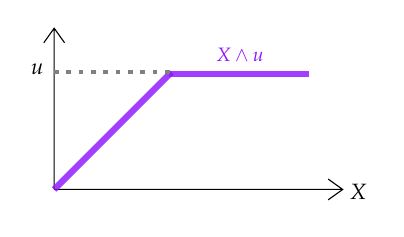
\begin{tikzpicture}[x=0.75pt,y=0.75pt,yscale=-1,xscale=1]
%uncomment if require: \path (0,174); %set diagram left start at 0, and has height of 174

%Shape: Axis 2D [id:dp6598259573253495] 
\draw  (313.5,139) -- (452.5,139)(313.5,61.33) -- (313.5,139) -- cycle (445.5,134) -- (452.5,139) -- (445.5,144) (308.5,68.33) -- (313.5,61.33) -- (318.5,68.33)  ;
%Straight Lines [id:da2579967683196891] 
\draw [color={rgb, 255:red, 142; green, 19; blue, 254 }  ,draw opacity=0.82 ][line width=2.25]    (313.5,139) -- (370,82.5) ;
%Straight Lines [id:da18638822683919853] 
\draw [color={rgb, 255:red, 142; green, 19; blue, 254 }  ,draw opacity=0.82 ][line width=2.25]    (369,83.5) -- (436.46,83.5) ;
%Straight Lines [id:da08876956095236466] 
\draw [color={rgb, 255:red, 128; green, 128; blue, 128 }  ,draw opacity=1 ][line width=1.5]  [dash pattern={on 1.69pt off 2.76pt}]  (313.5,82.5) -- (370,82.5) ;

% Text Node
\draw (460,140) node  [font=\footnotesize] [align=left] {$\displaystyle X$};
% Text Node
\draw (403,74) node  [font=\scriptsize,color={rgb, 255:red, 144; green, 19; blue, 254 }  ,opacity=1 ] [align=left] {$\displaystyle X\land u$};
% Text Node
\draw (301,77) node [anchor=north west][inner sep=0.75pt]  [font=\footnotesize] [align=left] {$\displaystyle u$};


\end{tikzpicture}
\end{center}
\end{definitionNOHFILLsub}

\begin{definitionNOHFILLsub}[L'espérance limitée du montant de perte]
\textbf{L'espérance limitée du montant de perte} \lfbox[formula]{$\text{E}[X \wedge u]$} correspond à l'espérance du paiement de l'assureur pour une police d'assurance ayant une limite de $u$ :

\begin{align*}
	\text{E}[X \wedge u]	
	&=	\int_{0}^{u} x f(x) dx + u S(u)
\end{align*}
\end{definitionNOHFILLsub}


\columnbreak
\subsection{Déductibles}
\begin{definitionNOHFILL}[Déductible]
Le \textbf{déductible d'une police} est le montant que l'assuré doit payer de sa poche avant que l'assureur débourse pour une perte. \\

Il y a 2 types de déductibles : 
\begin{description}
	\item[déductible ordinaire]	Une fois que le montant de perte surpasse le déductible, l'assureur va payer le montant de la perte \textbf{en excès du déductible}.
	\item[déductible de franchise]	Une fois que le montant de perte surpasse le déductible, l'assureur va payer le montant \textbf{total} de la perte.
\end{description}

Par défaut, on suppose le déductible ordinaire.\\

Visuellement :

\begin{center}
\tikzset{every picture/.style={line width=0.75pt}} %set default line width to 0.75pt        
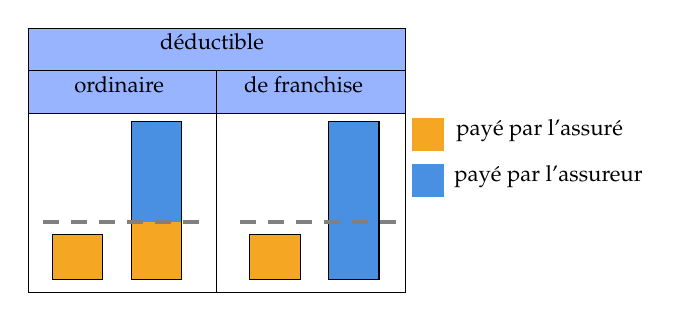
\begin{tikzpicture}[x=0.75pt,y=0.75pt,yscale=-1,xscale=1]
%uncomment if require: \path (0,217); %set diagram left start at 0, and has height of 217

%Shape: Rectangle [id:dp588617566986505] 
\draw  [draw opacity=0][fill={rgb, 255:red, 245; green, 166; blue, 35 }  ,fill opacity=1 ] (128.75,134.92) -- (128.75,113.33) -- (152.99,113.33) -- (152.99,134.92) -- cycle ;
%Shape: Rectangle [id:dp003856682054647287] 
\draw   (128.75,134.92) -- (128.75,113.33) -- (152.99,113.33) -- (152.99,134.92) -- cycle ;
%Shape: Rectangle [id:dp700556830555261] 
\draw  [draw opacity=0][fill={rgb, 255:red, 245; green, 166; blue, 35 }  ,fill opacity=1 ] (301.83,56.92) -- (317.17,56.92) -- (317.17,72.75) -- (301.83,72.75) -- cycle ;
%Shape: Rectangle [id:dp7089085688842631] 
\draw  [draw opacity=0][fill={rgb, 255:red, 74; green, 144; blue, 226 }  ,fill opacity=1 ] (301.83,79) -- (317.33,79) -- (317.33,95) -- (301.83,95) -- cycle ;
%Shape: Rectangle [id:dp40057299526008183] 
\draw  [draw opacity=0][fill={rgb, 255:red, 74; green, 144; blue, 226 }  ,fill opacity=1 ] (166.75,107.14) -- (166.75,58.67) -- (190.99,58.67) -- (190.99,107.14) -- cycle ;
%Shape: Rectangle [id:dp7752631736808828] 
\draw  [draw opacity=0][fill={rgb, 255:red, 245; green, 166; blue, 35 }  ,fill opacity=1 ] (166.75,134.92) -- (166.75,107.14) -- (190.99,107.14) -- (190.99,134.92) -- cycle ;
%Shape: Rectangle [id:dp8322518421090499] 
\draw   (166.75,134.92) -- (166.75,58.67) -- (190.99,58.67) -- (190.99,134.92) -- cycle ;
%Straight Lines [id:da21204533122634284] 
\draw [color={rgb, 255:red, 128; green, 128; blue, 128 }  ,draw opacity=1 ][line width=1.5]  [dash pattern={on 5.63pt off 4.5pt}]  (124.17,107) -- (200.17,107) ;
%Shape: Rectangle [id:dp10210761313509842] 
\draw  [draw opacity=0][fill={rgb, 255:red, 245; green, 166; blue, 35 }  ,fill opacity=1 ] (223.75,134.92) -- (223.75,113.33) -- (247.99,113.33) -- (247.99,134.92) -- cycle ;
%Shape: Rectangle [id:dp1422285500093443] 
\draw   (223.75,134.92) -- (223.75,113.33) -- (247.99,113.33) -- (247.99,134.92) -- cycle ;
%Shape: Rectangle [id:dp3614273531351382] 
\draw  [draw opacity=0][fill={rgb, 255:red, 74; green, 144; blue, 226 }  ,fill opacity=1 ] (261.75,134.92) -- (261.75,58.67) -- (285.99,58.67) -- (285.99,134.92) -- cycle ;
%Shape: Rectangle [id:dp4016556775232154] 
\draw   (261.75,134.92) -- (261.75,58.67) -- (285.99,58.67) -- (285.99,134.92) -- cycle ;
%Straight Lines [id:da9540437083363307] 
\draw [color={rgb, 255:red, 128; green, 128; blue, 128 }  ,draw opacity=1 ][line width=1.5]  [dash pattern={on 5.63pt off 4.5pt}]  (219.17,107) -- (295.17,107) ;
%Shape: Rectangle [id:dp7792912132142298] 
\draw   (117,43) -- (207.83,43) -- (207.83,141.33) -- (117,141.33) -- cycle ;
%Shape: Rectangle [id:dp19600907651515787] 
\draw  [fill={rgb, 255:red, 152; green, 180; blue, 255 }  ,fill opacity=1 ] (117,34.33) -- (207.83,34.33) -- (207.83,54.85) -- (117,54.85) -- cycle ;
%Shape: Rectangle [id:dp25767783018946355] 
\draw   (207.83,43) -- (298.67,43) -- (298.67,141.33) -- (207.83,141.33) -- cycle ;
%Shape: Rectangle [id:dp6656766828727914] 
\draw  [fill={rgb, 255:red, 152; green, 180; blue, 255 }  ,fill opacity=1 ] (207.83,34.33) -- (298.67,34.33) -- (298.67,54.85) -- (207.83,54.85) -- cycle ;
%Shape: Rectangle [id:dp932544307028238] 
\draw  [fill={rgb, 255:red, 152; green, 180; blue, 255 }  ,fill opacity=1 ] (117,13.82) -- (298.67,13.82) -- (298.67,34.33) -- (117,34.33) -- cycle ;

% Text Node
\draw (137.92,35.76) node [anchor=north west][inner sep=0.75pt]   [align=left] {{\footnotesize ordinaire}};
% Text Node
\draw (322,56.33) node [anchor=north west][inner sep=0.75pt]   [align=left] {{\footnotesize payé par l'assuré}};
% Text Node
\draw (321,78.5) node [anchor=north west][inner sep=0.75pt]   [align=left] {{\footnotesize payé par l'assureur}};
% Text Node
\draw (219.75,35.76) node [anchor=north west][inner sep=0.75pt]   [align=left] {{\footnotesize de franchise}};
% Text Node
\draw (179.33,15.05) node [anchor=north west][inner sep=0.75pt]   [align=left] {{\footnotesize déductible}};


\end{tikzpicture}
\end{center}
\end{definitionNOHFILL}


\subsubsection{Déductible ordinaire}
\begin{definitionNOHFILLsub}[Montant de perte avec un déductible \textbf{ordinaire}]
La variable aléatoire du montant de perte pour une police ayant un \textbf{déductible ordinaire} de $d$. \\

\begin{minipage}[ht]{0.5\columnwidth}
\begin{center}
	Assureur
\end{center}
\begin{align*}
	(X - d)_{+}
	&=	\begin{cases}
		0,	  	&	X \leq d	\\
		X - d,	&	X > d	
		\end{cases}
\end{align*}
\end{minipage}%
\begin{minipage}[ht]{0.5\columnwidth}
\begin{center}
	Assuré
\end{center}
\begin{align*}
	X \wedge d
	&=	\begin{cases}
		X,  &	X < d	\\
		d,	&	X \geq d	
		\end{cases}
\end{align*}
\end{minipage}

\

\begin{itemize}
	\item	Il s'ensuit que \lfbox[formula]{$(X - d)_{+}	=	\max(X - d; 0)$}.
	\item	On observe que le montant de perte est la somme des contributions \lfbox[conditions]{$X	=	X \wedge d + (X - d)_{+}$}.
\end{itemize}

Visuellement :
\begin{center}
\tikzset{every picture/.style={line width=0.75pt}} %set default line width to 0.75pt        
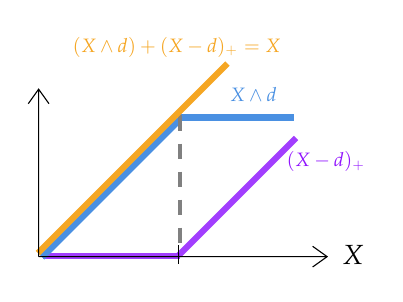
\begin{tikzpicture}[x=0.75pt,y=0.75pt,yscale=-1,xscale=1]
%uncomment if require: \path (0,155); %set diagram left start at 0, and has height of 155

%Straight Lines [id:da2658768489155079] 
\draw [color={rgb, 255:red, 142; green, 19; blue, 254 }  ,draw opacity=0.82 ][line width=2.25]    (429,118.33) -- (485.5,61.83) ;
%Straight Lines [id:da11698723071359618] 
\draw [color={rgb, 255:red, 142; green, 19; blue, 254 }  ,draw opacity=0.82 ][line width=2.25]    (363.54,118.62) -- (429.67,118.62) ;
%Straight Lines [id:da326418494508391] 
\draw [color={rgb, 255:red, 74; green, 144; blue, 226 }  ,draw opacity=1 ][line width=2.25]    (363.17,119.33) -- (429.5,53) ;
%Straight Lines [id:da8149304204229495] 
\draw [color={rgb, 255:red, 74; green, 144; blue, 226 }  ,draw opacity=1 ][line width=2.25]    (429.5,52) -- (484.5,52) ;
%Straight Lines [id:da6292319909047852] 
\draw [color={rgb, 255:red, 128; green, 128; blue, 128 }  ,draw opacity=1 ][line width=1.5]  [dash pattern={on 5.63pt off 4.5pt}]  (429.5,51) -- (429.5,117.62) ;
%Straight Lines [id:da12597396522940518] 
\draw    (429,122.33) -- (429,113.33) ;
%Straight Lines [id:da048934088668804776] 
\draw [color={rgb, 255:red, 245; green, 166; blue, 35 }  ,draw opacity=1 ][line width=2.25]    (361.17,117.33) -- (452.5,26) ;
%Shape: Axis 2D [id:dp3636642155394634] 
\draw  (361.5,119) -- (500.5,119)(361.5,38.33) -- (361.5,119) -- cycle (493.5,114) -- (500.5,119) -- (493.5,124) (356.5,45.33) -- (361.5,38.33) -- (366.5,45.33)  ;

% Text Node
\draw (513,118) node   [align=left] {$\displaystyle X$};
% Text Node
\draw (500,73) node  [font=\scriptsize,color={rgb, 255:red, 144; green, 19; blue, 254 }  ,opacity=1 ] [align=left] {$\displaystyle ( X-d)_{+}$};
% Text Node
\draw (465,41) node  [font=\scriptsize,color={rgb, 255:red, 74; green, 144; blue, 226 }  ,opacity=1 ] [align=left] {$\displaystyle X\land d$};
% Text Node
\draw (428,18) node  [font=\scriptsize,color={rgb, 255:red, 245; green, 166; blue, 35 }  ,opacity=1 ] [align=left] {$\displaystyle ( X\land d) +( X-d)_{+} =X$};


\end{tikzpicture}
\end{center}
\end{definitionNOHFILLsub}

\begin{definitionNOHFILLsub}[L'espérance du montant de perte avec un déductible ordinaire]
\textbf{L'espérance du montant de perte}, pour l'assureur, \textbf{avec un déductible \textit{ordinaire}} \lfbox[formula]{$\text{E}[(X - d)_{+}]$} correspond à :

\begin{align*}
	\text{E}[(X - d)_{+}]
	&=	\int_{d}^{\infty} (x - d) f(x) dx
\end{align*}
\end{definitionNOHFILLsub}

\begin{definitionNOHFILLprop}[\og \textit{Loss Elimination Ratio (LER)} \fg{}]
Le \og \textit{Loss Elimination Ratio (LER)} \fg{} évalue combien qu'épargne l'assureur en imposant un déductible \textit{ordinaire} de $d$,
\lfbox[formula]{$LER	=	\frac{\text{E}[X \wedge d]}{\text{E}[X]}$}.
\end{definitionNOHFILLprop}


\subsubsection{\og \textit{payment \textbf{per loss}} \fg{} et \og \textit{payment \textbf{per payment}} \fg{}}
\begin{distributions}[Notation]
\begin{description}
	\item[$Y^{L}$]	Montant de perte.
		\begin{itemize}
		\item	\og \textit{payment per \textbf{l}oss} \fg{}
		\end{itemize}
	\item[$Y^{P}$]	Montant de paiement.
		\begin{itemize}
		\item	\og \textit{payment per \textbf{p}ayment} \fg{}
		\end{itemize}
\end{description}
\end{distributions}

\begin{description}
	\item[$\text{E}\lbrack Y^{L} \rbrack$]	Montant espéré de paiement \textbf{par perte \textit{subie}}.
	\item[$\text{E}\lbrack Y^{P}\rbrack$]	Montant espéré de paiement \textbf{par paiement \textit{effectué}}.
		\begin{itemize}
		\item	Par exemple, lorsqu'une police a un déductible, les pertes dont le coût est inférieur au déductible ne seront pas reportées à l'assureur.
		\item	Le montant de paiement est donc le montant que l'assureur va payer conditionnel à ce qu'il y ait un paiement.
		\item	Il s'ensuit que \lfbox[conditions]{$\text{E}[Y^{L}] \geq \text{E}[Y^{L}]$}.
		\end{itemize}
\end{description}


Pour un déductible ordinaire de $d$, 

\begin{minipage}[ht]{0.5\columnwidth}
\begin{align*}
	\text{E}[Y^{L}]
	&=	\text{E}[(X - d)_{+}]
\end{align*}
\end{minipage}%
\begin{minipage}[ht]{0.5\columnwidth}
\begin{align*}
	\text{E}[Y^{P}]
	&=	\text{E}[X - d | X > d]
\end{align*}
\end{minipage}

\begin{itemize}
	\item	On trouve que \lfbox[formula]{$\text{E}[Y^{P}]	=	\frac{\text{E}[Y^{L}]}{S(d)}$}.
	\item	Également, le montant espéré de paiement par paiement effectué \textit{est} la fonction d'excès moyen \lfbox[formula]{$\text{E}[Y^{P}]	=	e(d)$}.
	\item	Si la police d'assurance comporte uniquement une limite, \lfbox[conditions]{$Y^{P}	=	Y^{L}$}.
\end{itemize}

\

\textbf{Relations pour quelques distributions} :
\begin{center}
\begin{tabular}{| >{\columncolor{beaublue}}c | >{\columncolor{beaublue}}c  |}
\hline\rowcolor{airforceblue} 
\textcolor{white}{$X$}	&	\textcolor{white}{$(X - d | X > d)$}		\\\specialrule{0.1em}{0em}{0em} 
$\text{Exp}(\theta)$&	$\text{Exp}(\theta)$	\\\hline
$\text{Unif}(a, b)$&	$\text{Unif}(0, b - d)$	\\\hline
$\text{Pareto}(\alpha, \theta)$&	$\text{Pareto}(\alpha, \theta + d)$	\\\hline
$\text{Beta}(1, b, \theta)$&	$\text{Beta}(1, b, \theta - d)$	\\\hline
\end{tabular}
\end{center}


\subsubsection{Déductible de franchise}
\begin{definitionNOHFILLsub}[Montant de perte avec un déductible \textbf{de franchise}]
La variable aléatoire du montant de perte pour une police ayant un \textbf{déductible de franchise} de $d$. 

\begin{align*}
	(X | X > d)
	&=	\begin{cases}
		0,	  	&	X \leq d	\\
		X,	&	X > d	
		\end{cases}
\end{align*}

Visuellement : 
\begin{center}
\tikzset{every picture/.style={line width=0.75pt}} %set default line width to 0.75pt        
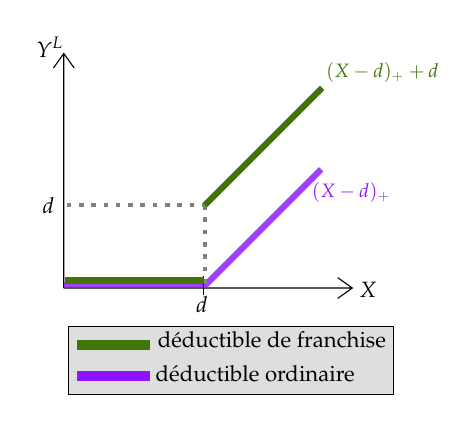
\begin{tikzpicture}[x=0.75pt,y=0.75pt,yscale=-1,xscale=1]
%uncomment if require: \path (0,253); %set diagram left start at 0, and has height of 253

%Shape: Axis 2D [id:dp399710789539935] 
\draw  (351.5,163) -- (490.5,163)(351.5,50) -- (351.5,163) -- cycle (483.5,158) -- (490.5,163) -- (483.5,168) (346.5,57) -- (351.5,50) -- (356.5,57)  ;
%Straight Lines [id:da18461968529502748] 
\draw [color={rgb, 255:red, 142; green, 19; blue, 254 }  ,draw opacity=0.82 ][line width=2.25]    (419,162.33) -- (475.5,105.83) ;
%Straight Lines [id:da11220757181905738] 
\draw [color={rgb, 255:red, 142; green, 19; blue, 254 }  ,draw opacity=0.82 ][line width=2.25]    (351.54,161.62) -- (419,161.62) ;
%Straight Lines [id:da8242096756691861] 
\draw [color={rgb, 255:red, 128; green, 128; blue, 128 }  ,draw opacity=1 ][line width=1.5]  [dash pattern={on 1.69pt off 2.76pt}]  (419.5,123) -- (419.5,161.62) ;
%Straight Lines [id:da1498600133265573] 
\draw    (419,166.33) -- (419,157.33) ;
%Straight Lines [id:da6809260076607797] 
\draw [color={rgb, 255:red, 128; green, 128; blue, 128 }  ,draw opacity=1 ][line width=1.5]  [dash pattern={on 1.69pt off 2.76pt}]  (352.83,123) -- (419.5,123) ;
%Straight Lines [id:da1340783435710058] 
\draw [color={rgb, 255:red, 65; green, 117; blue, 5 }  ,draw opacity=1 ][line width=2.25]    (351.88,159.33) -- (419,159.33) ;
%Straight Lines [id:da3630038280649066] 
\draw [color={rgb, 255:red, 65; green, 117; blue, 5 }  ,draw opacity=1 ][line width=2.25]    (419.5,123) -- (476,66.5) ;
%Shape: Rectangle [id:dp11226543371936115] 
\draw  [fill={rgb, 255:red, 222; green, 222; blue, 222 }  ,fill opacity=1 ] (353.75,181.33) -- (510.25,181.33) -- (510.25,214.33) -- (353.75,214.33) -- cycle ;
%Straight Lines [id:da23606671704725968] 
\draw [color={rgb, 255:red, 65; green, 117; blue, 5 }  ,draw opacity=1 ][line width=3.75]    (357.92,190.33) -- (393.25,190.33) ;
%Straight Lines [id:da48441164047430596] 
\draw [color={rgb, 255:red, 142; green, 19; blue, 254 }  ,draw opacity=1 ][line width=3.75]    (357.92,205.33) -- (393.25,205.33) ;


% Text Node
\draw (498,164) node  [font=\footnotesize] [align=left] {$\displaystyle X$};
% Text Node
\draw (490,117) node  [font=\scriptsize,color={rgb, 255:red, 144; green, 19; blue, 254 }  ,opacity=1 ] [align=left] {$\displaystyle ( X-d)_{+}$};
% Text Node
\draw (340,118) node [anchor=north west][inner sep=0.75pt]  [font=\footnotesize] [align=left] {$\displaystyle d$};
% Text Node
\draw (414,166) node [anchor=north west][inner sep=0.75pt]  [font=\footnotesize] [align=left] {$\displaystyle d$};
% Text Node
\draw (505,59) node  [font=\scriptsize,color={rgb, 255:red, 65; green, 117; blue, 5 }  ,opacity=1 ] [align=left] {$\displaystyle ( X-d)_{+} +d$};
% Text Node
\draw (345,47) node  [font=\footnotesize] [align=left] {$\displaystyle Y^{L}$};
% Text Node
\draw (443.75,204) node  [font=\small] [align=left] {{\footnotesize déductible ordinaire}};
% Text Node
\draw (451.75,188) node  [font=\small] [align=left] {{\footnotesize déductible de franchise}};


\end{tikzpicture}
\end{center}
\end{definitionNOHFILLsub}

\begin{definitionNOHFILLsub}[L'espérance du montant de perte avec un déductible de franchise]
\textbf{L'espérance du montant de perte}, pour l'assureur, \textbf{avec un déductible \textit{de franchise}} \lfbox[formula]{$\text{E}[X | X > d]$} correspond à :

\begin{align*}
	\text{E}[X | X > d]
	&=	\int_{d}^{\infty} x f(x) dx
	=	\int_{d}^{\infty} (x - d) f(x) dx + d \int_{d}^{\infty} f(x) dx \\
	&=	\text{E}[(X - d)_{+}] + dS(d)	 
\end{align*}
\end{definitionNOHFILLsub}


\subsubsection{Impacts du déductible sur la fréquence}
\textbf{Pour la classe $(a, b, 0)$ de distributions, on trouve les relations suivantes} :
\begin{center}
\begin{tabular}{| >{\columncolor{beaublue}}c | >{\columncolor{beaublue}}c  |}
\hline\rowcolor{airforceblue} 
\textcolor{white}{\textbf{Nombre de \textbf{pertes} ($N$)}}	&	\textcolor{white}{\textbf{Nombre de \textbf{paiements} ($N'$)}}		\\\specialrule{0.1em}{0em}{0em} 
$\text{Pois}(\lambda)$&	$\text{Pois}(S(d)\lambda)$	\\\hline
$\text{Binom}(n, p)$&	$\text{Binom}(n, S(d)p)$	\\\hline
$\text{BinNeg}(r, \beta)$&	$\text{BinNeg}(r, S(d)\beta)$	\\\hline
\end{tabular}
\end{center}



\columnbreak
\subsection{Coassurance}
\begin{definitionNOHFILL}[Coassurance $\alpha$]
Le pourcentage de coassurance \lfbox[formula]{$\alpha$} correspond à la portion de la perte payée par l'assureur. Pour une perte de $X$, l'assureur paye $\alpha X$ et l'assuré paye $(1 - \alpha)X$.

\begin{center}
\tikzset{every picture/.style={line width=0.75pt}} %set default line width to 0.75pt        
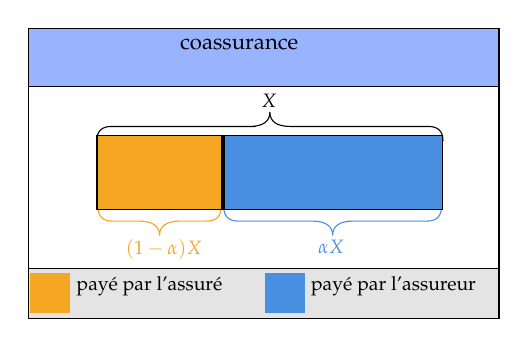
\begin{tikzpicture}[x=0.75pt,y=0.75pt,yscale=-1,xscale=1]
%uncomment if require: \path (0,217); %set diagram left start at 0, and has height of 217

%Shape: Rectangle [id:dp857212648137277] 
\draw  [fill={rgb, 255:red, 255; green, 255; blue, 255 }  ,fill opacity=1 ] (291,53.67) -- (517.8,53.67) -- (517.8,190) -- (291,190) -- cycle ;
%Shape: Rectangle [id:dp6577506986994079] 
\draw  [fill={rgb, 255:red, 228; green, 228; blue, 228 }  ,fill opacity=1 ] (291,169.41) -- (517.8,169.41) -- (517.8,193.67) -- (291,193.67) -- cycle ;
%Shape: Rectangle [id:dp10763459705704914] 
\draw  [fill={rgb, 255:red, 152; green, 180; blue, 255 }  ,fill opacity=1 ] (291,81.92) -- (517.8,81.92) -- (517.8,53.92) -- (291,53.92) -- cycle ;
%Shape: Rectangle [id:dp5604169395708387] 
\draw  [draw opacity=0][fill={rgb, 255:red, 245; green, 166; blue, 35 }  ,fill opacity=1 ] (292,171.41) -- (311.05,171.41) -- (311.05,191.08) -- (292,191.08) -- cycle ;
%Shape: Rectangle [id:dp8289199602562443] 
\draw  [draw opacity=0][fill={rgb, 255:red, 74; green, 144; blue, 226 }  ,fill opacity=1 ] (405.27,171.41) -- (424.32,171.41) -- (424.32,191.08) -- (405.27,191.08) -- cycle ;
%Shape: Brace [id:dp47861464036696866] 
\draw  [color={rgb, 255:red, 245; green, 166; blue, 35 }  ,draw opacity=1 ] (324.54,139.59) .. controls (324.54,144.26) and (326.87,146.59) .. (331.54,146.59) -- (344.24,146.59) .. controls (350.91,146.59) and (354.24,148.92) .. (354.24,153.59) .. controls (354.24,148.92) and (357.57,146.59) .. (364.24,146.59)(361.24,146.59) -- (376.94,146.59) .. controls (381.61,146.59) and (383.94,144.26) .. (383.94,139.59) ;
%Shape: Brace [id:dp08336874707524533] 
\draw  [color={rgb, 255:red, 74; green, 144; blue, 226 }  ,draw opacity=1 ] (385.2,139.59) .. controls (385.2,144.26) and (387.53,146.59) .. (392.2,146.59) -- (427.65,146.59) .. controls (434.32,146.59) and (437.65,148.92) .. (437.65,153.59) .. controls (437.65,148.92) and (440.98,146.59) .. (447.65,146.59)(444.65,146.59) -- (483.09,146.59) .. controls (487.76,146.59) and (490.09,144.26) .. (490.09,139.59) ;
%Shape: Rectangle [id:dp44830624755942683] 
\draw  [draw opacity=0][fill={rgb, 255:red, 74; green, 144; blue, 226 }  ,fill opacity=1 ] (384.8,105.33) -- (490.65,105.33) -- (490.65,140.85) -- (384.8,140.85) -- cycle ;
%Shape: Rectangle [id:dp597465273982372] 
\draw  [draw opacity=0][fill={rgb, 255:red, 245; green, 166; blue, 35 }  ,fill opacity=1 ] (324.15,105.33) -- (384.8,105.33) -- (384.8,140.85) -- (324.15,140.85) -- cycle ;
%Shape: Rectangle [id:dp062060105534497145] 
\draw   (324.15,105.33) -- (490.65,105.33) -- (490.65,140.85) -- (324.15,140.85) -- cycle ;
%Straight Lines [id:da8476063385253465] 
\draw [line width=1.5]    (384.8,105.33) -- (384.8,140.85) ;

%Shape: Brace [id:dp09659689837862229] 
\draw   (490.83,108) .. controls (490.83,103.33) and (488.5,101) .. (483.83,101) -- (417.42,101) .. controls (410.75,101) and (407.42,98.67) .. (407.42,94) .. controls (407.42,98.67) and (404.09,101) .. (397.42,101)(400.42,101) -- (331,101) .. controls (326.33,101) and (324,103.33) .. (324,108) ;

% Text Node
\draw (362.9,57.42) node [anchor=north west][inner sep=0.75pt]  [font=\large] [align=left] {{\footnotesize coassurance}};
% Text Node
\draw (313.05,171.81) node [anchor=north west][inner sep=0.75pt]   [align=left] {{\scriptsize payé par l'assuré}};
% Text Node
\draw (426.02,171.81) node [anchor=north west][inner sep=0.75pt]   [align=left] {{\scriptsize payé par l'assureur}};
% Text Node
\draw (429.36,154.31) node [anchor=north west][inner sep=0.75pt]  [font=\scriptsize] [align=left] {$\displaystyle \textcolor[rgb]{0.29,0.56,0.89}{\alpha X}$};
% Text Node
\draw (336.74,154.31) node [anchor=north west][inner sep=0.75pt]  [font=\scriptsize] [align=left] {$\displaystyle \textcolor[rgb]{0.96,0.65,0.14}{( 1-\alpha ) X}$};
% Text Node
\draw (402,84) node [anchor=north west][inner sep=0.75pt]  [font=\scriptsize] [align=left] {$\displaystyle X$};
\end{tikzpicture}
\end{center}
\end{definitionNOHFILL}

\begin{definitionNOHFILLsub}[L'espérance du montant de perte avec coassurance]
\textbf{L'espérance du montant de perte}, pour l'assureur, \textbf{avec une coassurance de $\alpha$} est \lfbox[formula]{$\text{E}[\alpha X]	=	\alpha \text{E}[X]$}.
\end{definitionNOHFILLsub}


\subsection{Combinaison des facteurs}
\textbf{Cas d'un déductible et de coassurance}
\begin{itemize}
	\item	Habituellement, la coassurance est appliquée \textit{\textbf{après}} le déductible et la perte pour l'assureur est :
		\begin{align*}
		Y^{L}
		&=	\begin{cases}
			0,	&	X \leq d	\\
			\alpha(X - d),	&	X > d
			\end{cases}	\\
		\text{E}[Y^{L}]	
		&=	\alpha\left(\text{E}[X]	-	\text{E}[X \wedge d]	\right)
		\end{align*}
	\item	Si une question spécifie que la coassurance s'applique \textit{\textbf{\textcolor{teal}{avant}}} le déductible, il suffit de remplacer $d$ par $\textcolor{teal}{\frac{d}{\alpha}}$ et mettre le $\alpha$ en évidence comme avant :
		\begin{align*}
		Y^{L}
		&=	\begin{cases}
			0,	&	\alpha X \leq d	\\
			\alpha X - d,	&	\alpha X > d
			\end{cases}	
		=	\begin{cases}
			0,	&	X \leq \textcolor{teal}{\frac{d}{\alpha}}	\\
			\alpha\left(X - \textcolor{teal}{\frac{d}{\alpha}}\right),	&	X > \textcolor{teal}{\frac{d}{\alpha}}
			\end{cases}	\\
		\text{E}[Y^{L}]	
		&=	\alpha\left(\text{E}[X]	-	\text{E}\left[X \wedge \textcolor{teal}{\frac{d}{\alpha}}\right]	\right)
		\end{align*}
\end{itemize}

Soit une police ayant : 
\begin{enumerate}
	\item	une coassurance de $\alpha$,
	\item	une limite de police de $u$,
	\item	un déductible \textit{\textbf{ordinaire}} de $d$.
\end{enumerate}

Alors, \lfbox[formula]{$\text{E}[Y^{L}]	=	\alpha \left\{\text{E}[X \wedge m]	-	\text{E}[X \wedge d]\right\}$} et 
\begin{align*}
	Y^{L}
	&=	\begin{cases}
		0, 	&	X \leq d	\\
		\alpha (X - d), 	&	d < X < m	\\
		u, 	&	X \geq m	
		\end{cases}
\end{align*}
où $m$ est la \textbf{perte maximale admissible}.

\begin{definitionNOHFILLprop}[Perte maximale admissible $m$]
Soit la perte maximale admissible \lfbox[formula]{$m	=	\frac{u}{\alpha} + d$} représentant la plus petite perte pour laquelle l'assureur paye la limite $u$.

\begin{itemize}
	\item	En anglais, \og \textit{maximum covered loss} \fg{}.
\end{itemize}
\end{definitionNOHFILLprop}

Visuellement : 
\begin{center}
\tikzset{every picture/.style={line width=0.75pt}} %set default line width to 0.75pt        
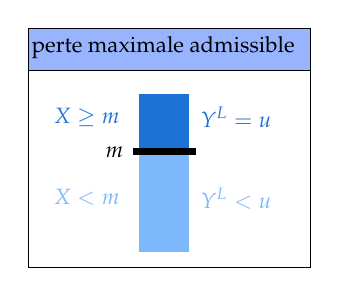
\begin{tikzpicture}[x=0.75pt,y=0.75pt,yscale=-1,xscale=1]
%uncomment if require: \path (0,155); %set diagram left start at 0, and has height of 155

%Shape: Rectangle [id:dp6067733498652601] 
\draw  [fill={rgb, 255:red, 255; green, 255; blue, 255 }  ,fill opacity=1 ] (100.5,13.18) -- (236.5,13.18) -- (236.5,128.67) -- (100.5,128.67) -- cycle ;
%Shape: Rectangle [id:dp4508485722610478] 
\draw  [draw opacity=0][fill={rgb, 255:red, 125; green, 183; blue, 252 }  ,fill opacity=1 ] (178.19,72.58) -- (178.19,121.06) -- (153.95,121.06) -- (153.95,72.58) -- cycle ;
%Shape: Rectangle [id:dp9575111659319537] 
\draw  [draw opacity=0][fill={rgb, 255:red, 29; green, 114; blue, 213 }  ,fill opacity=1 ] (178.19,44.81) -- (178.19,72.58) -- (153.95,72.58) -- (153.95,44.81) -- cycle ;
%Straight Lines [id:da9142966775592043] 
\draw [color={rgb, 255:red, 0; green, 0; blue, 0 }  ,draw opacity=1 ][line width=2.25]    (181.19,72.58) -- (150.99,72.58) ;

%Shape: Rectangle [id:dp3490985301668257] 
\draw  [fill={rgb, 255:red, 152; green, 180; blue, 255 }  ,fill opacity=1 ] (100.5,13.18) -- (236.5,13.18) -- (236.5,33.69) -- (100.5,33.69) -- cycle ;

% Text Node
\draw (101,15.93) node [anchor=north west][inner sep=0.75pt]  [font=\small] [align=left] {{\footnotesize perte maximale admissible}};
% Text Node
\draw (136.5,69.01) node [anchor=north west][inner sep=0.75pt]  [font=\footnotesize] [align=left] {$\displaystyle m$};
% Text Node
\draw (182.5,89.01) node [anchor=north west][inner sep=0.75pt]  [font=\footnotesize,color={rgb, 255:red, 125; green, 183; blue, 252 }  ,opacity=1 ] [align=left] {$\displaystyle Y^{L} < u$};
% Text Node
\draw (182.5,50.01) node [anchor=north west][inner sep=0.75pt]  [font=\footnotesize,color={rgb, 255:red, 29; green, 114; blue, 213 }  ,opacity=1 ] [align=left] {$\displaystyle Y^{L} =u$};
% Text Node
\draw (111.5,89.51) node [anchor=north west][inner sep=0.75pt]  [font=\footnotesize,color={rgb, 255:red, 125; green, 183; blue, 252 }  ,opacity=1 ] [align=left] {$\displaystyle X< m$};
% Text Node
\draw (111.5,50.51) node [anchor=north west][inner sep=0.75pt]  [font=\footnotesize,color={rgb, 255:red, 29; green, 114; blue, 213 }  ,opacity=1 ] [align=left] {$\displaystyle X\geq m$};
\end{tikzpicture}
\end{center}

%\begin{align*}
%Y^{(L\textcolor{blue}{|P)}}_{(O)} 
%	&=	\begin{cases}
%			(0 {\color{blue}{| \text{Non-défini})}},	&	\ x  < \frac{d}{1 + r} \\
%			\alpha \Big((1 + r) x - d \Big),	&	\ \frac{d}{1 + r} \leq x < \frac{u}{1 + r} \\
%			\alpha (u - d),	&	\ x \geq \frac{u}{1 + r} \\
%		\end{cases}	\\
%	\esp{Y^{(L\textcolor{blue}{|P)}}_{(O)}} 
%	&=	\frac{\alpha (1 + r) \left( 
%			\text{E}\left[X \wedge \frac{u}{1 + r}\right] -  
%			\text{E}\left[X \wedge \frac{d}{1 + r}\right]  
%		\right)}{{\color{blue}{S_{X} \left(\frac{d}{1 + r}\right)}}} 
%\end{align*}


\columnbreak
\subsection{Inflation}
\begin{definitionNOHFILL}[Inflation $r$]
L'inflation de \lfbox[formula]{$r$} augmente les coûts mais, de façon générale, ils sont couverts par la compagnie d'assurance et ne cause pas de changements à la police.
\end{definitionNOHFILL}

\begin{definitionNOHFILLsub}[L'espérance du montant de perte avec inflation]
\textbf{L'espérance du montant de perte}, pour l'assureur, \textbf{avec de l'inflation de $r$} est \lfbox[formula]{$\text{E}[(1 + r) X]	=	(1 + r) \text{E}[X]$}.\\

Combiné avec les autres facteurs :

\begin{align*}
	\text{E}\left[Y^{L}\right]		
	&=	\alpha(1 + r) \left(\text{E}\left[X \wedge \frac{m}{1 + r}\right]	-	\text{E}\left[X \wedge \frac{d}{1 + r}\right]\right)	\\
	\text{E}\left[Y^{P}\right]	
	&=	\frac{\text{E}[Y^{L}]}{S_{X}\left(\frac{d}{1 + r}\right)}
\end{align*}
\end{definitionNOHFILLsub}

\paragraph{Note}	Si la distribution de $X$ comporte un paramètre d'échelle $\theta$, on peut simplifier les équations en posant \lfbox[formula]{$\theta'	=	(1 + r)\theta$}.



\pagebreak
\section{Estimation de modèles non paramétriques}
\subsection{Données complètes}
\hl{Section à compléter avec mes notes de IARD et 11.2 de Nonlife Actuariel Models (tse).}
\subsubsection{Distribution empirique}
\begin{definitionNOHFILL}[Distribution empirique]
Distribution discrète prenant comme valeurs $y_{1}, \dots, y_{m}$ avec probabilités $\frac{w_{1}}{n}, \dots, \frac{w_{m}}{n}$;
\begin{itemize}
	\item	On peut également la définir comme la distribution discrète équiprobable des valeurs $x_{1}, \dots, x_{n}$.
\end{itemize}
\end{definitionNOHFILL}

\begin{distributions}[Notation]
\begin{description}
	\item[$\hat{f}()$]	Fonction de densité empirique.	
	\item[$\hat{F}()$]	Fonction de répartition empirique.	
	\item[$\tilde{F}()$]	Fonction de répartition lissée;
		\begin{itemize}
		\item	En anglais, \og \textit{smoothed empirical distribution function} \fg{}.
		\item	On appel parfois la fonction de répartition \textit{la fonction distribution} (\og \textit{distribution function} \fg{}).
		\end{itemize}
%	\item[Moyenne de la distribution empirique]
%		\begin{align*}
%		\sumz{m}{j = 1} \frac{w_{j}}{n} y_{j}
%		&=	\frac{1}{n} \sumz{n}{i = 1} x_{i}
%		\end{align*}
%	\item[Variance de la distribution empirique]
%		\begin{align*}
%		\sumz{m}{j = 1} \frac{w_{j}}{n} (y_{j} - \bar{x})^{2}
%		&=	\frac{1}{n} \sumz{n}{i = 1} (y_{i} - \bar{x})^{2}
%		\end{align*}
\end{description}
\end{distributions}

\begin{align*}
	\hat{f}(y)
	&=	\begin{cases}
		\frac{w_{j}}{n},	&	\text{si } y = y_{j} \, \forall j	\\
		0,	\text{sinon}
		\end{cases}	\\
		\hat{F}(y)
	&=	\begin{cases}
		0,	&	y	<	y_{1},	\\
		\frac{1}{n}\sumz{j}{h = 1}w_{h},	&	y_{j}	\leq	y	<	y_{j + 1}, \, j	=	1, \dots, m - 1	\\
		1,	&	y_{m}	\leq	y
		\end{cases}
\end{align*}		

On peut estimer la valeur de $\hat{F}()$ pour un une valeur de $y$ pas dans l'ensemble $y_{1}, \dots, y_{m}$ avec la fonction de répartition lissée $\tilde{F}()$. Pour \icbox[red][palechestnut]{$y_{j} \leq y < y_{j + 1}$} et \icbox[red][palechestnut]{$j \in \{1, 2, \dots, m - 1\}$}, $\tilde{F}(y)$ est une interpolation linéaire de $\hat{F}(y_{j + 1})$ et $\hat{F}(y_{j})$ :
\begin{align*}
	\tilde{F}(y)
	&=	\frac{y	-	y_{j	}}{y_{j + 1}	-	y_{j}}\hat{F}(y_{j + 1})  + 
		\frac{y_{j + 1}	-	y_{j	}}{y_{j + 1}	-	y_{j}}\hat{F}(y_{j})
\end{align*}

\begin{definitionNOHFILLprop}[Distribution Binomiale de la fonction de répartition empirique]
On peut écrire la fonction de répartition empirique comme \lfbox[formula]{$\hat{F}(y)	=	\frac{Y}{n}$} où $Y$ est le nombre d'observations qui sont inférieures ou égales à $y$ tel que \lfbox[formula]{$Y \sim \text{Bin}(n, p = F(y))$}.\\

On trouve :
\begin{align*}
	\text{E}[Y]	
	&=	\frac{\text{E}[\hat{F}(y)]}{n}
	=	F(y)		\\
	\text{Var}(Y)
	&=	\frac{\text{Var}(\hat{F}(y))}{n^{2}}
	=	\frac{F(y)(1 - F(y))}{n}
\end{align*}
\end{definitionNOHFILLprop}


\subsubsection{Estimation par noyaux}
La fonction de répartition empirique résume les données d'une distribution discrète. Cependant, lorsque la variable d'intérêt $X$ est continue on souhaite estimer une fonction de densité.

Pour une observation $x_{i}$ de l'échantillon, la fonction de répartition empirique assigne une masse de probabilité de $1/n$ au point $x_{i}$.
Puisque $X$ est continue, il est normal que l'on souhaite \underline{\textit{distribuer}} cette masse \textit{autour} de $x_{i}$.

Si l'on souhaite distribuer cette masse de façon égale, on le fait sur l'intervalle \icbox{$[x_{i}  - b, x_{i} + b]$} avec la fonction de $x_{i}$ $f_{i}(x)$:
\begin{align*}
	f_{i}(x)
	&=	\begin{cases}
		\frac{0.5}{b},	&	x_{i} - b	\leq		x	\leq		x_{i} + b,	\\
		0,	&	\text{sinon}
		\end{cases}	
\end{align*}
\begin{itemize}[leftmargin = *]
	\item	Cette fonction est rectangulaire avec une base de longueur $2b$ et une hauteur de $0.5/b$ pour avoir une aire de 1.
	\item	On peut l'interpréter comme la fonction de densité contribué par l'observation $x_{i}$;
	\item	On note que ceci correspond à la fonction de densité d'une distribution uniforme $U(x_{i} -  b, x_{i} + b)$;
	\item	Alors, seulement les valeurs de $x$ contenues dans l'intervalle $(x_{i} -  b, x_{i} + b)$ reçoivent une "contribution" de $x_{i}$;
	\item	La fonction de densité de $X$ est donc la somme des masses de probabilité contribuées \icbox[red][palechestnut]{$\tilde{f}(x)	=	\frac{1}{n} \sumz{n}{i = 1}(x)$}.
\end{itemize}

On défini $\phi_{i}	=	\frac{x - x_{i}}{b}$ et $K_{R}(\phi)$:
\begin{align*}
	K_{R}(\phi)
	&=	\begin{cases}
		\frac{1}{2},	&	-1	\leq		\phi	\leq		1,	\\
		0,	&	\text{sinon}
		\end{cases}	
\end{align*}
\begin{itemize}[leftmargin = *]
	\item	On trouve donc que \icbox[red][palechestnut]{$f_{i}(x)	=	\frac{1}{b}K_{R}(\phi_{i})$} et \icbox[red][palechestnut]{$\tilde{f}(x)	=	\frac{1}{nb}\sumz{n}{i = 1}K_{R}(\phi_{i})$}.
\end{itemize}

\begin{distributions}[Notation]
\begin{description}
	\item[$b$]	\og \textit{bandwith} \fg{} où \icbox[red][palechestnut]{$b > 0$};
	\item[$K_{R}(\phi)$]	\og \textit{rectangular (box, uniform) kernel function} \fg{};
	\item[$\tilde{f}(x)$]	Estimation de la fonction de densité selon le noyaux rectangulaire;
	\item[$K_{T}(\phi)$]	\og \textit{triangular kernel} \fg{};
	\begin{align*}
		K_{R}(\phi)
		&=	\begin{cases}
			1 - |\phi|,	&	-1	\leq		\phi	\leq		1,	\\
			0,	&	\text{sinon}
			\end{cases}	
	\end{align*}
	\item[$K_{G}(\phi)$]	\og \textit{Gaussian kernel} \fg{};
		\begin{align*}
		K_{G}(\phi)
		&=	\frac{1}{\sqrt{2\pi}} \textrm{e}^{-\frac{\phi^{2}}{2}}, -\infty	<	\phi	<	\infty
		\end{align*}
\end{description}
\end{distributions}




\columnbreak
\subsection{Données incomplètes}
\hl{Section à compléter avec mes notes de IARD et 11.2 de Nonlife Actuariel Models (tse).}
\subsubsection{Estimateur de Kaplan-Meier}
Soit : 
\begin{align*}
	S(y_{j})
	&=	\Pr(X > y_{1})	\Pr(X > y_{2} | X > y_{1}) \hdots \Pr(X > y_{j} | X > y_{j - 1})
	=	\Pr(X > y_{1}) \prod_{h = 2}^{j} \Pr(X > y_{h} | X > y_{h - 1})
\end{align*}

Où on peut estimer $\widehat{\Pr}(X > y_{1})	=	1	-	\frac{w_{1}}{r_{1}}$ et $\widehat{\Pr}(X > y_{h} | X > y_{h - 1})	=	1	-	\frac{w_{h}}{r_{h}}$ pour \lfbox[conditions]{$h	=	2, \dots, m$}.

Il s'ensuit qu'on peut estimer $S(y_{j})$ par :
\begin{align*}
	\hat{S}(y_{j})
	&=	\prod_{h = 1}^{j} \left(1 - \frac{w_{h}}{r_{h}}\right)
\end{align*}

Variance de l'estimateur Kaplan-Meier : \lfbox[formula]{$\text{Var}(\hat{S}_{K}(y_{j}) | \mathcal{C})	\approx	\left(S(y_{j})\right)^{2} \left(\sum^{j}_{h = 1} \frac{1 - S_{h}}{S_{h}r_{h}}\right)$} 
Approximation de Greenwood de la variance de l'estimateur Kaplan-Meier : \lfbox[formula]{$\widehat{\text{Var}}(\hat{S}_{K}(y_{j}) | \mathcal{C})	\approx	\left(\hat{S}_{K}(y_{j})\right)^{2} \left(\sum^{j}_{h = 1} \frac{w_{h}}{r_{h} (r_{h} - w_{h})}\right)$} 


\subsubsection{Estimateur de Nelson-Aalen}
\begin{distributions}[Notation]
\begin{description}
	\item[$h(y)$]	Fonction de hasard.
	\item[$H(y)$]	Fonction de hasard cumulative.
\end{description}
\end{distributions} 

\begin{align*}
	H(y)
	&=	\int_{0}^{y} h(y) dy
\end{align*}

Il s'ensuit que \lfbox[formula]{$S(y)	=	\textrm{e}^{-H(y)}$} et \lfbox[formula]{$H(y)	=	-\ln\left(S(y)\right)$}.

Avec l'approximation \lfbox[conditions]{$-\ln\left(1	-	\frac{w_{h}}{r_{h}}\right)	\approx	\frac{w_{h}}{r_{h}}$} on trouve que \lfbox[formula]{$H(y)	=	\sum_{h	=	1}^{j} \frac{w_{h}}{r_{h}}$} qui correspond à l'\textbf{estimateur Nelson-Aalen} de la fonction de hasard cumulative.

\columnbreak
\subsection{Données groupées}
\hl{Section à compléter avec mes notes de IARD et 11.3 de Nonlife Actuariel Models (tse).}



\pagebreak
\section{Estimation de modèles paramétriques}
\subsection*{Estimation par maximum de vraisemblance pour des données incomplètes et groupées}
Lorsque les données sont groupées et/ou incomplètes, les observations ne sont plus iid mais on peut quand même formuler la fonction de vraisemblance et trouver l'EMV.

La première étape est d'écrire la fonction de (log) vraisemblance adéquate pour la méthode d'échantillonnage des données.\\

Par exemple, soit des données groupées en $k$ intervalles : 
\begin{itemize}
	\item	On trouve avec la fonction de répartition $F(\cdot; \theta)$ que la probabilité d'être dans l'intervalle $(c_{j - 1}, c_{j}]$ est $F(c_{j}; \theta)	-	F(c_{j - 1}; \theta)$;
	\item	On pose que les observations individuelles sont iid;
	\item	Donc, la vraisemblance d'avoir $n_{j}$ observations dans l'intervalle $(c_{j - 1}, c_{j}]$, \lfbox[conditions]{pour $j	=	1, \dots, k$ et $\bm{n}	=	(n_{1}, \cdots, n_{k})$} est :
		\begin{align*}
		\mathcal{L}(\theta; \bm{n})
		&=	\prod^{k}_{j	=	1} \left[F(c_{j}; \theta)	-	F(c_{j - 1}; \theta)\right]^{n_{j}}
		\end{align*}
\end{itemize}


\setlength{\mathindent}{-0.75cm}
\begin{algo}{Fonction de vraisemblance}
\begin{align*}
	\mathcal{L}(\theta; \bm{x})
	&=	\prod^{k}_{j	=	1} \underbrace{f(x_{j}; \theta)}_{\shortstack{probabilité de chaque\\ observation à la\\ valeur observée}}	&
	\shortstack{données complètes}	
\end{align*}

\tcbline

Données groupées en $k$ intervalles:\\
\begin{align*}
	\mathcal{L}(\theta; \bm{n})
	&=	\prod^{k}_{j	=	1} \underbrace{\left[F(c_{j}; \theta)	-	F(c_{j - 1}; \theta)\right]^{n_{j}}}_{\shortstack{probabilité d'une\\ observation dans\\ l'intervalle}}		&
	\shortstack{données groupées}	
\end{align*}

\tcbline

Données censurées vers la droite avec $n_{1}$ observations complètes et $n_{2}$ observations censurées à la limite de $u$:\\
\begin{align*}
	\mathcal{L}(\theta; \bm{x}, n_{2})
	&=	\underbrace{\left[\prod^{n_{1}}_{i	=	1} f(x_{i}; \theta) \right]}_{\shortstack{probabilité de chaque\\ observation à la\\ valeur observée}} \overbrace{\left[1	-	F(u; \theta)\right]^{n_{2}}}^{\shortstack{probabilité qu'une\\ observation soit\\ d'au moins $u$}}		&
	\shortstack{données censurées\\ vers la droite}	\\
\end{align*}

\tcbline

Données tronquées vers la gauche avec un déductible de $d$:\\
\begin{align*}
	\mathcal{L}(\theta; \bm{x})
	&=	\underbrace{\frac{1}{\left[1	-	F(d; \theta)\right]^{n}}}_{\shortstack{pondère par la\\ probabilité d'être\\ supérieur au déductible}} \prod^{n}_{i	=	1} f(x_{i}; \theta)	&
	\shortstack{données censurées\\ vers la droite}	\\
\end{align*}
\end{algo}
\setlength{\mathindent}{1cm}



\pagebreak
\section{Évaluation et sélection de modèles}
\hl{Cette section n'est pas suffisamment bien expliquée pour que je la considère complète.}\\
\begin{rappel_enhanced}[Contexte]
Évaluer les modèles avec des méthodes non paramétriques a l'avantage d'avoir très peu d'hypothèses. Cependant, il est plus difficile d'évaluer le modèle d'un point de vue théorique.

Évaluer les modèles avec des méthodes paramétriques a l'avantage de résumer le modèle à un petit nombre de paramètres. Cependant, ces méthodes sont une simplification et risquent d'imposer la mauvaise structure.
\end{rappel_enhanced}

\subsection{Graphiquement}
Avec les méthodes d'évaluation visuelles, on peut détecter si les données diffèrent anormalement du modèle paramétrique.
\begin{itemize}
	\item	On peut évaluer la fonction de répartition empirique et la fonction de répartition théorique sur un même graphique pour évaluer l'ajustement.
	\item	On peut évaluer le tracé des probabilités (\og \textit{P-P plot} \fg{}) qui trace la répartition empirique et la répartition théorique.
	\item	On peut tracer l'histogramme des données et superposer la densité théorique pour évaluer l'ajustement.
\end{itemize}

Le désavantage de ces méthodes est qu'elle ne fournissent pas des mesures quantitatives sur l'ajustement du modèle.


\subsection{Tests pour la qualité de l'ajustement}
\begin{definitionNOHFILL}[Tests de spécification (\og \textit{misspecification tests} \fg{})]
Test de signifiance dont l'objectif est d'évaluer les hypothèses de distribution d'un modèle.

\end{definitionNOHFILL}

\begin{distributions}[Notation]
\begin{description}
	\item[$F^{\ast}()$]	Fonction de répartition d'une v.a. continue (hypothèse nulle).
	\item[$\hat{F}()$]	Fonction de répartition empirique.
\end{description}
\end{distributions}

Les tests de Kolmogorov-Smirnov (K.-S.) et de Anderson-Darling sont idéales lorsque l'on désire comparer les fonctions de répartition. \\

Le test de K.-S. compare la fonction de distribution (répartition) empirique à celle d'une distribution théorique. L'idée du test est donc de quantifier l'évaluation visuelle que l'on peut faire de l'ajustement.

\begin{definitionNOHFILLsub}[Test de Kolmogorov-Smirnov]
On teste si les données semblent suivre une distribution (« supportent l'hypothèse nulle ») avec la statistique de Kolmogorov-Smirnov : \lfbox[formula]{$D	=	\underset{x_{(1)}	\leq	x	\leq	x_{(n)}}{\max} \left| \hat{F}(x)	-	F^{\ast}(x) \right|$}.
\begin{itemize}
	\item	Ceci équivaut donc à calculer la différence maximale entre la fonction de répartition empirique et celle de la distribution.
	\item	Puisque $\hat{F}()$ est une fonction à escalier, il faut seulement évaluer la fonction aux points observés $x_{(1)}	\leq	x_{(2)}	\leq	\hdots	\leq	x_{(n)}$.
%%%	------------------------
%%%	NOTES
%%%	+	why?
%%%	------------------------
	\item	De plus, le maximum peut seulement arriver soit au point de saut $x_{(i)}$ ou immédiatement avant $x_{(i - 1)}$.
\end{itemize}

On peut donc récrire\\ \lfbox[formula]{$D	=	\underset{i \in \{1, \dots, n\}}{\max}\left\{ \max\left\{\left| \hat{F}(x_{(i - 1)})	-	F^{\ast}(x_{(i)}) \right|, \left| \hat{F}(x_{(i)})	-	F^{\ast}(x_{(i)}) \right|\right\}\right\}$}.

\begin{itemize}
	\item	Si les données sont bien ajustées, on s'attend à ce que $D$ soit très petit.
	\item	Lorsque la distribution est entièrement spécifiée (aucun paramètres sont estimés) une table avec les valeurs critiques est donnée.
	\item	S'il faut estimer des paramètres, la simulation Monte-Carlo est utilisée pour trouver des nouvelles valeurs critiques.
\end{itemize}
\end{definitionNOHFILLsub}

\begin{definitionNOHFILLprop}[Test de K.-S. pour des données incomplètes]
Pour des données tronquées à $d$ et censurée (vers la droite) à $u$, \lfbox[formula]{$D	=	\underset{d	\leq	x	\leq	u}{\max} \left| \hat{F}(x)	-	F^{\ast}(x) \right|$}
\end{definitionNOHFILLprop}

Visuellement, le test de K.-S. ressemble à :
\begin{center}
\tikzset{every picture/.style={line width=0.75pt}} %set default line width to 0.75pt        

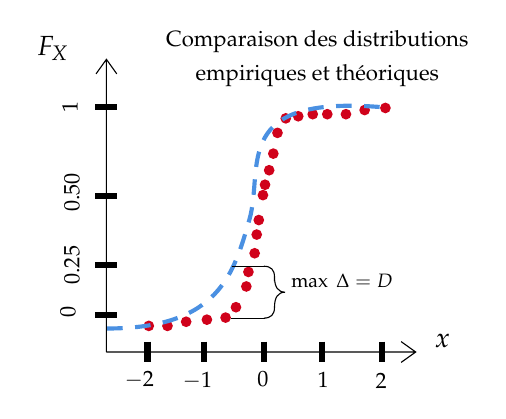
\begin{tikzpicture}[x=0.75pt,y=0.75pt,yscale=-1,xscale=1]
%uncomment if require: \path (0,300); %set diagram left start at 0, and has height of 300

%Shape: Axis 2D [id:dp24483060574985016] 
\draw  (159.17,162) -- (308.17,162)(159.17,21) -- (159.17,162) -- cycle (301.17,157) -- (308.17,162) -- (301.17,167) (154.17,28) -- (159.17,21) -- (164.17,28)  ;
%Straight Lines [id:da6030801017105296] 
\draw [line width=2.25]    (179,157) -- (179,167) ;
%Straight Lines [id:da2652234915508369] 
\draw [line width=2.25]    (206,157) -- (206,167) ;
%Straight Lines [id:da7718269955671673] 
\draw [line width=2.25]    (235,157) -- (235,167) ;
%Straight Lines [id:da8049939015901117] 
\draw [line width=2.25]    (263,157) -- (263,167) ;
%Straight Lines [id:da5692977431446764] 
\draw [line width=2.25]    (292,157) -- (292,167) ;
%Straight Lines [id:da036135237157260525] 
\draw [line width=2.25]    (153.67,44) -- (164.5,44) ;
%Straight Lines [id:da021466328536539292] 
\draw [line width=2.25]    (153.67,87) -- (164.5,87) ;
%Straight Lines [id:da8388615672035813] 
\draw [line width=2.25]    (153.67,120) -- (164.5,120) ;
%Straight Lines [id:da4377316999274832] 
\draw [line width=2.25]    (153.67,144) -- (164.5,144) ;
%Flowchart: Connector [id:dp27902589825476154] 
\draw  [draw opacity=0][fill={rgb, 255:red, 208; green, 2; blue, 27 }  ,fill opacity=1 ] (186,149.42) .. controls (186,147.99) and (187.16,146.83) .. (188.58,146.83) .. controls (190.01,146.83) and (191.17,147.99) .. (191.17,149.42) .. controls (191.17,150.84) and (190.01,152) .. (188.58,152) .. controls (187.16,152) and (186,150.84) .. (186,149.42) -- cycle ;
%Flowchart: Connector [id:dp8858881991629384] 
\draw  [draw opacity=0][fill={rgb, 255:red, 208; green, 2; blue, 27 }  ,fill opacity=1 ] (177,149.42) .. controls (177,147.99) and (178.16,146.83) .. (179.58,146.83) .. controls (181.01,146.83) and (182.17,147.99) .. (182.17,149.42) .. controls (182.17,150.84) and (181.01,152) .. (179.58,152) .. controls (178.16,152) and (177,150.84) .. (177,149.42) -- cycle ;
%Flowchart: Connector [id:dp965947428222834] 
\draw  [draw opacity=0][fill={rgb, 255:red, 208; green, 2; blue, 27 }  ,fill opacity=1 ] (195,147.42) .. controls (195,145.99) and (196.16,144.83) .. (197.58,144.83) .. controls (199.01,144.83) and (200.17,145.99) .. (200.17,147.42) .. controls (200.17,148.84) and (199.01,150) .. (197.58,150) .. controls (196.16,150) and (195,148.84) .. (195,147.42) -- cycle ;
%Flowchart: Connector [id:dp5208785016321031] 
\draw  [draw opacity=0][fill={rgb, 255:red, 208; green, 2; blue, 27 }  ,fill opacity=1 ] (205,146.42) .. controls (205,144.99) and (206.16,143.83) .. (207.58,143.83) .. controls (209.01,143.83) and (210.17,144.99) .. (210.17,146.42) .. controls (210.17,147.84) and (209.01,149) .. (207.58,149) .. controls (206.16,149) and (205,147.84) .. (205,146.42) -- cycle ;
%Flowchart: Connector [id:dp2872263470627334] 
\draw  [draw opacity=0][fill={rgb, 255:red, 208; green, 2; blue, 27 }  ,fill opacity=1 ] (214,145.42) .. controls (214,143.99) and (215.16,142.83) .. (216.58,142.83) .. controls (218.01,142.83) and (219.17,143.99) .. (219.17,145.42) .. controls (219.17,146.84) and (218.01,148) .. (216.58,148) .. controls (215.16,148) and (214,146.84) .. (214,145.42) -- cycle ;
%Flowchart: Connector [id:dp6170797725926003] 
\draw  [draw opacity=0][fill={rgb, 255:red, 208; green, 2; blue, 27 }  ,fill opacity=1 ] (219,140.42) .. controls (219,138.99) and (220.16,137.83) .. (221.58,137.83) .. controls (223.01,137.83) and (224.17,138.99) .. (224.17,140.42) .. controls (224.17,141.84) and (223.01,143) .. (221.58,143) .. controls (220.16,143) and (219,141.84) .. (219,140.42) -- cycle ;
%Flowchart: Connector [id:dp6321853947189746] 
\draw  [draw opacity=0][fill={rgb, 255:red, 208; green, 2; blue, 27 }  ,fill opacity=1 ] (224,130.42) .. controls (224,128.99) and (225.16,127.83) .. (226.58,127.83) .. controls (228.01,127.83) and (229.17,128.99) .. (229.17,130.42) .. controls (229.17,131.84) and (228.01,133) .. (226.58,133) .. controls (225.16,133) and (224,131.84) .. (224,130.42) -- cycle ;
%Flowchart: Connector [id:dp4527459516123209] 
\draw  [draw opacity=0][fill={rgb, 255:red, 208; green, 2; blue, 27 }  ,fill opacity=1 ] (225,123.42) .. controls (225,121.99) and (226.16,120.83) .. (227.58,120.83) .. controls (229.01,120.83) and (230.17,121.99) .. (230.17,123.42) .. controls (230.17,124.84) and (229.01,126) .. (227.58,126) .. controls (226.16,126) and (225,124.84) .. (225,123.42) -- cycle ;
%Flowchart: Connector [id:dp5990586632002524] 
\draw  [draw opacity=0][fill={rgb, 255:red, 208; green, 2; blue, 27 }  ,fill opacity=1 ] (228,114.42) .. controls (228,112.99) and (229.16,111.83) .. (230.58,111.83) .. controls (232.01,111.83) and (233.17,112.99) .. (233.17,114.42) .. controls (233.17,115.84) and (232.01,117) .. (230.58,117) .. controls (229.16,117) and (228,115.84) .. (228,114.42) -- cycle ;
%Flowchart: Connector [id:dp46008272444906795] 
\draw  [draw opacity=0][fill={rgb, 255:red, 208; green, 2; blue, 27 }  ,fill opacity=1 ] (229,105.42) .. controls (229,103.99) and (230.16,102.83) .. (231.58,102.83) .. controls (233.01,102.83) and (234.17,103.99) .. (234.17,105.42) .. controls (234.17,106.84) and (233.01,108) .. (231.58,108) .. controls (230.16,108) and (229,106.84) .. (229,105.42) -- cycle ;
%Flowchart: Connector [id:dp10208355949407677] 
\draw  [draw opacity=0][fill={rgb, 255:red, 208; green, 2; blue, 27 }  ,fill opacity=1 ] (243,49.42) .. controls (243,47.99) and (244.16,46.83) .. (245.58,46.83) .. controls (247.01,46.83) and (248.17,47.99) .. (248.17,49.42) .. controls (248.17,50.84) and (247.01,52) .. (245.58,52) .. controls (244.16,52) and (243,50.84) .. (243,49.42) -- cycle ;
%Flowchart: Connector [id:dp44081367516766856] 
\draw  [draw opacity=0][fill={rgb, 255:red, 208; green, 2; blue, 27 }  ,fill opacity=1 ] (249,48.42) .. controls (249,46.99) and (250.16,45.83) .. (251.58,45.83) .. controls (253.01,45.83) and (254.17,46.99) .. (254.17,48.42) .. controls (254.17,49.84) and (253.01,51) .. (251.58,51) .. controls (250.16,51) and (249,49.84) .. (249,48.42) -- cycle ;
%Flowchart: Connector [id:dp258791942489629] 
\draw  [draw opacity=0][fill={rgb, 255:red, 208; green, 2; blue, 27 }  ,fill opacity=1 ] (256,47.42) .. controls (256,45.99) and (257.16,44.83) .. (258.58,44.83) .. controls (260.01,44.83) and (261.17,45.99) .. (261.17,47.42) .. controls (261.17,48.84) and (260.01,50) .. (258.58,50) .. controls (257.16,50) and (256,48.84) .. (256,47.42) -- cycle ;
%Flowchart: Connector [id:dp7461727454132954] 
\draw  [draw opacity=0][fill={rgb, 255:red, 208; green, 2; blue, 27 }  ,fill opacity=1 ] (230,98.42) .. controls (230,96.99) and (231.16,95.83) .. (232.58,95.83) .. controls (234.01,95.83) and (235.17,96.99) .. (235.17,98.42) .. controls (235.17,99.84) and (234.01,101) .. (232.58,101) .. controls (231.16,101) and (230,99.84) .. (230,98.42) -- cycle ;
%Flowchart: Connector [id:dp3590383056585824] 
\draw  [draw opacity=0][fill={rgb, 255:red, 208; green, 2; blue, 27 }  ,fill opacity=1 ] (232,86.42) .. controls (232,84.99) and (233.16,83.83) .. (234.58,83.83) .. controls (236.01,83.83) and (237.17,84.99) .. (237.17,86.42) .. controls (237.17,87.84) and (236.01,89) .. (234.58,89) .. controls (233.16,89) and (232,87.84) .. (232,86.42) -- cycle ;
%Flowchart: Connector [id:dp1884350833419266] 
\draw  [draw opacity=0][fill={rgb, 255:red, 208; green, 2; blue, 27 }  ,fill opacity=1 ] (233,81.42) .. controls (233,79.99) and (234.16,78.83) .. (235.58,78.83) .. controls (237.01,78.83) and (238.17,79.99) .. (238.17,81.42) .. controls (238.17,82.84) and (237.01,84) .. (235.58,84) .. controls (234.16,84) and (233,82.84) .. (233,81.42) -- cycle ;
%Flowchart: Connector [id:dp24880669696449487] 
\draw  [draw opacity=0][fill={rgb, 255:red, 208; green, 2; blue, 27 }  ,fill opacity=1 ] (235,74.42) .. controls (235,72.99) and (236.16,71.83) .. (237.58,71.83) .. controls (239.01,71.83) and (240.17,72.99) .. (240.17,74.42) .. controls (240.17,75.84) and (239.01,77) .. (237.58,77) .. controls (236.16,77) and (235,75.84) .. (235,74.42) -- cycle ;
%Flowchart: Connector [id:dp23618438280038845] 
\draw  [draw opacity=0][fill={rgb, 255:red, 208; green, 2; blue, 27 }  ,fill opacity=1 ] (237,66.42) .. controls (237,64.99) and (238.16,63.83) .. (239.58,63.83) .. controls (241.01,63.83) and (242.17,64.99) .. (242.17,66.42) .. controls (242.17,67.84) and (241.01,69) .. (239.58,69) .. controls (238.16,69) and (237,67.84) .. (237,66.42) -- cycle ;
%Flowchart: Connector [id:dp38788335050603684] 
\draw  [draw opacity=0][fill={rgb, 255:red, 208; green, 2; blue, 27 }  ,fill opacity=1 ] (239,56.42) .. controls (239,54.99) and (240.16,53.83) .. (241.58,53.83) .. controls (243.01,53.83) and (244.17,54.99) .. (244.17,56.42) .. controls (244.17,57.84) and (243.01,59) .. (241.58,59) .. controls (240.16,59) and (239,57.84) .. (239,56.42) -- cycle ;
%Flowchart: Connector [id:dp8001516680880116] 
\draw  [draw opacity=0][fill={rgb, 255:red, 208; green, 2; blue, 27 }  ,fill opacity=1 ] (272,47.42) .. controls (272,45.99) and (273.16,44.83) .. (274.58,44.83) .. controls (276.01,44.83) and (277.17,45.99) .. (277.17,47.42) .. controls (277.17,48.84) and (276.01,50) .. (274.58,50) .. controls (273.16,50) and (272,48.84) .. (272,47.42) -- cycle ;
%Flowchart: Connector [id:dp06230967753042438] 
\draw  [draw opacity=0][fill={rgb, 255:red, 208; green, 2; blue, 27 }  ,fill opacity=1 ] (263,47.42) .. controls (263,45.99) and (264.16,44.83) .. (265.58,44.83) .. controls (267.01,44.83) and (268.17,45.99) .. (268.17,47.42) .. controls (268.17,48.84) and (267.01,50) .. (265.58,50) .. controls (264.16,50) and (263,48.84) .. (263,47.42) -- cycle ;
%Flowchart: Connector [id:dp4843810494735361] 
\draw  [draw opacity=0][fill={rgb, 255:red, 208; green, 2; blue, 27 }  ,fill opacity=1 ] (281,45.42) .. controls (281,43.99) and (282.16,42.83) .. (283.58,42.83) .. controls (285.01,42.83) and (286.17,43.99) .. (286.17,45.42) .. controls (286.17,46.84) and (285.01,48) .. (283.58,48) .. controls (282.16,48) and (281,46.84) .. (281,45.42) -- cycle ;
%Flowchart: Connector [id:dp9279424690148039] 
\draw  [draw opacity=0][fill={rgb, 255:red, 208; green, 2; blue, 27 }  ,fill opacity=1 ] (291,44.42) .. controls (291,42.99) and (292.16,41.83) .. (293.58,41.83) .. controls (295.01,41.83) and (296.17,42.99) .. (296.17,44.42) .. controls (296.17,45.84) and (295.01,47) .. (293.58,47) .. controls (292.16,47) and (291,45.84) .. (291,44.42) -- cycle ;
%Curve Lines [id:da002395199379529034] 
\draw [color={rgb, 255:red, 74; green, 144; blue, 226 }  ,draw opacity=1 ][line width=1.5]  [dash pattern={on 5.63pt off 4.5pt}]  (159.5,150.67) .. controls (213.5,150.67) and (220.5,124.17) .. (228,98.42) .. controls (235.5,72.67) and (217.5,36.67) .. (296.17,44.42) ;
%Shape: Brace [id:dp6799486612215031] 
\draw   (235,145.67) .. controls (238.43,145.67) and (240.15,143.95) .. (240.15,140.52) -- (240.15,140.52) .. controls (240.15,135.62) and (241.86,133.17) .. (245.29,133.17) .. controls (241.86,133.17) and (240.15,130.72) .. (240.15,125.81)(240.15,128.02) -- (240.15,125.81) .. controls (240.15,122.38) and (238.43,120.67) .. (235,120.67) ;
%Straight Lines [id:da08941638414935005] 
\draw    (219.5,120.67) -- (235.5,120.67) ;
%Straight Lines [id:da34946556635800796] 
\draw    (219.17,145.67) -- (235.5,145.67) ;

% Text Node
\draw (183,6) node [anchor=north west][inner sep=0.75pt]   [align=left] {\begin{minipage}[lt]{114.75000000000001pt}\setlength\topsep{0pt}
\begin{center}
{\footnotesize Comparaison des distributions }\\{\footnotesize empiriques et théoriques }
\end{center}

\end{minipage}};
% Text Node
\draw (314,152) node [anchor=north west][inner sep=0.75pt]   [align=left] {\begin{minipage}[lt]{8.67pt}\setlength\topsep{0pt}
\begin{center}
$\displaystyle x$
\end{center}

\end{minipage}};
% Text Node
\draw (121.5,8.5) node [anchor=north west][inner sep=0.75pt]   [align=left] {\begin{minipage}[lt]{16.001216pt}\setlength\topsep{0pt}
\begin{center}
$\displaystyle F_{X}$
\end{center}

\end{minipage}};
% Text Node
\draw (166.62,170.3) node [anchor=north west][inner sep=0.75pt]  [font=\footnotesize] [align=left] {$\displaystyle -2$};
% Text Node
\draw (194.62,170.3) node [anchor=north west][inner sep=0.75pt]  [font=\footnotesize] [align=left] {$\displaystyle -1$};
% Text Node
\draw (230.62,170.3) node [anchor=north west][inner sep=0.75pt]  [font=\footnotesize] [align=left] {$\displaystyle 0$};
% Text Node
\draw (259.62,170.3) node [anchor=north west][inner sep=0.75pt]  [font=\footnotesize] [align=left] {$\displaystyle 1$};
% Text Node
\draw (287.62,170.8) node [anchor=north west][inner sep=0.75pt]  [font=\footnotesize] [align=left] {2};
% Text Node
\draw (135.62,146.8) node [anchor=north west][inner sep=0.75pt]  [font=\footnotesize,rotate=-270] [align=left] {$\displaystyle 0$};
% Text Node
\draw (137.62,130.8) node [anchor=north west][inner sep=0.75pt]  [font=\footnotesize,rotate=-270] [align=left] {$\displaystyle 0.25$};
% Text Node
\draw (137.62,95.8) node [anchor=north west][inner sep=0.75pt]  [font=\footnotesize,rotate=-270] [align=left] {$\displaystyle 0.50$};
% Text Node
\draw (136.62,47.8) node [anchor=north west][inner sep=0.75pt]  [font=\footnotesize,rotate=-270] [align=left] {1};
% Text Node
\draw (247,123) node [anchor=north west][inner sep=0.75pt]   [align=left] {{\scriptsize $\displaystyle \max \ \Delta =D$}};


\end{tikzpicture}
\end{center}

Lorsque les paramètres sont connus, le test de K.-S. n'est pas spécifique à aucune distribution avec des valeurs critiques générales. Le test de Anderson-Darling (A.-D.) considère toutes les différences ($\hat{F}(x)	-	F^{\ast}(x)$) et non seulement la différence maximale. Également, elle attribue plus de poids aux queues de la distribution en pondérant par la fonction de répartition et de survie :
\begin{align*}
	A^{2}
	&=	n \int  \frac{(\hat{F}(x)	-	F^{\ast}(x))^{2}}{F^{\ast}(x) S^{\ast}(x)}f^{\ast}(x) dx	\\
\end{align*}

Donc, lorsque $F^{\ast}(x)$ ou $S^{\ast}(x)$ est petit, la différence est attribué plus de poids.\\

Il s'ensuit que le test de A.-D. est « spécifique par distribution » dans le sens que les valeurs critiques sont différentes selon la distribution sous-jacente---il y a une table de valeurs critiques pour une distribution normale, Weibull, exponentielle, etc.

\begin{definitionNOHFILLsub}[Test de Anderson-Darling]
L'intégrale ci-dessus se simplifie à :
\begin{align*}
	A^{2}
	&=	-n	-\frac{1}{n} \left[
		\sum_{j = 1}^{n} (2j - 1)\log\bigg(F^{\ast}(x_{(j)})\Big[1	-	F^{\ast}\big(x_{(n + 1 - j)}\big)\Big]\bigg)
	\right]
\end{align*}
\end{definitionNOHFILLsub}

Le test du khi carré sert à tester les hypothèses d'une distribution en comparant les fréquences observées aux fréquences théoriques.

\begin{definitionNOHFILLsub}[Test d'adéquation du khi-carré]

\end{definitionNOHFILLsub}

Le test du rapport de vraisemblance test la validité des restrictions d'un modèle et peut décider si un modèle peut être simplifié.
\begin{definitionNOHFILLsub}[Test du rapport de vraisemblance]

\end{definitionNOHFILLsub}

\subsection{Critères d'information pour la sélection de modèles}
Lorsque l'on compare deux modèles, on dit qu'un modèle est « emboîté » si l'autre comporte tous ses paramètres. Par exemple, un modèle basé sur une distribution exponentielle est emboîté par un modèle basé sur une distribution gamma ayant le même paramètre de fréquence $\beta$. \\

Il s'ensuit que le modèle comportant le plus de paramètres aura l'avantage de mieux s'ajuster aux données avec une fonction plus flexible et, possiblement, une log-vraisemblance plus élevée. Afin de comparer les modèles sur une même base, on utilise la \textbf{log-vraisemblance pénalisée}.

\begin{definitionNOHFILLsub}[Critère d'information d'Akaike (AIC)]
L'AIC pénalise les modèles ayant plus de paramètres en soustrayant le nombre de paramètres estimés $p$ du modèle de la log-vraisemblance : \lfbox[formula]{$AIC	=	\log \mathcal{L}(\hat{\theta}^{\text{EMV}}_{n} ; \bm{x})	-	p$}.

\begin{itemize}
	\item	On choisit le modèle qui maximise l'AIC.
	\item	En anglais, \og \textit{Akaike Information Criterion (AIC)} \fg{}.
\end{itemize}
\end{definitionNOHFILLsub}

%%%	------------------------
%%%	NOTES
%%%	+	Détailler le problème de sélection du modèle avec des grands échantillons et le inconsistent.
%%%	+	P. 393 de tse.
%%%	+	Faire lien aux tests d'hypothèses. (erreur de type I vs II)
%%%	+	Faire lien à la consistency.
%%%	------------------------

Le désavantage de l'AIC est que, pour deux modèles emboîtés, la probabilité de choisir le modèle plus simple (p. ex., un modèle basé sur la distribution exponentielle au lieu de la distribution gamma) \textit{alors qu'il est vrai} )erreur de type I) ne tend pas vers 1 lorsque le nombre d'observations tend vers l'infini. On dit donc que c'est une mesure \og \textit{inconsistent} \fg{}. 

\begin{definitionNOHFILLsub}[Critère d'information Bayésien (BIC)]
Le BIC pénalise plus sévèrement les modèles ayant plus de paramètres : \lfbox[formula]{$BIC	=	\log \mathcal{L}(\hat{\theta}^{\text{EMV}}_{n} ; \bm{x})	-	\frac{p}{2} \log (n)$}.

\begin{itemize}
	\item	En anglais, \og \textit{Bayesian Information Criterion (BIC)} \fg{}
\end{itemize}
\end{definitionNOHFILLsub}

Le BIC est \og \textit{consistent} \fg{} et règle le désavantage de l'AIC avec une probabilité de 1 d'éviter une erreur de type I lorsque la taille de l'échantillon tend vers l'infini. \\

Dans les deux cas, la probabilité de rejeter le modèle plus simple lorsque le vrai modèle est entre les deux tend vers 1. 


\pagebreak
\part{Sujets divers}
\section{Optimisation numérique}
\begin{definitionNOHFILLsub}[Algorithmes \og \textit{Greedy} \fg{}]
Méthode de résolution de problèmes qui prend la décision optimale \textbf{à chaque étape} d'obtenir la solution optimale d'un problème. \\

On dit que ces algorithmes sont \og \textit{greedy} \fg{} car, à chaque étape, ils prennent la meilleure décision sans tenir compte des choix futurs qui pourraient être plus optimales. Donc, la solution trouvée n'est pas nécessairement la solution optimale. \\

Ces algorithmes ont l'avantage d'être \textbf{plus rapide} au coût d'être \textbf{moins précis}.
\end{definitionNOHFILLsub}





\pagebreak
\part{Processus stochastiques}
\section{Introduction}
\begin{definitionNOHFILL}[Processus stochastique]
Soit le processus stochastique \lfbox[formula]{$\{X_{n}, n	=	0, 1, 2, \dots\}$}.
\end{definitionNOHFILL}

\begin{distributions}[Notation]
\begin{description}
	\item[$X_{n}$]	État du processus au temps $n$.
		\begin{itemize}
		\item	Par exemple, si $X_{n}	=	i$ alors le processus est dit d'être dans l'état $i$ au temps $n$.
		\end{itemize}
\end{description}
\end{distributions}


\columnbreak
\section{Chaines de Markov}
Une chaîne de Markov pose que l'état du processus au temps $n$ dépend seulement du dernier état à $n	-	1$ : 
\begin{align*}
	\Pr(X_{n}	=	j | X_{n - 1}	=	i_{n - 1}, X_{n - 2} = i_{n - 2}, \dots, X_{0}	=	i_{0})
	&=	\Pr(X_{n}	=	j | X_{n - 1}	=	i)
	=	P_{ij}
\end{align*}

\subsection{Équation de Chapman-Kolmogorov}
\begin{distributions}[Notation]
\begin{description}
	\item[$P_{ij}$]	Probabilité de la transition de l'état $i$ à l'état $j$.
		\begin{itemize}
		\item	\lfbox[formula]{$P_{ij}	=	\Pr(X_{n}	=	j | X_{n - 1}	=	i_{n - 1})$}
		\end{itemize}
	\item[$P_{ij}^{n}$]	Probabilité de la transition de l'état $i$ à l'état $j$ dans $n$ étapes.
		\begin{itemize}
		\item	\lfbox[formula]{$P_{ij}^{n}	=	\Pr(X_{n + k}	=	j | X_{k}	=	i)$}
		\end{itemize}
\end{description}
\end{distributions}

L'équation de Chapman-Kolmogorov trouve la probabilité d'être dans l'état $j$ au temps $t$ sachant qu'au temps $0$ on était à l'état $i$ : \lfbox[formula]{$P^{n + m}_{ij}	=	\sum_{k	=	0}^{\infty}P_{ik}^{n}P_{kj}^{m}$}.


\subsection{Temps inter}
Soit 2 v.a. exponentielles indépendantes avec paramètres de fréquence $\lambda_{1}, \lambda_{2}$, alors :
\begin{align*}
	\Pr(X_{1}	<	X_{2})
	&=	\frac{\lambda_{1}}{\lambda_{1} + \lambda_{2}}
\end{align*}

Soit $n$ v.a. exponentielles indépendantes avec paramètres de fréquence $\lambda_{1}, \dots, \lambda_{n}$, alors :
\begin{align*}
	\Pr(X_{i}	=	\min(X_{1}, \dots, X_{n})
	&=	\frac{\lambda_{i}}{\sum_{i = 1}^{n} \lambda_{i}}
\end{align*}



\pagebreak
\part{Séries chronologiques}



\end{multicols*}



\end{document}
